\documentclass[3p]{elsarticle}
\usepackage{hyperref}
%\usepackage{showframe} % Draws a helpfull square, to see what goes outside of the text area

\journal{Science of Computer Programming}

%%%%%%%%%%%%%%%%%%%%%%%
%% Elsevier bibliography styles
%%%%%%%%%%%%%%%%%%%%%%%
%% To change the style, put a % in front of the second line of the current style and
%% remove the % from the second line of the style you would like to use.
%%%%%%%%%%%%%%%%%%%%%%%

%% Numbered
%\bibliographystyle{model1-num-names}

%% Numbered without titles
%\bibliographystyle{model1a-num-names}

%% Harvard
%\bibliographystyle{model2-names.bst}\biboptions{authoryear}

%% Vancouver numbered
%\usepackage{numcompress}\bibliographystyle{model3-num-names}

%% Vancouver name/year
%\usepackage{numcompress}\bibliographystyle{model4-names}\biboptions{authoryear}

%% APA style
%\bibliographystyle{model5-names}\biboptions{authoryear}

%% AMA style
%\usepackage{numcompress}\bibliographystyle{model6-num-names}

%% `Elsevier LaTeX' style
\bibliographystyle{elsarticle-num}
%%%%%%%%%%%%%%%%%%%%%%%

% !TEX root = SCP.tex

\usepackage{verbatim}
%\addbibresource{main.bib}
\usepackage{wrapfig}
\usepackage{etoolbox}
\usepackage{xparse}
%\usepackage[stable]{footmisc}
%
\makeatletter
% Make code font lighter?
\DeclareFontSeriesDefault[tt]{md}{l}
%\DeclareFontSeriesDefault[tt]{bf}{b}
\renewcommand{\ttdefault}{lmtt}

\DeclareOldFontCommand{\rm}{\normalfont\rmfamily}{\mathrm}
\DeclareOldFontCommand{\sf}{\normalfont\sffamily}{\mathsf}
\DeclareOldFontCommand{\tt}{\normalfont\ttfamily}{\mathtt}
\DeclareOldFontCommand{\bf}{\normalfont\bfseries}{\mathbf}
\DeclareOldFontCommand{\it}{\normalfont\itshape}{\mathit}
\DeclareOldFontCommand{\sl}{\normalfont\slshape}{\@nomath\sl}
\DeclareOldFontCommand{\sc}{\normalfont\scshape}{\@nomath\sc}
\makeatother

\usepackage{mathpartir}
\usepackage{amsmath}
\usepackage{amssymb}

\ifdefined\proof%
\else%
\usepackage{amsthm}
\usepackage{thm-restate}
%\theoremstyle{plain}
\makeatletter
\newtheoremstyle{romansans} % Based on plain, with upright body and sans serif note
	{\topsep}{\topsep}  % Space above/below (plain)
	{\upshape}{}        % Body font & indent (changed to upright)
	{\bfseries}{.}      % Theorem head font  (plain) and punctuation (plain)
	{.5em}{\thmhead@plain{#1}{#2}{\textsf{#3}}} % Space after theorem head (plain) and head formatting (custom note shape)
\theoremstyle{romansans}
\newcommand{\providecounter}[1]{%
  \ifcsname c@#1\endcsname % do nothing, counter allready defined
  \else
    \newcounter{#1}%
  \fi
}
\makeatother


\newcounter{definition}
\newtheorem{Definition}[definition]{Definition}
\fi%
\usepackage{xspace}
\newcounter{requirement}
\newtheorem{Requirement}[requirement]{Requirement}
\newcounter{llemma} % For some reason 'lemma' dosn't work, so I've called it llemma
\newtheorem{Lemma}[llemma]{Lemma}
\newcounter{corollary}
\newtheorem{Corollary}[corollary]{Corollary}

\let\origMapsTo=\mapsto % save it as Def redefines it
\usepackage{listings}
\usepackage{xcolor}
\usepackage{letltxmacro}
\usepackage{mathtools}
\usepackage{mathpartir}
%\usepackage{stix}

\definecolor{darkRed}{RGB}{100,0,10}
\definecolor{darkBlue}{RGB}{10,0,100}
\newcommand*{\ttfamilywithbold}{\fontfamily{pcr}\selectfont}
%\newcommand*{\ttfamilywithbold}{\ttfamily}

%found on http://tex.stackexchange.com/questions/4198/emphasize-word-beginning-with-uppercase-letters-in-code-with-lstlisting-package
%\lstset{language=FortyTwo,identifierstyle=\idstyle}
%
\makeatletter
\newcommand*\idstyle{%
        \expandafter\id@style\the\lst@token\relax
}
\def\id@style#1#2\relax{%
        \ifcat#1\relax\else
                \ifnum`#1=\uccode`#1%
                        \ttfamilywithbold\bfseries
                \fi
        \fi
}
\makeatother

\lstset{language=Java,
  basicstyle=\upshape\ttfamily\footnotesize,%\small,%\scriptsize,
  keywordstyle=\upshape\bfseries\color{darkRed},
  showstringspaces=false,
  mathescape=true,
  xleftmargin=0pt,
  xrightmargin=0pt,
  breaklines=false,
  breakatwhitespace=false,
  breakautoindent=false,
 identifierstyle=\idstyle,
 morekeywords={method,Use,This,constructor,as,into,rename},
 deletekeywords={double},
 literate=
  {\%}{{\mbox{\textbf{\%}}}}1
  {~} {$\sim$}1
%  {<}{$\langle$}1
%  {>}{$\rangle$}1
}

\newcommand*{\SavedLstInline}{}
\LetLtxMacro\SavedLstInline\lstinline
\DeclareRobustCommand*{\lstinline}{%
	\ifmmode
	\let\SavedBGroup\bgroup
	\def\bgroup{%
		\let\bgroup\SavedBGroup
		\hbox\bgroup
	}%
	\fi
	\SavedLstInline
}

\newcommand\saveSpace{\vspace{-2pt}}

\newcommand\Rotated[1]{\begin{turn}{90}\begin{minipage}{12em}#1\end{minipage}\end{turn}}

\newcommand{\Q}{\lstinline}
\newenvironment{bnf}{$\begin{aligned}}{\end{aligned}$}
\newcommand{\production}[3]{\textit{#1}&\Coloneqq\textit{#2}&\text{#3}}
\newcommand{\prodNextLine}[2]{&\quad\quad\textit{#1}&\text{#2}}
\newenvironment{defye}{\\\indent$\begin{aligned}}{\end{aligned}$\\}
\newcommand{\defy}[2]{\!\!\!\!\!\!&&#1&\coloneqq#2\\}
%\newcommand{\defyc}[1]{&\phantom{\coloneqq}\ \ #1\\}
\newcommand{\defyc}[1]{\!\!\!\!\!\!\rlap{\quad \quad #1}&&\\}
\newcommand{\defya}[2]{#1&\!\!\!\!\!\!&\coloneqq#2\\}

%\newcommand{\prodFull}[3]{#1&::=&\mbox{#2}&\mbox{#3}}
\newcommand{\prodInline}[2]{#1\Coloneqq#2}
\newcommand{\terminal}[1]{\ensuremath{$\texttt{#1}$}}
%\newcommand{\metavariable}[1]{\ensuremath{\mathit{#1}}}

\newcommand{\Rulename}[1]{{\textsc{#1}}}
\newcommand{\ctx}[1]{\ensuremath{\mathcal{E}_#1}\!}
\newcommand{\libi}[2]{\Q@\{@\Q!interface!\ #1\Q{;} #2\Q@\}@}
\newcommand{\lib}[3]{\Q!interface!\ensuremath{?}\ \libc{#1}{#2}{#3}}
\newcommand{\libc}[3]{\,\Q@\{@\!#1\Q{;}\ #2 \Q{;}\ #3\Q@\}@\!\!}

\newcommand{\rp}[1]{\Q{(}\!#1\Q{)}}
\newcommand{\eq}[1]{\,\Q{=}#1}
\newcommand{\red}[3]{#1\,\Q{<}#2\eq#3\,\Q{>}}
\newcommand{\summ}[2]{#1\ \Q{<+}\ #2}
\newcommand{\from}[2]{#1\ensuremath{[}#2\ensuremath{]}}
\newcommand{\mmid}{{\ensuremath{{\mid}}}\!}
\newcommand{\hole}{\ensuremath{\square}}
\newcommand{\s}[1]{\ensuremath{\mathit{#1s}}}
\makeatletter
\newcommand{\This}[1]{\Q!This!#1\nextpath}
\newcommand{\Cs}[1]{#1\nextpath}
\newcommand{\nextpath}{\@ifnextchar\bgroup{\gobblenextpath}{}}
\newcommand{\gobblenextpath}[1]{\Q!.!#1\@ifnextchar\bgroup{\gobblenextpath}{}}
\makeatother



%--------------------------
\newcommand{\mynotes}[3]{{\color{#2} {\sc #1}: #3}}
\newcommand\isaac[1]{\mynotes{Isaac}{blue}{#1}}

\newcommand\IO[1]{\color{blue}{#1}}
\newcommand\marco[1]{\mynotes{Marco}{green}{#1}}


\let\mapsto=\origMapsTo % undo changes
%\renewcommand{\mapsto}{\mathrel{\origMapsTo\!}}
\renewcommand\scaleKw{1} % Turn off the horrible keyword squashing in the formalism

% The following code defines a macro, \markLine that puts it’s argument in the margins on either side of the next line
% it can be called multiple times for the same line, causing the arguments to placed next to eachother
\begin{comment} 
\usepackage{lineno}
\linenumbers
\renewcommand\makeLineNumber{}
\newbox\LeftMarkers \newbox\RightMarkers
\newcommand{\markLine}[2]{%
\setbox\LeftMarkers\hbox{#1\unhbox\LeftMarkers}%
\setbox\RightMarkers\hbox{\unhbox\RightMarkers#1}}

\newcommand{\markLineD}[1]{\markLineD{#1}{#1}} % just a shortcut
\renewcommand{\makeLineNumber}{%
\ifvoid\LeftMarkers%
\else \hss\unhcopy\LeftMarkers\ \rlap{\hskip\textwidth\ \unhbox\RightMarkers}%
\fi}
\end{comment}

%\newcommand{\saveSpace}{\vspace{-3px}}
%\newcommand{\loseSpace}{\vspace{1ex}}
\newcommand{\etal}{\emph{et~al.}\xspace}
\newcommand{\REV}[3]{%
	\NoteColour{red}{#1\NoteText{\footnote{%
				\textcolor{red}{\textbf{REV#2{:} #3}}}}}}
			
\newcommand{\REVm}[1]{\NoteColour{red}{#1\NoteText{\footnotemark}}}
\newcommand{\REVt}[2]{\footnotetext{\textcolor{red}{\textbf{REV#1{:} #2}}}}
			
\newcommand{\subheading}[1]{%
	\vspace{1ex}%
	\noindent\textsf{\textbf{#1\\\noindent}}
}



%Make the "." in the syntax bigger so it stands out more, but give it less spacing
\newcommand{\D}{\scalebox{1.2}{\kern-0.1em\singleDot\kern-0.1em}}

% Reduce spacing arround the '.' so it looks nicer in math
\newcommand{\MD}{\kern-0.3pt\text{.}\kern-0.9pt}
% Hack (see https://tex.stackexchange.com/questions/299798/make-characters-active-via-macro-in-math-mode)
% this reduces the spacing around '.' in math mode
\newcommand{\defActiveMathChar}[2]{%
	\begingroup\lccode`~=`#1\relax%
	\lowercase{\endgroup\def~}{#2}%
	\AtBeginDocument{\mathcode`#1="8000}%
}
\defActiveMathChar{.}{\MD} 
%This way 'l.f' looks good as does 'l\D f', but the latter is clearly different; not that it really matters, but it's nice to have "code symbols" look like code and math symbols look like math

% Just to ensure consistency amongst the various syntactic forms when we use them in maths
\newcommand{\M}[3]{\ensuremath{\Kw{M}\oR{}#1\semiColon\,#2\semiColon\,#3\cR}}
\newcommand{\as}[2]{\ensuremath{#1\,\Kw{as}\,#2}} %#1\ \Kw{promote}\ \oC#2\cC}}
\newcommand{\cas}[1]{\as{#1}{\Kw{capsule}}}
\newcommand{\call}[3]{#1\D #2\oR#3\cR}
\newcommand{\new}[2]{\Kw{new}\ #1\oR#2\cR}
\newcommand{\field}[3]{#1\,#2\,#3}
\newcommand{\try}[2]{\Kw{try}\ \oC#1\cC\ \Kw{catch}\ \oC#2\cC}
\newcommand{\clazz}[4]{\Kw{class}\ #1\ \Kw{implements}\ #2\ \oC#3\semiColon#4\cC}
\newcommand{\iclazz}[3]{\Kw{interface}\ #1\ \Kw{implements}\ #2\ \oC#3\cC}
\newcommand{\methods}[4]{#1\,\Kw{method}\,#2\,#3\oR#4\cR}
\newcommand{\method}[5]{\methods{#1}{#2}{#3}{#4}\,#5}
\newcommand{\trys}[3]{\Kw{try}^{#1}\oC#2\cC\ \Kw{catch}\ \oC#3\cC}

\newcommand{\fmdf}{\V\kappa} % field modifier metavariable, I'm open to different letters

\newcommand{\invariant}[1]{\call{\oR\Kw{read}\,#1\cR}{\Kw{invariant}}{}}
\renewcommand\ttfamilywithbold\ttfamily
\lstset{
%  basicstyle=\ttfamilywithbold,
%  keywordstyle=\small\ttfamily\bfseries\color{darkRed},
  morekeywords={assert, expose, iso, isolated, baloon, rep, tag}
  }

\lstdefinelanguage{FortyThree}[]{FortyTwo}{literate={@}{@}{1},morekeywords={rep,as,promote}} % 42 but with rep keyword, also stops @ from being treated as part of an identifier
\lstdefinelanguage{FortyFour}[]{FortyThree}{basicstyle=\small\ttfamilywithbold\bfseries} % 43 but all code in bold, for use in math sections
\lstset{language=FortyThree}

\newcommand{\thm}[1]{\textsf{#1}}

%\HideNotes

% Spacing hacks!
\renewcommand{\SS}[1][0.5]{\vspace{-#1\baselineskip}}
\newcommand{\LS}[1][0.5]{\vspace{#1\baselineskip}}
% for paragraph breaks in itemize
\newcommand{\LSitem}{\LS[0.2]}
% for paragraph breaks in an itemize (inside an itemize or enumerate)
\newcommand{\LSiitem}{\LS[0.35]}
% for paragraph breaks in an enumerate
\newcommand{\LSenum}{\LS[0.5]}
% Paragraph breaks for an intemize nested within at leastt 2 itemize/enumerates
\newcommand{\LSiiitem}{\LS[0.5]}

\lstset{aboveskip=0.25\baselineskip,belowskip=0.25\baselineskip} % spacing arround lstlistings
\newcommand{\SSI}{\SS} % spacing before top level itemizes/enumerations

\newcommand{\newmathword}[2]{\def#1{\ensuremath{\mathit{#2}}\xspace}	}
\newmathword{\fr}{fresh}
\newmathword{\HNO}{headNotObservable}
\newmathword{\dom}{dom}

\newmathword{\CR}{circular}
\newmathword{\RCR}{repCircular}

\newmathword{\RM}{repMutating}
%\newcommand{\NRM}{\text{not }\RM}

\newmathword{\CN}{confined}
\newmathword{\RCN}{repConfined}
\newmathword{\rog}{ROG}
\newmathword{\mrog}{MROG}
\newmathword{\rf}{repFields}
\newmathword{\muty}{mutatable}
\newmathword{\mony}{monitored}
\newmathword{\valid}{valid}
\newmathword{\trusted}{trusted}
\newmathword{\reach}{reachable}
\newmathword{\error}{error}
\newmathword{\encap}{encapsulated}
\newmathword{\immut}{immutable}
\newmathword{\VS}{validState}

\let\f=\undefined
\let\m=\undefined
\let\T=\undefined
\let\Many=\undefined

\newcommand{\CD}{\mathit{CD}}
\renewcommand{\vs}{\mathit{vs}}
\newcommand{\ls}{\mathit{ls}}
\renewcommand{\es}{\mathit{es}}
\newcommand{\ws}{\mathit{ws}}
\newcommand{\Cs}{\mathit{Cs}}
\newcommand{\Ms}{\mathit{Ms}}
\newcommand{\Fs}{\mathit{Fs}}
\newcommand{\Ps}{\mathit{Ps}}
\newcommand{\Ss}{\mathit{Ss}}


% Change the spacing of enumerates slightly to be consistenct with itemize
\renewcommand{\labelenumi}{\theenumi.\hskip-0.25em}

% Too much space arround itemizes used in definitions, so fix that
\newenvironment{iitemize}{\SS\begin{itemize}}{\end{itemize}\SS}
\newenvironment{ienumerate}{\SS\begin{enumerate}}{\end{enumerate}\SS}
% Like the above, but when nested one level deep within an outer itemize/enumerate
\newenvironment{nitemize}{\SS[0.15]\begin{itemize}}{\end{itemize}\SS[0.15]}
\newenvironment{nenumerate}{\SS[0.15]\begin{enumerate}}{\end{enumerate}\SS[0.15]}

\NewDocumentCommand\ty{O{\s} O{\G} O{\vdash} m m}{\ensuremath{#1; #2 #3 #4 : #5}\xspace}
\NewDocumentCommand\nty{O{\s} O{\G} m m}{\ty[#1][#2][\nvdash]{#3}{#4}}
\NewDocumentCommand\tyr{O{\s} m m}{\ty[#1][\emptyset]{#2}{#3}}
\NewDocumentCommand\ntyr{O{\s} m m}{\nty[#1][\emptyset]{#2}{#3}}


\NewDocumentCommand\tye{O{\s} O{\G} O{\vdash} m m}{\ensuremath{#1; #2 #3 #4 :: #5}\xspace}
\NewDocumentCommand\tyer{O{\s} m m}{\tye		[#1][\emptyset]{#2}{#3}}
%\renewcommand{\h}{\ensuremath{\square}\xspace}
%\ensuremath{\scalebox{0.5}[1]{\ensuremath{\square}}}\xspace}
\providecommand\G{}
\renewcommand{\G}{\ensuremath{\Gamma}\xspace}
\newcommand{\EV}{\ensuremath{\ctx_v}\xspace}
\newcommand{\ER}{\ensuremath{\ctx_r}\xspace}
\newcommand{\E}{\ensuremath{\ctx}\xspace}
\newcommand{\s}{\ensuremath{\sigma}\xspace}
%\renewcommand{\e}{\ensuremath{\sigma}\xspace}
%\renewcommand{\l}{\ensuremath{\sigma}\xspace}
%\renewcommand{\v}{\ensuremath{\sigma}\xspace}

\let\@=\undefined % So I don't accidently type it!
%\HideNotes
%\NoNotes
%\newcommand{\square}{[]} % use an actual square as it's more standard
%\newcommand{\nvdash}{\not\vdash}

\newcommand{\C}[2][\s]{\ensuremath{\mathrm{C}^{#1}_{#2}}}
\newcommand{\rmdf}[2]{\ensuremath{#1{::}#2}}
\newcommand{\derep}[1]{\widetilde{#1}}
\newcommand{\demut}[1]{\widehat{#1}}
\renewcommand{\equals}{\,\Kw{=}\,} % Because there are usually modifies on both the left and right, it looks better with spaces
\renewcommand{\Terminale}[1]{\text{\lstinline|#1|}}
%\newcommand{\WT}[2][\s]{#1 \vdash #2}


\NewDocumentCommand\rangeX{O{,} m m}{\ensuremath{#2 #1 \ldots #1 #3}}

% For dot dot dot expantions \range[<sep>][<start>][<end>]{<body>} == <body>_<start> <sep>...<sep> <body>_<end>
% Using the default parameter vlaues, this is "<body>_1 , ..., <body>_n"
\NewDocumentCommand\range{O{,} O{1} O{n} m}{\rangeX[#1]{#4_{#2}}{#4_{#3}}}
% Similarly, but with two bodiies:   <body1>_1 <body2>_1 ,..., <body2>_n <body2>_n
% This automatically add a space beetween the <body1>_i and <body2>_i, so start <body2> with a \! to supress this (e.g. if <body2> starts with an operator, and so comes with it's own spacing)
\NewDocumentCommand\drange{O{,} O{1} O{n} m m}{\rangeX[#1]{#4_{#2}\,#5_{#2}}{#4_{#3}\,#5_{#3}}}
% Ditto, but with 3 bodies
\NewDocumentCommand\trange{O{,} O{1} O{n} m m m}{\rangeX[#1]{#4_{#2}\,#5_{#2}\,#6_{#2}}{#4_{#3}\,#5_{#3}\,#6_{#3}}}
% 4 bodies
\NewDocumentCommand\qrange{O{,} O{1} O{n} m m m m}{\rangeX[#1]{#4_{#2}\,#5_{#2}\,#6_{#2}\,#7_{#2}}{#4_{#3}\,#5_{#3}\,#6_{#3}\,#7_{#3}}}

% Like \drange, but the second body does not get a subscript:  <body1>_1 <body2> ... <body2>_n <body2>
% Usefull for symbols or constants
\NewDocumentCommand\rangex{O{,} m}{\rangeX[#1]{#2}{#2}}
\NewDocumentCommand\drangex{O{,} O{1} O{n} m m}{\rangeX[#1]{#4_{#2}\,#5}{#4_{#3}\,#5}}
% Like \trange, but the 3rd argument doesn't get a subscript
\NewDocumentCommand\trangex{O{,} O{1} O{n} m m m}{\rangeX[#1]{#4_{#2}\,#5_{#2}\,#6}{#4_{#3}\,#5_{#3}\,#6}}
% Dittot, but for \qrange
\NewDocumentCommand\qrangex{O{,} O{1} O{n} m m m m}{\rangeX[#1]{#4_{#2}\,#5_{#2}\,#6_{#2}\,#7}{#4_{#3}\,#5_{#3}\,#6_{#3}\,#7}}

% Reduction rule: \crule{<name>}{<s1>}{<e1>}{<s2>}{<e2>}
% Just put side conditions after it in \text{...}
\newcommand{\crule}[5]{\textsc{(#1)}\ #2|#3 \rightarrow #4|#5}
\newcommand{\rrule}[5]{\crule{#1}{#2}{\EV[#3]}{#4}{\EV[#5]}}
% Typing rule: \irule{<name>}{<premises>\...}{<conclusion>}
\newcommand{\irule}[3]{\inferrule*[vcenter,left={(\textsc{#1})}]{#2}{#3}}
% Typing rule: \irules{<name>}{<premises>\...}{<conclusion>}{<side-conditions...>}
\newcommand{\irules}[4]{\inferrule*[vcenter,left={(\textsc{#1})},right={%
	\!\!\!\ensuremath{\begin{array}{l}#4\end{array}}%
}]{#2}{#3}}
%Like \irule but for use in typing derivations
\newcommand{\iruled}[3]{\inferrule*[left={(\textsc{#1})}]{#2}{#3}}
\newcommand{\irulesd}[4]{\inferrule*[vcenter,left={(\textsc{#1})},right={%
		\!\!\!\ensuremath{\begin{array}{l}#4\end{array}}%
	}]{#2}{#3}}
% So a line containing \vdots has the same height as a normal line, and the \vdots are properly centered
\let\ovdots=\vdots
\renewcommand{\vdots}{\smash{\raisebox{-0.5ex}{\ovdots}}}

\renewcommand{\seguitoProduzione}[2]{&\!\!\!\hphantom{\produzioneDef}\llap{$\mid$}\!\!&#1&\!\!\mbox{{\small{#2}}}}

% Right justify the grammar names
\renewenvironment{grammatica}{$\begin{array}[t]{lclr}}{\end{array}$}

\renewcommand{\sectionautorefname}{Section} % Capatalise references to sections (whereas figures and appendices capatalise by default)
\renewcommand{\subsectionautorefname}{Section} % So 'Section 1.2' instead of 'subsection 1.2'
\makeatletter
\renewcommand{\appendixname}{\@gobble} % Surpresses the extra "Appendix " that gets added when you use \autoref

\usepackage{marginnote}
\usepackage[T1]{fontenc}% needed so ^ outputs as U+005E and not U+02C6

\let\IO=\undefined % Make sure there are no more colour coded notes

\usepackage{nicefrac}
\makeatother


\begin{document}


\begin{frontmatter}

\title{Using Capabilities for Strict Runtime Invariant Checking}

%\tnotetext[mytitlenote]{Fully documented templates are available in the elsarticle package on \href{http://www.ctan.org/tex-archive/macros/latex/contrib/elsarticle}{CTAN}.}

%% Group authors per affiliation:

\author{Isaac Oscar Gariano}\ead{isaac@ecs.vuw.ac.nz}
\author{Marco Servetto\corref{cor1}}\ead{marco.servetto@ecs.vuw.ac.nz}
\address{Victoria University of Wellington, Kelburn, 6012, Wellington, New Zealand}
\author{Alex Potanin}\ead{alex.potanin@anu.edu.au}
\address{The Australian National University, Canberra, 2600, ACT, Australia}
\cortext[cor1]{Corresponding Author}

\begin{abstract}
In this paper we use pre-existing language support for type modifiers to enable a system for sound runtime verification of invariants.
Our system guarantees that class invariants hold for all objects involved in execution.
Invariants are specified simply as methods whose execution is statically guaranteed to be deterministic and not access any externally mutable state.
We automatically call such invariant methods only when objects are created or the state they refer to may have been mutated.
Our design restricts the range of expressible invariants but improves upon the usability and performance of prior work.
In addition, we soundly support mutation, dynamic dispatch, exceptions, and non-deterministic I/O, while requiring only a modest amount of annotation.
%\IOComm{Mention how we introduce a novel form of 'capsule' field, that prevents rep exposure}

We present case studies showing that our system requires a lower annotation burden compared to Spec\#, and  performs orders of magnitude less runtime invariant checks compared to the widely used `visible state semantics' protocols of D, Eiffel.
We also formalise our approach and prove that such pre-existing type modifier support is sufficient to ensure its soundness. %\IOComm{Mention other case studies?}
\end{abstract}

\begin{keyword}
reference capabilities\sep
object capabilities\sep
runtime verification\sep
class invariants
\end{keyword}

\end{frontmatter}

%
%\begin{CCSXML}
%	<ccs2012>
%	<concept>
%	<concept_id>10003752.10010124.10010138.10010139</concept_id>
%	<concept_desc>Theory of computation~Invariants</concept_desc>
%	<concept_significance>500</concept_significance>
%	</concept>
%	<concept>
%	<concept_id>10003752.1
%	%0010124.10010138.10010142</concept_id>
%	<concept_desc>Theory of computation~Program verification</concept_desc>
%	<concept_significance>500</concept_significance>
%	</concept>
%	<concept>
%	<concept_id>10011007.10011006.10011008.10011009.10011011</concept_id>
%	<concept_desc>Software and its engineering~Object oriented languages</concept_desc>
%	<concept_significance>500</concept_significance>
%	</concept>
%	<concept>
%	<concept_id>10011007.10010940.10010992.10010998.10011001</concept_id>
%	<concept_desc>Software and its engineering~Dynamic analysis</concept_desc>
%	<concept_significance>300</concept_significance>
%	</concept>
%	<concept>
%	<concept_id>10011007.10011006.10011008.10011024.10011032</concept_id>
%	<concept_desc>Software and its engineering~Constraints</concept_desc>
%	<concept_significance>300</concept_significance>
%	</concept>
%	</ccs2012>
%\end{CCSXML}
%
%\ccsdesc[500]{Theory of computation~Invariants}
%\ccsdesc[500]{Theory of computation~Program verification}
%\ccsdesc[500]{Software and its engineering~Object oriented languages}
%\ccsdesc[300]{Software and its engineering~Dynamic analysis}
%\ccsdesc[300]{Software and its engineering~Constraints}
%%% End of generated code
%

%% Keywords
%% comma separated list


\section{Introduction}
\label{s:intro}
%\newpage
%\LINE

Object oriented programming languages through subtyping and dynamic dispatch provide great flexibility: they
allow code to be adapted \IO{and} specialised to behave differently in different contexts.
%%, which is made even more complex by dynamic class loading (supported by many mainstream OO languages).
However this flexibility hampers code \IO{reasoning,} since object behaviour is usually nearly completely
unrestricted. This is further complicated with the support OO languages typically have for exceptions,
memory mutation, and I/O.
% Class invariants are a well known technique to help write correct code, however there are various different interpretations of when they should hold.
% invariant protocols, specifying when the invariant is expected to hold and when is checked. 
%% In the absence of on the fly static verification of dynamically loaded code, it is difficult for programmers to write code that is correct in a library setting.


Class invariants are an important concept when reasoning about software correctness.
They can be presented as documentation, checked as part of static verification, or, as we do in this paper, monitored for violations using runtime verification.
In our system, a class specifies its invariant by defining a boolean method called \Q@invariant@.
We say that an object's invariant holds when its \Q@invariant@ method would return \Q@true@.
%\IODel{We say that an object is \REV{\emph{valid}}{3}{
%If this term really is necessary (I'm not sure it is), then perhaps it should be used more regularly.}
%if calling \Q@invariant@ would return \Q@true@.}

An \emph{invariant protocol}~\cite{FlexibleInvariants} specifies when invariants need to be checked, and when they can be assumed; if such checks guarantee said assumptions, the protocol is sound.
The two main sound invariant protocols present in literature are \emph{visible state semantic} \cite{Meyer:1988:OSC:534929} and the \emph{Boogie/Pack-Unpack methodology}~\cite{DBLP:journals/jot/BarnettDFLS04}.\IO{The} visible state semantics expect \IO{the invariants of receivers} to hold before and after every public method call, and after constructors. Invariants are simply checked at all such points, \IO{thus} this approach is obviously sound; however this can be incredibly inefficient, even in simple cases.
In contrast, the \IO{pack/unpack} methodology marks all objects as either \emph{packed} or \emph{unpacked}, where a packed object is one whose invariant is expected to hold.
In this approach, an object's invariant is checked only by the pack operation.
In order for this to be sound, some form of aliasing and/or mutation control is necessary. For example, Spec\#, which follows the \IO{pack/unpack} methodology, uses a theorem prover, together with source code annotations.
While Spec\# can be used for full static verification, it conveniently allows invariant checks to be performed
at \IO{runtime}, 
\IO{whilst} statically verifying aliasing, purity and other similar standard properties.
This allows us to closely compare our approach with Spec\#.

Instead of using automated theorem proving, 
it is becoming more popular to verify aliasing and immutability using a type system.
For example, there are 3 languages: L42~\cite{ServettoZucca15,ServettoEtAl13a,JOT:issue_2011_01/article1,GianniniEtAl16}, Pony~\cite{clebsch2015deny,clebsch2017orca}, and the language of Gordon et.~al.~\cite{GordonEtAl12} that use Type Modifiers (TMs) and Object Capabilities (OCs) to ensure safe and deterministic parallelism.%
\footnote{TMs are called \emph{reference capabilities} in other works. We use the term TM here
to not confuse them with object capabilities, another technique we also use in this paper.}
While studying those languages, we discovered an elegant way to enforce invariants.


\subheading{Example}
We now show a simple example, where we have a \Q@Cage@ class with a list of \IO{\Q@Point@s, \Q@path@,} and \Q@Hamster@ with a \IO{\Q@Point@,} \Q@pos@\IO{. The} \Q@Cage@ \IO{will} move the \Q@Hamster@ across its path\IO{, it} has an invariant: the \Q@Hamster@'s location is within the \Q@Cage@'s path.

% While Spec\# requires specialised \Q@Point@, \Q@Hamster@, and \Q@Cage@ declarations to be able to enforce the invariant, our version manages to capture the required information in just a few annotations on \Q@Cage@ and leaves \Q@Point@ and \Q@Hamster@ unmodified.

%	if(that==null || !(that instanceof Point)){return false;}
% 	return ((Point)that).x==this.x && ((Point)that).y==this.y; 
%  }
\begin{lstlisting}
class Point { Double x; Double y; Point(Double x, Double y) {..}
  @Override read method Bool equals(read Object that) {
    return that instanceof Point &&
      this.x == ((Point)that).x && this.y == ((Point)that).y; }
}
class Hamster {Point pos; //pos is imm by default
  Hamster(Point pos) {..} 
}
class Cage {
  capsule Hamster h;
  List<Point> path; //path is imm by default
  Cage(capsule Hamster h, List<Point> path) {..}
  read method Bool invariant() {
    return this.path.contains(this.h.pos); }
  mut method Void move() {
    Int index = 1 + this.path.indexOf(this.h.pos));
    this.moveTo(this.path.get(index % this.path.size())); }
  mut method Void moveTo(Point p) { this.h.pos = p; }
}
\end{lstlisting}
Many verification approaches take advantage of the separation between \IO{primitive/value} types and objects, since the former are immutable and do not support reference equality.
However, our approach works in a pure OO setting without such a distinction. Hence we write all type names in \Q@BoldTitleCase@ to underline this. Note: to save space, here and in the rest of the paper we omit the bodies of constructors that simply initialise fields with the values of constructor parameters\IO{, but we show their signature in order to show any annotations.}

We use the \Q@read@ annotation on \Q@equals@ to express that it does not modify either the
receiver or the parameter. In \Q@Cage@ we use 
\REV{\Q@capsule@}{2}{???} to ensure
that the \Q@Hamster@'s \emph{reachable object graph} (ROG) is fully under the control
of the containing \Q@Cage@. 
We annotated the \Q@move@
and \Q@moveTo@ methods with \Q@mut@, since they modify
their receivers ROG. The default annotation is always \Q@imm@, thus \Q@Cage@'s \Q@path@ field is a deeply immutable list of \Q@Point@s.
% Note how we just use \Q@List.contains()@ and \Q@List.indexOf()@
% to check if the hamster position is inside the list.
% The conventional syntax correctly instantiates a \Q@Cage@:
% \Q@new Cage(new Hamster(new Point(..)), List.of(new Point(...))@.
Our system performs \IO{runtime} checks for the invariant
at the end of \Q@Cage@'s constructor, \Q@moveTo@ method, and after any update to one of its fields.
The \Q@moveTo@ method is the only place in the above code where the invariant may be broken.  \IOComm{This is not true} However, there is only a single occurrence of \Q@this@ and it is used to read the \Q@h@ field. We \IO{use the guarantees of} TMs to ensure that no alias to \Q@this@ could be reachable from either \Q@h@ or the immutable \Q@Point@ parameter. Thus, the potentially broken \Q@this@ object is not visible while the \Q@Hamster@'s position is updated. 
The invariant is checked at the end of the \Q@moveTo@ method, just before \Q@this@ would become visible again.
This technique loosely corresponds to an implicit pack and unpack: we use \Q@this@ only to read the field value, then we work on its value while the invariant of \Q@this@ is not known to \IO{hold,} finally we check the invariant before allowing the object to  be used again.

Note: since only \Q@Cage@ has an invariant,
 only \Q@Cage@ has special restrictions, allowing the code for \Q@Point@ and \Q@Hamster@ to be unremarkable.
 This is not the case in Spec\#: all code involved in  verification needs to be designed with verification in mind~\cite{barnett2011specification}.
% The best solution we found was to define our own equality for \Q@Point@ instead of relying on \Q@Object.Equals@,
% thus we could not use \Q@List.Contains@ and \Q@List.IndexOf@.

\subheading{Spec\# example} Here we show the previous example in \IO{Spec\#,} the system most similar to ours (see appendix \ref{s:hamster} for a more detailed discussion about this solution):
%or \small or \footnotesize etc.
\begin{lstlisting}[
language={[Sharp]C}, morekeywords={invariant,ensures,requires,expose,exists}]
// Note: assume everything is `public'
class Point { double x; double y; Point(double x, double y) {..}
  [Pure] bool Equal(double x, double y) {
    return x == this.x && y == this.y; }
}
class Hamster{[Peer]Point pos; 
  Hamster([Captured]Point pos){..}
}
class Cage {
  [Rep] Hamster h; [Rep, ElementsRep] List<Point> path;
  Cage([Captured] Hamster h, [Captured] List<Point> path)
    requires Owner.Same(Owner.ElementProxy(path), path); {
      this.h = h; this.path = path; base(); }
  invariant exists {int i in (0 : this.path.Count);
    this.path[i].Equal(this.h.pos.x, this.h.pos.y) };
  void Move() {
    int i = 0;
    while(i<path.Count && !path[i].Equal(h.pos.x,h.pos.y)){i++;}
    expose(this) {this.h.pos = this.path[i%this.path.Count];}}
}
\end{lstlisting}
In both versions, we designed \Q@Point@ and \Q@Hamster@ in a general way, and not solely to be used by classes with an invariant, in particular \Q@Point@ is not an immutable class. However, doing this in Spec\# proved difficult, in particular we were unable to override \Q@Object.Equals@, or even define a usable \Q@equals@ method that takes a \Q@Point@, as such we could not call either \Q@List<Point>.Contains@ or \Q@List<Point>.IndexOf@.
 
Even with all the above annotations, we still needed special care in creating \Q@Cage@s:
\begin{lstlisting}[
%basicstyle=\footnotesize,
language={[Sharp]C}, morekeywords={invariant,ensures,requires,expose,exists}]
List<Point> pl = new List<Point>{new Point(0,0),new Point(0,1)};
Owner.AssignSame(pl, Owner.ElementProxy(pl));
Cage c = new Cage(new Hamster(new Point(0, 0)), pl);
\end{lstlisting}
\IOComm{Delete grey box above?\\}%
Whereas with our system we can simply write:
\begin{lstlisting}
List<Point> pl = List.of(new Point(0, 0), new Point(0, 1));
Cage c = new Cage(new Hamster(new Point(0, 0)), pl);
\end{lstlisting}

%3 read 2 capsule 3 mut extra method moveTo
%----
In Spec\# we had to add $10$ different annotations, of $8$ different kinds; some of which were quite involved. In comparison, our approach requires only $7$ simple keywords, of $3$ different \IO{kinds;} \IO{however we did need to write our code differently by creating} a separate \Q@moveTo@ method, since we do not want to burden our language with extra constructs such as Spec\#'s \Q@expose@.
%  Moreover we had been unable to reuse 
% \Q@Object.Equals@, \Q@List.IndexOf@ and % \Q@List.Contains@.
% Note: we had to add a new class \Q@PureObject@, since the \Q@Objec@ constructor is not annotated as \Q@[Pure]@.
%3 pure,
%1 peer
%3 captured
%2 rep
%1 ElementsRep
%1 requires Owner.Same(Owner.ElementProxy(path), path);
%1 invariant
%1 exists
%expose(this)
%re implementation of indexOf
%dumb equals(double,double)
%dumb class PureObject { [Pure] PureObject() { } }
%Owner.AssignSame(pl, Owner.ElementProxy(pl));
% manually handle ownership details while instantiating a \Q@new Cage(..)@.
% Note how the \Q@expose@ block cover plays the same role of our \Q@moveTo@ method.
%\begin{lstlisting}
%class SafeMovable implements Widget{
%  @Override read method Widgets children(){return %this.box.cs;}
%  @Override read method Int left(){return this.box.l;}
%  @Override read method Int top(){return this.box.t;}
%  @Override read method Int width(){return this.w;}
%  @Override read method Int height(){return this.h;}
%  capsule Box box;
%  Int w; Int h;
%  read method Bool invariant(){//iterate on box.cs, check:
%    //not overlap with each other, are inside the widget bounds
%  }
%  SafeMovable(Int w,Int h,capsule List<Widget> cs) {
%    this.w=w; this.h=h; this.box=boxWithButton(cs);}
%  static method capsule Box boxWithButton(capsule Widgets cs){
%    mut Box b=new Box(5,5,cs);
%    b.cs.add(new Button(0,0,10,10,new MoveAction(b));
%    return b;//b is declare mut, but it is soundly returned capsule
%  }}
%\end{lstlisting}

%\begin{lstlisting}
%class Box{
%  Int l; Int t; mut List<Widget> cs;
%  Box(Int l, Int t, mut List<Widget> cs){...} }
%
%class MoveAction implements Action{
%  mut Box outer; MoveAction(mut Box outer){this.outer=outer;}
%  mut method Void process(Event event) {this.outer.l+=1;} }
%\end{lstlisting}

%Ideally, we would like the invariant to be dynamically checked 
%at the end of the constructor and at the end of the \Q@move@ method.
%However, this would be unsound without some form of aliasing control over \Q@Hamster@,
%the \Q@List@ and all the \Q@Point@s, as shown in the following example\footnote{
%The visible state semantic prevent \Q@toString()@ from producing a non nonsensical result
%by checking the invariant and throwing an invariant error.
%}
%\begin{lstlisting}
%List<Point>ps=Arrays.asList(new Point(2,3),new Point(4,5));
%Cage c=new Cage(new Hamster(new Point(2,3),ps);
%//invariant holds here
%ps.get(0).x=8;//invariant is broken here, since ps
%//was accessible from outside the cage
%c.toString()//the hamster is in a position that is not on the list
%c.invariant();//return false!!
%\end{lstlisting}

%Moreover, this is unsound also if we can not ensure determinism of the invariant method;
%for example we could have an \Q@EvilList@

%\begin{lstlisting}
%class EvilList<T> extends ArrayList<T>{..
%  @Override boolean contains(T elem){return new Random().bool();}
%}
%..
%List<Point>ps=Arrays.asList(new Point(2,3),new Point(4,5));
%Cage c=new Cage(new Hamster(new Point(2,3),ps);
%//invariant happens to holds at the end of the constructor by chance,
%c.invariant();//here instead it return false!!
%\end{lstlisting}

%Despite the code for \Q@Cage.invariant()@ intuitively looking correct and deterministic, the above calls to it are not. Obviously this breaks any reasoning and should be considered unsound. 
%In particular, note how in the presence of dynamic class loading, 
%we can not make any assumption on the dynamic type of \Q@path@.
%A:TrustInvariant<><{ int num}
%B:Invariant<><{A a}


%\begin{lstlisting}
%class Point {Int x; Int y;
%  /*... constructor, equals and other obvious utility methods*/}
%class Hamster { Point pos; Hamster(Point pos){this.pos=pos;} }
%class Cage {
%  capsule Hamster h;  List<Point> path;
%  Cage(capsule Hamster h, List<Point> path){ this.h=h; this.path=path; }
%  read method Bool invariant(){
%    return this.path.contains(this.h.pos);
%  }
%  mut method Void move() {
%    Int index=1+this.path.indexOf(this.h.pos);
%    if (index>=this.path.size()) {index=0;}
%    this.moveTo(this.path.get(index));
%  }
%  mut method Void moveTo(Point p){  this.h.pos=p }//new method
%  @Override method String toString(){
%    return "hPos:"+this.h.pos+", path:"+this.path;
%  }
%}
%\end{lstlisting}

%\begin{lstlisting}
%Point:Data<><{var Num x, var Num y}
%Points:Collections.vector(ofMut:Point)
%Hamster:Data<><{var Point pos}
%Cage:Data<><{
%  capsule Hamster h
%  Points path
%  read method Bool #invariant()
%    this.path().contains(this.h().pos())
%  mut method Void move() (
%    var Size index=1Size+this.path().indexOfLeft(val:this.h().pos())
%    if index>=this.path().size() (index:=0Size)
%    this.move(newPos:this.path().val(index))
%    )
%  mut method Void move(Point newPos)
%    this.#h().pos(newPos)
%  }
%\end{lstlisting}
%In L42 we only need to add 
%1 \Q@read@, 2 \Q@mut@ and 1 \Q@capsule@ annotations.
%We also need to add a new method \Q@moveTo@. This is equivalent to the explicit \Q@expose(this){..}@
%block required in Spec\#.

%To keep the syntax familiar, we present our code example in a tweaked Java syntax using type modifiers.
%If a method override an interface method, we inherit the modifiers from the interface.
%Any non annotated type is implicitly immutable.
%Note how we just added 1 \Q@read@, 2 \Q@mut@ and 2 \Q@capsule@ annotations; in L42 constructors can be automatically generated, this would remove the need for 1 of the\Q@capsule@ annotations.
%We also need to add a new method \Q@moveTo@. This is equivalent to the explicit \Q@expose(this){..}@
%block required in Spec\#.

%In L42 any non annotated type is implicitly immutable.
%We also need to add a new method \Q@moveTo@. This is equivalent to the explicit \Q@expose(this){..}@
%block required in Spec\#.
%In this paper we will show how those minor code modifications are sufficient
%to statically verify that runtime verification is needed only
%after the constructor and after the \Q@moveTo@ method.
%We will also show how designing the standard library in OCs style
%ensures that any \Q@read@ method with no parameters (as \Q@invariant()@) is
%deterministic.
%We obtain our results thanks to coarse grained type system support and a careful design of the standard library, where all the possible sources of non determinism follow the OCs style.
%---------------------

%We evaluate our contribution by means of case studies;
\subheading{\IO{Summary}}
We have fully implemented our protocol in L42\footnote{An experimental version of L42 supporting the protocol described in this paper, together with the full code of our case studies is available at \url{http://l42.is/ProgrammingArtifact.zip} \IOComm{Change the URL?}.}\footnote{We also believe it would be easy to implement our protocol in Pony and Gordon et. al.'s language.}, we used this implementation to implement and test an interactive GUI involving a class with an invariant. On a test case with $5$ objects with an invariant, 
our protocol \IO{performed} only $77$ invariant checks, whereas visible state semantics performs over $53$ million checks \IOComm{Eiffel results?}. We also compared with Spec\#, whose invariant protocol \IO{performs the same number of checks} as ours, however the annotation burden was almost $4$ times higher \IODel{than our approach}.

In this paper we argue that our protocol is not only more succinct than the \IO{pack/unpack} approach, but is also easier and safer to use.
Moreover, our approach deals with more scenarios than most prior work: we allow sound catching of invariant failures\IODel{,} and also carefully handle non deterministic operations like I/O.
%In our case study we show that
%we can still encode most of the examples explored in ~\cite{???} (including for example mutable collections of immutable objects) whilst having a significantly lower annotation-burden.
Section \ref{s:TMsAndOCs} explains the \emph{type modifier} and \emph{object capability} support we use for this work.
Section \ref{s:protocol} \IO{explains} the details of our invariant protocol\IO{, and section \ref{s:formalism} formalises a language enforcing this protocol}.
Sections \ref{s:immutable} and \ref{s:encapsulated}\IO{, respectively, explain} and \IO{motivate} how our protocol can handle invariants over immutable and encapsulated \IO{data.}
Section \ref{s:case-study} presents our GUI case study and compares it against visible state semantics and Spec\#.
Sections \ref{s:related} and \ref{s:conclusion} provide related work and conclusions.

\IO{Appendix \ref{s:proof} provides a proof that our invariant protocol is sound. Sections \ref{s:hamster} and \ref{s:MoreCaseStudies} provide further detailed comparisons against Spec\#.}

%http://www.cs.cmu.edu/~NatProg/papers/p496-coblenz-Glacier-ICSE-2017.pdf

\section{Background on Reference and Object Capabilities}
\label{s:TMsAndOCs}
Reasoning about imperative OO programs is a non-trivial task,
made particularly difficult by mutation, aliasing, dynamic dispatch, I/O, and exceptions. There are many ways to perform such reasoning;
instead of using automated theorem proving, 
it is becoming more popular to verify aliasing and immutability properties using a type system.
For example, three languages: L42~\cite{ServettoZucca15,ServettoEtAl13a,JOT:issue_2011_01/article1,GianniniEtAl16}, Pony~\cite{clebsch2015deny,clebsch2017orca}, and the language of Gordon \etal~\cite{GordonEtAl12} use \emph{reference capabilities}\footnote{reference capabilities are called \emph{Type Modifiers} in former works on L42.} and \emph{object capabilities} to statically ensure  deterministic parallelism and the absence of data races.
While studying those languages, we discovered an elegant way to enforce invariants: we use capabilities to restrict how/when the result of invariant methods changes; this is done by restricting I/O, and how mutation through aliases can affect the state seen by invariants.

That is, our work shows that reference and object capabilities are very usueful also outside of the context of safe parallelism.

% We use these restrictions to reason as to when an object’s invariant could have been violated, and when such object can next be used, we then inject a runtime check between these two points. See Section \ref{s:protocol} for the exact details of our invariant protocol.
%We aim to leverage these existing TM guarantees with minimal modification and additional concepts; in particular we do not want to add new syntax, 
%when the same expressive power can be expressed using (verbose) programming patterns;
%see Appendix~\ref{s:patterns}.
%This approach allows our sound invariant protocol to only rely on a few simple and easy to understand rules.

% here we use the type system to restrict, but not prevent such behaviour in order to be able to soundly enforce invariants with runtime verification (RV).
% [dynamic class loading],

\subheading{Reference Capabilities}
Reference capabilities, as used in this paper, are a type system feature that allows reasoning about aliasing and mutation. A more recent design for them has emerged that radically improves their usability;
three different research languages are being independently developed relying on this new design: the language of Gordon \etal, Pony, and L42.
These projects are quite large: several million lines of code are written in Gordon \etal's language and are used by a large private Microsoft project; Pony and L42 have large libraries and are active open source projects. In particular the reference capabilities of these languages are used to provide automatic and correct parallelism~\cite{GordonEtAl12,clebsch2015deny,clebsch2017orca,ServettoEtAl13a}.

Reference capabilities
 are a well known mechanism~\cite{TschantzErnst05,BirkaErnst04,OstlundEtAl08,clebsch2015deny,GianniniEtAl16,GordonEtAl12} that 
 allow statically reasoning about the mutability and aliasing properties of objects. Here we refer to the interpretation of~\cite{GordonEtAl12}, that introduced the concept of recovery/promotion. This concept is the basis for L42, Pony, and Gordon \etal's type systems~\cite{GordonEtAl12,ServettoEtAl13a,ServettoZucca15,clebsch2015deny,clebsch2017orca}. With slightly different names and semantics, those languages all support the following reference capabilities for object references: %(i.e. expressions and variables):
\begin{itemize}

%\noindent\rule{1.2ex}{1.2ex}
\item Mutable (\Q@mut@): the referenced object can be mutated and shared/aliased without restriction; as in most imperative languages without reference capabilities.

%\noindent\rule{1.2ex}{1.2ex}
\item Immutable (\Q@imm@): the referenced object cannot mutate, not even through other aliases. An object with any \Q!imm! aliases is an \emph{immutable object}.
Any other object is a \emph{mutable object}.
All objects are born mutable and may later become immutable.
Thus, an object can be classified as \emph{mutable} even if it has no fields that can be updated or mutated.


%\noindent\rule{1.2ex}{1.2ex}
\item Readonly (\Q@read@): the referenced object cannot be mutated by such references, but there may also be mutable aliases to the same object, thus mutation can be observed. Readonly references can refer to both mutable and immutable objects, as \Q!read! types are supertypes of both their \Q!imm! and \Q!mut! variants.
%\noindent\rule{1.2ex}{1.2ex}
\item Encapsulated (\Q@capsule@):
every mutable object in the reachable object graph of a capsule reference (including itself) is only reachable through that reference. 
Immutable objects in the reachable object graph of a capsule reference are not constrained, and can be freely referred to without passing through that reference. 
\end{itemize}
%This means that if a capsule reference $r$ is usable in the same expression as a reference $r'$, then either $r'$ does not refer to an object reachable from $r$, or $r'$ refers to an immutable object. Note that it is safe to use a capsule reference as either mutable or immutable, since there could have been no other aliases to it.
%\end{itemize}
\noindent That is, there are only two kinds of objects: mutable and immutable, but there are more kinds of reference capabilities.
In L42 only \Q@mut@ and \Q@imm@ references can be saved on the heap; that is, \Q@capsule@ and \Q@read@ references only exists on the stack.
%the 'read' field in 42 can indeed be understood as a 'mut' field of an object that is born 'read'
%\IOComm{didn't a reviewer dislike this statement?}\MSComm{rev1 said it was out of place, so I moved it.}

Reference capabilities are different to field or variable qualifiers like Java's \Q@final@: reference capabilities apply to references, whereas \Q@final@ applies to fields themselves. Unlike a variable/field of a \Q@read@ type, a \Q@final@ variable/field cannot be reassigned, it always refers to the same object, however the variable/field can still be used to mutate the referenced object.
On the other hand, an object cannot be mutated through a \Q@read@ reference, however a \Q@read@ variable can still be reassigned.\footnote{In C, this is similar to the difference between \Q@A* const@ (like \Q@final@) and \Q@const A*@ (like \Q@read@), where \Q@const A* const@ is like \Q@final read@.}

Reference capabilities are applied to all types. This includes types in the receiver and parameters of methods.
A \Q!mut! method is a method where \Q@this@ is typed \Q!mut!;
An \Q!imm! method is a method where \Q@this@ is typed \Q!imm!, and so on for all the other reference capabilities.

%\end{itemize}

Consider the following  example usage of \Q@mut@, \Q@imm@, and \Q@read@, where we can observe a change in \Q@rp@ caused by a mutation inside \Q@mp@.
\begin{lstlisting}
mut Point mp = new Point(1, 2);
mp.x = 3; // ok
imm Point ip = new Point(1, 2);
$\Comment{}$ip.x = 3; // type error
read Point rp = mp;
$\Comment{}$rp.x = 3; // type error
mp.x = 5; // ok, now we can observe rp.x == 5
ip = new Point(3, 5); // ok, ip is not final
\end{lstlisting} 

Reference capabilities influence the access to the whole reachable object graph; not just the referenced object itself, as in the full/deep interpretation of type modifiers~\cite{ZibinEtAl10,Potanin2013}:
\begin{itemize}
%  \item No casting or promotion from \Q@read@ to \Q@mut@ is allowed.

  \item 
A \Q!mut! field accessed from a \Q@read@ reference produces a \Q@read@ reference; thus a \Q!read! reference cannot be used to mutate the reachable object graph of the referenced object.

  \item 
Any field accessed from an \Q!imm! reference produces an \Q!imm! reference; thus all the objects in the reachable object graph of an immutable object are also immutable.
%  \item no \emph{down}-casting is allowed between different type modifiers.
%  \item promotion, is a type-system feature allowing implicit and safe casting from \Q@read@ and \Q@mut@ to \Q@imm@.
\end{itemize}
A common misconception of this line of work is that a \Q!mut! field will always refer to a mutable object.
Classes declare reference capabilities for their methods and field types, but  what kinds of object is stored in a field also depends on the kind of the object: a \Q!mut! field of a mutable object will contain a mutable object; but a \Q!mut! field of an immutable object will contain an immutable object.
This is different with respect to work prior to Gordon \etal's~\cite{GordonEtAl12}, where the
declaration fully determines what values can be stored. In those other approaches, any contextual information must be explicitly passed through the type system, for example, with a generic reference capability parameter.


Another common misconception is the belief that \Q!capsule! fields and \Q!capsule! local variables always hold \Q!capsule! references, i.e. the referenced object cannot be reached except via that field/variable.
How \Q!capsule! local variables are handled differs widely in the literature:

%\noindent
In L42, a \Q!capsule! local variable always holds a \Q!capsule! reference: this is ensured by allowing them to be read only once (similar to linear and affine types~\cite{boyland2001alias}). 
Pony and Gordon \etal follow a more complicated approach: \Q!capsule! variables can be accessed multiple times, however in those cases the result will not be a \Q!capsule! reference but another kind of reference, that can be promoted to \Q!capsule!, but only under certain conditions. Pony and Gordon also provide destructive reads, where the variable's old value is returned as \Q!capsule!.
%Later on, we discuss \Q!capsule! fields, which behave differently to \Q@capsule@ local variables.

Like \Q!capsule! variables, how \Q!capsule! fields are handled differs widely in the literature, however they must always be initialised and updated with \Q!capsule! references. In order for access to a \Q!capsule! field to safely produce a \Q!capsule! reference, Gordon \etal only allows them to be read destructively (i.e. by replacing the field's old value with a new one, such as \Q!null!). 
%In contrast \Q!capsule! field behave differently in Pony, where 
%In contrast, \Q!capsule! fields in Pony need not be a unique reference to an object's reachable object graph. In pon
In contrast, 
Pony does not guarantee that \Q@capsule@ fields contain a \Q!capsule! reference at all times, as it provides non-destructive reads.

%Pony does not guarantee that \Q@capsule@ fields %contain a \Q!capsule! reference, as Pony provides non-%destructive reads.
%Pony's \Q!capsule! fields are still useful for safe %parallelism, as destructive reads of a \Q!capsule! %field return a \Q!capsule! reference (which can then %be sent to other actors), however the reachable object graph of a \Q!%capsule! field can be mutated by the same actor, even %within methods of unrelated objects.
%L42 supports another variation of \Q!capsule! fields %similar to Pony's, but does not support destructive %reads~\cite{ServettoEtAl13a,GIANNINI2019145}.
Pony's \Q!capsule! fields
% do not prevent representation exposure.
%These forms of \Q!capsule! fields
 are useful for safe parallelism, but not invariant checking; while Gordon \etal's cannot be read non-destructively.

The formal model of L42~\cite{GIANNINI2019145} does not
contains \Q@capsule@ fields.
The L42 concrete language interprets the syntax for capsule fields as private \Q@mut@ fields with some extra restrictions, including being initialized an upudated only with \Q@capsule@ references.
Those \emph{encapsulated} fields allows to model various forms of ownership and parallelism.
\footnote{It may seem surprising that 
those weaker forms of encapsulation are still sufficient to ensure safe parallelism.
The detailed way L42 parallelism works is unrelated to the presented work.
Please see the tutorial on \url{Forty2.is} (specifically, section 5 and 6) for more information on parallelism in L42.
}
In Section~\ref{s:protocol} we present a novel kind of ``\Q!rep!'' field.
These, like \Q!capsule! fields, can only be initialised/updated with \Q!capsule! references,
however alias to it can be created in restricted ways.
Unlike \Q!capsule! fields, which are usually designed for safe parallelism,
these \Q!rep! fields are specifically useful for invariant checking;
 we added support for them to L42, and believe they could be easily added to Pony and Gordon \etal's language.
%We repeat here for more clarity: 
%a capsule field is not the same concept of a capsule reference. 
%However, different languages have different behaviour when a capsule field is accessed, and a capsule reference is not always produced.

%None of those forms of \Q!capsule! fields are suitable for invariant checking, since they are designed to prevent  data-races. In Section \ref{s:protocol} we present a novel kind of \Q!capsule! field, designed to prevent representation exposure. We added this new kind of \Q!capsule! field to L42, and it could be easily added to Gordon \etal and Pony.

\subheading{Promotion and Recovery}
\noindent Many different techniques and type systems handle the reference capabilities above~\cite{ZibinEtAl10,ClarkeWrigstad03,HallerOdersky10,GordonEtAl12,ServettoZucca15}.
The main progress in the last few years is with the flexibility of such type systems:
 where the programmer should use \Q@imm@ when  representing immutable data
and \Q@mut@ nearly everywhere else. The system will be able to transparently promote/recover~\cite{GordonEtAl12,clebsch2015deny,ServettoZucca15} the reference capability, adapting them to their use context.
To see a glimpse of this flexibility, consider the following:
%//the same expression can create mut, imm or capsule
%\saveSpace
\begin{lstlisting}
    mut Circle mc = new Circle(new Point(0, 0), 7);
capsule Circle cc = new Circle(new Point(0, 0), 7);
    imm Circle ic = new Circle(new Point(0, 0), 7);
\end{lstlisting}
Here \Q@mc@, \Q@cc@, and \Q@ic@ are all syntactically initialised with the same exact expression. All
\Q@new@ expressions return a \Q@mut@~\cite{clebsch2015deny,GIANNINI2019145}, so \Q@mc@ is well typed. The declarations of \Q@cc@ and \Q@ic@ are also well typed, since 
%\footnote{Capsules must encapsulate their entire reachable object graph, thus a \Q@new@ expression
%can not directly return \Q@capsule@ in the case of objects with \Q@mut@ fields.}
any expression (not just \Q@new@ expressions) 
of a \Q@mut@ type that has no \Q@mut@ or \Q@read@ free 
variables can be implicitly promoted to \Q@capsule@ or \Q@imm@.
This requires the absence of \Q!read! and \Q!mut! \emph{global/static} variables, as in L42, Pony, and Gordon \etal's language.
L42 also allows such expression to use \Q!read! free variables as well as \Q!mut! variables as if they were \Q!read!. For this to be sound, L42 does not allow \Q!read! fields.
%Additionally, a \Q@capsule@ can be implicitly converted to \Q@imm@, thus \Q@ic@ is also ok.
%\footnote{\IODel{
%This requires some restrictions on \Q@read@ fields not discussed in detail for lack of space.
%}}
This is the main improvement on the flexibility of reference capabilities in recent literature~\cite{ServettoEtAl13a,ServettoZucca15,GordonEtAl12,clebsch2015deny,clebsch2017orca}.
From a usability perspective, this improvement means that
these reference capabilities are opt-in: a programmer can write many classes
simply using \Q@mut@ types and be free to have rampant aliasing. 
Then, at a later stage, another programmer may still 
be able to encapsulate instances of those data structures into an \Q@imm@ or \Q@capsule@ reference.

For example, immagine a program where most objects belong to classes designed in a simple minded imperative style: without worrying about ownership, aliasing and encapsulation and with most methods requiring mutation.
Thanks to the flexibility discussed above, those objects can still take advantage of our invariant protocol; we just need to apply our Box pattern around those.

\subheading{Exceptions}\label{s:exceptions}
In most languages exceptions may be thrown at any point. Combined with mutation this complicates reasoning about the state of programs after exceptions are caught: if an exception was thrown while mutating an object, what state is that object in? Does its invariant hold?
The concept of \emph{strong exception safety}~\cite{Abrahams2000,JOT:issue_2011_01/article1} simplifies reasoning:
if a \Q@try@--\Q@catch@ block caught an exception, the state visible before execution of the \Q@try@ block is unchanged, and the exception object does not expose any object that was being mutated; this prevents exposing objects whose invariant was left broken in the middle of mutations.
%\LINE
%\noindent{\textit{Exceptions:}}
% M\#, L42 and Pony rely on SES for all unchecked exceptions to ensure safe and transparent parallelism,
% They wish to ensure the code behave as if the execution was fully sequential.
% Exceptions create additional difficulties in such context: if two operations are running in parallel in
% a fork-join, and the first one produces an exception, it should be safe to cancel the other operation and
% to propagate the exception outwards. The system need to guarantee
% the progress the second operation accumulated is not observable.
% Pony avoids this problem simply by not supporting exceptions;
% while
%M\# and L42 will parallelize only expressions that do not leak checked exceptions,
%and they enforce Strong Exception Safety(SES)~\cite{Abrahams2000} for unchecked exceptions.
%Other authors have identified the concept of SES as
% a general issue when reasoning about objects state after catching an exception.
% while we need it to soundly capture invariant failures.

L42 enforces strong exception safety for unchecked exceptions using reference capabilities\footnote{%
This is needed to support safe parallelism. Pony takes a drastic approach and not support exceptions. 
We are not aware of how Gordon \etal handles exceptions, however to have sound unobservable parallelism it must have some restrictions.%
%We do not know how M\# conciliate deterministic parallelism and unchecked exceptions, we suspect some variation of SES must be in place.
}
in the following way:\footnote{%
Formal proof that these restriction are sufficient
is in the work of Lagorio and Servetto~\cite{JOT:issue_2011_01/article1}.
}
\begin{itemize}
\item Only \Q@imm@ objects may be thrown as unchecked exceptions.
\item Code inside a \Q@try@ block that captures unchecked exceptions is typed as 
if all variables declared outside of the block are \Q@final@ and all those of a \Q@mut@ type were \Q@read@.
With such restrictions those \Q@try-catch@es can not rely on side effects
to produce a result. In L42 \Q@try-catch@ is an expression, so the \Q@try@ can produce a result without the need of updating local variables.
In a language where the \Q@try-catch@ is a statement, the \Q@try@ can still produce a result; for example using the \Q@return@ keywork.

\end{itemize} 
%Of course this has the effect that even if no-exception is thrown, no mutation could have occured, which is an even stronger property than SES, other work is more flexible~\cite{?}, at the cost of more complicated typing rules.
%With SES we can soundly capture invariant-failures as an exception, since any mutation that caused the invariant failure cannot be observed. However, we also need to prevent a broke-object from being reachable from the exception object; since the only way a broken-object can be seen is within the \Q@read@ \Q@invariant()@  method, it follows that if the exception-object contains no \Q@read@ references in its reachable object graph it cannot leak a broken object. Preventing this in the-typsystem is non-trivial, so instead we simply require that:
This strategy does not restrict when exceptions can be \emph{thrown}, but only restricts when unchecked exceptions can be \emph{caught}.
Strong exception safety allows us to throw invariant failures as unchecked exceptions: if an object's reachable object graph was mutated into a broken state within a \Q@try@, when the invariant failure is caught, the mutated object will be unreachable/garbage-collectable. This works since strong exception safety guarantees that no object mutated within a \Q@try@ is visible when it catches an unchecked exception.%
\footnote{Transactions are another way of enforcing strong exception safety, but they require specialised and costly run time support.}

Similarly to Java, L42 distinguishes between checked and unchecked exceptions,
and \Q@try-catch@es over checked exceptions impose no limits on object mutation during the \Q@try@.
That is, strong exception safety is only enforced for unchecked exceptions.
%Similarly to what happens in Java, the L42 type system simply restricts where checked exceptions can be thrown, but does not enforce strong exception safety for checked exceptions. 

%For the purposes of soundly catching invariant failures, it would be sufficient to enforce SES only when capturing exceptions caused by such failures.

%The ability to catch and recover from such failures is extremely useful as it allows the program to take corrective action.(DUPLICATED)

% We think this restriction is acceptable for run time verification, other works are much more restrictive,



%The above rules need only be enforced for catch blocks that could catch invariant-failures (including exceptions thrown within execution of \Q@invariant()@) itself;
%, and since \Q@invariant()@ declares no checked exceptions, this includes all exceptions throw-able by it.

% TMs are very useful in restricting the scope of mutation. 
% Any expression that does not use any \Q@mut@ 
% variable declared outside of such expression does not modify objects visible outside.
% With this observation in mind, we can use Reference capabilities to enforce SES in the following way:\footnote{
% 

% \begin{itemize}
% \item all thrown exceptions are immutable objects,
% \item 
% \end{itemize}

% For the aim of enforcing invariants, we could relax SES to hold only when capturing exceptions caused by invariant failures; but we are building on approaches that enforce SES on all unchecked exceptions .


% Intro to object capabilities

\subheading{Object Capabilities}\label{s:OCs}
Object capabilities, which L42, Pony, and Gordon \etal's work have, are a widely used~\cite{miller2003capability,noble2016abstract,karger1988improving,RobustComposition} programming technique where access rights to resources are encoded as references to objects. When this style
is respected, 
code 
unable to reach a reference
%that does not possess an alias
 to such an object cannot use its associated resource.
%Object capabilities are programming style used to control and restrict use of operations such as access to external resources
Here, as in Gordon \etal's work, we enforce the object capabilities pattern with reference capabilities in order to reason about determinism and I/O. To properly enforce this, the object capabilities style needs to be respected while implementing the primitives of the standard library, and when performing foreign function calls that could be non-deterministic, such as operations that read from files or generate random numbers. Such operations would not be provided by static methods, but instead by instance methods of classes whose instantiation is kept under control
by carefully designing their implementation. 
% \noindent\REVComm{\textit{Object Capabilities:}}{2}{Citations here?}
% While type modifiers are statically verified properties of references, object capabilities are run time characteristics of specific objects.

% Conceptually, an object capability is a communicable, unforgeable token of authority, a key to access special functionality: only certain objects with `special' powers can do `special' actions, and those objects are obtained in a controlled way. We call such objects `capability objects'.


% Their main use case is to allow for fine grained control over what sections of code are allowed to do. 

\lstset{language=Java}
 For example, in Java, \Q@System.in@%
 \lstset{language=FortyThree}
 is a \emph{capability object} that provides access to the standard input resource. However, since it is globally accessible it completely prevents reasoning about determinism. 
 % In contrast, in the object capability style, one would not have-global variables but have the main por
% a capability object (it has the capability to read input); however it is globally accessible: thus any code could use it, preventing reasoning about determinism.
In contrast, if Java were to respect the object capability style, the \Q@main@ method could take a \Q@System@ parameter, as in
\lstset{language=Java}
\begin{lstlisting}
public static void main(System s){... s.in().read() ...}
\end{lstlisting}
\lstset{language=FortyThree}
Calling methods on that \Q@System@ instance would be the only way to perform I/O;
moreover, the only \Q@System@ instance would be the one created by the runtime system before calling \Q@main(s)@. % would have no usable constructor, and all its I/O methods would require a mutable (\Q@mut@) receiver.
% Other non deterministic operations would also work this.
%may just take a \Q@mut System@ object as a parameter.
% could also work this way.
This design has been explored by Joe-E~\cite{finifter2008verifiable}.


Object capabilities are typically not part of the type system nor do they require runtime checks or special support beyond that provided by a memory safe language. 

However, L42 has no predefined standard library, but many can be defined by the community.
Thus, the only way to perform I/O operations is via foreign function calls.
Since enforcing the object capabilities pattern can not be done via a unique standard library, the type system of L42 directly enforces the object capabilities pattern as follows:


%To reason about determinism, L42 connects Reference capabilities with the object capabilities style as follows: % style by requiring:
\begin{itemize}
\item Foreign methods (which have not been whitelisted as deterministic) and methods whose names start with \texttt{\#\$} are \emph{capability operations}.
\item Classes containing capability operations are \emph{capability classes}.
\item Constructors of capability classes are also \emph{capability operations}.
\item Capability operations can only be called by other capability operations or \Q@mut@/\Q@capsule@ methods of capability classes.
\item In L42 there is no \Q@main@ method, rather it has several \emph{main expressions}; such expressions can also call capability operations, thus they can instantiate object capabilities and pass them around to the rest of the program.
% \item Any method that uses non deterministic primitive operations (such as native calls or access to global variables\footnote{ Even just allowing unrestricted access to \Q@imm@ global variables would prevent reasoning over determinism due to the possibility of global variable updates; however constant/final globals of an \Q@imm@ type would not cause such problems.
% }) must be an instance method requiring a \Q@mut@ receiver.
% Classes having such methods are \emph{capability classes}, and their instances are \emph{capability objects}.
% \item A capability object can only be created inside a \Q@mut@ method of a capability class; or
% by the runtime system, and passed to the main method.

% \item If the language has global variables, they should only be 
%\item There are no global variables.\footnote{}
\end{itemize}

%\noindent L42 capability operations are mostly used internally by capability classes, whereas user code would call normal methods on already existing object capabilities.

%For the purposes of invariant checking, we only care about the effects that methods could have on the running program and heap. As such, \emph{output} methods (such as a \Q@print@ method) could be white listed as `deterministic', provided they do not affect execution, such as by non-deterministically throwing I/O errors.


%-----------------------------------------------------------
%define simple objects
%show solution  for simple person: requires 3 properties
%show solution is sound --> proof in appendix
%naive is unsound - person 3 bugs
\section{Our Invariant Protocol}
\label{s:protocol}
Our invariant protocol guarantees that the whole ROG of any object involved in execution (formally, in a redex) is \emph{valid}: if you can call methods on an object, calling \Q@invariant@ on it is guaranteed to return \Q@true@ in a finite number of steps. However, calls to \Q!invariant! that are generated by our runtime monitoring (see below) can access the fields of a potentially invalid \Q!this!. This is necessary to allow for the \Q!invariant! method to do its job: namely distinguish between valid and invalid objects. However, as for any other method, calls to \Q!invariant! written explicitly by users are guaranteed to have a valid receiver. 

% However, the \Q!invariant! method itself needs to be able to operate on a potentially invalid \Q!this!, this will only happen when it is automatically called by the language itself, not by explicit calls present in the source code.
% Clearly the \Q@invariant@ method must be able to take an invalid \Q@this@, since the purpose of such method is to distinguish valid and invalid objects. On a first look this may seem an open contradiction
% with the aim of this work, however only calls to \Q@invariant@ inserted by the language semantics can take an invalid \Q@this@. As for any other method, when the application code can call \Q@invariant@, \Q@this@ is guaranteed to be valid.
%

%Logically, there are two reasons to access a field: we may wish to read the information stored in such object or we wish to mutate the object contained in the field.
%For the first case, we can type the field access as \Q@read@, but in the second case we
%need to type it as \Q@mut@. 
%We call `capsule mutators' a method accessing as \Q@mut@ a capsule field referenced in the invariant.
%We will show how capsule mutators are analogous of the pack/unpack/expose~\cite{???}.
%In order for a class to have an invariant under our protocol,
%\Q@invariant@ method the form 
% Can  a program write say mut method invariant or is it syntactically [???]
For simplicity, in the following explanation and in our formalism
we require 
%the \Q@this@ receiver is 
receivers to always be specified explicitly, and require that the receivers of field accesses and updates are always \Q!this!; that is, all fields are instance private.
We also do not allow explicit constructor definitions, instead we assume constructors are of the standard form \Q@$C$($T_1 x_1$,$\ldots$,$T_n x_n$) {this.$f_1$=$x_1$;$\ldots$;this.$f_n$=$x_n$;}@, where the fields of $C$ are $T_1 f_1;\ldots; T_n f_n;$. This ensures that partially uninitialised (and likely invalid) objects are not passed around or used. 
These restrictions only apply to our formalism; our code examples and the L42 implementation soundly relax these, see below for a discussion.% of why this is sound.
%We will later explain how these and other restrictions can be partially relaxed, as in the code examples.

\subheading{Invariants}
We require that all classes contain a \Q@read method Bool invariant() {..}@, if no \Q!invariant! method is present, a trivial one returning \Q!true! will be assumed. As this method only takes a \Q!read! parameter (the receiver), we can be sure that it is pure \footnote{If the invariant were not pure, it would be nearly impossible to ensure that it would return \Q@true@ at any point.}, as discussed in Section \ref{s:purity}.
The bodies of \Q@invariant@ methods are limited in their usage of \Q@this@: \Q!this! can only be used to access \Q@imm@ and \Q@capsule@ fields. This restriction ensures that 
an invalid \Q@this@ cannot be passed around.
We prevent accessing \Q@mut@ fields since their ROG could be changed by unrelated code (see Section \ref{s:immutable}).
Note that we do not require such fields to be \Q@final@: when a field is updated, we simply check the invariant of the receiver of the update.
% In order to prevent passing an invalid \Q@this@ to other methods.
%and unrelated code cannot break the invariant
%s of arbitrary objects,
%since a \Q!read! or \Q!mut! field could be modified through arbitrary aliases 
%(see Section \ref{s:immutable}). 

%To ensure that invariants cannot be broken by unrelated code (see Section \ref{s:immutable})  %
\subheading{Capsule mutators}
We call \Q@mut@ methods whose body accesses a \Q@capsule@ field mentioned in the invariant, \emph{capsule mutators}.  
They must use \Q@this@ exactly once in their body, since fields are instance private, this will be to access the \Q!capsule! field.
%By construction, such use is the access of the \Q@capsule@ field.
Excluding the \Q!mut! receiver, such methods cannot have any \Q!mut! or \Q!read! parameters, their return type must not be \Q!mut!, and their \Q!throws! clause must be empty.%
\footnote{%
To allow capsule mutators to leak checked exceptions,
we would need check the invariant
when such exceptions are leaked. However, this would make the runtime semantics of checked exceptions inconsistent with unchecked ones.}.


%\end{itemize}
%Our type system will ensure that such methods are \Q!mut method!s, and the \Q!capsule! field will be seen as \Q!mut!.
Capsule mutators allow \Q!capsule! fields to be freely mutated, potentially breaking the \Q!invariant! of the containing object, however, as such methods use \Q!this!
only once, and have no \Q!read! or \Q!mut! parameters, such an invalidated \Q!this! will not be accessible during execution.
Preventing \Q!mut! return types ensures that such methods cannot leak out a mutable alias to the \Q!capsule! field, which could then be used to break the invariant.
Note that these restrictions do not apply when the receiver of the field access is \Q!capsule!, since we guarantee that the receiver is not in the ROG of any of its \Q!capsule! fields, and hence it can never be seen afterwards.

\subheading{Monitoring}
The language runtime will insert automatic calls to \Q!invariant!, if such a call returns \Q!false!, an unchecked exception will be thrown. Such calls are inserted in the following points:
\begin{itemize}
	\item After a constructor call, on the newly created object.
	\item After a field update, on the receiver.
	\item After a capsule mutator method returns, on the receiver of the method\footnote{The invariant is not checked if the call was terminated via an an unchecked exception, since strong exception safety guarantees the object will be unreachable anyway.}.
\end{itemize}

\noindent In Appendix \ref{s:proof}, we show that these checks, together with our aforementioned restrictions, are sufficient to ensure our guarantee that all objects involved in execution (except as part of an invariant check) are valid.

\subheading{Relaxations}
The above restrictions can be partially relaxed without breaking soundness, however this would not make the proof more interesting. In particular:
\begin{itemize}
	\item \Q!invariant! methods can be allowed to call instance methods that in turn only use \Q@this@ to read \Q!imm! or \Q!capsule!, or call other such instance methods. With this relaxation, the semantics of \Q@invariant@ needs to be understood with the body of those methods inlined; thus the semantics of the inlined code needs to be logically reinterpreted in the context of \Q@invariant@, where \Q@this@ may be invalid. In some sense, those inlined methods and field accesses can be thought of as macro expanded, and hence are not dynamically dispatched. Such inlining has been implemented in L42.
	\item We could allow all fields to be public, however \Q!capsule! fields, mentioned in the invariant of their containing class, should not be accessible over a \Q!mut! receiver other than \Q!this!. Even without this relaxation, however, getters and setters could be used to simulate public fields.
	\item Unrestricted readonly access to \Q!capsule! fields can be allowed by automatically generated getters of the form \Q!read method read C f() { return this.f; }!. Such getters are already a fundamental part of the L42 language.
	
	\item Java style constructors could be allowed, provided that \Q!this! is only used as the receiver of field initialisations. L42 does not provide such constructors, but one can always write a static factory method that behaves equivalently.
\end{itemize}
Both L42, and our formal language (see Section~\ref{s:formalism}) do not have traditional subclassing, rather all `classes' are either interfaces (which only have abstract methods), or are final (which cannot be subtyped). In a language with traditional subclassing, invariant methods would implicitly start with a check that \Q@super.invariant()@ returns \Q@true@. Note that invariant checks would not be performed at the end of \Q@super(..)@ constructor calls, but only at the end of \Q@new@ expressions, as happens in~\cite{feldman2006jose}.




\section{Background}
\label{s:background}
\noindent\textit{Type Modifiers:}
Type modifiers are a well known language mechanism~\cite{TschantzErnst05,BirkaErnst04,OstlundEtAl08,clebsch2015deny,GianniniEtAl16,GordonEtAl12} allowing static verification of mutability and aliasing properties of objects.
With sightly different names and semantics, the three most common modifiers for object references are:
\begin{itemize}
\item Mutable (\Q@mut@): the referenced object can be mutated, as in most languages without modifiers.
\item Readonly (\Q@read@): the referenced object cannot be mutated by such reference, but in the program there may be mutable references to this same object, so mutation can still be observed. 
\item Immutable (\Q@imm@): the referenced object can never mutate. Like \Q@read@ references, one cannot mutate through an \Q@imm@ reference, however \Q@imm@ references also guarantees that the referenced object will never be mutated, not even through another reference.
\end{itemize}
%In the context of object-oriented programming, type modifiers may also apply to the implicit \Q@this@ parameter in method declarations, restricting the type of references the method can be called on. In addition, due to the deep meanings we type field access on object references to be the most restrictive of the object references modifier and the field’s. As \Q@read@ references impose no assumptions about aliasing, any \Q@imm@ or \Q@mut@ expression can be safely implicitly promoted to \Q@read@, whereas other conversions are not generally safe.
%\loseSpace
TM are different to field or variable modifiers like Java’s \Q@final@: TM applies to references,  \Q@final@ specifies what can be done to the field itself. In comparison to \Q@imm@:

\begin{itemize}
\item A \Q@final@ variable/field cannot be reassigned, it always refers to the same object; however, the referenced object itself may be mutated.
\item A reference of an \Q@imm@ type however refers to an object that will never be mutated, and neither will its ROG. However, a field of type \Q@imm@ may be updated to another \Q@imm@ reference.
\footnote{In C, this is similar to the difference between \Q@const *A@ and \Q@*const A@, where a \Q@final imm@ variable would be like \Q@const *const A@.}
\end{itemize}



\noindent Consider the following  example usage of \Q@mut@, \Q@imm@ and \Q@read@:
\begin{lstlisting}
mut Point mp = new Point(1, 2);
mp.x = 3; // ok
imm Point ip = new Point(1, 2);
$\Comment{}$ip.x = 3; // type error
read Point rp = mp; // ok read is a common supertype of imm/mut
$\Comment{}$rp.x = 3; // type error
mp.x = 5; // ok, and now we can observe rp.x == 5
ip = new Point(3, 5); // ok, ip is not final
\end{lstlisting}
\noindent We cannot use a \Q@read@ reference to cause mutation, but we have no guarantee of the absence of mutation; in our example we can observe a change in \Q@rp@ caused by a mutation inside \Q@mp@.


There are several possible interpretations of the semantics of type modifiers.
Here we assume the full/deep meaning:
\begin{itemize}
  \item all the objects in the ROG of an immutable object are immutable;
  this corresponds to UML DataTypes,
  \item a mutable field accessed from a \Q@read@ reference produce a \Q@read@ reference,
  \item no \emph{down}-casting is allowed between different type modifiers.
\end{itemize}


\noindent There are many different existing techniques and type systems that handle the modifiers above~\cite{ZibinEtAl10,ClarkeWrigstad03,HallerOdersky10,GordonEtAl12,ServettoZucca15}.
The main progress in the last couple of years is with the flexibility of such type systems: where the programmer should use \Q@imm@ to represent objects that would obviously be modelled as UML DataTypes, and \Q@mut@ nearly everywhere else; the system will be able to transparently promote/recover~\cite{GordonEtAl12,clebsch2015deny,ServettoZucca15} the type modifiers, adapting them to their use context.
To see a glimpse of this flexibility, consider the following example:
\saveSpace
\begin{lstlisting}
mut Point mCenter = new Point(1, 2);
mut Circle mc = new Circle(mCenter, /*radius*/7);
mc.radius = 3; // ok
imm Circle ic = new Circle(new Point(0, 0), 7); // ok imm
imm Point ip = ic.center; // ok, ROG immutable
read Circle rc = mc
read Point rp = rc.center; // ok, fields of read Circle are read
$\Comment{}$mut Point mp = rc.center; // type error
\end{lstlisting}
\saveSpace

Here \Q@imm Circle ic@ and \Q@mut Circle mc@ are both initialized with \Q@new Circle(...)@.
This is not a special feature of \Q@new@ expressions: since \Q@new@ returns a \Q@mut@ and any expression typed as \Q@mut@ that only uses immutable variables can safely be promoted to \Q@imm@.
% (since the returned value could not possibly be aliased).
%FALSE: it can be internally aliased!
Such flexibility is also visible where \Q@rc.center@ returns a \Q@read@ but \Q@ic.center@ returns an \Q@imm@: any expression typed as read that only
uses immutable variables can safely be promoted to \Q@imm@.

 %(since \Q@ic@ is \Q@imm@, and \Q@imm@ is a deep modifier).
%true fact but not sufficient?

%With this kind of type system, we can ensure immutable classes by just declaring all their fields as final and immutable.%
%\footnote{
%In Java,  to ensure a class is immutable we need:
%the class must be final, all the fields must be final of immutable
%classes (thus no interface fields, final classes all the way down),
%and the SecurityManager need to properly tame reflection.}

% Not sure about this paragraph:



\loseSpace

TM are very useful in restricting the scope of mutation. 
Any expression that does not use any \Q@mut@ 
variable declared outside of such expression does not modify objects visible outside. This consideration is particularly useful to understand code in the presence of exceptions. Other authors have identified the concept of Strong Exception Safety~\cite{Abrahams2000} as a general issue when reasoning about objects state after catching an exception:
when a \Q@try-catch@ catches an exception, the visible objects must be the same as before the \Q@try@ block started its execution.
This can be obtained leveraging TM in the following way:
\begin{itemize}
\item all thrown exceptions are immutable objects,
\item code inside a \Q@try@ block is typed as if all \Q@mut@ variables declared outside of the block are \Q@read@.
\end{itemize}

\loseSpace
\noindent\textit{Object Capabilities:}
While type modifiers are statically verified properties of references, object capabilities are run time characteristics of specific objects.

Conceptually, an object capability is a communicable, unforgeable token of authority, a key to access special functionality: only certain objects with `special' powers can do `special' actions, and those objects are obtained in a controlled way. We call such objects `capability objects'.
Their main use case is to allow for fine-grained control over what sections of code are allowed to do. For example, in Java \Q@System.in@ is a capability object (it has the capability to read input); however it is globally accessible: thus any code could use it, preventing reasoning about determinism.
In a language enforcing object capabilities the \Q@main@ method could take a \Q@System@ object as a parameter, and using that object is the only way to perform I/O, as in \Q@mySystem.println("hello")@.
Moreover, the \Q@System@ class would have no visible constructor, and all its I/O methods would require a mutable (\Q@mut@) receiver.
Many other operations, like random numbers and file management 
%may just take a \Q@mut System@ object as a parameter.
could also work this way.
\noindent This design has been explored in literature by Joe-E~\cite{finifter2008verifiable}.

Here we use TM to guarantee that any method that is not (indirectly) passed a \Q@mut@ reference to a capability object will not use any capabilities:
\begin{itemize}
\item all capability-methods must require a \Q@mut@ receiver,
\item there are no global variables\footnote{Note: even just allowing \Q@imm@
global variables would prevent reasoning over determinism due to the possibility of global variable updates; however constant/final globals of an \Q@imm@ type would not cause such problems.},
\item user code cannot directly create a capability object: they can only indirectly do so through an existing \Q@mut@ capability object reference

% NOTE: SOMEWHERE MAKE IT CLEAR THAT NON-DETERMINISM CAN ONLY OCCUR THROUGH A CAPABILITY OBJECT
\end{itemize}

%-----------------------------------------------------------


%define simple objects
%show solution  for simple person: requires 3 properties

%show solution is sound --> proof in appendix
%naive is unsound - person 3 bugs


\section{The \Q@.validate()@ Method}
\label{s:validate}
Thanks to TM and OC, we can now express the signature for \Q@.validate()@ method as follows:
\saveSpace
\begin{lstlisting}
read method imm Bool validate();
\end{lstlisting}
\saveSpace
%The method is \Q@read@: thus the method body will see the \Q@this@ object as a \Q@read@ reference; and has no other parameters. 
%By starting from a \Q@read@ reference and nothing else, we are guaranteed that the method is pure:
If the class containing the validate method has a super-class, we would automatically check \Q@super.validate()@ at the beginning of the sub-class’s \Q@.validate()@ method, this is required as otherwise `invalid' objects could easily be created by simply overriding \Q@.validate()@.
As this method is declared as \Q@read@, and only takes the implicit parameter \Q@this@ (as \Q@read@), we can guarantee the method is pure:
\begin{itemize}
\item the ROG from \Q@this@ is only accessed as \Q@read@ (or \Q@imm@), thus it cannot be mutated\footnote{
This can even be safe in a multi-thread environment: TM are often used to ensure correct parallelism; for example threads may be required to not share \Q@mut@ data, thus a \Q@read@ reference could only be mutated by a \Q@mut@ reference under the control of the same thread.
},
\item if a capability object (such as \Q@System@) is in the ROG of \Q@this@, then it can only be accessed as \Q@read@, preventing use of its capability (such as I/O),
\item nothing else is accessible (we do not have global variables).
\end{itemize}

\noindent Also note \Q@.validate()@ is not declared as throwing any exceptions, thus it can only leak unchecked exceptions.


Clearly the \Q@.validate()@ method must be able to take an invalid \Q@this@, since the purpose of such method is to distinguish valid and invalid objects.\footnote{
At a first look this may seam an open contradiction
with the aim of this work, however only calls to validate inserted by the language semantic can take an invalid \Q@this@. As for any other method, when the application code calls \Q@.validate()@,
\Q@this@ is guaranteed to be valid.
} However, if we allow the method to use \Q@this@ directly (e.g. storing it in a local variable or passing it to a method), we would break the guarantees of validation (namely: `invalid objects are not reachable by application code'); as such we enforce the simple restriction that \Q@.validate()@ may only use \Q@this@ to access fields.
As a relaxation, we could allow calling instance methods that in turn only use \Q@this@ to access fields, or call other such instance methods. With this relaxation, the semantics of \Q@.validate()@ need to be understood with the body of those methods inlined; thus the semantic of the inlined code need to be logically reinterpreted in the context of \Q@.validate()@, where \Q@this@ may be invalid.
In some sense, those inlined methods and field accesses can be thought as macro-expanded.


Finally,
the code of \Q@.validate()@ can not access  \Q@mut@ fields, because their content can be changed by unrelated code.
With the modifiers presented so far, \Q@.validate()@ can only access \Q@imm@ fields.
We will later introduce a \Q@capsule@ modifier to allow more flexible validation.


% JUSTIFY that the fields are valid...

%validable objects are not circular (do not belong in their ROG of any of its fields)
%validate as a predicate on object fields never really see this.
%
%clarifications:
%a validate check is never needed/generated/injected when working on a read x
%multi threading is not relevant/supported
%validable objects are not circular (do not belong in their ROG of any of its fields)

\section{Validating immutable state}
\label{s:immState}
In this section we consider validation over fields of \Q@imm@ types.\footnote{
In a real language, for conciseness one could make the \Q@imm@ modifier the default, allowing it to be omitted and our \Q@Person@ example class would only use 3 type modifiers; however we explicitly use it here for clarity.
}
In the next section we expand our technique.

In the following code \Q@Person@ has a single immutable (non final) field \Q@name@:
\begin{lstlisting}
class Person {
  read method imm Bool validate() {return !name.isEmpty();}
  private imm String name;
  read method imm String name() {return this.name;}
  mut method imm Strinig name(imm String name) {this.name = name;}
  Person(imm String name) {this.name = name;} }
\end{lstlisting}
\Q@Person@, only has immutable fields and the constructor only uses \Q@this@ to access/update fields.%; we say such a class is \emph{simple}.
%\Q@Person@, only has immutable fields and the constructor 
%uses the parameters to directly initialize (all) the fields.
% We say such a class is \emph{simple}.%
%\footnote{
%We consider only standard contractors for simplicity of exposition.
%More complex constructors could be supported, provided that \Q@this@ is only used to access fields, we do discuss them for simplicity.}
The difference with respect to UML DataTypes 
%immutable types (like UML DataTypes)
%UML datatypes are aclass property. immutable types are often an instance one (so no final fields) 
 is that fields are not required to be final, thus the object can change state during its lifetime. This means that the ROGs of all the \emph{fields} are immutable, but the object itself may be mutable.
%Of course UML DataTypes
%immutable types
%No, a type is not a class
% are just a special case of simple classes.
Validation for such a class can easily be enforced by generating checks on the result of \Q@.validate()@, immediately after each field update, and at the end of the constructor%
%\footnote{Since the constructor only initialises fields; as with the \Q@.validate()@ method itself, we allow field uses since \Q@this@ is not directly reached.}
%would require the initial/default value of \Q@this@ to be valid.}
:
% If a simple class provides a \Q@.validate()@ method, then validation will be enforced.
% For \Q@Person@, intuitively, the code would behave as follow:

%\Comment{if we made this public, all users who update the field need to call validate}%
%There are many interpretations for your comment
%why you deleted my code comments?
\begin{lstlisting}
class Person {
  read method imm Bool validate() {return !name.isEmpty();}
  private imm String name;
  read method imm String name() {return this.name;}
  mut method imm String name(imm String name) {
    this.name = name; // check after field update
    if (!this.validate()) {throw new Error(...);} 
  }
  Person(imm String name) {
    this.name = name; // check at end of constructor
    if (!this.validate()) {throw new Error(...);}
}}// Generated code, not directly written by the programmer
\end{lstlisting}
%... $\MComment{validation error}$ 

% Many programmers attempted to write similar code in mainstream languages like Java to ensure  that some property always holds. Indeed, at first look, this code seems to correctly enforce validation. Sadly, without relying on TM and OC, the former code would be broken: just making the fields private and checking the \Q@.validate()@ method at the \textbf{end of the constructor} and at the \textbf{end of mutator methods} is not enough to enforce validation.
% The trick is that our intuition relies not on statically verified properties, or on the semantics of the language, but on the expectations about `correct' behaviour of \Q@String@. We need to enforce Validation without assuming the behaviour of other objects.

\noindent If we were to relax (as in Rust) or even eliminate (as in Java) the support for TM or OC, the validation of the \Q@Person@ class would become harder, or even impossible. We now proceed to show examples where
relaxation of TM or OC breaks our validation. 

\loseSpace
\noindent\textit{Unrestricted use of object-capabilities:}
Allowing \Q@.validate()@ to (indirectly) use an object capability could allow for it to be non deterministic, by either:
\begin{itemize}
\item allowing \Q@.validate()@ to (indirectly) access a \Q@mut@ reference to a capability-object,
\item relaxing the rule that capability-methods must have a \Q@mut@ receiver, or
\item allowing capability objects to be created out of thin air.
\end{itemize}

\noindent For example consider this simple and contrived (mis)use of person:
\begin{lstlisting}
class EvilString extends String {
  @Override read method Bool isEmpty() {
    // Creates a new capability object out of thin air
    return new Random().bool();
} }
...
imm method mut Person createPersons(imm String name){
  // we can not be sure wether name is an `EvilString'
  mut Person schrodinger1 = new Person(name); // exception here?
  mut Person schrodinger2 = new Person(name); // what about here?
  ...}
\end{lstlisting}
Despite the code for \Q@Persion.validate()@ intuitively looking correct and deterministic, the above calls to it are not. Obviously this breaks any reasoning and makes our validation unsound. 
In particular, note how in the presence of dynamic class loading, 
we can not make any assumption on the dynamic type of \Q@name@.
%???
%Even if we disallow subtyping the same problem could still occur if we had a strange implementing of \Q@String@, or \Q@Persion.validate()@ itself.

\loseSpace
\noindent\textit{Allowing internal mutations/back-doors:}
% TODO: Come up with better title
Suppose we relax our mutation rules, by allowing interior mutability
as in Rust and Javari: thus allowing mutation of the ROG of an immutable object through back-doors:
\begin{lstlisting}
class AtomicBool {
  imm method imm Void store(imm Bool val){
    ... // Mutate through an imm reciever
  }
}

class NastyString extends String {
  imm AtomicBool evil = new AtomicBool(false);
  imm method imm Void nasty() {
    this.evil.store(true); // this imm method can do mutation
  }

  @Override read method Bool isEmpty() {
    return this.evil.load() ? false : super.isEmpty();
  }
  ...
}
...
imm NastyString name = new NastyString("bob");
imm Person person = new Person(name); // person is valid
name.nasty(); // mutate the ROG of person, without it noticing
// person is now invalid!
\end{lstlisting}

In this example we use \Q@AtomicBool@ as a back-door to remotely break the invariant of \Q@person@ without any interaction with the \Q@person@ object itself.
%mine: yes, too strong: For validation we need the language to guarantee true deep immutability.
%your: just points outside: It would require some powerful static or dynamic analysis to keep track of every case the ROG of \Q@Person@ could be indirectly mutated, and insert validity checks appropriately, however ensuring deep mutability trivialises this for simple classes.


Allowing such back-doors could also be used to break the determinism of the \Q@.validate()@ method: they may store and read information about previous calls.

%In our simple example, \Q@Person@ objects can be mutated using the setter, and exposed using the getter.
%We may consider the getter to be safe since in modern languages we expect strings to be immutable objects.
%\footnote{While we can update the field \Q@name@ to point to another string, we cannot mutate the string object itself.
%To obtain  \Q@"Hello"@ from \Q@"hello"@ we need to create a whole new string object that looks like the old one except for the first character. This would be different in older languages like C, where strings are just mutable arrays of characters.}
%
%Again, the assumption that they are immutable depends on the correctness of the code inside \Q@String@: if there was a bug in the \Q@String@ class, or any \Q@String@ subclass, then executing 
%\Q@println(bob.name())@ may change \Q@bob@ by quietly changing a part of its ROG.
%Again, checking
%what methods mutate states cannot be responsibility of the \Q@Person@ programmer.
%For Validation we need a language supporting aliasing and mutability control.
%\begin{comment}
%\item Sample Bug 1:
%Suppose there was a bug in \Q@String.isEmpty()@, causing the method to non-deterministically return \Q@true@ or \Q@false@.
%What would it mean for Validation?
%Would a \Q@Person@ be at the same time 
%valid and invalid?
%
%Only deterministic methods can be used for validation.
%Ensuring this cannot be responsibility of the \Q@Person@ programmer, since it may depend on third party code, as shown in this example.
%However, statically checking if a method is deterministic is hard/impossible in most imperative object-oriented languages.
%
%While we may not expect the presence of bugs in the standard library class \Q@String@, the same behaviour can be achieved with subtyping:
%\saveSpace
%\begin{lstlisting}
%class EvilStr extends String{
%  method Bool isEmpty(){
%    return new Random().bool();
%  }}
%...
%String name=...$\Comment{can this be an EvilStr?}$
%Person bob=new Person(name);
%\end{lstlisting}
%\saveSpace
%As you can see, it is hard to make sound claims about Validation.
%
%\item Sample Bug 2:
%In our simple example, \Q@Person@ objects can be mutated using the setter, and exposed using the getter.
%We may consider the getter to be safe since in modern languages we expect strings to be immutable objects.
%\footnote{While we can update the field \Q@name@ to point to another string, we cannot mutate the string object itself.
%To obtain  \Q@"Hello"@ from \Q@"hello"@ we need to create a whole new string object that looks like the old one except for the first character. This would be different in older languages like C, where strings are just mutable arrays of characters.}
%
%Again, the assumption that they are immutable depends on the correctness of the code inside \Q@String@: if there was a bug in the \Q@String@ class, or any \Q@String@ subclass, then executing 
%\Q@println(bob.name())@ may change \Q@bob@ by quietly changing a part of its ROG.
%
%Again, checking
%what methods mutate states cannot be responsibility of the \Q@Person@ programmer.
%For Validation we need a language supporting aliasing and mutability control.
%\end{comment}

\loseSpace
\noindent\textit{Strong Exception Safety:}
The ability to catch and recover from validation failures is extremely useful as it allows the program to take corrective action.
This may be implemented with a conventional \Q@try-catch@, since violations are represented by throwing unchecked exceptions. Due to the guarantees of strong exception safety, the only trace that the invalid object existed is the exception thrown; any object that has been mutated/created during the \Q@try@ block is now unreachable (as happens in alias burying~\cite{boyland2001alias}).

However, if instead we chose not to enforce strong exception safety, an invalid object could be easily made reachable:
\saveSpace
\begin{lstlisting}[morekeywords={assert}, escapechar=\%]
mut Person bob = new Person("bob");
// Catch and ignore validation failure:
try {bob.name("");} catch (imm Error t){}
assert bob.name().isEmpty(); // now we have a rechable invalid object!
\end{lstlisting}
\saveSpace
As you can see, recovering from a validation failure in this way is unsound and breaks the guarantees of validation.
Strong exception safety is a useful property to enforce, but for the specific purpose of validation this could be relaxed by restricting only \Q@try-catch@ blocks that could capture unchecked exceptions.
Since calls to \Q@.validate()@ may only throw unchecked-exceptions, violating strong exception safety within a \Q@try-catch@ that cannot catch unchecked-exceptions would not break validation.

%LATER: This means that we could relax our Strong Exception Safety to hold only on unchecked exceptions (by restricting only \Q@try-catch@ blocks that capture unchecked exceptions.



% One of the advantages of checking Validation at run time, is that
% we can allow the program can take corrective actions if a property is violated.
% This may be implemented with a conventional \Q@try-catch@ if violations are represented by throwing errors.
% However, there is an issue with exceptions modelling invalid objects: they can be captured when the invalid object is still in scope. For example:


%As you can see, if we can capture validation failures as normal exceptions %(very desirable feature) then we may end up using invalid objects.
%Moreover,
% as shown before with the example of transferring cargo between two boats,
%after an invariant has been violated, even objects with valid invariant may be in an unexpected state.

% This situation is a general issue about reasoning on the state after recovering from exceptions.
% In particular, as shown in the example this prevent sound validation.

% Note how this produces a different semantics with respect to static verification, where violations
% never happened. However this will not necessarily lead to a broken semantics:
%Thanks to Strong exception safety we have a system where either the application terminate
%when an invalid object is detected, or where any witness of the execution causing the invalid object is erased from history
%those objects and all the witnesses will be garbage collected
% (as happens in alias burying~\cite{boyland2001alias}).
%In our example, this means that to continue execution after a detected bug, 
%we would require to garbage collect the overloaded boat, their cargo and probably most of the commercial port too.








%\subsubsection*{Solving Issue 3: Constructors}
%\saveSpace
%Exposing \Q@this@ during construction is a generally recognized problem~\cite{gil2009we}.
%A simple solution is to require all constructors to 
%simply take a parameter for each field and to just initialize the fields.
%An advantage of such approach is syntactic brevity: constructors are implicitly defined
%by the set of fields and thus there is no need to define them manually.
%\textbf{Expressive initialization operations can still be performed, by following the factory pattern.}
%\saveSpace


%\subsubsection*{Recap}
%By utilising type modifiers (\Q@imm@, \Q@mut@ and \Q@read@), object capabilities and immutable exceptions we obtain sound runtime verification for immutable classes/UML data types.
\saveSpace
\section{Validating encapsulated state}
\label{s:encapsulated}
\saveSpace
%Suppose we wanted to have a type and mutate it's state, but have such mutation's validated:


%It is very common for an object to be logically defined by the composition of sub-objects.
%The head object would then driving mutation of the sub-objects, and public methods
%of the sub-objects may be used in the validation. 
% However, the sub objects may come from a third party library, that is not annotated with contracts, and the %authors may change their behaviour in the future. Worst, they actual dynamic type may be dynamically loaded
%so that there is no way to predict their behaviour.
%That is, we are unable or unwilling to constrain sub-objects to
% cooperate into verification. We aim for verification to be correct independently of
% possibly buggy, possibly even malicious sub-objects.


Consider managing shipping items, where we keep an acceptable ship weight:
\saveSpace
%shipping list /UPS cost too much over 300
\begin{lstlisting}
class ShippingList {
  capsule Items items;
  read method Bool invariant() {
    return this.items.weight() <= 300;}
  ShippingList(capsule Items items) {
    this.items = items;
    if (!this.invariant()) {throw Error(...);}}//injected check
  mut method Void addItem(Item item) {
    this.items.add(item);
    if (!this.invariant()) {throw Error(...);}}}//injected check
\end{lstlisting}
\saveSpace
To handle this class we just inject calls to \Q@invariant@ at the end of the constructor and the \Q@addItem@ method.
This is safe since the \Q@items@ field is declared \Q@capsule@.
Relaxing our system to allows a \Q@mut@ modifier for
the \Q@items@ field and the corresponding constructor parameter 
makes the code broken:
the cargo we received in the constructor may be already compromised:
\saveSpace
\begin{lstlisting}
mut ShippingList l = new ShippingList(evilAlias);
// l is ok now, but we can break it
evilAlias.addItem(new HeavyItem()); // l is now invalid!
\end{lstlisting}
\saveSpace 
As you can see it would be possible for external code with no knowledge of the \Q@ShippingList@ to mutate its items.%
\footnote{
Conventional ownership solves these problems by requiring a deep clone of all the data the constructor takes as input, as well as all exposed data (possibly through getters).
In order to write correct library code in mainstream languages like Java/C++, defensive cloning~\cite{Bloch08} is needed.
%\REVComm{
For performance reasons, this is hardly done in practice and is a continuous source of bugs and unexpected behaviour~\cite{Bloch08}.}
%}{2}{citation to support this?}

Our restrictions on capsule mutators ensure that capsule fields are essentially an exclusive mutable reference.
Removing these restrictions would break our invariant protocol.
If we was to allow \Q@x.items@ to be seen as \Q@mut@ even if
\Q@x@ is not \Q@this@, then even if the \Q@ShippingList@ has full control at initialization time,
such control may be lost later:
\saveSpace
\begin{lstlisting}
mut ShippingList l = new ShippingList(new Items());
// l is ok now
mut Items evilAlias = l.items // here l loses control
// l is still ok
evilAlias.addItem(new HeavyItem()); // we invalidated l now
\end{lstlisting}
\saveSpace
If we allow for a \Q@mut@ return type this would be accepted:
\saveSpace
\begin{lstlisting}
mut method mut Items expose(C c) {return c.foo(this.items);}
\end{lstlisting}
\saveSpace
\noindent Depending on dynamic dispatch on \Q@c@, \Q@c.foo()@ may just be the identity function, thus
we would get in the same situation of the former example.
%Static analysis is usually unable/unwilling to track precise behaviour of dynamic dispatch.


%In addition to the above we put restrictions on any \Q@mut@ and \Q@capsule@ methods using a \Q@capsule@ field (we call such methods `capsule mutators'):
%\begin{itemize}
%\item only a single use of \Q@this@ is allowed (and is the one that uses the field),
%\item no \Q@mut@ or \Q@read@ parameters are allowed (apart from the implicit \Q@this@ parameter)
%\item and the return type cannot be \Q@mut@.
%\end{itemize}
%\noindent  Moreover, if the used capsule field is referenced in \validate, a \Q@this.validate()@ call is injected at the end of the method.


Allowing \Q@this@ to be used more then once can also cause problems:
\saveSpace
\begin{lstlisting}
mut method imm Void multiThis(C c) {
  read Foo f = c.foo(this);
  this.items.add(new HeavyItem());
  f.hi();} // Can `this' be observed here?
\end{lstlisting}
\saveSpace
\noindent If the former code was accepted, depending on dynamic dispatch on \Q@c@,
\Q@this@ may be reachable from \Q@f@, thus \Q@f.hi()@ may observe an invalid object.

In order to ensure that a second reference to \Q@this@ is not reachable through the parameters we only accept \Q@imm@ and \Q@capsule@ parameters.
If we were however to accept a \Q@read@ parameter, as in the example below,
we would be in the same situation as the former example, where \Q@f@ may contain
a reference to \Q@this@:
\saveSpace
\begin{lstlisting}
mut method imm Void addHeavy(read Foo f) {
  this.items.add(new HeavyItem())
  f.hi()} // Can `this' be observed here?
...
mut ShippingList l = new ShippingList();
read Foo f = new Foo(l);
l.addHeavy(f); // We pass another reference to `l' through f
\end{lstlisting}
\saveSpace

%, we would have the same problem with a \Q@read@ paramater. ... justify why we ned capsule
% The boat will sink if the weight of the cargo goes over 300. However, 
% \Q@Item@ and \Q@Items@ come from a third party library,  are not annotated with contracts and the authors may change their behaviour in the future. 
% All the code using \Q@Boat@  (client code) would like to  assume the boat has not sunk yet.
% In turn, that depends on the behaviour of \Q@Items.weight()@, thus the meaning of the \Q@Boat@ invariant is parametric on the everchanging meaning of  \Q@Items.weight()@.
% Can the code in the \Q@Boat@ class somehow enforce that for every possible well typed \Q@Item@ and \Q@Items@, client code will interact only with valid (non sunk)  boats?
% That is, we are unable or unwilling to constrain \Q@Item@ and \Q@Items@ to
% cooperate into making \Q@Boat@s unsinkable; 
% we aim to make so that \Q@Boat@s can be correct independently of
% possibly buggy, possibly even malicious \Q@Item@ and \Q@Items@ implementations.
% Indeed, thanks to the encapsulation, any kind of check in the language,
% as in `\Q@if(cargo.weight()>=300){..}@', would delegate the 
% behaviour to untrusted code in \Q@Items@.

% \textbf{without any knowledge about the behaviour of \Q@add()@ and \Q@weight()@}
% \footnote{A statically verified system with contracts on all methods may have this kind of knowledge.}
% there is no way we can discover the invariant violation without actually adding the objects and checking the 
% weight after the fact; thus in the general case violations can only be detected 
% when a broken object is already present in the system.
% Remember that to keep our approach lightweight,
% we do not rely on pre-post conditions; thus
% the behaviour of \Q@Items.weight()@ and \Q@Items.add(item)@ is uncertain.
% The names may suggest a specific behaviour, but there is no contract annotated on such methods.

% Note also that in the general case there is no way to fix a broken object,
%or to perform a deep clone and to test the operation on the clone first.


%REWRITE THIS BIT
%Here capsule fields 
%as input to our code-generation / \Q@validate()@-injection; that is, \Q@capsule T f@ is expanded by the language into:
%\begin{itemize}
%\item Induce a \Q@capsule@ parameter for the generated %constructor.
%\item Require to be updated with a \Q@capsule@ expression.
%\item Are accessed as a \Q@mut@ field.
%Access is \textbf{not} a destructive read.
% However methods accessing them are kept under
%strict control; either
%\begin{itemize}
%\item they have \Q@read this@: they act like a normal %getter, and can not propagate
%writing permission over the ROG of that field.
%Indeed, with \Q@read this@, any field access \Q@this.f@ will be typed \Q@read@ or \Q@imm@.
%\item they have \Q@mut this@, no parameter is \Q@mut@ or \Q@read@,
%the return type is not \Q@mut@ and \Q@this@ appear exactly one time in
%the method body: we call those methods \textbf{exposers}, and the invariant is going to be checked at the end of
%the exposers.
%\end{itemize}


%\end{itemize}
%Exposers are the key part of our solution.


% Those restrictions also enforce that while executing a capsule-mutator no object outside the ROG of \Q@this@ can be mutated, and thus capability objects cannot be usedI/O can not be performed: the capability objects are externally visible mutable objects and thus the type system will never place them into a \Q@capsule@.
%\subsection{The true expressibility of capsule modifiers}
%A capsule mutator method is a wrapper of a logical operation on a field, which is guaranteed to not see the \Q@this@ object.
%Thus, if \Q@this@ where to become broken during 
%the method's execution, we could not observe it until after. At first glance, it may seems that capsule %mutators allows for limited kinds of mutations.
%This is however not the case, consider the following
%general capsule mutator method that allows to apply any possible transformation over the content of a capsule %field:
%At first glance it mayseem from

\saveSpace
\section{Case studies}
\label{s:patterns}
\saveSpace

%interface Foo{ma mb}
%
%class Raw implements Foo{
%  no validate 
%}
%class ValidFoo1 implemens Foo{
%  private capsule Foo inner;
%  ma(){
%    this.inner.ma();
%  }
%  validate
%}
%
%
%class Raw {
%  mut method mut A stuff(read A a) {
%      if a.bar() {
%         x = ...
%      }
%      return new A(x)
%  }
%
%  read method imm Object stuffPre(read A a) {
%     return a.bar()
%  }
%  read method mut A stuffPost(imm Object o) {
%     return new A(x)
%  }
%  mut method imm Object stuffInner(imm Object) {
%      x = ...
%  }
%}
%class ValidFoo1 {
%	cpasule Raw r;
%  mut method mut A stuff(read A a) {
%     imm Object p = this.r.stuffPre(a);
%     imm Object res = this.transformR(r -> r.stuffInner(p));
%      return this.r.stuffPost(res)
%  }
%}
%
%
%
%class ValidFoo2 implemens Foo{
%  private capsule Foo inner;
%  validate
%}
\subsection{GUI}
Here we show that we are able to verify classes with circular mutable object graphs, that interact with the real world using I/O.
%Here we discuss how to use conventional OO programming patterns to take advantage of our system. Using those
%patterns allows to circumvent some of the apparent limitations of our system.
% At first glance it would seem that by only being able to validate immutable and encapsulated state one could not create validated classes with complicated, mutable interconnected object graphs.
%We show that this is not the case by encoding
%Our invariant is that everything in every movable container (and the top level component) should 
%-be inside the container 
%-not overlap with anyhing else inside
%Our containers represent boxes that completley contain other non-overlapping boxes.
Our case study involves a GUI with containers (\Q@SafeMovable@s) and \Q@Button@s (\MS{see figure}), the \Q@SafeMovable@ class has an invariant to ensure that its children are completely contained within it, and do not overlap. We have a \Q@Widget@ interface which provides methods to get size and position as well as children (a list of \Q@Widget@s). Both \Q@SafeMovable@s and \Q@Button@s implement \Q@Widget@. Crucially, since the children of \Q@SafeMovable@ is a list of \Q@Widget@s, it can contain other \Q@SafeMovable@s, and all queries to their size and position are dynamically dispatched, and are also used in \Q@SafeMovable.invariant@.

% Gui where the graphic representation of the widgets are guaranteed to not overlap.
% \Q@SafeMovable@ is a \Q@Widget@ whose position can be dynamically changed.
% \Q@Widget@s can contains more widgets as children.
% The invariant of a \Q@SafeMovable sm@
% is that all \Q@Widget@s inside \Q@sm.children()@,
% do not overlap with each others, and are
% fully contained in the area of \Q@sm@.

% Crucially, one of the children may be another
% instance of \Q@SafeMovable@.

Here we show a simplified solution, where  \Q@SafeMovable@ has just one \Q@Button@, and certain sizes and positions are fixed.

\begin{lstlisting}
class SafeMovable implements Widget{
  @Override read method Widgets children(){return this.box.c;}
  @Override read method Int left(){return this.box.l;}
  @Override read method Int top(){return this.box.t;}
  @Override read method Int width(){return 300;}
  @Override read method Int height(){return 300;}
  @Override  mut method Void dispatch(Event e){
    for(Widget w:this.box.c){w.dispatch(e);}}
  capsule Box box;
  read method Bool invariant(){..}
  SafeMovable(capsule List<Widget> cs){this.box=mkBox(c);}
  static method capsule Box mkBox(capsule Widgets c){
    mut Box b=new Box(5,5,cs);
    b.c.add(new Button(0,0,10,10,new MoveAction(b));
    return b;}}//mut b is soundly promoted to capsule

class Box{ Int l; Int t; mut List<Widget> c;
  Box(Int l, Int t, mut List<Widget> c){...} }

class MoveAction implements Action{
  mut Box outer; MoveAction(mut Box outer){this.outer=outer;}
  mut method Void process(Event event) {this.outer.l+=1;} }
..
void main(mut System system){
  system.newGui().display(new SafeMovable(..));}
\end{lstlisting}

As you can see, \Q@Box@es encapsulate the state of the \Q@SafeMovable@s that can change over time:
\Q@left@, \Q@top@ and \Q@children@. Also note how the ROG of \Q@Box@ is circular, since
the \Q@MoveAction@s inside a \Q@Button@ needs a reference to the containing \Q@Box@ in order to move it.
Note that even though the children of a \Q@SafeMovable@ are fully encapsulated we can still easily dispatch events to them by implementing \Q@Widget.dispatch@. Once a \Q@Button@ receives an \Q@Event@ with a matching ID it will then call its \Q@Action@'s \Q@process@ method. 

%Our main function uses a capability-object to display the top-level \Q@Widget@ and its \Q@children@, as well as dispatch events to it. 
Our example also shows that the restrictions of TMs and OCs are flexible enough to encode interactive GUI programs, where widgets may circularly reference other widgets.
In order to perform this case study, we had to first implement a simple GUI Library in L42. This library uses object capabilities to draw the widgets on screen, as well as fetch and dispatch the events. Importantly, neither our application, nor the underlying GUI library require back-doors into either our type-modifier or capability system to function; demonstrating the practical usability of our restrictions.



\noindent{\textit{The Invariant:}}
\Q@SafeMovable@ is the only class in our GUI that has an invariant, our system injects tests for it in two places: the end of its constructor and the end of its \Q@dispatch@ method (since it is a capsule-mutator). Their are no other checks inserted since we never do a field update on  \Q@SafeMovable@s. The code for the invariant is just a couple of simple nested loops:
\begin{lstlisting}
read method Bool invariant() {
  for (Widget w1 : this.box.c) {
    if(!this.inside(w1)) { return false; }
    for (Widget w2 : this.box.c) {
      if (w1 != w2 && SafeMovable.overlap(w1, w2)) {
        return false;}}}
  return true;
}
\end{lstlisting}
Here \Q@SafeMovable.overlap@ is a static method that simply checks that the bounds of the widgets don't overlap. \Q@the@ call to \Q@this.inside(w1)@ similarly checks that the widget is not outside the bounds of this; this instance method call is allowed as the function only uses \Q@this@ to access its \Q@width@ and \Q@height@.


\noindent{\textit{Our Experiment:}}
% This code is a simplified version of our first case study. In the full code the \Q@SafeMovable@ constructors take \Q@left@, \Q@top@, \Q@width@ and \Q@height@ parameters and can either take a \Q@box@ directly or will generate one with $4$ \Q@Button@s}
% we we have $4$ buttons, each button moves in one of the $4$ cardinal directions.
Counting both \Q@SafeMovable@s and \Q@Button@s our main method creates $21$ widgets: a top level (green) \Q@SafeMovable@ without buttons, containing $4$ (red, blue, and black) \Q@SafeMovable@s with
$4$ (gray) buttons each. When a button is pressed it moves the containing \Q@SafeMovable@ a small amount in the corresponding direction.
%Each container has 4 gray buttons one for each cardinal direction.
% In our set up
% the top level \Q@SafeMovable@
% contains a big red \Q@SafeMovable@
%  containing $2$ smaller blue \Q@SafeMovable@. One of those contains a tiny black \Q@SafeMovable@.
%Our invariant is that everything in every movable container (and the top level component) should 
%-be inside the container 
%-not overlap with anyhing else inside
%Our containers represent boxes that completley contain other non-overlapping boxes.

This set up is not overly involved, the maximum nesting level of \Q@Widget@s is $5$.
Our main method automatically presses each of the $16$ buttons once. In L42, using the approach of this paper, this resulted in $77$ calls to \Q@SafeMovable@s invariant. 

\noindent{\textit{Comparison with visible state semantics:}}
As an experiment we set our implementation to generate invariant checks following the standard approach for visible state semantics (the one used by Eiffel and D), where the invariant is instead check at the start and end of \emph{every} public method of \Q@SafeMovable@s, including the simple getters implementing the \Q@Widgment@ interface. When we ran our test case the invariant was instead called $52,734,053$ times (it took about $4$ days to run), in comparison to the $77$ we got when using our invariant protocol. The reason the number of checks is so high is due to it being exponetial in the depth of the GUI: the invariant of a \Q@SafeMovable@ will call the \Q@width@, \Q@height@, \Q@left@ and \Q@top@ methods of its children, which may themselves be \Q@SafeMovable@s, and hence such calls will themselves invoke invariant checks. Note that like other systems in the literature, we do not perform invariant checks when calling instance methods (such as \Q@this.inside@) on \Q@this@ within the invariant of \Q@SafeMovable@, had we done that we would have gotten an infinite recursion.

% It can be surprising to see such extreme difference. We ran our example with less widgets, and our results suggest an exponential growth in the cost of the conventional approach. For example by removing 2 containers (and their 8 buttons) we get....
% We now explain how this exponential explosion happens:
% For the outer-most box to check its invariant, it needs to call methods \Q@left,top,height@ and \Q@with@ to all its contained widgets.
% If one of those widget has \Q@invariant@, when such public method is called,
% its \Q@invariant@ is checked (twice). This requires to call \Q@left,top,height@ and \Q@with@ to all its contained widgets, some of those may also have \Q@invariant@s.

% In literature there is attention to prevent method called from an invariant to call public methods on \Q@this@; it would cause the system to go in loop.
% However when calling methods on other objects is allowed, if those objects have invariant, this cause the aforementioned explosion. 

% Our example also shows that the restrictions of TM's and OC's are flexible enough to encode interactive GUI programs, where widgets may circularly reference other widgets.
% In order to perform this case study, we had to first implemented a simple Gui Library in L42. This library uses object capabilities to draw the widgets on screen, as well as fetch and dispatch the events.
% The gui library abstract away all the details of drawing and events; the user code need only to provide concrete classes implementing the \Q@Widget@ interface.

\noindent{\textit{Comparison with Spec\#}}
We encoded our Widget example also on Spec\#.
The result is the same of L42: the invariant is checked $77$ times, and in exactly the same locations of L42.
However, we found great difficulty to encode our example.
We used the Boogie static checker to verify all the aliasing-ownership properties needed to
ensure that the $77$ run-time invariant checks soundly enforce that the invariant holds when is expected.
This of course includes preventing the Gui to ever display two overlapping Widget. 

We believe this comparison is fair since we got both systems to essentially do the same thing:
\begin{itemize}
\item they statically verify ownership/aliasing annotations
\item they check the admissibility/valididty of a the invariant code
\item they perform sufficient runtime-checking of the invariant
\end{itemize}
To encode the GUI example in L42, we only needed to annotate \Q@mut/read@ the mutable/readable methods
and types (NUM annotations), and \Q@capsule@ a single field. 
Spec\# annotations are much more involved that that, and we had to annotate methods
with purity and ownership annotations. The ownership annotations included parameter, method and field attributes as well as requires, ensures and modifies clauses, as well as explicit ownership assignment statements.
Since Spec\# annotation can be involved, as for example EXAMPLE
we are going to count the number of tokens (excluding \Q@.@ and parenthesis).
This gave us a total of NUM tokens, that is more then 3 times the amount needed in L42.
Moreover, in L42 we only use 2 different kinds of annotations (mut/capsule), while in Spec\# we use ... kinds of annotations. This corroborate our statement that our system is easier to use for programmers that are not experts in sw verification.
Counting the number of characters we get .... against ... in L42.  

Our design, using an inner \Q@Box@ object is a common pattern in static verification: to encapsulate all the relevant mutating state into an encapsulated sub-object
that are never exposed to the users.
We also found natural to use the box pattern
also in Spec\# requires.
This dramatically simplifies the handling of the circular object graph, where the button event can refer back, in order to change the widget position.

We encoded our Widget example also on Microsoft Code Contract; their system also ran the invariant checking $77$ times. Their system is easy to use, but it is unsound since it is built over an unsound/incomplete static verifier [?].

\noindent\textit{Family, a worst case scenario for L42}
For our second case study, we wished to make an example where the performance of L42 and the conventional approach was similar. We forged an example when a \Q@Family@ has a list of parents and a list of children;
all the childrens need to be younger then their parents and every \Q@Person@ need to have a non empty name and a positive age.  
We model the pass of time with a \Q@processDay@ method, and we simulate $3$ years of life (that is, $3\times365$ days) of a family of $4$.
The age of a \Q@Person@ grow when its birthday is processed.
Notably, \Q@processDay@ is a \Q@mut@ method that can potentially mutate any person in the system, thus
L42 have to run a lot of invariant checks. The object graph here is very shallow: the \Q@Family@ holds the \Q@Person@s and that is it.
However, even in this case we get about $10$ times less invariant calls: Num in the conventional approach and Num in L42.

\noindent\textit{Expressiveness:}
Finally, in our this third case study we 
shown that even if we do not aim to expressiveness, but to simplicity, soundness and efficiency, we are still able to express a reasonable amount of cases.
We encoded in L42 all the examples present in papers~\cite{??}.
We can express all the examples except ....
Again, we quantify the annotation burden and we discover....


\noindent\textit{The transform pattern:}
A capsule mutator method is a wrapper over a logical operation on a field, which is guaranteed to not see the \Q@this@ object.
Thus, if \Q@this@ is made invalid during 
the method's execution, we could not observe it until after the method completes.
At first glance, it may seem that capsule mutators allow only very limited kinds of mutation.
This is however not the case. 

Consider the following
simple pattern to allow flexible use of capsule fields: define a \Q@transform@ function and a \Q@ItemTransformer@ interface like so:
\saveSpace
\begin{lstlisting}
interface Transformer<T> {method Void apply(mut T items);}
class ShippingList {...
  mut method Void transformItems(Transformer<Items> t) {
   t.apply(this.items);
   if (!this.validate()) {throw Error(...);}}}//injected check
\end{lstlisting}
The \Q@.transformItems()@ method 
offers an expressive power similar to a
\Q@mut@ getter, but ensures that 
the field content cannot leak out.
For example:
\begin{lstlisting}[escapechar=\%]
// Lambda Expression that creates a new Transformer<Items>
this.transformItems(items -> items.add(new Item(..)))
\end{lstlisting}
%//`i' is captured by the closure.
%// `imm' and `capsule' varaibles can be captured.

%    %\Comment{}%this.items.add(i);
%    // Cant instead capture `this': it can't be typed %as `imm'
%    // since `ItemTransformer.transform()' is an %`imm' method
%  })
%}
%  // instead of:
  %\Comment{}%this.exposeItems().add(i)

Note that the code above does not access a capsule field but merely calls a method that does; thus
it is \emph{not} a capsule mutator method, so it is not constrained by the restrictions on them. Code like the above would also allow one to mutate multiple capsule fields in one method.
Our pattern cooperates with the language’s restrictions to ensure each mutation is completed as a separate operation, that is perceived by the rest of the system
as if it was atomic.%
%,  i.e. they can't see or update the other capsule fields.


%\begin{lstlisting}[escapechar=\%]
%class List {
%  mut List prev;
%  mut List next;
%  Object elem;  
%  read method Bool ok() {
%    return this.next.prev==this && this.prev.next==this &&..;}
%  read method Int size(){
%    if(next==this){return 1;} return next.size()+1;}}
%\end{lstlisting}
%Clearly the \Q@mut@ fields of \Q@List@ cannot be marked as \Q@capsule@.
%However, only \Q@capsule@ and \Q@imm@
%fields can be accessed in \validate.
%Thus, \Q@.innerValidate()@ can not be the \validate{} method for \Q@List@.
%The solution is to use a `box' over our \Q@List@, and to validate our `box':
%
%\loseSpace\loseSpace\loseSpace
%\begin{lstlisting}[escapechar=\%]
%class ListBox { 
%  capsule List inner;
%  read method imm Bool invariant() {return this.inner.ok();}
%  read method Int size(){ return this.inner.size();}
%\end{lstlisting}
%\saveSpace
%Encoding this example in Spec\# would be much more verbose (see case study XX) and still require
%a \Q@ListBox@ object,
%while the visible state semantic of Eiffel or D would cause an large amount of \Q@invariant@ checks
%if the list had any recursive method; consider for example the \Q@size@ method:
%if there was an invariant with visible state semantic on \Q@List@, calling \Q@List.size()@ would require 
%calling \Q@List.invariant()@ before and after the method execution. If the list has more then one element, the recursive \Q@size@ call would also call the invariant twice.
%We would also want to create forwarding methods in \Q@ListBox@ for all public methods defined in \Q@List@. This approach allows the validation of many interesting and practically useful data-structures.
%However the limitations of capsule mutator methods mean that any \Q@mut@ methods in \Q@ListBox@ taking \Q@read@ or \Q@mut@ parameters, or returning \Q@mut@, cannot be trivially forwarded.
%% since they necessitate mutating a \Q@capsule@, instead complicated and involved forwarding would be needed, if it is even possible.
%Our example is about a list of immutable objects.
%To instead validate a list of \Q@mut@ objects we would need to use our box pattern not just around the list,
%but around a section of data encapsulating both the list and all the contained elements.
%This is because our simple \Q@capsule@ modifier requires the whole ROG to be encapsulated.
%Conceptually, it would be better for the list (of mutable objects) to be validated by its
%head, since the behaviour of the contained objects is transparent to the validation criteria. 
%Our limitation relates to full encapsulation and contrasts with flexible encapsulation as in 
%ownership~\cite{ClarkeEtAl98}. However, neither traditional flexible encapsulation/ownership, nor our language are capable of verifying that \Q@List.elem@ is not (indirectly) referenced within \Q@ListBox.validate()@.
%

\section{Formal Language Model}
\label{s:formalism}

%----------------------------------
In order to model our system, we need to formalise an imperative object-oriented language
with exceptions, object capabilities, and rich type system
support for TMs and strong exception safety.
Formal models of the runtime semantics of such languages are simple, but 
defining and proving the correctness of such a type system would require a paper
of its own, and indeed many such papers exist in literature%
~\cite{ServettoEtAl13a,ServettoZucca15,GordonEtAl12,clebsch2015deny,JOT:issue_2011_01/article1}.
Thus we are going to assume that we already have an expressive and sound type system enforcing the properties we need, and instead focus on invariant checking.
We clearly list in Appendix \ref{s:proof} the assumptions we make on such a type system, so that any language satisfying them, such as L42, can soundly support our invariant protocol.

To keep our small step semantics as conventional as possible, we follow Pierce~\cite{pierce2002types} and Featherweight Java~\cite{IgarashiEtAl01}, and assume:
\begin{itemize}
	\item An implicit program/class table; we use the notation $C.m$ to get the method declaration for $m$, within class $C$, similarly we use $C.f$ to get the field declaration of field $f$.
	\item Memory, $\sigma : l\rightarrow C\{\Many{v}\}${, is} a finite map from locations, $l$, to annotated tuples, $C\{\Many{v}\}$, representing objects; where $C$ is the class name and $\Many{v}$ are the field values.
	We use the notation $\sigma[l.f=v]$ to update a field of an object, and $\sigma[l.f]$ to access one.
	\item A main expression that is reduced in the context of such a memory and program.
	\item A typing relation, $\Sigma;\Gamma\vdash\e:T$, where 
	the expression $\e$ can contain locations and free variables. The types of locations are encoded in 
a memory environment, 
$\Sigma : l\rightarrow C$,
	while the types of free variables are encoded in
a variable environment, $\Gamma : x\rightarrow T$.
	\item We use $\Sigma^\sigma$ to trivially extract the corresponding $\Sigma$ from a $\sigma$.
\end{itemize}

\noindent To encode object capabilities and I/O, we assume a special location  $c$ of class \Q@Cap@. This location would refer to an object whose fields model things like the content of files. In order to simplify our proof, we assume that:
\begin{itemize}
	\item instances of \Q@Cap@ cannot be created with a \Q@new@ expression,
	\item all methods in the \Q@Cap@ class must require a \Q@mut@ receiver, and will mutate its ROG, such methods may be non-deterministic, i.e. may have multiple possible reductions,
	\item \Q@Cap@ can only have \Q@mut@ fields, and
	\item \Q@Cap@'s \Q@invariant@ method is defined to return \Q@true@.
\end{itemize}
For simplicity, we do not formalise actual exception objects, rather we have \emph{error}s, which correspond to expressions which are currently  `throwing' an exception; 
in this way there is no value associated with an \emph{error}.
Our L42 implementation instead allows arbitrary \Q!imm! values to be thrown as exceptions, formalising exceptions in this way would not cause any interesting variation of our proof.

\newcommand{\ctxG}{\myCalBig{G}}
\renewcommand{\vs}{\Many{v}}
\renewcommand{\Opt}[1]{#1?}
\begin{figure}
	\!\!\!\!
	\begin{grammatica}
		\produzione{\e}{\x\mid l\mid\Kw{true}\mid\Kw{false}\mid \e\singleDot\m\oR\es\cR\mid \e\singleDot\f 
			\mid\e\singleDot\f\equals\e 
			\mid\Kw{new}\ C\oR\es\cR
			\mid\Kw{try}\ \oC\e_1\cC\ \Kw{catch}\ \oC\e_2\cC
		}{expression}\\
		\seguitoProduzione{
			\mid \M{l}{\e_1}{\e_2}\mid\Kw{try}^{\sigma}\oC\e_1\cC\ \Kw{catch}\ \oC\e_2\cC
		}{runtime expr.}\\
		\produzione{v}{l}{value}\\
		\produzione{\ctx_v}{\square
			\mid \ctx_v\singleDot m\oR\es\cR
			\mid v\singleDot\m\oR\Many{v}_1,\ctx_v,\es_2\cR
			%\mid \ctx_v\singleDot\f 
			%\mid \ctx_v\singleDot\f\equals\e
			\mid v\singleDot\f\equals\ctx_v
		}{evaluation context}\\
		\seguitoProduzione{
			\mid \Kw{new}\ C\oR\Many{v}_1,\ctx_v,\es_2\cR
			\mid \M{l}{\ctx_v}{\e}
			\mid \M{l}{v}{\ctx_v}
			\mid \Kw{try}^\sigma\oC\ctx_v\cC\ \Kw{catch}\ \oC\e\cC}{}\\
		
		\produzione{\ctx}{\square\mid\ctx\singleDot m\oR\es\cR\mid\e\singleDot\m\oR\es_1,\ctx,\es_2\cR
			%\mid \ctx\singleDot\f 
			%\mid \ctx\singleDot\f\equals\e
			\mid \e\singleDot\f\equals\ctx
			\mid \Kw{new}\ C\oR\es_1,\ctx,\es_2\cR
		}{full context}\\
		\seguitoProduzione{
			\mid
			\M{l}{\ctx}{\e}\mid
			\M{l}{\e}{\ctx}\mid
			\Kw{try}^{\sigma?}\oC\ctx\cC\ \Kw{catch}\ \oC\e\cC\mid
			\Kw{try}^{\sigma?}\oC\e\cC\ \Kw{catch}\ \oC\ctx\cC
			
		}{}\\
		
		
		%\produzione{M_l}{\ctx[M\oR l,\e\cR]}{}\\
		%\produzione{\ctxG_l}{
		%  M_l\singleDot\m\oR\es_1,\ctx,\es_2\cR
		% |\e\singleDot\m\oR\es_1, M_l, \es_2, \ctx, \es_3\cR
		% |M_l\singleDot\f\equals\ctx
		% |\Kw{new}\ C\oR\es_1,M_l,\es_2,\ctx,\es_3\cR
		% |\Kw{try}\oC\ctx\cC\ \Kw{catch}\ \oC\e\cC
		% |\ctx[\ctxG_l]}{}\\
		\produzione{\mathit{CD}}{\Kw{class}\ C\ \Kw{implements}\ \Many{C}\oC\Many{F}\,\Many{M}\cC\mid 
			\Kw{interface}\ C\ \Kw{implements}\ \Many{C}\oC\Many{M}\cC
		}{class declaration}\\
		\produzione{F}{\T\ \f\semiColon}{field}\\
		\produzione{M}{\mdf\, \Kw{method}\, \T\ \m\oR\T_1\,\x_1,\ldots,\T_n\,\x_n\cR\ \Opt\e}{method}\\
		\produzione{\mdf}{\Kw{mut}\mid\Kw{imm}\mid\Kw{capsule}\mid\Kw{read}}{type modifier}\\
		\produzione{\T}{\mdf\,C}{type}\\
		\produzione{r_l}{
			v\singleDot\m\oR\Many{v}\cR
			\mid v\singleDot\f
			\mid v_1\singleDot\f\equals v_2
			\mid \Kw{new}\,C\oR\Many{v}\cR
			,\quad\text{where }l\in \{v,v_1,v_2,\Many{v}\}
		}{redex containing $l$}\\
		\produzione{\mathit{error}}{
			\ctx_v[\M{l}{v}{\Kw{false}}]
			,\quad\text{where }
			\ctx_v \text{ not of form}\ \ctx_v'[\Kw{try}^{\sigma?}\oC\ctx_v''\cC\ \Kw{catch}\ \oC\_\cC]
		}{validation error}
	\end{grammatica}
	\caption{Grammar}\label{f:grammar}
\end{figure}


\subheading{Grammar}
The detailed grammar is defined in Figure \ref{f:grammar}. 
Most of our expressions are standard.
\emph{Monitor expressions}
 are of the form \M{l}{\e_1}{\e_2}, they 
are run time expressions and thus are not present in method bodies, rather they are generated by our reduction rules inside the main expression. Here, $l$ refers to the object being monitored, $e_1$ is the expression which is being monitored, and $e_2$ denotes the evaluation of $l.\invariant$; $e_1$ will be evaluated to a value, and the $e_2$ will be further evaluated, if $e_2$ evaluated to \Q!false! or an $\mathit{error}$, then $l$'s invariant failed to hold; such a monitor expression corresponds to the throwing of an unchecked exception.

In addition, our reduction rules will annotate \Q@try@ expressions with
the original state of memory. This is used to model the guarantee of strong exception safety, that is, the annotated memory will not be mutated by executing the body of the \Q@try@.

\subheading{Well-Formedness Criteria}
We additionally restrict the grammar with the following well-formedness criteria:
\begin{itemize}
	\item \Q@invariant@ methods and capsule mutators satisfy the restrictions in Section \ref{s:protocol}.
	\item Field accesses and updates in methods are of the form $\Kw{this}.f$ or $\Kw{this}.f\equals\e$, respectively.
	\item Field accesses and updates in the main expression are of the form $l.f$ or $l.f\equals\e$, respectively.
	\item \IOBlock{Move to appendix A}{\REV{Locations that are preserved by \Q@try@ blocks are
	never monitored, that is, for $\Kw{try}^\sigma\oC\e\cC\ \_$, if $\e$ is of the form $\ctx[\M{l}{\_}{\_}]$, then $l\notin\sigma$.}{D}{... It must be a property *proven* true of program executions under the specific type system. This isn't something that would just follow from from of the SES work, either (at least not the papers cited specifically for SES), because it relates to the
	monitoring new to this work.} In Appendix~\ref{s:proof}, we show that this property is preserved thanks to strong exception safety.}
\end{itemize}
\newcommand{\rowSpace}{\\\vspace{2.5ex}}
\begin{figure}
	\!\!
	$\!\!\!\!\!\begin{array}{l}
	\inferrule[(update)]{{}_{}}{
		\sigma|l.f\equals{}v\rightarrow \sigma[l.f=v]|
		\M{l}{l}{l\singleDot\invariant}
	}{}
	\quad
	\inferrule[(new)]{{}_{}}{
		\sigma|\Kw{new}\ C\oR\vs\cR\rightarrow \sigma,l\mapsto C\{\vs\}|
		\M{l}{l}{l\singleDot\invariant}
	}{}
	\\
	\rowSpace
	\inferrule[(mcall)]{{}_{}}{
		\sigma|l\singleDot\m\oR v_1,\ldots,v_n\cR\rightarrow \sigma|
		\e'[\Kw{this}=l,\x_1=v_1,\ldots,x_n=v_n]
	}{
		\begin{array}{l}
		\sigma(l)=C\{\_\}\\
		C.m=\mdf\,\Kw{method}\,\T\,\m\oR\T_1\,\x_1\ldots\T_n\x_n\cR\,\e\\
		
		
		\text{if } \mdf=\Kw{mut}\text{ and }\exists \f\text{ such that }
		\\*\quad C.f=\Kw{capsule}\,\_ \text{ and } e = \ctx[\Kw{this}\singleDot\f]\\*
		\text{then }\e'=\M{l}{e}{l\singleDot\invariant}\\*
		\text{otherwise }\e'= \e
	\end{array}
}
\rowSpace
\inferrule[(monitor exit)]{{}_{}}{
	\sigma|\M{l}{v}{\Kw{true}}\rightarrow \sigma|v
}{}
\quad

\inferrule[(ctxv)]{\sigma_0|\e_0\rightarrow\sigma_1|\e_1}{
	\sigma_0|\ctx_v[\e_0]\rightarrow \sigma_1|\ctx_v[\e_1]
}{}

\quad
\inferrule[(try enter)]{{}_{}}{
	\sigma|\Kw{try}\ \oC \e_1\cC\ \Kw{catch}\ \oC\e_2\cC\rightarrow 
	\sigma|\Kw{try}^\sigma\oC\e_1\cC\ \Kw{catch}\ \oC\e_2\cC
}{}
\quad

\rowSpace

\inferrule[(try ok)]{{}_{}}{
	\sigma,\sigma'|\Kw{try}^{\sigma}\oC v\cC\ \Kw{catch}\ \oC\_\cC\rightarrow \sigma,\sigma'|v
}{}
\quad

\inferrule[(try error)]{{}_{}}{
	\sigma,\_|\Kw{try}^\sigma\oC \mathit{error}\cC\ \Kw{catch}\ \oC\e\cC\rightarrow \sigma|\e
}
\quad
\inferrule[(access)]{{}_{}}{
	\sigma|l.f\rightarrow \sigma|\sigma[l.f]
}{}
%\quad
\end{array}$
\caption{Reduction rules}\label{f:reductions}
\end{figure}

\subheading{Reduction rules}
Our reduction rules are defined in Figure \ref{f:reductions}.
They are pretty standard, except for our handling of monitor expressions.
%\IODel{We define the relation \emph{inside} as follows:}\par
%\IODel{$%\begin{array}{l}
%\f\, \textit{inside}\ C\singleDot\m\text{ iff }
%C\singleDot\m=\_\,\Kw{method}\_\,\ctx[\Kw{this}\singleDot\f]
%\end{array}
%$}

%\noindent Inserting the monitor expressions during reduction is convenient for the proof,
%but it could instead be done ahead of time.

\noindent Monitor expressions are added after all field updates, \Q@new@ expressions, and calls to capsule mutators.
%Our formalism of monitor expressions are only a proof device, they need not be part of the language itself, for example L42 implements our invariant protocol by generating wrapper functions over primitive setters and factory methods.
%Monitor expressions are only a proof device, and an execution on a real hardware 
Monitor expressions are only a proof device, they need not be implemented directly as presented.
For example, in L42 we implement them by statically injecting calls to \Q!invariant! at the end of setters, factory methods and capsule mutators; this works as L42 follows the uniform access principle, so it does not have primitive expression forms for field updates and constructors, rather they are uniformly represented as method calls.
% do not need to represent them.  In L42 field updates are always performed throughout a setters, thus we can just inject calls to \Q@invariant@ on setters, at the end of constructor bodies and at the end of  capsule mutators.

The failure of a monitor expression, \M{l}{e_1}{e_2}, will be caught by our \textsc{try error} rule, as will any other uncaught monitor failure in $e_1$ or $e_2$.

\subheading{Statement of Soundness}
We define a deterministic reduction to mean that exactly one reduction is possible:\\*
\indent$\ \sigma_0|e_0\Rightarrow \sigma_1|e_1$ iff $\{\sigma_1|\e_1\}=\{\sigma|\e \text{, where } \sigma_0|e_0\rightarrow \sigma|e\}$

\noindent An object is \emph{valid} iff calling its \Q@invariant@ method would
deterministically produce \Q@true@ in a finite number of steps, i.e. it does not evaluate to \Q@false@, fail to terminate, or produce an \emph{error}.
We also require evaluating \Q@invariant@ to preserve existing memory ($\sigma$), however new objects ($\sigma'$) can be created and freely mutated.

\indent$\mathit{valid}(\sigma,l)$ iff $\sigma | l.\invariant {\Rightarrow^+} \sigma,\sigma' | \Kw{true}$.%\loseSpace

\noindent 
To allow the invariant method to be called on an invalid object, and access fields on such object, we define the set of trusted execution steps as the the call to \Q@invariant@ itself, and any field accesses inside its evaluation. Note that this only applies to single small step reductions, and not the entire evaluation of \Q!invariant!.

%\loseSpace
\noindent $\mathit{trusted}(\ctx_v,r_l)$ iff\\*
\indent either
$r_l=l.\invariant$ and
$\ctx_v=\ctx_v'[\M{l}{v}{\square}]$,\\*
\indent or
$r_l=l$\Q@.f@ and
$\ctx_v=\ctx_v'[\M{l}{v}{\ctx_v''}]$.
%\loseSpace

\noindent Finally, we define what it means to soundly enforce our invariant protocol: every object referenced by any untrusted redex is valid.

\begin{theorem}[Soundness]\rm
if $c:\Kw{Cap};\emptyset\vdash \e: \T$ and
$c\mapsto\Kw{Cap}\{\_\}|\e\rightarrow^+ \sigma|\ctx_v[r_l]$, then
either $\mathit{valid}(\sigma,l)$ or $\mathit{trusted}(\ctx_v,r_l)$.
\end{theorem}


%We believe this property captures very precisely our statements in section~\ref{s:protocol}.
% !TEX root = SCP.tex

\SS\section{Case Studies} % We are studying multiple cases!
\label{s:case-studyAll}
To perform compelling case studies, we used our system on several examples, including one designed to be a worst case scenario for our approach. We also replicate many examples originally proposed by other papers, so that 
not all the code examples come from us. 

\subsection{An interactive GUI}
\label{s:case-study}
We start by presenting our GUI example; a program that interacts with the real world using I/O.
It demonstrates how to verify invariants over cyclic mutable object graphs.
Our example is particularly relevant since, as with most GUI frameworks, it uses the \emph{composite} programming pattern; arguably one of the most fundamental patterns in OO.

%Here we discuss how to use conventional OO programming patterns to take advantage of our system. Using those
%patterns allows to circumvent some of the apparent limitations of our system.
% At first glance it would seem that by only being able to validate immutable and encapsulated state one could not create validated classes with complicated, mutable interconnected object graphs.
%We show that this is not the case by encoding
%Our invariant is that everything in every movable container (and the top level component) should 
%-be inside the container 
%-not overlap with anyhing else inside
%Our containers represent boxes that completley contain other non-overlapping boxes.
Our case study involves a GUI with containers (\Q@SafeMovable@s) and \Q@Button@s.
The \Q@SafeMovable@ class has an invariant to ensure that its children are graphically contained within it and do not overlap. The \Q@Button@s move their \Q@SafeMovable@ when pressed. We have a \Q@Widget@ interface, which provides methods to get \Q!Widget!s' size and position as well as children (a list of \Q@Widget@s). Both \Q@SafeMovable@s and \Q@Button@s implement \Q@Widget@. Crucially, since the children of \Q@SafeMovable@ are stored in a list of \Q@Widget@s it can contain other \Q@SafeMovable@s, and all queries to their size and position are dynamically dispatched. Such queries are also used in \Q@SafeMovable@'s invariant.
Here we show a simplified version\footnote{The full version, written in L42, which uses a different syntax, is available in our artifact at \url{http://l42.is/InvariantArtifact.zip}}, where  \Q@SafeMovable@ has just one \Q@Button@ and certain sizes and positions are fixed. Note that \Q@Widgets@ is a class representing a mutable list of \Q@mut@ \Q@Widget@s.
\begin{lstlisting}
class SafeMovable implements Widget {
  rep Box box; Int width = 300; Int height = 300;

  @Override read method Int left() { return this.box.l; }
  @Override read method Int top() { return this.box.t; }
  @Override read method Int width() { return this.width; }
  @Override read method Int height() { return this.height; }
  @Override read method read Widgets children() { return this.box.c; }
  @Override mut method Void dispatch(Event e) {
    for (Widget w:this.box.c) { w.dispatch(e); }}
  read method Bool invariant() {../* presented later */..}
  SafeMovable(capsule Widgets c) { this.box = makeBox(c); }
  static method capsule Box makeBox(capsule Widgets c) {
    mut Box b = new Box(5, 5, c);
    b.c.add(new Button(0, 0, 10, 10, new MoveAction(b));
    return b;// mut b is soundly promoted to capsule
  }}
class Box { Int l; Int t; mut Widgets c; Box(Int l, Int t, mut Widgets c) {..} }
class MoveAction implements Action {
  mut Box outer;
  MoveAction(mut Box outer) { this.outer = outer; }
  mut method Void process(Event e) { this.outer.l += 1; }
}
... //main expression
//#$\$$ is a capability operation making a Gui object
Gui.#$\$$().display(new SafeMovable(...));
\end{lstlisting}% ISAAC: 
As you can see, \Q@Box@es encapsulate the state of the \Q@SafeMovable@s that can change over time:
\Q@left@, \Q@top@, and \Q@children@. Also note how the reachable object graph of \Q@Box@ is cyclic: since
the \Q@MoveAction@s inside \Q@Button@s need a reference to the containing \Q@Box@ in order to move it.
Even though the children of \Q@SafeMovable@s are fully encapsulated, we can still easily dispatch events to them using \Q@dispatch(e)@. Once a \Q@Button@ receives an \Q@Event@ with a matching ID, it will call its \Q@Action@'s \Q@process(e)@ method. 

%Our main function uses a capability-object to display the top-level \Q@Widget@ and its \Q@children@, as well as dispatch events to it. 
Our example shows how to encode interactive GUI programs, where widgets may circularly reference other widgets.
In order to perform this case study we had to first implement a simple GUI Library in L42. This library uses object capabilities to draw the widgets on screen, as well as fetch and dispatch events. Importantly, neither our application, nor the underlying GUI library requires back doors, into either reference or object capabilities.

\subheading{The Invariant}
\Q@SafeMovable@ is the only class in our GUI that has an invariant, our system automatically checks it in two places: the end of its constructor and the end of its \Q@dispatch(e)@ method (which is a rep mutator). There are no other checks inserted since we never do a direct field update on a \Q@SafeMovable@. The code for the invariant is just a couple of simple nested loops:\footnote{
We could make the code slightly more efficient by not comparing each pair of widgets twice. However, code efficiency is not the priority here.
}
\begin{lstlisting}
read method Bool invariant() {
  for(Widget w1 : this.box.c) {
    if(!this.inside(w1)) { return false; }
    for(Widget w2 : this.box.c) {
      if(w1!=w2 && SafeMovable.overlap(w1, w2)){ return false; } 
    }
  }
  return true;
}
\end{lstlisting}

\newlength{\imglength}%
\setlength{\imglength}{0.44\textwidth}%
\columnsep=0.5em%
\begin{wrapfigure}{r}{\imglength}%
	\setbox0=\hbox{\strut}%
	\vspace{-0.25\ht0}%
	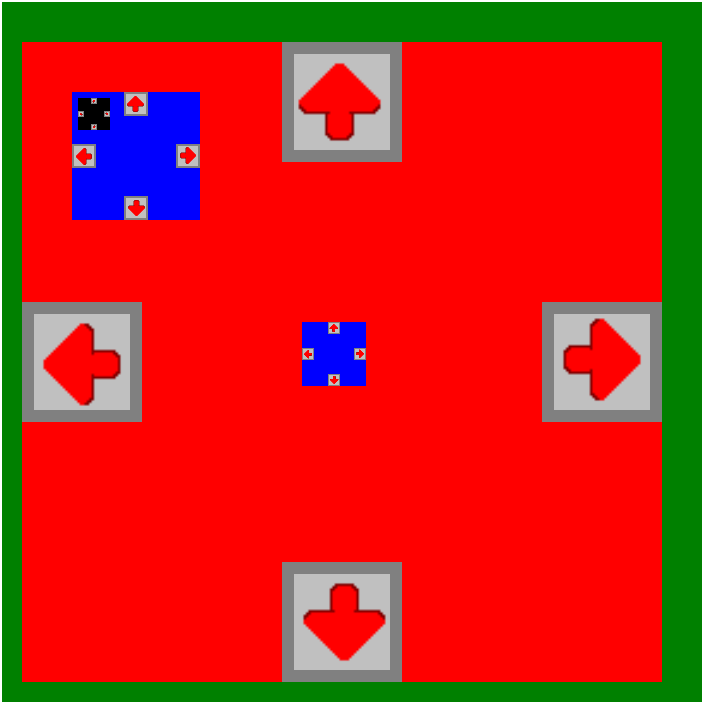
\includegraphics[width=\imglength]{GuiImg}%
	\vspace{-2\ht0}%
\end{wrapfigure}% 

Here \Q@SafeMovable.overlap@ is a static method that simply checks that the bounds of the widgets don't overlap. The call to \Q@this.inside(w1)@ similarly checks that the widget is not outside the bounds of \Q@this@; this instance method call is allowed as \Q@inside(w)@ only uses \Q@this@ to access its \Q!imm! and \Q!rep! fields.

\subheading{Our Experiment}
As shown in the figure below, counting both \Q@SafeMovable@s and \Q@Button@s, our main method creates $21$ widgets: a top level (green) \Q@SafeMovable@ without buttons, containing $4$ (red, blue, and black) \Q@SafeMovable@s with
$4$ (grey) buttons each. When a button is pressed it moves the containing \Q@SafeMovable@ a small amount in the corresponding direction.
This set up is not overly complicated, the maximum nesting level of \Q@Widget@s is $5$.
Our main method automatically presses each of the $16$ buttons once. In L42, using our invariant protocol, this resulted in $77$ calls to \Q@SafeMovable@'s invariant. 

\subheading{Comparison With Visible State Semantics}
As an experiment, we set our implementation to generate invariant checks following the  visible state semantics approaches of D and Eiffel~\cite{Alexandrescu:2010:DPL:1875434,Meyer:1992:EL:129093},
where the invariant of the receiver is instead checked at the start and end of \emph{every} 
public (in D) and qualified\footnote{That is, the receiver is not \Q!this!.} (in Eiffel) method call.

In our \Q!SafeMovable! class, all methods are public, and all calls (outside the invariant) are qualified, thus this difference is irrelevant. Neither protocol performs invariant checks on field accesses or updates,
however due to the `uniform access principle'~\cite{Meyer:1992:EL:129093}%\footnote{%
%L42 also follows the Eiffel uniform access principle: field accesses are the same as method calls.%
%}
, Eiffel allows fields to directly implement methods,
 allowing the \Q!width! and \Q!height! \emph{fields} to directly implement \Q!Widget!'s \Q!width()! and \Q!height()! \emph{methods}. On the other hand in D, one would have to write getter \emph{methods}, which would perform invariant checks.
When we ran our test case following the D approach, the \Q!invariant()! method was called $52,734,053$ times, whereas the Eiffel approach `only' called it $14,816,207$ times;%
\footnote{
This difference is caused by Eiffel treating getters specially, and skipping invariant checks when calling a getter.
Thus, even ignoring getter methods, the visible state semantic would still run 14 millions of invariant checks.
}
in comparison our invariant protocol only performed $77$ calls.
 The number of checks is exponential in the depth of the GUI: the invariant of a \Q@SafeMovable@ will call the \Q@width()@, \Q@height()@, \Q@left()@, and \Q@top()@ methods of its children, which may themselves be \Q@SafeMovable@s, and hence such calls may invoke further invariant checks. Note that \Q!width()! and \Q!height()! are simply getters for fields, whereas the other two are non-trivial \emph{methods}.
Concluding, we have shown that when an invariant check queries other objects with invariants the visible state semantics may cause an exponential explosion in the number of checks.

%though 42 represents field accesses as method calls, for a fair comparison with conventional OO approach, we do not treat field accesses on \Q@SafeMovable@s within the \Q@SafeMovable@ class itself as public method calls
% D and Eiffel have slightly different interpretation of
% visible state semantic when qualified/unqualified method calls or field accesses are performed.
% However, in our GUI example those corner cases are
% not relevant. To be sure, we implemented both of their strategies and obtained the same results.

 % Since we only use \Q@this@ to perform method calls, the invariant is not recursively checked on \Q@this@, if it were we would get an infinite recursion.
% Note that 42 represents field accesses as method calls, this is similar to the Eiffel uniform access principle; but for a fair comparison with D we treat private accesses to them like field accesses.


% It can be surprising to see such extreme difference. We ran our example with less widgets, and our results suggest an exponential growth in the cost of the conventional approach. For example by removing 2 containers (and their 8 buttons) we get....
% We now explain how this exponential explosion happens:
% For the outer-most box to check its invariant, it needs to call methods \Q@left,top,height@ and \Q@with@ to all its contained widgets.
% If one of those widget has \Q@invariant()@, when such public method is called,
% its \Q@invariant()@ is checked (twice). This requires to call \Q@left,top,height@ and \Q@with@ to all its contained widgets, some of those may also have invariants.

% In literature there is attention to prevent method called from an invariant to call public methods on \Q@this@; it would cause the system to go in loop.
% However when calling methods on other objects is allowed, if those objects have invariant, this cause the aforementioned explosion. 

% Our example also shows that the restrictions of TM's and object capabilities's are flexible enough to encode interactive GUI programs, where widgets may circularly reference other widgets.
% In order to perform this case study, we had to first implemented a simple Gui Library in L42. This library uses object capabilities to draw the widgets on screen, as well as fetch and dispatch the events.
% The gui library abstract away all the details of drawing and events; the user code need only to provide concrete classes implementing the \Q@Widget@ interface.

\subheading{Spec\# Comparison}
We also encoded our example in Spec\#\footnote{We compiled Spec\# using the latest available source (from 19/9/2014).}; that relies on pack/unpack; also called inhale/exhale or the Boogie methodology.
In pack/unpack, an object's invariant is checked only by the explicit pack operations.
In order for this to be sound, some form of aliasing and/or mutation control is necessary. Spec\# uses a theorem prover, together with source code annotations.
Spec\# can be used for full static verification, but it conveniently allows invariant checks to be performed at runtime, whilst statically verifying aliasing, purity and other similar standard properties.
This allows us to closely compare our approach with Spec\#.

As the back-end of the L42 GUI library is written in Java, we did not port it to Spec\#, rather we just simulated it, and don't actually display a GUI in Spec\#.
We ran our code through the Spec\# verifier (powered by Boogie~\cite{DBLP:conf/fmco/BarnettCDJL05}), which only gave us $2$ warnings\footnote{We used \Q@assume@ statements, equivalent to Java's \Q@assert@, to dynamically check array bounds. %. and value presence.
This aligns the code with L42, which also performs such checks at runtime.}, because the invariant of \Q@SafeMovable@ was not known to hold at the end of its constructor and \Q@dispatch(e)@ method. Thus, like our system, Spec\# checks the invariant
at those two points at runtime. Thus the code is equivalently verified in both Spec\# and L42; in particular it performed exactly the same number ($77$) of runtime invariant checks.

While the same numbers of checks are performed, we do not have the same guarantee provided by our approach:  Spec\#/Boogie does not soundly handle the non-deterministic impact of I/O, thus 
it does not properly prevent us from writing unsound
invariants that may be non-deterministic.
We also encoded our GUI in Microsoft Code Contracts~\cite{DBLP:conf/sac/FahndrichBL10}, whose unsound heuristic also calls the invariant $77$ times. However Code Contract does not enforce the
encapsulation of \Q@children()@, thus this approach is even less sound than Spec\#.

% Assuming that Spec\#'s verifier is sound, this means that our code is equally verified in Spec\# and L42, providing a reasonable comparison.
% Both Spec\# and L42 did the same thing:
% they statically verify ownership/aliasing annotations,
% they check the admissibility/valididty of a the invariant code and finally 
% they perform sufficient runtime-checking of the invariant.
% We used the Boogie static checker to verify all the aliasing/ownership properties needed to
% ensure that the $77$ run-time invariant checks soundly enforce that the invariant holds when is expected.
% This of course includes preventing the Gui to ever display two overlapping Widget. 

%\end{itemize}
%The result is the same of L42: the invariant is checked $77$ times, and in exactly the same locations of L42.

Note how both our L42 and Spec\# code required us to use the box pattern for our \Q@SafeMovable@, due to the cyclic object graph caused by the \Q@Action@s of \Q@Button@s needing to change their enclosing \Q@SafeMovable@'s position.
We found it quite difficult to encode the GUI in Spec\#, due to its unintuitive and rigid ownership discipline. In particular we needed to use many more annotations, which were larger and had greater variety. The following table shows the annotation burden,
for the \emph{program} that defines and displays the \Q@SafeMovable@s and our GUI; as well as the \emph{library} which defines \Q@Button@s, \Q@Widget@, and event handling. We only count constructs Spec\# adds over C\# as annotations, we also do not count annotations related to array bounds or null checks:
\begin{center}\SS
\begin{tabular}{ c  c  c  c  c}
 & Spec\# & Spec\# & L42 & L42 \\ 
 & \!\!program & library & program & library \\
\hline
 
\!\!\!Total number of annotations 
 	& $40$ & $19$ & $19$ & $18$ \\ \hline
% Totals 	 $59$ $37
\!\!\!Tokens (except \Q@.,;(){}[]@ and whitespace)\!\!\!
%(ecluding \Q@;,@ characters, white-space, or parentheses/brackets.) 
	& $106$ & $34$ & $19$ & $18$  \\  \hline
% $140$  & $37$
Characters (with minimal whitespace) 
	& $619$ & $207$ & $74$ & $60$ \\ \hline
%  $826$ $134$
\end{tabular}
\end{center}
\lstset{morekeywords={requires}}

To encode the GUI example in L42, the only annotations we needed were the 3 reference capabilities: \Q@mut@, \Q@read@, and \Q@capsule@ (\Q!rep! fields in the actual L42 language use the \Q!capsule! keywords to minimise language complexity);
% , for a total of 
% $19$ annotations (one token each, $74$ characters in total).
Our Spec\# code requires purity, immutability, ownership, method pre/post-conditions and method modification annotations. In addition, it requires the use of 4 different ownership functions including explicit ownership assignments. In total we used 18 different kinds of annotations in Spec\#.
The table presents token and character counts to compare against Spec\#'s annotations, which can be quite long and involved, whereas ours are just single keywords.
Consider for example the Spec\# pre-condition on \Q@SafeMovable@'s constructor: \\
\indent\Q@requires Owner.Same(Owner.ElementProxy(children), children);@

% methods and field attributes as well as requires, ensures and modifies clauses, and finally also %explicit ownership assignment statements.
% Spec\# annotation can be involved, as for example \Q@requires Owner.Same(Owner.ElementProxy(children), children);@}

% To estimate the annotation burden we count the number of tokens (excluding \Q@.;,@ and parenthesis).
% This gave us $113$ tokens, that is more then $5$ times the amount needed in L42.
% The total annotation character count is $830$; $10$ times more then L42.


% 40   106+17=113 619+211
%main 11 annotations, 28 + 11 tokens, 118+65 characters
%safemovable 29 annotations, 78+6 tokens, 501+146 characters

%19   34   207+44
% auxLib // 14 annotations, 25 tokens, 155+44 characters
%guiLib// 5 annoations, 9 tokens, 52 characters

% Moreover, in L42 we only use $3$ different kinds of annotations, while in Spec\# we use $15$ kinds of annotations.

\noindent The Spec\# code also required us to deviate from the code style shown in our simplified version: we could not write a usable \Q@children()@ method in \Q@Widget@ that returns a list of children, instead we had to write \Q@children_count()@ and \Q@children(int i)@ methods; we also needed to create a trivial class with a \Q@[Pure]@ constructor (since \Q@Object@'s one is not marked as such). In contrast, the only indirection we had to do in L42 was creating \Q@Box@es by using 
an additional variable in a nested scope.
This is needed to delineate scopes for promotions.
Based on these results, we believe our system is significantly simpler and easier to use
in comparison with Spec\#, that is more verbose but supports a wider range of verification applications.
% On the basis of these results we believe  that our system is easier to use for programmers that are not experts in software verification. %s:case-study
\saveSpace
\section{The Hamster Example in Spec\#}\saveSpace
\label{s:hamster}
\lstset{language={[Sharp]C}, morekeywords={invariant,ensures,requires,expose,exists,capsule}}

In this section we describe exactly why we chose to annotate the example from Section~\ref{s:intro} in the way we did. For brevity, we will assume the default accessibility is \Q@public@, whilst in both Spec\# and C\#, it is actually \Q@private@.

\subheading{The \Q@Point@ Class} 
The typical way of writing a \Q@Point@ class in C\# is as follows:
\begin{lstlisting}
class Point {
	double x, y;
	Point(double x, double y) { this.x = x; this.y = y; }
}
\end{lstlisting}

This works exactly as is in Spec\#, however we have difficulty if we want to define equality of \Q@Point@s (see below).

\subheading{The \Q@Hamster@ Class} 
The \Q@Hamster@ class in C\# would simply be:
\begin{lstlisting}
class Hamster {
	Point pos;
	Hamster(Point pos) { this.pos = pos; }
}
\end{lstlisting}

Though this is legal in Spec\#, it is practically useless. Spec\# has no way of knowing whether \Q@pos@ is \emph{valid} or \emph{consistent}. If \Q@pos@ is not known to be valid, one will be unable to pass it to almost any method, since by default methods implicitly require their receivers and arguments to be valid (compare this with our invariant protocol, which guarantees that any reachable object is valid).
If \Q@pos@ is not known to be consistent, one will be unable to mutate it, by updating one of its fields or by passing it as an argument (or receiver) to a non \Q@Pure@ method.
Though we don't want \Q@pos@ to ever mutate, Spec\# currently has no way of enforcing that an \emph{instance} of a non immutable class is itself immutable\footnote{There is a the describes a simple solution to this problem: assign ownership of the object to a special predefined `freezer' object, which never gives up mutation permission~\cite{DBLP:conf/vstte/LeinoMW08}, however this does not appear to have been implemented; this would provide similar flexibility to the TM system we use, which allows an initially mutable object to be promoted to immutable.}, as such we will simply refrain from mutating it.

To enable Spec\# to reason about \Q@pos@'s validity, we will require that it be a \emph{peer} of the enclosing \Q@Hamster@; we can do this by annotating \Q@pos@ with \Q@[Peer]@. Peers are objects that have the same owner, implying that  whenever one is valid and/or consistent, the other one also is. This means that if we have a \Q@Hamster@, we can use its \Q@pos@, in the same ways as we could use the \Q@Hamster@.

To simplify instantiation of \Q@Hamster@s, their constructors will take unowned \Q@Point@s, Spec\# will then automatically make such \Q@Point@ a peer. This is achieved by taking a \Q@[Captured]@ \Q@Point@ in the constructor (note how similar this is to taking a \Q@capsule@ \Q@Point@). Note that unlike our system, this prevents multiple \Q@Hamster@s from sharing the same \Q@Point@, unless both \Q@Hamster@s have the same owner, if \Q@Point@ were immutable, there would be no such restriction.

With the aforementioned modifications, the \Q@Hamster@ becomes:
\begin{lstlisting}
class Hamster {
  [Peer] Point pos;
  Hamster([Captured] Point pos) { this.pos = pos; }
}
\end{lstlisting}

We don't want \Q@Point@ to be an immutable/value type, however if it were, the original unannotated version would not have any problems.

\subheading{The \Q@Cage@ Class} 
The natural way to write this class in C\#, if it had native support for class invariants like Spec\#, would be:
\begin{lstlisting}
class Cage {
  Hamster h;
  List<Point> path;
  Cage(Hamster h, List<Point> path){this.h=h; this.path=path;}
  invariant this.path.Contains(this.h.pos);
  void Move() { 
    int index = this.path.IndexOf(this.h.pos);
    this.h.pos = this.path[index % this.path.Count]; } 
}
\end{lstlisting}

However for the above \Q@invariant@ to be admissible in Spec\#, \Q@this.path@ and \Q@this.h@ must both be owned by \Q@this@. In addition, the \emph{elements} of \Q@this.path@ need to be owned by \Q@this@, since \Q@this.path.Conatains@ will read them. Note that \Q@this.h.pos@ also needs to be owned by \Q@this@, however since \Q@pos@ is declared as \Q@[Peer]@, if \Q@this@ owns \Q@this.h@, it also owns \Q@this.h.pos@. To fix the invariant, we will declare \Q@h@, \Q@path@, and the elements of \Q@path@ as \emph{reps} (i.e. they are owned by the containing object). Finally, since \Q@Move@ modifies \Q@this.h@, \Q@this.h@ needs to be made consistent, which requires that the owner (\Q@this@) be made invalid; this can be achieved by using an \Q@expose(this)@ statement. \Q@expose(this){@\emph{body}\Q@}@ marks \Q@this@ as invalid, executes \emph{body}, checks that the invariant of \Q@this@ holds, and then marks \Q@this@ valid again.
As we did with the \Q@Hamster@, we will simply take unowned \Q@h@ and \Q@path@ values, however we also need the elements of \Q@path@ to be unowned; since Spec\# has no \Q@[ElementsCaptured]@ annotation, we will require \Q@path@ to be unowned, and its elements (denoted by \Q@Owner.ElementProxy(path)@) to be owned by the same owner as \Q@path@ (which is \Q@null@).
\begin{lstlisting}
class Cage {
  [Rep] public Hamster h;
  [Rep, ElementsRep] List<Point> path;
	
  Cage([Captured] Hamster h, [Captured] List<Point> path)
    requires Owner.Same(Owner.ElementProxy(path), path);
  { this.h = h; this.path = path; }
	
  invariant this.path.Contains(this.h.pos);
  void Move() { 
    int index = this.path.IndexOf(this.h.pos);
    expose(this){this.h.pos=this.path[index%this.path.Count]; }} 
}
\end{lstlisting}

The above constructor now fails to verify, since Boogie is unconvinced that its precondition actually holds when we initialise \Q@this.path@. This is because the constructor for \Q@Object@ (the default base class if none is provided) is not marked as \Q@[Pure]@; since it is (implicitly) called upon entry to \Q@Cage@'s constructor, Boogie has no idea as to what memory could've mutated, and so it doesn't know whether the precondition still holds. The solution is to explicitly call it, but at the end of the constructor: \Q@{this.h = h; this.path = path; base();}@.

The above \Q@Cage@ code however does not work, since \Q@List@ operations, such as \Q@Contains@ and \Q@IndexOf@, will call the virtual \Q@Object.Equals@ method to compute equality of \Q@Point@s. However \Q@Object.Equals@ implements \emph{reference} equality, whereas we want \emph{value} equality.

\subheading{Defining Equality of \Q@Point@s}
The obvious solution in C\# is to just override \Q@Object.Equals@ accordingly, and let dynamic dispatch handle the rest:
\begin{lstlisting}
class Point {
  .. // as before
  override bool Equals(Object? o) {
    Point? that = o as Point;
    return that!=null && this.x == that.x && this.y == that.y;}
}
\end{lstlisting}

However this fails in Spec\# since \Q@Object.Equals@ is annotated with \Q@[Pure]@\\*\Q@[Reads(ReadsAttribute.Reads.Nothing)]@, and of course every overload of it must also satisfy this. The \Q@Reads@ annotations specifies that the method cannot read fields of \emph{any} object, not even the receiver, this makes overloading the method useless.
% Our best guess as to why \Q@Object.Equals@ is annotated like that is that they expect it to be the default reference-equality, annotating it like this could aid static verification as it implies that whether or not two objects are equal cannot change, even if their fields are modified.

We resorted to making our own \Q@Equal@ method. Since it is called in \Q@Cage@'s invariant, Spec\# requires it to be annotated as \Q@[Pure]@, and either annotated with\\* \Q@[Reads(ReadsAttribute.Reads.Nothing)]@ or \Q@[Reads(ReadsAttribute.Reads.Owned)]@\\* (the default, if the method is \Q@[Pure]@). The latter annotation means it can only read fields of objects owned by the \emph{receiver} of the method, so a \Q@[Pure] bool Equal(Point that)@ method can read the fields of \Q@this@, but not the fields of \Q@that@. Of course this would make the method unusable in \Q@Cage@ since the \Q@Point@s we are comparing equality against do not own each other. As such, the simplest solution is to pass the fields of the other point to the method:
\begin{lstlisting}
[Pure] bool Equal(double x, double y) {
  return x == this.x && y == this.y;}
\end{lstlisting}

Sadly however this mean we can no longer use \Q@List@'s \Q@Contains@ and \Q@IndexOf@ methods, rather we have to expand out their code manually; making these changes takes us to the version we presented in Section \ref{s:intro}.

\lstset{language=FortyTwo}

%\subheading{Expressiveness}
%\noindent\textit{Expressiveness:}
%Finally, in our this third case study we 
%shown that even if we do not aim to expressiveness, but to simplicity, soundness and efficiency, we are still able to express a reasonable amount of cases.
%We encoded in L42 all the examples present in papers~\cite{??}.
%We can express all the examples except ....
%Again, we quantify the annotation burden and we discover....

%\subheading{The transform pattern}


%\begin{lstlisting}[escapechar=\%]
%class List {
%  mut List prev;
%  mut List next;
%  Object elem;  
%  read method Bool ok() {
%    return this.next.prev==this && this.prev.next==this &&..;}
%  read method Int size(){
%    if(next==this){return 1;} return next.size()+1;}}
%\end{lstlisting}
%Clearly the \Q@mut@ fields of \Q@List@ cannot be marked as \Q@capsule@.
%However, only \Q@capsule@ and \Q@imm@
%fields can be accessed in \validate.
%Thus, \Q@.innerValidate()@ can not be the \Q@invariant@ method for \Q@List@.
%The solution is to use a `box' over our \Q@List@, and to validate our `box':

%\loseSpace\loseSpace\loseSpace
%\begin{lstlisting}[escapechar=\%]
%class ListBox { 
%  capsule List inner;
%  read method imm Bool invariant() {return this.inner.ok();}
%  read method Int size(){ return this.inner.size();}
%\end{lstlisting}
%\saveSpace
%Encoding this example in Spec\# would be much more verbose (see case study XX) and still require
%a \Q@ListBox@ object,
%while the visible state semantic of Eiffel or D would cause an large amount of \Q@invariant@ checks
%if the list had any recursive method; consider for example the \Q@size@ method:
%if there was an invariant with visible state semantic on \Q@List@, calling \Q@List.size()@ would require 
%calling \Q@List.invariant()@ before and after the method execution. If the list has more then one element, the recursive \Q@size@ call would also call the invariant twice.
%We would also want to create forwarding methods in \Q@ListBox@ for all public methods defined in \Q@List@. This approach allows the validation of many interesting and practically useful data-structures.
%However the limitations of capsule mutator methods mean that any \Q@mut@ methods in \Q@ListBox@ taking \Q@read@ or \Q@mut@ parameters, or returning \Q@mut@, cannot be trivially forwarded.
%% since they necessitate mutating a \Q@capsule@, instead complicated and involved forwarding would be needed, if it is even possible.
%Our example is about a list of immutable objects.
%To instead validate a list of \Q@mut@ objects we would need to use our box pattern not just around the list,
%but around a section of data encapsulating both the list and all the contained elements.
%This is because our simple \Q@capsule@ modifier requires the whole ROG to be encapsulated.
%Conceptually, it would be better for the list (of mutable objects) to be validated by its
%head, since the behaviour of the contained objects is transparent to the validation criteria. 
%Our limitation relates to full encapsulation and contrasts with flexible encapsulation as in 
%ownership~\cite{ClarkeEtAl98}. However, neither traditional flexible encapsulation/ownership, nor our language are capable of verifying that \Q@List.elem@ is not (indirectly) referenced within \Q@ListBox.validate()@.


%\subheading{Family, a worst case scenario for L42}
%\noindent\textit{Family, a worst case scenario for L42}
%For our second case study, we wished to make an example where the performance of L42 and the conventional approach was similar. We forged an example when a \Q@Family@ has a list of parents and a list of children;
%all the children need to be younger then their parents and every \Q@Person@ need to have a non empty name and a positive age.  
%We model the pass of time with a \Q@processDay@ method, and we simulate $3$ years of life (that is, $3\times365$ days) of a family of $4$.
%The age of a \Q@Person@ grow when its birthday is processed.
%Notably, \Q@processDay@ is a \Q@mut@ method that can potentially mutate any person in the system, thus
%L42 have to run a lot of invariant checks. The object graph here is very shallow: the \Q@Family@ holds the \Q@Person@s and that is it.
%However, even in this case we get about $9$ times less invariant calls: $19403$ with visible state semantic  and $2210$ in L42.
%Also the \Q@Family@ example uses the box pattern.

%\subheading{Family}
%We wished to make an example where the performance of L42 and the conventional approach 
%was similar. We forged an example when a Family has a list of parents and a list of children;
%all the childrens need to be younger then their parents and every Person need to have a non empty name and a positive age.  
%We model the pass of time with a \Q@processDay@ method, and we simulate 3 years of life (that is, 3*365 days) of a family of 4.
%The age of a Person grow when its birthday is processed.
%Notably, \Q@processDay@ is a mut method that can potentially mutate any person in the system, thus
%L42 have to run a lot of invariant checks. The object graph here is very shallow: the Family holds the Persons and that is it.
%However, even in this case we get about 10 times less invariant calls: Num in the conventional approach and Num in L42.

%\subheading{Spec\# 2papers}
%Our goal in this third case study was to show that even if we do not aim to expressiveness, but to simplicity, soudness and efficiency, we are still able to express a reasonable amount of cases.
%We can express all the examples except ....
%Again, we quantify the annotation burden and we discover....

%\section{Stack overflow and Out of memory}
%For our system to be sound,
%Stack overflow and Out of memory errors need to be modeled specially.
%If they are just (unchecked) exceptions then they could be catched to 
%generate non deterministic behaviour inside invariant code.

%However, it is possible to use capaility objects to capture them as special system events/signals.
%In this way we can maintain the soundness of our system even in this corner case.
%Of course, another option would be to make them into unrecoverable fatal errors.

\lstset{morekeywords={expose}}

\section{More Case Studies}
\label{s:MoreCaseStudies}
\subheading{Graph}

Here we present an example where a general \Q@Graph@
of \Q@Node@s can be defined as a library,
and the user of the library can define personalized kinds of nodes,
with their personalized (sub-)invariant \Q@subInvariant@.
The library will ensure that no matter how it is used, all the 
user defined sub invariants of the inner nodes are preserved.
The \Q@Node@s, even if user defined, are guaranteed to be encapsulated by the \Q@Graph@.
The \Q@Graph@ can be arbitrarily modified by user defined transformations using the Transform Pattern.
\begin{lstlisting}
interface Transform<T>{method read T apply(mut Nodes nodes);}

interface Node{
  read method Bool subInvariant(read Nodes nodes)
  mut method mut Nodes directConnections()
  }
class Nodes{//just an ordered set of nodes 
  mut method Void add(mut Node n){..}
  read method Int indexOf(read Node n){..}
  mut method Void remove(read Node n){..}
  mut method mut Node get(Int index){..}
  }
class Graph{ 
  capsule Nodes nodes; //box pattern
  Graph(capsule Nodes nodes){..}
  read method read Nodes getNodes(){return this.nodes;}
  <T> mut method read T transform(Transform<T> t){
    mut Nodes ns=this.nodes;//capsule mutator single 'this' use
    return t.apply(ns);
    }
  read method Bool invariant(){
    for(read Node n: this.nodes){
      if(!n.subInvariant(this.nodes)){return false;}
      }
    return true;
    } }
\end{lstlisting}
Note how there is basically no logic in the above code.
All the logic can be freely defined by the user code, as shown below:

\begin{lstlisting}
class MyNode{
  mut Nodes directConnections;
  mut method mut Nodes directConnections(){
    return this.directConnections;}
  MyNode(mut Nodes directConnections){..}
  read method Bool subInvariant(read Nodes nodes){
    /*any condition on either this, nodes or the connections*/}  
  capsule method read MyNode addToGraph(mut Graph g){..}
  read method Void connectWith(read Node other,mut Graph g){..}
  }

mut Graph g=new Graph(new Nodes());
read MyNode n1=new MyNode(new Nodes())).addToGraph(g);
read MyNode n2=new MyNode(new Nodes())).addToGraph(g);
//lets connect our two nodes
n1.connectWith(n2,g);
\end{lstlisting}
Here we define a \Q@MyNode@ class, where the subinvariant can express any property over \Q@this@, or the direct connections of \Q@this@, or any other node in graph and their connections.

We can define methods in \Q@MyNode@ to add our nodes
to graphs and to connect with other nodes.
Note that the method \Q@addToGraph@ is \Q@capsule@; this ensures that the node is not in any other graph.
On the other side, the method \Q@connectWith@ takes a \Q@read this@, even if it clearly intend to modify the ROG of \Q@this@.
It works by recovering a \Q@mut@ reference to \Q@this@ from the \Q@mut Graph@.

We now examine the implementation of those two methods:
\begin{lstlisting}
  read method Void connectWith(read Node other,mut Graph g){
    Int i1=g.getNodes().indexOf(this);
    Int i2=g.getNodes().indexOf(other);
    if(i1==-1 || i2==-1){throw /*error nodes not in g*/;}
    g.transform(ns->{
      mut Node n1=ns.get(i1);
      mut Node n2=ns.get(i2);
      n1.directConnections().add(n2);
      });
    }
  capsule method read MyNode addToGraph(mut Graph g){
    return g.transform(ns->{
      mut MyNode n1=this;//single usage of capsule 'this'
      ns.add(n1);
      return n1;
      });
    }
\end{lstlisting}
As you can see, both methods relies on the Transform Pattern.

Those transformation operations are very general since they
can take in input the \Q@mut Nodes@ content of the graph and 
any \Q@capsule@ or \Q@imm@ data from outside.
Note how in \Q@connectWith@ we can not see the \Q@read this@ or the \Q@read other@
inside the lambda, but we need to get their (immutable) indexes 
and recover the concrete objects from the \Q@mut Nodes ns@ object.
In this way, we also obtain more useful \Q@mut@ references to those nodes.
On the other side, note how in \Q@addToGraph@ we can see the reference to \Q@capsule this@ inside the lambda.

Concluding, our approach imposes a very defensive programming style
that is not currently commonly used in programming practice.
But with a little bit of experience using our system, any data structure can be defined.
Any invariant relying only on immutable and encapsulated state can be enforced; and any transformation based on immutable and capsule input can be defined.

\subheading{Family}
The following test case was designed to produce a worst case in the number of invariant checks. We have a \Q!Family! that (indirectly) contains a list of \Q!parents! and \Q!children!. The \Q!parents! and \Q!children! are of type \Q!Person!. Both \Q!Family! and \Q!Person! have an invariant, the invariant of \Q!Family! depends on its contained \Q!Person!s.

% TODO: Talk to mark about code style

% TODO: Swap parent/child updates in aritifact
\begin{lstlisting}
class Person { 
  final String name;
  Int daysLived;
  final Int birthday;
  Person(String name, Int daysLived, Int birthday) { .. }
  mut method Void processDay(Int dayOfYear) {
  	this.daysLived += 1;
    if (this.birthday == dayOfYear) {
    	Console.print("Happy birthday " + this.name + "!"); }}
  read method Bool invariant() {
    return !this.name.equals("") && this.daysLived >= 0 &&
      this.birthday >= 0 && this.birthday < 365; }
}
class Family { 
  static class Box { 
    mut List<Person> parents;
    mut List<Person> children;
    Box(mut List<Person> parents, mut List<Person> children){..}
    mut method Void processDay(Int dayOfYear) {
      for(Person c : this.children) { c.processDay(dayOfYear); }
      for(Person p : this.parents) { p.processDay(dayOfYear); }}
  }
  capsule Box box;
  Family(capsule List<Person> ps,capsule List<Person> cs) {
    this.box = new Box(ps, cs); }
  mut method Void processDay(Int dayOfYear) { 
    this.box.processDay(dayOfYear); }
  mut method Void addChild(capsule Person child) { 
    this.box.children.add(child); }
  read method Bool invariant() {
    for (Person p : this.box.parents) {
      for (Person c : this.box.children) {
        if (p.daysLived <= c.daysLived) { 
          return false; }}}
    return true; }
}
\end{lstlisting}
Note how we created a \Q!Box! class to hold the \Q!parents! and \Q!children!.
Thanks to this pattern, the invariant only needs to hold at the end of \Q!Family.processDay!, after all the \Q!parents! and \Q!children! have been updated. Thus \Q!Family.processDay! is atomic: it updates all its contained \Q!Person!s together.
%This capture the intention of consistently calling \Q@Person.processDay@ once for all the persons as an atomic operation.
%This capture the intention of atomically and consistently calling \Q@Person.processDay@ once for all the persons.
Had we instead made the \Q!parents! and \Q!children! \Q!capsule! fields of \Q!Family!, the invariant would be required to also hold between modifying the two lists. This could cause problems if, for example, a child was updated before their parent.

%\loseSpace
We have a simple test case that calls \Q!processDay! on a \Q!Family! $1{,}095$ ($3\times365$) times.
%$3\times365$ times ($1{,}095$ days):
\begin{lstlisting}
// 2 parents (one 32, the other 34), and no children
var fam = new Family(List.of(new Person("Bob", 11720, 40),
    new Person("Alice", 12497, 87)), List.of());
    
for (Int day = 0; day < 365; day++) { // Run for 1 year
  fam.processDay(day);
}
for (Int day = 0; day < 365; day++) { // The next year
  fam.processDay(day);
  if (day == 45) {
    fam.addChild(new Person("Tim", 0, day)); }}

for (Int day = 0; day < 365; day++) { // The 3rd year
  fam.processDay(day);
  if (day == 340) {
    fam.addChild(new Person("Diana", 0, day)); }}
\end{lstlisting}
% The counts (including the invariant keyword, and read on the invariant method)
% Spec# 14 family, 2 main   = 16
% L42 	12 family, 1 person = 14
% Fake 42 = 14 (+2 for box ctor, -1 for family ctor)

The idea is that everything we do with the \Q!Family! is a mutation; the \Q!fam.processDay! calls also mutate the contained \Q!Person!s.

This is a worst case scenario for our approach compared to visible state semantics since it reduces our advantages:
our approach avoids invariant checks when objects are not mutated
but in this example most operations are mutations; 
similarly, our approach prevents the exponential explosion of nested invariant checks\footnote{As happened in our GUI case study, see Section \ref{s:case-study}.} when deep object graphs are involved, but in this example the object graph of \Q!fam! is very shallow.
%\loseSpace

We ran this test case using several different languages: L42 (using our protocol) performs $4{,}000$ checks, D and Eiffel perform $7{,}995$, and finally, Spec\# performs only $1{,}104$.

Our protocol performs a single invariant check at the end of each constructor,  \Q!processDay! and \Q!addChild! call (for both \Q!Person! and \Q!Family!). 

The visible state semantics of both D and Eiffel perform additional invariant checks at the beginning of each call to \Q!processDay! and \Q!addChild!.

The results for Spec\# are very interesting, since it performs less checks than L42.
This is the case since \Q!processDay! in \Q!Person! just does a simple field update, which in Spec\# do not invoke runtime invariant checks. Instead, Spec\# tries to statically verify that the update cannot break the invariant; if it is unable to verify this, it requires that the update be wrapped in an \Q!expose! block, which will perform a runtime invariant check. 

Spec\# relies on the absence of arithmetic overflow, and performs runtime checks to ensure this%
\footnote{%
Runtime checks are enabled by a compilation option; when they fail, unchecked exceptions are thrown.%
}, as such the verifier concludes that the field increment in \Q!processDay! cannot break the invariant.
Spec\# is able to avoid some invariant checks in this case 
by relying on all arithmetic operations performing runtime overflow checks;
whereas integer arithmetic in L42 has the common wrap around semantics.
%L42's integers have common wrap-around semantic.


%\footnote{%
%Such semantic can be enforced by
%a compilation option, disabled on default for performance reasons.
%Overflow is detected at runtime, by throwing an unchecked exceptions; just as for invariant failures.%
%}

% Concluding Spec\# is able to replaces some runtime invariant checks with more efficient runtime overflow checks.


%This is the case since \Q!processDay! in \Q!Person! just does a simple field increment, thus the Spec\# verifier is able to statically verify that this wont break the invariant, and so it does not require a corresponding \Q!expose! block, and hence does not perform a runtime invariant check.
%The Spec\# verifier is able to do this as it works on a language semantic where arithmetic overflow does not occur. Such semantic can be enforced by
%a compilation option (disable on default for performance reasons).
%%%%however one can turn on runtime checking for overflow.
%%%and check overflow errors at run time
%With this option turned on, eliding the invariant check is sound since overflow will have the same result as a runtime invariant check failure, namely it will throw an unchecked exception.


%This static reasoning is performed under the assumption that arithmetic overflow will not occur, thus Spec\# is considering a different semantic for \Q@Int@ then L42. Spec\# can inject run-time checks to enforce such arithmetic semantic.


The annotations we had to add in the Spec\# version\footnote{The Spec\# code is in the artifact.} were similar to our previous examples, however since the fields of \Q!Person! all have immutable classes/types, we only needed to add the invariant itself. The \Q!Family! class was similar to our \Q!Cage! example (see Section \ref{s:intro}), however in order to implement the \Q!addChild! method we were forced to do a shallow clone of the new child (this also caused a couple of extra runtime invariant checks). Unlike L42 however, we did not need to create a box to hold the \Q!parents! and \Q!children! fields, instead we wrapped the body of the \Q!Family.processDay! method in an \Q!expose (this)! block. In total we needed 16 annotations, worth a total of 45 tokens, this is worse than the code following our approach that we showed above, which has 14 annotations and 14 tokens.


\subheading{Spec\# Papers}
Their are many published papers about the pack/unpack methodology used by Spec\#. To compare against their expressiveness we will consider the three mains ones that introduced their methodology and extensions:
\SSI\begin{itemize}
	\item \emph{Verification of Object-Oriented Programs with Invariants:}~\cite{DBLP:journals/jot/BarnettDFLS04} this paper introduces their methodology. In their examples section (pages 41--47), they show how their methodology would work in a class heirarchy with \Q!Reader! and \Q!ArrayReader! classes. The former represents something that reads characters, whereas the latter is a concrete implementation that reads from an owned array. They extend this further with a \Q!Lexer! that owns a \Q!Reader!, which it uses to read characters and parse them into tokens. They also show an example of a \Q!FileList! class that owns an array of filenames, and a \Q!DirFileList! class that extends it with a stronger invariant. All of these examples can be represented in L42\footnote{Our encodings are in the artifact.}. The most interesting considerations are as follow:
	\begin{itemize}
		\item Their \Q!ArrayReader! class has a \Q!relinquishReader! method that `unpacks' the \Q!ArrayReader! and returns its owned array.
%This allows other code to mutate the array freely,
%Then other code can mutate such relinquished array freely.
The returned array can then be freely mutated and passed around by other code.
%at the cost of being unable to use the \Q!ArrayReader! until it is packed again
However, afterwards the \Q!ArrayReader! will be `invalid', and so one can only call methods on it that do not require its invariant to hold. However, it may later be `packed' again (after its invariant is checked).
%Due to our guarantee that usable objects must have their invariant hold, we are unable to do this.
In contrast, our approach requires the invariant of all usable objects to hold.
%In our approach we do not have any visible unusable objects. 
We can still relinquish the array, but at the cost of making the \Q!ArrayReader! forever unreachable. This can be done by
% However, we can
 declaring \Q!relinquishReader! as a \Q!capsule method!, this works since our type modifier system guarantees that the receiver of such a method is not aliased, and hence cannot be used again. Note that Spec\# itself cannot represent the \Q!relinquishReader! method at all, since it does not provide explicit pack and unpack operations, rather its \Q!expose! statement performs both an unpack and a pack, thus we cannot unpack an \Q!ArrayReader! without repacking it in the same method.
%(unless we were to throw an unchecked-exception, however this is unsound~\cite{Leino2004ExceptionSF}).
		\item Their \Q!DirFileList! example inherits from a \Q!FileList! which has an invariant, and a final method, this is something their approach was specifically designed to handle. As L42 does not have traditional subclassing, we are unable to express this concept fully, but L42 does have code reuse via trait composition, in which case \Q!DirFileList! can essentially copy and paste the methods from \Q!FileList!, and they will automatically enforce the invariant of \Q!DirFileList!. %The disadvantage however is that if \Q!FileList! is a trait, it cannot also be a type, and so we cannot have a non-final type/class with a concrete invariant, however one can always have a final class with an invariant that wraps over a non final one. This is not an inherent limitation with our invariant protocol, but rather one of the L42 language itself.
	\end{itemize}

	\item \emph{Object Invariants in Dynamic Contexts:}~\cite{leino2004object} this paper shows how one can specify an invariant for a doubly linked list of \Q!int!s (here \Q!int! is an immutable value type). Unlike our protocol however, it allows the invariant of \Q!Node! to refer to sibling \Q!Node!s which are not owned/encapsulated by itself, but rather the enclosing \Q!List!. Our protocol can verify such a linked list\footnote{%
Our protocol allows for encoding this example, but
to express the invariant we would need to 
use reference equality, which the L42 language does not support.
%We were unable to implement this in L42, as the invariant uses reference equality, which the language does not implement.
} (since its elements are immutable), however we have to specify the invariant inside the \Q!List! class. We do not see this as a problem, as the \Q!Node! type is only supposed to be used as part of a \Q!List!, thus this restriction does not impact users of \Q!List!.
	
	\item \emph{Friends Need a Bit More: Maintaining Invariants Over Shared State:}~\cite{DBLP:conf/mpc/BarnettN04} this paper shows how one can verify invariants over interacting objects, where neither owns/contains the other. They have multiple examples which utilise the `subject/observer' pattern, where a `subject' has some state that an `observer' wants to keep track of. In their \Q!Subject!/\Q!View! example, \Q!View!s are created with references to \Q!Subject!s, and copies of their state. When a \Q!Subject!'s state is modified, it calls a method on its attached \Q!View!s, notifying them of this update. The invariant is that a \Q!View!'s copy of its \Q!Subject!'s state is up to date. Their \Q!Master!/\Q!Clock! example is similar, a \Q!Clock! contains a reference to a \Q!Master!, and saves a copy of the \Q!Master!'s time. The \Q!Master! has a \Q!Tick! method that increases its time, but unlike the \Q!Subject!/\Q!View! example, the \Q!Clock! is not notified. The invariant is that the \Q!Clock!'s time is never ahead of its \Q!Master!'s. Our protocol is unable to verify these interactions, because the
interacting objects are not immutable or encapsulated by each other.
\end{itemize}
\section{Patterns}
\label{s:patterns}
\lstset{morekeywords={invalid}}

In this section we show programming patterns that allow various kinds of invariants.
Our goal is not to verify existing code or patterns,
but to create a simple system that allows soundly verifying the correctness of data structures.
In particular, as we show, in order to use our approach to ensure invariants, one has to program in an uncommon and very defensive style.
%The trade off is that programmers may need to spend more effort in understanding their invariants and encoding them, but less effort in understanding the underlying programming language.

\subheading{The SubInvariant Pattern}
We showed how the box pattern can be used to write invariants over cyclic mutable object graphs, the latter also shows how a complex mutation can be done in an `atomic' way, with a single invariant check. However the box pattern is much more powerful.

 Suppose we want to pass a temporarily `broken' object to other code as well as perform multiple field updates with a single invariant check. 
Instead of adding new features to the language, like an \Q!invalid! modifier (denoting an object whose invariant does not need to hold), and an \Q!expose! statement like Spec\#, we can use a `box' class and a rep mutator to the same effect:
\begin{lstlisting}
interface Person{ mut method Bool accept(read Account a,read Transaction t); }
interface Transaction{ mut method List<Transfer> compute(); }
//Here List<T> represents a list of immutable Ts.
class Transfer{ Int money;
  method Void execute(mut AccountBox that){// Gain some money, or lose some money
    if(this.money>0){ that.income+=money; }
    else{ that.expenses -= money; }
  }
}
class AccountBox{
  UInt income=0; UInt expenses=0;
  read method Bool subInvariant(){ return this.income >= this.expenses; }
  //An `AccountBox' is like a `potentially invalid Account':
  //we may observe income >= expenses
}
class Account{
  rep AccountBox box; mut Person holder;
  read method Bool invariant(){ return this.box.subInvariant(); }
  // `h' could be aliased elsewhere in the program
  Account(mut Person h){ this.holder=h; this.box=new AccountBox(); }
  mut method Void transfer(mut Transaction ts){
    if(this.holder.accept(this, ts)){ this.transferInner(ts.compute()); }
  }
  // rep mutator, like an `expose(this)' statement
  private mut method Void transferInner(List<Transfer> ts){
     mut AccountBox b = this.box;
     for (Transfer t : ts) { t.execute(b); }
  }// check the invariant here
}
\end{lstlisting}
The idea here is that \Q!transfer(ts)! will first check to see if the account holder wishes to accept the transaction, it will then compute the full transaction (which could cache the result and/or do some I/O), and then execute each transfer in the transaction. We specifically want to allow an individual \Q!Transfer! to raise the \Q!expenses! field by more than the \Q!income!, however we don't want an entire \Q!Transaction! to do this. 
Our rep mutator (\Q!transferInner!) allows this by behaving like a Spec\# \Q!expose! block: during its body (the \Q!for! loop) we don't know or care if \Q!this.invariant()! is \Q!true!, but at the end it will be checked. For this to make sense, we make \Q!Transfer.execute! take an \Q!AccountBox! instead of an \Q!Account!: it cannot assume that the invariant of \Q!Account! holds, and it is allowed to modify the fields of \Q!that! without needing to check it. Though rep mutators can be used to perform batch operations like the above, they can only take immutable and capsule objects. This means that they can perform no non-deterministic I/O (due to our object capabilities system), and other externally accessible objects (such as a \Q!mut Transaction!) cannot be mutated during such a batch operation.

As you can see, adding support for features like \Q!invalid! and \Q!expose! is unnecessary, and would likely require making the type system significantly more complicated as well as burdening the language with more core syntactic forms.

In particular, the above code demonstrates that our system can:
\begin{itemize}
\item Have useful objects that are not entirely encapsulated: the \Q!Person holder! is a \Q!mut! field; this is fine since it is not mentioned in the \Q!invariant()! method.
\item Wrap normal methods over rep mutators: \Q!transfer! is not a rep mutator, so it can use \Q!this! multiple times and take a \Q!mut! parameter.
\item Perform multiple state updates with only a single invariant check: the loop in \Q!transferInner(ts)! can perform multiple field updates of \Q!income! and \Q!expenses!, however the \Q!invariant()! will only be checked at the end of the loop.
\item Temporarily break an invariant: it is fine if during the \Q!for! loop, \Q!expenses > income!, provided that this is fixed before the end of the loop.
\item Pass the state of an `invalid' object around, in a safe manner: an \Q!AccountBox! contains the state of \Q!Account!, but not the invariant method.
Note how programmers can use conventional private types to control how such `invalid' versions of objects are exposed in the public API, for example by 
declaring \Q@AccountBox@ as a private nested class.
In contrast, if \Q@invalid@ was a type system feature, then any user defined type would intrinsically expose the existence of both variants in the public API.
\end{itemize}

Under our strict invariant protocol, the invariant holds for all reachable objects.
The sub invariant pattern allows to control when an object is required to be valid.
Instead, other protocols strive to allow the invariant to be observed broken in controlled conditions defined by the protocol itself.

The sub invariant pattern offers interesting guarantees:
any object `\Q@a@' with a \Q@subInvariant()@ method that is checked by the \Q@invariant()@ method of an object `\Q@b@'
will respect its \Q@subInvariant()@ in all contexts where `\Q@b@' is involved in execution.
This is because whenever `\Q@b@' is involved in execution, its invariant holds.
Moreover, \Q@a@'s \Q@subInvariant()@ can be observed as \Q@false@ only if a rep mutator of `\Q@b@' is currently active (that is, being executed),
or \Q@b@ is now garbage collectable.
Thus, even when there is no reachable reference to \Q@b@ in the current stack frame,
if no rep mutator on \Q@b@ is active, \Q@a@'s \Q@subInvariant()@ will hold.

In the former example, this means that
if you can refer to an \Q!Account!, you can be sure that its \Q!income >= expenses!;
if you have an \Q!AccountBox! then you can be sure that either \Q!income >= expenses! or 
a rep mutator of the corresponding \Q@Account@ object is currently active.
This closely resembles some visible state semantic protocols, aiming to ensure that  
either an object's invariant holds, or one of its methods is currently active.


Another interesting and natural application of the sub invariant pattern would be to support a version of the GUI such that, when a \Q@Widget@'s position is updated, the \Q@Widget@ can in turn update the coordinates of its parent \Q@Widget@s, in order to re-establish their \Q@subInvariants@.
This would also make the GUI follow the versions of the composite pattern were objects have references to their `parent' nodes.
The main idea is to define an interface \Q@HasSubInvariant@ that denotes \Q@Widgets@ with a \Q@subInvariant()@ method. Then, \Q@WidgetWithInvariant@ is a decorator over a \Q@Widget@; the invariant method of a \Q@WidgetWithInvariant@ checks the \Q@subInvariant()@ of each contained widget.

%How to apply "Widget; the invariant method of a Widget This Invariant-->Widget and its invariant method" here?

We define \Q@SafeMovable@ as a \Q@Widget@ and \Q@HasSubInvariant@. Since \Q@subInvariant()@ methods don't have the restrictions of invariant methods, it allows \Q@SafeMovable@ to be significantly simpler than the version shown before in \autoref{s:case-study}.
\begin{lstlisting}
interface HasSubInvariant{ read method Bool subInvariant(); }

class SafeMovable implements Widget,HasSubInvariant {
  Int width = 300; Int height = 300;
  Int left; Int top;  // Here we do not use a box, thus all the state
  mut Widgets c;      // is in SafeMovable.
  mut Widget parent;//We add a parent field

  @Override read method Int left(){ return this.left; }
  @Override read method Int top(){ return this.top; }
  @Override read method Int width(){ return this.width; }
  @Override read method Int height(){ return this.height; }
  @Override read method read Widgets children(){ return this.c; }
  @Override mut method Void dispatch(Event e){
    for(mut Widget w :this.c){ w.dispatch(e); }
  }
  @Override read method Bool subInvariant(){ /*same of original GUI*/ }

  SafeMovable(mut Widget parent,mut Widgets c){
    this.c=c;          //SafeMovable no longer has an invariant,
    this.left=5;       //so we impose no restrictions on its constructor
    this.top=5;
    this.parent=parent;
    c.add(new Button(0,0,10,10,new MoveAction(this));
  }
}

class MoveAction implements Action{
  mut SafeMovable o;
  MoveAction(mut SafeMovable o){ this.o = o; }
  mut method Void process(Event e){
    this.o.left+=1;
    Widget p = this.o.parent;
    ... // mutate p to re-establish its subInvariant
  }
}
class WidgetWithInvariant implements Widget{
  rep Widget w;
  @Override read method Int left(){ return this.w.left; }
  @Override read method Int top(){ return this.w.top; }
  @Override read method Int width(){ return this.w.width; }
  @Override read method Int height(){ return this.w.height; }
  @Override read method read Widgets children(){ return this.w.c; }
  @Override mut method Void dispatch(Event e){ w.dispatch(e); }
  @Override read method Bool invariant(){ return wInvariant(w); }
  static method Bool wInvariant(read Widget w){
    for(read Widget wi:w.children()){ if(!wInvariant(wi)){ return false; } }
    //Check that the subInvariant of all of w's descendants holds
    if(!(w instanceof HasSubInvariant)){ return true; }
    HasSubInvariant si = (HasSubInvariant)w;
    return si.subInvariant();
  }
  WidgetWithInvariant(capsule Widget w){ this.w = w; }
}
... // main expression
//#$\$$ is a capability operation making a Gui object
mut Widget top=new WidgetWithInvariant(new SafeMovable(...))
Gui.#$\$$().display(top);
\end{lstlisting}
In this way, the method \Q@WidgetWithInvariant.dispatch()@ is the only rep mutator, hence the only invariant checks will be at the end of \Q@WidgetWithInvariant@'s constructor and dispatch methods.

Importantly, this allows the graph of widgets to be cyclic and for each to freely mutate each
other, even if such mutations (temporarily) violate their \Q@subInvariant@'s.
In this way a widget can access its parent (whose \Q@subInvariant()@ may not hold) in order to re-establish it.
Note that this trade off is logically unavoidable:
in order to manipulate a parent in order to fix it, the parent must be reachable, but
by mutating a \Q@Widget@'s position, its parent may become invalid.
Thus if \Q@Widget@s were to encode their validity in their \Q@invariant()@ methods they could not have access to their parents.
Instead, by encoding their validity in a \Q@subInvariant()@ method,
they can access invalid widgets, but this comes at a cost: the programmer must
reason as to when \Q@Widgets@ are valid, as we described above.


\subheading{The Transform Pattern}
Recall the GUI case study from \autoref{s:case-study}, where we had a \Q!Widget! interface and a \Q!SafeMovable! (with an invariant) that implements \Q!Widget!.
% A rep mutator method is essentially a mutation of a field, which is guaranteed to not see the \Q@this@ object.
% Thus, if \Q@this@ is made invalid during  the method's execution, we could not observe it until after the method completes.
Suppose we want to allow \Q@Widget@s to be scaled, we could add \Q@mut@ setters for \Q@width()@, \Q@height()@, \Q@left()@, and \Q@top()@ in the \Q@Widget@ interface. However, if we also wish to scale its children we have a problem, since \Q@Widget.children()@ returns a \Q@read Widgets@, which does not allow mutation. We could of course add a \Q@mut@ method \Q@zoom(w)@ to the \Q@Widget@ interface, however this does not scale if more operations are desired. If instead \Q@Widget.children@ returned a \Q@mut Widgets@, it would be difficult for \Q@Widget@ implementations, such as \Q@SafeMovable@, 
to mention their \Q!children()! in their \Q!invariant()!.
% In the above \Q@SafeMovable@ we only had one rep mutator: \Q@dispatch@. However suppose a \Q@Widget@ wants to directly mutate it's descendents, however it can't do that since \Q@Widget.children@ returns a \Q@read Widgets@, if it returned a \Q@mut Widgets@ then \Q@SafeMovable@ could not be implement, as it's children are contained inside a capsule-field. 
% At first glance, it may seem that rep mutators allow only very limited kinds %of mutation.
% This is however not the case. 
% Consider the following
% simple pattern to allow flexible use of encapsulated content: define a
A simple and practical solution would be to define a \Q@transform(t)@ method in \Q@Widget@, and a \Q@Transformer@ interface 
like so:
%\footnote{A more general transformer could return a generic \Q@read R@.}
\begin{lstlisting}[escapechar=\%]
interface Transformer<T> { capsule method Void apply(mut T elem); }

interface Widget { ...
  mut method Void top(Int that); // setter for immutable data
  // transformer for possibly encapsulated data
  mut method read Void transform(capsule Transformer<Widgets> t);
}
class SafeMovable implements Widget { ...
  // A well typed rep mutator
  mut method Void transform(capsule Transformer<Widgets> t) {t.apply(this.box.c);}}
\end{lstlisting}
% Note that the code above does not access a \Q!capsule! field but merely calls a method that does; thus  it is \emph{not} a rep mutator method, so it is not constrained by the restrictions on them. Code like the above would also allow one to mutate multiple \Q!capsule! fields in one method.
%Our pattern cooperates with the language’s restrictions to ensure each mutation is completed as a separate operation, that is perceived by the rest of the system %as if it was atomic.%
%,  i.e. they can't see or update the other \Q!capsule! fields.
The \Q@transform@ method offers an expressive power similar to \Q@mut@ getters, but prevents \Q@Widgets@ from leaking out.\footnote{\IO[32]{Note how this kind of pattern solves a similar problem in ownership systems where an object cannot be modified except under the control of the owner. In our example example, this would correspond to the \Q!SafeMovable! being the `owner' of it's `box.c' field.}}  With a \Q@Transformer@, a \Q@zoom(w)@ function could be simply written as:
\begin{lstlisting}
static method Void zoom(mut Widget w) {
  w.transform(ws -> { for (wi : ws) { zoom(wi); } });
  w.width(w.width() / 2); ...; w.top(w.top() / 2); 
}
\end{lstlisting}

In the context of reference capabilities, \Q@capsule@ lambdas/closures will only be allowed to capture \Q@imm@ and \Q@capsule@ local variables.
Note that the \Q@Transformer@ parameter to \Q@transform@ is \Q@capsule@ and the method \Q@Trasformer.apply@ takes a \Q@capsule@ receiver. In particular, this means that \Q@transform@ will be able to call the lambda at most once,
and that those lambdas cannot be saved and passed to multiple calls to \Q@transform@.
However, we could instead make \Q@transform@ take an \Q@imm@ \Q@Transformer@, and make \Q@Transformer.apply@ be an \Q@imm@ method. This would allow those lambdas to be freely copied and called multiple times, however they would only be able to capture \Q@imm@ local variables.
%not be able to capture pre-existing mutable objects.

Here, we assume lambdas, as in Java, are sugar for normal objects that implement an interface with a single abstract method.
As an example, we could use the following sound rules to determine what lambdas are allowed:
\Q!imm! lambda objects implementing an interface with an \Q!imm! method which only captures final \Q!imm! variables,
\Q!mut! lambdas implementing a \Q!mut! method which only captures final \Q!imm! and \Q!mut! variables,
and \Q!capsule! lambdas implementing a \Q!capsule! method which only captures final \Q!imm! and \Q!capsule! variables.

%The comment below was confusing when doing src/replace,
%Please, check that the new version of capsule lambdas is OK

% \begin{lstlisting}[escapechar=\%]
%// Lambda Expression that creates a new Transformer<...>
%this.transform(l -> l.add(new MyWidget(..)))
%\end{lstlisting}
%//`i' is captured by the closure.
%// `imm' and `capsule' varaibles can be captured.

%    %\Comment{}%this.items.add(i);
%    // Cant instead capture `this': it can't be typed %as `imm'
%    // since `ItemTransformer.transform()' is an %`imm' method
%  })
%}
%  // instead of:
%\Comment{}%this.exposeItems().add(i)

%Note that the code above does not access a \Q!capsule! field but merely calls a method that does; thus
%it is \emph{not} a rep mutator method, so it is not constrained by the restrictions on them. Code like the above would also allow one to mutate multiple \Q!capsule! fields in one method.
%Our pattern cooperates with the language’s restrictions to ensure each mutation is completed as a separate operation, that is perceived by the rest of the system
%as if it was atomic.%
%,  i.e. they can't see or update the other \Q!capsule! fields.

\subheading{Using Patterns Together: A General and Flexible Graph Class}
Here we rely on all the patterns shown above to encode a general library for \Q@Graph@s
of \Q@Node@s.
Users of this library can define personalised kinds of nodes,
with their own personalised sub invariant.
The library will ensure that no matter how the library is used, for any accessible \Q@Graph@, each user defined sub invariant of its \Q@Node@s holds.
Note that those sub invariants are not restricted to the local state of a node; since they can explore the state of all reachable nodes, they may even depend upon the whole graph.

The \Q@Node@s are guaranteed to be encapsulated by the \Q@Graph@, however they can be arbitrarily modified by user defined transformations using the transform pattern.
%interface Transform<T>{ method read T apply(mut Nodes nodes); }//can capture only imm
\begin{lstlisting}
interface Transform<T>{ capsule method read T apply(mut Nodes nodes); }

interface Node{
  read method Bool subInvariant(read Nodes nodes)
  mut method mut Nodes directConnections()
}
class Nodes{//just an ordered set of nodes 
  mut method Void add(mut Node n){..}
  read method Int indexOf(read Node n){..}
  mut method Void remove(read Node n){..}
  mut method mut Node get(Int index){..}
}
class Graph{ 
  rep Nodes nodes; //box pattern
  Graph(capsule Nodes nodes){..}
  read method read Nodes getNodes(){ return this.nodes; }
  <T> mut method read T transform(capsule Transform<T> t){
    mut Nodes ns=this.nodes;//rep mutator with a single use of `this'
    return t.apply(ns);//single call of the capsule lambda
  }
  read method Bool invariant(){
    for(read Node n: this.nodes){if(!n.subInvariant(this.nodes)){return false;}}
    return true;
  }
}
\end{lstlisting}
We now show how our \Q@Graph@ library allows the invariant of the various \Q@Node@s to be customised by the library user, and arbitrary transformations can be performed on the \Q@Graph@s. This is a generalisation of the example proposed by~\cite{Summers:2009:NFO:1562154.1562160}(section 4.2) as one of the hardest problems when it comes to enforcing invariants.

Note how there are only a minimal set of operations defined in the above code, 
others can be freely defined by the user code, as demonstrated below:

\begin{lstlisting}
class MyNode{
  mut Nodes directConnections;
  mut method mut Nodes directConnections(){ return this.directConnections; }
  MyNode(mut Nodes directConnections){../*presented later*/..}
  read method Bool subInvariant(read Nodes nodes){
    /* any user defined condition on this or nodes */}  
  capsule method read MyNode addToGraph(mut Graph g){../*presented later*/..}
  read method Void connectWith(read Node other, mut Graph g){..}
}
...
mut Graph g = new Graph(new Nodes());
read MyNode n1 = new MyNode(new Nodes())).addToGraph(g);
read MyNode n2 = new MyNode(new Nodes())).addToGraph(g);
//lets connect our two nodes
n1.connectWith(n2,g);
\end{lstlisting}
Here we define a \Q@MyNode@ class, where the \Q@subInvariant(nodes)@ can express any property over \Q@this@ and \Q@nodes@, such as properties over their direct connections, or any other reachable node.

We can define methods in \Q@MyNode@ to add our nodes
to graphs and to connect them with other nodes.
Note that the method \Q@addToGraph(g)@ is marked as \Q@capsule@: this ensures that the node is not in any other graph.
In contrast, the method \Q@connectWith(other, g)@ is marked as \Q@read@, even though it is clearly intend to modify the reachable object graph of \Q@this@.
It works by recovering a \Q@mut@ reference to \Q@this@ from the \Q@mut Graph@.

These methods can be implemented like this:
\begin{lstlisting}
read method Void connectWith(read Node other,mut Graph g){
	Int i1=g.getNodes().indexOf(this);
	Int i2=g.getNodes().indexOf(other);
	if(i1==-1 || i2==-1){throw /*error nodes not in g*/;}
	g.transform(ns->{
		mut Node n1=ns.get(i1);
		mut Node n2=ns.get(i2);
		n1.directConnections().add(n2);
	});
}
capsule method read MyNode addToGraph(mut Graph g){
	return g.transform(ns->{
	mut MyNode n1=this;//single use of capsule `this'
	ns.add(n1);
	});
}
\end{lstlisting}
As you can see, both methods rely on the transform pattern.

These transformation operations are very general since they
can access the \Q@mut Nodes@ of the \Q@Graph@ and 
any \Q@rep@ or \Q@imm@ data from outside.
Note how the body of the \Q@capsule@ lambda in \Q@connectWith(other,g)@, can not capture the \Q@read this@ or the \Q@read other@, but we get their (immutable) indexes 
and recover the concrete objects from the \Q@mut Nodes ns@ object.
In this way, we also obtain more useful \Q@mut@ references to those nodes.
On the other hand, note how in \Q@addToGraph(g)@ we use the reference to the \Q@capsule this@ within the lambda, this allows the lambda to be safely typed as \Q@capsule@, since there can be no other aliases to \Q@this@, and the \Q@this@ variable cannot be used again in the method.

\section[Related Work]{Related Work}
\label{s:related}
\subheading{Reference Capabilities}
We rely on a combination of RCs supported by at least 3 languages/lines of research:
L42~\cite{ServettoZucca15,ServettoEtAl13a,JOT:issue_2011_01/article1,GianniniEtAl16},
Pony~\cite{clebsch2015deny,clebsch2017orca}, and Gordon \etal~\cite{GordonEtAl12}.
%each of these works is accompanied by proofs about the properties of those modifiers.
%\IOComm{The Pony ones have no proofs!}
%Since such proofs have already been done,
%in this work we just assume the required properties.
They all support full/deep interpretation (see page 5), without back doors.
Former work~\cite{Boyland10,boyland2003checking,Hogg91,Smith:2000:AT:645394.651903,DBLP:conf/pldi/AikenFKT03} (which eventually enabled the work of Gordon \etal)  does not consider promotion and 
infers uniqueness/isolation/immutability only when starting from references that have been tracked with restrictive annotations along their whole lifetime.
Other approaches like Javari~\cite{TschantzErnst05,Boyland06}
and Rust~\cite{matsakis2014rust}
provide back doors, which are not easily verifiable as being used properly.
%Many approaches try to preserve purity ~\cite{pearce2011jpure}, but here we also need aliasing control.

Ownership~\cite{ClarkeEtAl13,ZibinEtAl10,DietlEtAl07} is a popular form of aliasing control often used as a building block for static verification~\cite{%
muller2002modular,%
barnett2011specification%
}.  However, ownership does not require the whole ROG of an object to be `owned'. This complicates restricting the data accessible by invariants.

\subheading{Object Capabilities}
In the literature, OCs are used to provide a wide range of guarantees, and many variations are present.
Object capabilities~\cite{RobustComposition}, in conjunction with reference capabilities, are able to
 enforce purity of code in a modular way, without requiring the use of monads.
L42 and Gordon use OCs simply to reason about I/O and non-determinism. This approach is best exemplified by Joe-E~\cite{finifter2008verifiable}, which is a self-contained and minimalistic language using OCs over a subset of Java in order to reason about determinism.
However, in order for Joe-E to be a subset of Java, they leverage a simplified model of immutability:
immutable classes must be final and have only final fields that refer to immutable classes.
%Instances of immutable classes are immutable objects.
In Joe-E, every method that only takes instances of immutable classes is pure.
Thus their model would not allow the verification of purity for invariant methods of mutable objects.
In contrast our model has a more fine grained representation of mutability: it is \emph{reference-based} instead of \emph{class-based}.
Thanks to this crucial difference, in our work every method taking only \Q@read@ or \Q@imm@ \emph{references} is pure, regardless of their class type; in particular, we allow the parameter of such a method to be mutated later on by other code.
%;both in the sense that no object visible outside of the method is mutated, but also that it is deterministic.

\subheading{Invariant protocols}
Invariants are a fundamental part of the design by contract methodology. 
Invariant protocols differ wildly and can be unsound or complicated, particularly due to re-entrancy and aliasing~\cite{leino2004object,drossopoulou2008unified,meyer2016class}. 

While invariant protocols all check and assume the invariant of an object after its construction, they handle invariants differently across object lifetimes; popular approaches include:%
%literature on class invariant accepts that sometime the object invariant may not hold,
%and that is exacerbated because of 
%Leino, K. R. M. and Müller, P.: Object Invariants in Dynamic Contexts (ECOOP), 2004.
%S. Drossopoulou and A. Francalanza and  P. Müller and A. J. Summers: A Unified Framework for Verification Techniques for Object Invariants ECOOP 2008. 
%There are different options as to what object-invariants are known to hold:
\begin{itemize}
\item The invariants of objects in a \textit{steady} state are known to hold: that is when execution is not inside any of the objects' public methods~\cite{Gopinathan:2008:RMO:1483018.1483028}. Invariants need to be constantly maintained between calls to public methods.%~\cite{WikiInvariant}.
\item 
%\LINE
The invariant of the receiver before a public method call and at the end of every public method body needs to be ensured. The invariant of the receiver at the beginning of a public method body and after a public method call can be assumed~\cite{Burdy2005,drossopoulou2008unified}.  
Some approaches ensure the invariant of the receiver of the \emph{calling} method, rather than the \emph{called} method~\cite{DBLP:journals/scp/MullerPL06}.
JML~\cite{JML} relaxes these requirements for helper methods, whose semantics are the same as if they were inlined.
%\LINE
%The invariant of the receiver (some approaches require the invariant of 'this' instead~\cite{?}) before a public (or non-helper~\cite{JML}) method call, and at the end of every method body needs to be ensured. The invariant of the receiver at the beginning of a public method body, and after a public method call can be assumed~\cite{Burdy2005,drossopoulou2008unified}.  


\item The same as above, but only for the bodies of `selectively exported' (i.e. not instance-private) methods, and only for `qualified' (i.e. not \Q@this@) calls~\cite{meyer2016class}.
\item The invariant of an object is assumed only when a contract requires the object be `packed'. It is checked after an explicit `pack' operation, and objects can later be `unpacked'~\cite{DBLP:journals/jot/BarnettDFLS04}.
%\url{https://en.wikipedia.org/wiki/Class_invariant}}; %\item
%constantly maintained when the object is \textit{closed};
%invariant can be manually opened and closed by using special operations; % Add cite here!
\end{itemize}\SS\LS[0.5]
\noindent These different protocols can be deceivingly similar.
Note that all those approaches fail our strict requirements and allow for broken objects to be observed.
Some approaches like JML suggest verifying a simpler approach (that method calls preserve the invariant of the \emph{receiver}) but assume a stronger one (the invariant of \emph{every} object, except \Q@this@, holds).


% use the unsound option of assuming one protocol, but actually checking another.

%DONE IN INTRO breaking class invariants = bug in class code
%braking validation= DEPEND.

%To encode this range of invariant semantics
%in our approach we can add a boolean \Q@isOpen@ field and add \Q@this.isOpen || ..@
%in front of the validity condition.
%Validation can be used to manually encode complex scenarios,
%for example if a method called on an object needs to break the invariant of another object,
%it can do so by manually setting the \Q@isOpen@ flag on the other object.


%On ownership verification
%Peter Mueller and Arnd Peotzsch Heffter,  eg Müller, P.: Modular Specification and Verification of Object-Oriented Programs, 2002.
%M. Barnett and M. Fähndrich and K. R. M. Leino and P. Müller and W. Schulte and H. Venter: Specification and Verification: The Spec# Experience. Communications of the ACM, 2011.
\newcommand\sepItems{\saveSpace\saveSpace\saveSpace\\*${}_{}$\\*${}_{}\,\bullet\,$}
%
%\LINE
\subheading{Security and Scalability}
Our approach allows verifying an object's invariant independently of the execution context.
This is in contrast to the main strategy of static verification: to verify a method, the system assumes the contracts of other methods, and the content of those contracts is the starting point for their proof.
Thus, static verification proceeds like a mathematical proof: a program is valid if it is all correct, but a single error invalidates all claims. This makes it hard to perform verification on large programs, or when independently maintained third party libraries are involved.
%This is less problematic with a type system, since its properties are more coarse grained, simpler and easier to check.
 Static verification has more flexible and fine-grained annotations and often relies on a fragile theorem prover as a backend.

%\REVComm{
%To solve this issue, static verification systems are %starting to
%}{2}{[is this correct?] verification of reference %monitors, gradual typing, and contracts have been %explored for longer}
To soundly verify code embedded in an untrusted environment, as in gradual typing~\cite{DBLP:conf/oopsla/TakikawaSDTF12,DBLP:conf/popl/WrigstadNLOV10}, it is possible to 
consider a verified core and a runtime verified boundary.
One can see our approach as an extremely modularized	version of such a system: every class is its
own verified core, and the rest of the code could have Byzantine behaviour. Our formal proofs show that every class that compiles/type checks is 
soundly handled by our protocol, independently of the behaviour of code that uses such class or any other surrounding code.

Our approach works both  in a library setting and with the open world assumption.
Consider for example the work of Parkinson~\cite{parkinson2007class}: he verified a property of the \Q@Subject/Observer@ pattern. However, the proof relies on (any override of) the \Q@Subject.register(Observer)@ method respecting its contract. Such assumption is unrealistic in a real-world system with dynamic class loading, and could trivially be broken by a user-defined \Q@EvilSubject@: checking contracts at load time is impractical and is not done by any verification systems we know of.

\subheading{Static Verification}
AutoProof~\cite{DBLP:conf/fm/PolikarpovaTFM14} is a static verifier for Eiffel that also follows the Boogie methodology, but extends it with \emph{semantic collaboration} where objects keep track of their invariants' dependencies using ghost state.

Dafny~\cite{DBLP:conf/sigada/Leino12} is a new language where all code is statically verified. It supports invariants with its \Q!{:autocontracts}! annotation, which treats a class's \Q!Valid()! function as the invariant and injects pre and post-conditions following visible state semantics;
however it requires objects to be newly allocated (or cloned) before another object's invariant may depend on it.
Dafny is also generally highly restrictive with its rules for mutation and object construction, it also does not provide any means of performing 
non-deterministic I/O.

Spec\#~\cite{Barnett:2004:SPS:2131546.2131549} is a language built on top of C\#. It adds various annotations such as method contracts and class invariants. 
It primarily follows the Boogie methodology~\cite{DBLP:journals/tcs/NaumannB06} where (implicit) annotations are used to specify and modify the owner of objects and whether their invariants are required to hold. Invariants can be \emph{ownership} based~\cite{DBLP:journals/jot/BarnettDFLS04}, where an invariant only depends on objects it owns; or \emph{visibility} based~\cite{DBLP:conf/mpc/BarnettN04,DBLP:conf/ecoop/LeinoM04}, where an invariant may depend on objects it doesn't own, provided that the class of such objects know about this dependence. Unlike our approach, Spec\# does not restrict the aliases that may exist for an object, rather it restricts object mutation: an object cannot be modified if the invariant of its owner is required to hold. This 
allows invariants to query owned mutable objects whose ROG is not fully encapsulated. However as we showed in Section \ref{s:case-study}, it can become much more difficult to work with and requires significant annotation, since merely having an alias to an object
is insufficient to modify it or call its methods.
%tells you nothing about it, hindering
%modification and method calls.
Spec\# also works with existing .NET libraries by annotating them with contracts, however such annotations are not verified. Spec\#, like us, does perform runtime checks for invariants and throws unchecked exceptions on failure.  However Spec\# does not allow soundly recovering from an invariant failure, since catching unchecked exceptions in Spec\# is intentionally unsound.~\cite{Leino2004ExceptionSF}




%Spec\# is statically verified wheras we rely on a type system: we have 4 type-modifiers that can be applied anywhere a type can be used (like a variable declaration) and the type-system uses a small set of fixed deterministic rules.
%Wheras the static-verification aproach has much more flexible and fine-grained annotations (with meth pre/post conditions) and uses a theoreom prover as a back-end, this can make it harder for users to program as it is not obvious whether the theorom prover will accept a program or not.
% In addition, the approach of a static-verifier can also be non-modular: changes to the body of one method could affect whether another is verified.

%many works on static verification, such as thoser Spec\#~\cite{??}


\subheading{Specification languages}
Using a specification language based on the mathematical metalanguage and different from the programming language's semantics may seem attractive, since it can express uncomputable concepts, has no mutation or non-determinism, and is often easier to formally reason about.
However, a study~\cite{chalin2007logical} discovered that developers expect specification languages to follow the semantics of the underling language, including short-circuit semantics and arithmetic exceptions; thus for example \Q@1/0@\,\Q@||@\,\Q@2>1@ should not hold, while \Q@2>1@\,\Q@||@\,\Q@1/0@ should, thanks to short circuiting.
This study was influential enough to convince JML to change its interpretation of logical expressions
accordingly~\cite{chalin2008jml}.
Dafny~\cite{DBLP:conf/sigada/Leino12} uses a hybrid approach: it has mostly the same language for both specification and execution. Specification (`ghost') contexts can use uncomputable constructs such as universal quantification over infinite sets, whereas runtime contexts allow mutation, object allocation and print statements. The semantics of shared constructs (such as short circuiting logic operators) is the same in both contexts.
Most runtime verification systems, such as ours, use a metacircular approach: specifications are simply code in the underlying language. Since specifications are checked at runtime, they are unable to verify uncomputable contracts.

Ensuring determinism in a non-functional language is challenging. Spec\# recognizes the need for purity/determinism when method calls are allowed in contracts~\cite{barnett200499} `\emph{There are three main current approaches: a) forbid the use of functions in specifications, b) allow only provably pure functions, or c) allow programmers free use
	of functions. The first approach is not scalable, the second overly restrictive and
	the third unsound}'.
	They recognize that many tools unsoundly use option (c), such as AsmL~\cite{barnett2003runtime}.
Spec\# aims to follow (b) but only considers non-determinism caused by memory mutation, and allows other non deterministic operations, such as I/O and random number generation. In Spec\# the following verifies:\lstset{morekeywords={assert, bool}}
%\saveSpace\saveSpace\begin{lstlisting}
\Q![Pure] bool uncertain() {return new Random().Next() %$$ 2 == 0;}!\\*
%\end{lstlisting}
And so \Q@assert uncertain() == uncertain();@ also verifies, but randomly fails with an exception at runtime.
As you can see, failing to handle non-determinism jeopardises reasoning.

A simpler and more restrictive solution to these problems is to restrict `pure' functions so that they can only read final fields and call other pure functions. This is the approach used by~\cite{Flanagan06hybridtypes}. One advantage of their approach is that invariants (which must be `pure') can read from a chain of final fields, even when they are contained in otherwise mutable objects. However their approach completely prevents invariants from mutating newly allocated objects, thus greatly restricting how computations can be performed.

Our approach also have connection with runtime verification. See Appendix \ref{s:runtime-verification} for related work on runtime verification.

%allowing mutation can cause specifications to affect the operational behaviour of code, which is against their purpose.

% They propose a concept of observational purity, that if completely fleshed out could possibly be a great addition to our proposed system. We speculate that some  primitive language support may be needed, for example implementing the Flyweight pattern as part of the language semantics.


% The most friendly aattractive to specify contracts (such as class invariants) in the same source language as the code. This common approach is used by most runtime verification systems, like our work, Eiffel and D. However their



% What's wrong with using the same language for both specification and implementation?
% What are peoples approaches



%${}_{}$\sepItems









%%%%%%%%%%%%%%%%%%%%%%%%%%%%%%%%%%%%%%%%%%%%%%%%%%%%%

%1 aliasing control
%  example hamster can be broken with those 2 lines
%2 I/O /determinism
%  hamster EvilPoint with random equal is accepted
%3 exceptions
%  spec sharp is happy to be unsound with capturing %unchecked exceptions
%---
%*TMs, OCs
%
%*expand on invariant protocol
%
%*RV tool
%------------
%*spec# unsond, parkinson critique, and static %verification is like math proof
%
%*Soundness or not
%
%*C#purity, dedicate spec language



%\noindent\textit{Theorem provers and SAT solvers}
%Rather than providing a simple set of rules as to what a \Q@validate@ method can contain,
%and where to insert calls to it, we could instead rely on implementation-specific static analysis:
% in which a \Q@validate@ method is valid iff the compiler can prove that it is deterministic
% and that it’s generated \Q@validate()@ calls are sufficient to enforce validation.
%Though approaches like this are frequently used such as with unifying Java’s generic-wildcards [], Rust’s ‘borrow checker’, …; we believe that would not produce a good result for our purposes: 
%\begin{itemize}
%	\item it would mean that a programmer would have no way of telling whether their code would compile, in particular code compiling would depend on the specific compiler (version) used.
%	\item the runtime cost of validation would be completely unpridictibable; since it is deterministic there is nothing stopping the compiler from calling \Q@validate@ any number of times, and at any point in time.
%	\item When a validation error could be throw would likewise be unpredictable, though it should happen after an object is made invalid\footnote{technically our definition of validation technically allows the error to happen sooner, as long as it’s not too late; however pre-emptive errors like this would be extremely hard to debug}, it could happen any time before it’s use. Making matters worse, if multiple object’s would be invalidated before either is used, which one’s error would be thrown is unconstrained
%	\item This approach will not work well in the pressence of dynamic code loading, in particular it woud likley significantly slow down such loading or spurioslly fail depending on what other code has been loaded
%\end{itemize}

\section{Related Work on Runtime Verification Tools}
\label{s:runtime-verification}
By looking to a survey by Voigt \etal~\cite{Voigt2013} and the extensive MOP project~\cite{meredith2012overview},
it seems that most runtime verification tools (RV) empower users
to implement the kind of monitoring they see fit for their specific problem at hand. This means that users are responsible for deciding, designing, and encoding both the logical properties and the instrumentation criteria~\cite{meredith2012overview}.
In the context of class invariants, this means the user defines the invariant protocol and the soundness of such protocol is not checked by the tool.

In practice, this means that the logic, instrumentation, and implementation end up connected:
a specific instrumentation strategy is only good to test certain logic properties in certain applications.
No guarantee is given that the implemented instrumentation strategy is able to support the required logic in the monitored application.
Some of these tools are designed to support class invariants: for example InvTS~\cite{gorbovitski08efficient} lets you write Python conditions that are verified on a set of Python objects, but the programmer needs to be able
to predict which objects are in need of being checked and to use a simpler domain specific language to target them. Hence if a programmer makes a mistake while using this domain specific language, invariant checking
will not be triggered.
Some tools are intentionally unsound and just perform invariant checking following some heuristic that is expected to catch most failures: such as jmlrac~\cite{Burdy2005} and Microsoft Code Contracts~\cite{fahndrich2010embedded}.

%In particular, the heuristic of 
%We encoded our GUI example also on Microsoft Code Contract; their system also ran the invariant checking $77$ times. Their system is easy to use, but it is unsound since it is built over an unsound/incomplete static verifier~\cite{?}.






%
%In this work we define a language where a minimal, standardized,
%efficient and completely general purpose instrumentation strategy can soundly verify conditions
%expressible as a\\* \Q@read method imm Bool invariant()@, for any well-typed program; with open world assumption
%and possible Byzantine behaviour of any object in the system.
%
%By seeing class invariant as a part of the type of the object,
%the `RV tool' philosophy is akin to letting the programmer customize the behaviour of the
%type system: the programmer implementation may be unsound; while our philosophy is
%to give the user a way to represent complex and expressive types (in the form of arbitrary code in 
%the \Q@invariant()@ method), but 
%the type system implementation is fixed in stone by the language designer.

Many works attempt to move out of the `RV tool' philosophy to ensure RV monitors work as expected, as for example
%\sepItems
%In avionics, where memory allocation is disallowed, making reasoning about aliasing much simpler~\cite{laurent2015assuring}:
%``\emph{Runtime Verification (RV) can act as the last line of defense to
%protect the public safety, but only if the RV system itself is trusted.}''.
%\sepItems
%In domain specific languages~\cite{ferrari2002guardians}:
%``\emph{Proof techniques for establishing security properties}''.
%\sepItems
%On assertions over restrictive domain specific languages, to tame some of the C/C++
%undefined behaviour~\cite{agten2015sound}:
%``\emph{no verified assertion in the verified
%module will ever fail at runtime, even if the module runs as part of
%a vulnerable application thSound and Unsound monitorsat is subject to code injection attacks}''.
the study of contracts as refinements of types~\cite{findler2001contract}.
However, such work is only interested in pre and post-conditions, not invariants.

Our invariant protocol is much stronger than
visible state semantics, and keeps the invariant under tight control.
Gopinathan \etal's.~\cite{Gopinathan:2008:RMO:1483018.1483028} approach keeps
a similar level of control:
relying on powerful aspect-oriented support, they detect any field update in the whole ROG of any object, and check all the invariants that such update may have violated.
We agree with their criticism of visible state semantics, where  methods still have to assume that any object may be broken; in such case calling any public method would trigger an error, but while the object is just passed around (and for example stored in collections), the broken state will not be detected; Gopinathan \etal says ``\emph{there are many instances where $o$'s invariant is violated by the programmer inadvertently changing the state of $p$ when $o$ is in a steady state. Typically, $o$ and $p$ are objects exposed by the API, and the programmer (who is the user of the API), unaware of the dependency between $o$ and $p$, calls a method of $p$ in such a way that $o$'s invariant is violated. The fact that the violation occurred is detected much later, when a method of $o$ is called again, and it is difficult to determine exactly where such violations occur.}''

However, their approach addresses neither exceptions nor non-determinism caused by I/O, so their work is unsound if those aspects are taken into consideration.

Their approach is very computationally intensive, but we think it is powerful enough that it could even be used to roll back the very field update that caused the invariant to fail, making the object valid again.
We considered a rollback approach for our work, however rolling back a single field update is likely to be completely unexpected, rather we should roll back more meaningful operations, similarly to what happens
with transactional memory, and so is likely to be very hard to support efficiently.
%However we think roll-back this would be a 
%\REVComm{\REVComm{terrible}{2}{It seems in poor taste to complain of ``terrible'' ideas, especially without attempting to demonstrate the improvements of the proposed approach.}}{3}{Nontechnical term. It is not a great idea to label previous work as ``terrible''}
% ideally not only the field-update breaking the invariant should be reverted, %the roll-back should 
Using RCs to enforce strong exception safety is a much simpler alternative, providing the same level of safety, albeit being more restrictive (namely that if the operation did succeed it is still effectively rolled back).

%: for example
%assume that we are moving object between two boats:
%the overflowing object may be removed from the \Q@cargo@ of the second boat, but it would not
%be placed back in the first boat. It would look like the object has disappeared.
%The important pTheir approach is very computationally intensive, but we think it is powerful enough that it could even be used to roll-back the very field update that caused oint here is that the program would be in an unexpected state
%even if no object invariants are violated, and this would happen \textbf{because} of the 
%invariant checking/fixing behaviour, not because of code written by the programmer.
%We believe that the only viable option is to detect violations after the fact.

%\LINE
%Another approach used in the dynamic language Racket is to interpose on primitive operations like procedure-calls and field updates; this allows one to enforce visible-state semantics by wrapping invariant operations around such operations (as is done in aspect-oriented systems like Jose~{?}). This technique can be used with gradual typing to dynamically enforce `types' of mutable structures in a safe way.

%\LINE
%\subheading{Chaperones and impersonators}
Chaperones and impersonators~\cite{DBLP:conf/oopsla/StricklandTFF12} lifts the techniques of gradual typing~\cite{takikawa2015towards,DBLP:conf/oopsla/TakikawaSDTF12,DBLP:conf/popl/WrigstadNLOV10}
to work on general purpose predicates, where
values can be wrapped to ensure an invariant holds.
This technique is very powerful and can be used to enforce pre and post-conditions by wrapping function arguments and return values.
This technique however does not monitor the effects of aliasing, as such they may notice if a contract has been broken, but not when or why. In addition, due to the difficulty of performing static analysis in weakly typed languages, they need to inject runtime checking code around every user-facing operation.
Aspect oriented systems like Jose~\cite{feldman2006jose}, similarly wrap invariant checks around method bodies.
%
%One of the advantages of their system is that is transparent to the user. 
%\LINE
%
%\LINE
%
%\noindent\textit{Performance}
%Our case study shows that our sound approach can monitor programs
%for a fraction of the cost of many other approaches.
%Many other works%
%~\cite{feldman2006jose,fahndrich2010embedded,abercrombie2002jcontractor,tran2003design}
% check/run
%the invariant code at the start and end of every public
%method; this even include trivial getters.
%In  our approach, we call the \Q@invariant()@ method
%one time at the end of each setter, capsule mutator method and constructor.
%We do not inject it at the end of other methods, which are usually more numerous and invoked much more often.
%Of course, \Q@invariant()@ can still be called indirectly, for example by calling a setter.
%We expect our approach to result in a dramatic reduction over the number of required checks,
%except for cases when public methods just update many fields directly (without using setters).

%Conclusions? future work?
%@StrongExceptionSafety is 
%a very strong property,
%and some languages may be unwilling to commit to always preserve it.
%In particular, depending on the details of a specific language
% releasing resources as in \Q@finally@ blocks may require
%some relaxation of @StrongExceptionSafety. Sound releasing of resources could be interesting
%future work.

\section{Conclusions and Future Work}
\label{s:conclusion}
Our approach follows the principles of \emph{offensive programming}
~\cite{stephens2015beginning}\IODel{,} wher\IO{e:}
no attempt to fix or recover an invalid object is performe\IO{d, a}nd
%	\begin{itemize}
%\item
 failures (unchecked exceptions)
		are raised close to their cause: at the end of constructors creating invalid objects and immediately after field updates and instance methods that invalidate their receivers.

%}{3}{[meaning] is not clear} (the operation creating an invalid object), i.e. we ``fail-fast''.    
%		\item
%	\end{itemize}


%The aim of our work is only to enforce object invariants, so we do not present complexities unnecessary for this purpose.
Our work builds on a specific form of TMs and OCs, whose
popularity is growing, and we expect future languages to support some variation of these.
Crucially, any language already designed with such TMs and OCs
can also support our invariant protocol with minimal added complexity.


We demonstrated the applicability and simplicity of our approach with a GUI example.
Our invariant protocol performs several orders of magnitude less checks than visible state semantics, and requires much less annotation 
than Spec\#, (the system with the most comparable goals). In Section~\ref{s:formalism} we formalised our invariant protocol and in Appendix~\ref{s:proof} we prove it sound.
%In appendix~\ref{s:formalism} we formalise our invariant protocol and prove it sound. 
To stay parametric over the various existing type systems which provably enforce the properties we require for our proof (and much more), we do not formalise any specific type system.


% a method could be declared as taking a class whose invariant corresponds to the method's pre-condition,  and returning a class whose invariant corresponds to the pos-condition.


% Such approach may be quite verbose, but would ensure that the precondition on the argument holds for the whole execution of the method, instead of just holding at the beginning.

%It could be worthwhile formalising the minimal type system required by validation.



%However the restrictions we make to ensures that \Q@validate@ is deterministic, namely those the type-system enforces due to its signature, seem quite flexible and reasonable;

%%%%%examples of things that future work may investigate allowing are deterministic I/O and multi-threading. 

The language we presented here restricts the forms of \Q@invariant@ and capsule mutator methods;
such strong restrictions allow for sound and efficient injection of invariant checks. 
\IOBlock{Merge this and the next paragraph \& compact them!}{These restrictions do not get in the way of writing invariants over immutable data, but the box pattern is required for verifying complex mutable data structures. We believe this pattern, although verbose, is simple and understandable. While it may be possible for a more complex and fragile type system to reduce the need for the pattern whilst still ensuring our desired semantics, we prioritize simplicity and generality. }

\IOBlock{Merge into the previous paragraph \& compact}{In order to obtain safety, simplicity, and efficiency we traded some expressive power:
the \Q@invariant@ method can only refer to immutable and encapsulated state.
This means that while we can easily verify that a doubly linked list of immutable elements
is correctly linked up,
we can not do the same for a doubly linked lists of mutable elements. Our approach does not prevent correctly implementing such data structures, but the \Q@invariant@ method would be unable to access the list's nodes, since they would contain \Q@mut@ references to shared objects.
In order to verify such data structures we could add a special kind of field which cannot be (transitively) accessed by invariants; such fields could freely refer to any object. We are however unsure if such complexity would be justified.} \IOComm{Mention flexible ownership types as a potential solution? (Assuming it is)}

% To verify those data-structures, in future work
% we may investigate a special kind of field that
% could be accessed only using a \Q@mut@ receiver.
% Such fields would be allowed to refer to not encapsulated state, 
% and they would be unreachable from the invariant code,that starts from a \Q@read this@.

% \LINE
% The language we presented here restricts the form of \Q@invariant@ and capsule mutator methods. 
% We have shown that such restrictions, albeit strong, allow sound and efficient injection of invariant checks. 
% While our restrictions do not hamper writing invariants over immutable data, invariants over complex mutable % data require the box pattern.  We believe the box pattern, although verbose, is simple and understandable, but % could be improved with syntax sugar.

% Our goals of simplicity and efficiency come at the cost of expressivity: we are unable to express invariants % over non-encapsulated mutable structures, 
% though a more complex and fragile type system may reduce such limitations. However we believe we have % demonstrated that our limitations are not too severe and that we have achieved our goals.
% \LINE

%, however such a language is unlikely to be easily understood by programmers;
%being able to predict whether code would be well typed allows programmers
%to better take advantage of the language.

For an implementation of our work to be sound, catching exceptions like stack overflows or out of memory
cannot be allowed in \Q@invariant@ methods, since they are not deterministically thrown.
%For an implementation of our work to be sound, non-deterministic exceptions like stack overflows or out of memory
%errors cannot be caught in invariants.
%this
%use exception catching as a non deterministic conditional choice, 
%allowing non deterministic behaviour.
Currently L42 never allows catching them, however we could also write a (native) capability method (which can't be used inside an invariant) that enables catching them. Another option worth exploring would be to make such exceptions deterministic, perhaps by giving invariants fixed stack and heap sizes.

Other directions that could be investigated to improve our work include the addition of syntax sugar to ease the burden of the box and the transform patterns; type modifier inference\IODel{, and support for flexible ownership types}.

%Our work, in comparison to previous RV techniques,
%aims to be efficient by limiting the number of validation calls, however we have \REVComm{no empirical evaluation of our approach's performance}{3}{\label{CONTRA1}contradictory to [see footnote \ref{CONTRA2}]}.
%To improve efficiency it could be worth investigating elision of unnecessary validation calls
%or even only validating parts of objects (by running the part of \Q@validate@ that could fail).

\begin{comment}
In literature, both static and runtime verification discuss
the correctness of common programming patterns in conventional languages.
Their struggle is proof of how hard it is to deal with the expressive power of unrestricted imperative object-oriented programming.
 Here instead we build on languages using TMs and OCs to tame the use of imperative features. In this way
we have a fresh start where static variables are disallowed, unchecked exceptions require care to be captured, and I/O is allowed only when an opportune capability object is reachable.
Following those restrictions allow simpler reasoning.
The philosophy of our approach is to be like an extended type system: 
It is the programmer's decision
to annotate a field with a certain type,
or the class with a certain \validate.
If the program is well-typed, they are not questioned in their intent.
During execution the system is solely responsible for soundly enforcing the invariant protocol.
This is in sharp contrast with most work in RV, that is often conceived more as a tool to ease debugging:
both deciding properties and enforcing them is controlled by the programmers.
This is also different from static verification,
%where the properties are ensured instead of enforced.
where the properties are ensured ahead of time instead of being enforced during execution.
%Static verification is very heavy weight, and often impractical/restrictive.

%Both static and runtime verification
%aim to monitor a wide range of properties; to this aim they accept a 
%great deal of complexity, and require the programmer to develop a deep understanding
%over the behaviour and the structure of code.
%For example, the specification of method’s pre and post-conditions
%encode a generalization of the program behaviour in the dedicated specification language.
%This means that, even in the best case scenario, 
%using pre/post-conditions the user is required to specify the program semantics twice:
%first in the specification language and then in the underlying programming language.
%In comparison, our approach aims to only verify conditions on immutable or well encapsulated state.
%This makes our approach \emph{ultra-lightweight}:
%the programmer specifies only the desired \Q@invariant@ method.

Moreover, our approach does not aim to replace static or run-time verification,
but is a building block they can rely upon.
\end{comment}

%\noindent\textit{Our approach:}

\bibliography{main} % The OOPSLA template has this at the end...

\appendix
% !TEX root = SCP.tex

\section{Invariant Protocol Proof and Type System Requirements}

\lstset{language=FortyFour} % Make all code bold
\label{s:proof}
As previously discussed, we provide a set of requirements that the type system needs to ensure, and prove the soundness of our invariant protocol over these,
in this way we are parametric over the concrete type system. In \autoref{s:typesystem}, we present an example type system and prove that it satisfies these requirements.

\subheading{Auxiliary Definitions}
To express our type system assumptions, we first need some auxiliary definitions. 
\LS

\noindent First, we inductively define the set of objects in the reachable object graph (\rog) of a location $l$:\\
\indent $l' \in \rog(\s, l)$ iff:%
\begin{iitemize}
	\item $l' = l$, or\SS
	\item $\exists f$ such that $l' \in \rog(\s, \s[l.f])$
\end{iitemize}

\LS
We define the \mrog of an $l$ to be the locations reachable from $l$ by traversing through any number of \Q!mut! and \Q!rep! fields:\\
\indent $l' \in \mrog(\s, l)$ iff:%
\begin{iitemize}
	\item $l' = l$, or\SS
	\item $\exists f$ such that $\C{l}.f = \field{\fmdf}{\_}{f}$, $\fmdf \in \{\Kw{mut},\Kw{rep}\}$, and $l' \in \mrog(\s, \s[l.f])$
\end{iitemize}
Thus the \mrog of $l$ are the objects that could be mutated via a reference to $l$.

We define what it means for an $l$ to be \reach from an expression or context:
\begin{iitemize}
\item $\reach(\s, e, l)$ iff $\exists l' \in e$ such that $l \in \rog(\s, l')$\SS
\item $\reach(\s, \E, l)$ iff $\exists l' \in \E$ such that $l \in \rog(\s, l')$
\end{iitemize}

\LS

We now define what it means for an object to be \immut: it is in the \rog of an \Q!imm! reference or a \reach \Q!imm! field:\\*
\indent $\immut(\s, e, l)$ iff $\exists l'$ such that:
\begin{iitemize}
\item $\Kw{imm}\,l' \in e$, and $l \in \rog(\s, l')$, or\SS
\item $\reach(\s, e, l')$, $\C{l'}.f = \field{\Kw{imm}}{\_}{f}$, and $l \in \rog(\s, \s[l'.f])$, for some $f$
\end{iitemize}

Now we can define what it means for an $l$ to be \muty\footnote{We use the term \muty and not `\emph{mutable}' as an object might be neither \muty nor im\emph{mutable}, e.g. if there are only \Q!read! references to it.} by an expression $e$: something reachable from $l$ can also be reached by using a \Q!mut! or \Q!capsule! reference in $e$, and traversing through any number of \Q!mut! or \Q!rep! fields:\\
\indent $\muty(\s, e, l)$ iff $\exists l', l''$ such that:
\begin{iitemize}
	\item $l' \in \rog(\s,l)$,\SS
	\item $\mdf\,l'' \in e$ with $\mdf \in \{\Kw{mut}, \Kw{capsule}\}$, and\SS
	\item $l' \in \mrog(\s,l'')$.
\end{iitemize}
\noindent The idea is that $e$ could mutate something reachable from $l$: by using $l''$ to get a \Q!mut! reference to $l'$, and then performing a field update on it; the new field value for $l'$ would then be observable through $l$. In particular, we will require the type system to ensure that $e$ can only mutate state observable from $l$ if $l$ is \muty.

\LS

\noindent Finally, we model the \encap property of \Q!capsule! references:\\
\indent $\encap(\s, \E, l)$ iff $\forall l' \in \rog(\s, l)$, if $\muty(\s, \E[\Kw{capsule}\,l], l')$, then  not $\reach(\s, \E, l')$.

\noindent
That is, a location $l$ found in a context $\E$ is encapsulated if all $\muty$ objects in its $\rog$ would be unreachable with that single use of $l$ removed.
That single use of $l$ is the connection preventing those $\muty$ objects from being garbage collectable.

\subheading{Type System Requirements}
As we do not want to require a specific concrete type system, we instead assume some properties about the expressions that it admits.
Rather than requiring each expression during reduction to be well-typed, we instead let the type-system impose restrictions on method bodies, and type-check the initial expression, we then require properties on all future memories and expressions (i.e. $\VS$s).
In \autoref{s:typesystem} we show such a type-system and prove it satisfies these requirements, but these requirements do \emph{not} hold for arbitrary well-typed $\s|e$ pairs, only for $\VS$s.
This allows the type-system to be simpler, in particular, as the initial main expression can only have \Q!mut! references to $c$ (an object with no fields), the type-system does not need to check that the heap structure and reference capabilities in the main expressions are consistent.

First we require that fields and methods are only given values with the correct reference capabilities, i.e. the field initialisers of \Q!new! expressions, the right hand sides of update expressions, and the receiver and parameters of method calls have the capabilities required by the field declarations/method signatures:
\SS\begin{restatable}[Type Consistency]{Requirement}{REQTypeCons}\
\LSitem
\begin{ienumerate}
	\item If $\VS(\E[\new{C}{\drangex{\mdf}{\_}}])$, then:
	\begin{nitemize}
		\item there is a $\clazz{C}{\_}{\Fs}{\_}$,
		\item $\Fs = \drangex{\fmdf}{\_\,\_}$, and
		\item $\drange[\text{, }]{\mdf}{\!\leq \derep{\fmdf}}$.
	\end{nitemize}

	\item If $\VS(\E[\_\,l\D f \equals \mdf\,\_])$, then:
	\begin{nitemize}
		\item $\C{l}.f = \field{\fmdf}{\_}{f}$, and\SS[0.15]
		\item $\mdf \leq \derep{\fmdf}$.
	\end{nitemize}

	\item If $\VS(\E[\call{\mdf_0\,l}{m}{\drangex{\mdf}{\_}}])$, then:
	\begin{nitemize}
		\item $\C{l}.m = \method{\mdf'_0}{\_}{m}{\drangex{\mdf'}{\_\,\_}}{\_}$, and\SS[0.15]
		\item $\drange[\text{, }][0]{\mdf}{\!\leq\mdf'}$.
	\end{nitemize}
\end{ienumerate}
\end{restatable}%
\SS\noindent This requirement also ensure that objects are created with the appropriate number of fields, and that fields and methods that are accessed/updated/called actually exist.

\LS

Now we define formal properties about our reference capabilities, thus giving them meaning. First we require that
an \immut object can not also be \muty: i.e. if an object is reachable from an \Q!imm! reference or field, then no part of its \rog can be reached by starting at a \Q!mut! or \Q!capsule! reference, and then traversing through \Q!mut! and \Q!rep! fields:
\SS\begin{restatable}[Imm Consistency]{Requirement}{REQImmCons}\ \\
	\indent If $\VS(\s, \E[e])$ and $\immut(\s, e, l)$, then not $\muty(\s, e, l)$.
\end{restatable}
\SS\noindent Thus $e$ cannot use field accesses to obtain a \Q!mut! or \Q!capsule! reference to anything reachable from an \immut $l$.
Note that this does not prevent \emph{promotion} from a \Q!mut! to an \Q!imm!: an \Q!as! expression can change a reference from \Q!mut! to \Q!imm!, provided that in the new state there are no longer any \Q!mut! references to the \rog of $l$. Note that from the definition of \muty and \immut, it follows that if $l$ is \immut in any $e$,
then it is \immut in $\E[e]$, and not \muty in any $e' \in \E[e]$.

\LS 

\noindent We require that if something was not \muty, it remains that way:%
\SS\begin{restatable}[Mut Consistency]{Requirement}{REQMutCons}\ \\
	\indent If $\VS(\s, \E[e])$, $l \in \dom(\s)$, not $\muty(\s, e, l)$, and $\s|e \rightarrow^{*} \s'|e'$, then not $\muty(\s', e', l)$.
\end{restatable}
\SS\noindent Note that this holds even if $l$ is \muty through $\E$, thus an \Q!as! expression cannot change a \Q!read! or \Q!imm! reference to \Q!mut!, as the associated location will not be \muty within the body of the \Q!as! expression, even if there are \Q!mut! references to the same object outside the \Q!as!.

\LS

We require that any \Q!capsule! reference is \encap, i.e. that no \muty part of its \rog is reachable through any other reference:%
\SS\begin{restatable}[Capsule Consistency]{Requirement}{REQCapCons}\ \\
\indent If $\VS(\s,\E[\Kw{capsule}\,l])$, then $\encap(\s, \E, l)$.
\end{restatable}%
\SS\noindent As all objects are created as \Q!mut!, the only way to actually get a \Q!capsule! reference is via an \Q!as! expression.
As our reduction rules impose no constraints on such expressions, the type-system must ensure that it only accepts a $\Kw{as}\,\Kw{capsule}$ expression if it is guaranteed to 
return an $\encap$ reference. Note that a specific type system's idea of ``capsuleness'' may in fact be stronger then \encap, but \encap is sufficient for our invariant protocol.

\LS

\noindent We require that field updates are only performed on \Q!mut!/\Q!capsule! receivers:%
\SS\begin{restatable}[Mut Update]{Requirement}{REQMutUpd}\ \\
	\indent If $\VS(\E[\mdf\_\D\_ \equals \_])$, then $\mdf \leq \Kw{mut}$.
\end{restatable}
\LS
%Finally we require strong exception safety: the body of a \Q!try! block does not mutate objects that existed before the enclosing \Q!try!--\Q!catch! began executing:
%\SS\begin{restatable}[Strong Exception Safety]{Requirement}{REQSES}\ \\
%	\indent  If $\VS(\s', \E[\trys{\s}{e}{\_}])$, then $\s \subseteq \s'$.
%\end{restatable}
Finally we require strong exception safety: the body of a \Q!try! block does not mutate objects that existed before the enclosing \Q!try!--\Q!catch! began executing and are reachable outside the \Q!try! block:
\SS\begin{restatable}[Strong Exception Safety]{Requirement}{REQSES}\ \\
	\indent  If $\VS(\s', \EV[\trys{\s}{e}{e'}])$, then $\forall l \in \dom(\s)$, if $\reach(\s, \EV[e'], l)$, then $\s(l) = \s'(l)$.
\end{restatable}
\SS\noindent
Note that this strong requirement \emph{only} needs to hold because our \Q@try@--\Q@catch@ can catch invariant failures: in L42, \Q@try@--\Q@catch@'s that catch \emph{checked} exceptions do not need this restriction.
Note that as our reduction rules never modify the body of a \Q!catch!, it follows that if $\VS(\s', \EV[\trys{\s}{\_}{e}])$, then for any $l \in \dom(\s')$, if $l \notin \dom(\s)$, then $l$ is not \reach in $\EV[e]$.

%Finally we require a form of strong exception safety: that the body of a \Q!try! block will never contain a field update or rep mutator call to any object that existed before the 
%enclosing \Q!try!--\Q!catch! began executing:
%	%the memory preserved by each \Q@try@--\Q@catch@ execution is never \muty within the \Q!try!:%
%\SS\begin{restatable}[Strong Exception Safety]{Requirement}{REQSES}\ \\
%	\indent If $\VS(\s', \E[\try{\s}{e}{\_}])$, then $\forall l \in \dom(\s)$:
%	\begin{iitemize}
%	\item $\_\,l.f \equals \_ \notin e$\SS
%	\item forall $\call{\_\,l}{m}{e} \in e$, there is no $f$ with $C.f = \field{\Kw{rep}}{\_}{f}$ and $C.m = \method{\Kw{mut}}{\_}{m}{\_}{\E[\Kw{this}.f]}$
%	\end{iitemize}
%\end{restatable}
%\SS\noindent By induction, it follows that the reduction of the try block never performs a field update or rep mutator call on an $l \in \dom(\s)$. By the fact that only the \textsc{update} reduction rule modifies memory, it follows that $\s \subseteq \s'$, i.e. $\s'$ is the same as $\s$, except it may have newly created objects. We explicitly require the absence of rep mutator calls, as even if the method's body does not perform a field update, the call will still insert a monitor over $l$. Note that \thm{Strong Exception Safety} \emph{only} needs to hold because our \Q@try@--\Q@catch@ can catch %invariant failures: in L42, \Q@try@--\Q@catch@'s that catch \emph{checked} exceptions do not need this restriction.
%\LS
%We use strong exception safety to prove that locations preserved by \Q@try@ blocks are never monitored (this is important as it means that a \Q!catch! that catches a monitor failure will not be able to see the responsible object),%
%\SS\begin{Lemma}[Unmonitored Try]\ \\
%	%If $\VS(\s, e)$, then $\forall \E$, $e = \E[\trys{\s_0}{\E'[\M{l}{\_}{\_}]}{\_}]$ implies $l\notin\s_0$
%	\indent If $\VS(\s, e)$ and $e = \E[\trys{\s'}{\E'[\M{l}{\_}{\_}]}{\_}]$, then $l \notin \s'$.
%\end{Lemma}
%\begin{proof}
%By $\VS$ we have $c\mapsto\Kw{Cap}\{\}|e_0\rightarrow^+ \s|e$, so we proceed by induction on the number of ``$\rightarrow$''s: in the base case, $e = e_0$ and so it cannot contain a monitor expression by %the definition of \VS. If this property holds for $\VS(\s, e)$ but not for $\s'|e'$ with $\s|e\rightarrow \s'|e'$, we must have applied the \textsc{new}, \textsc{update}, or \textsc{call} rules; since no %other reduction steps introduce a monitor expression. If the reduction was a \textsc{new}, $l$ will be fresh, so it could not have been in $\s'$. If the reduction was an \textsc{update}, by \thm{Mut %Update}, $\mdf\,l \in e$, with $\mdf \leq \Kw{mut}$, similarly (by our well-formedness rules on method bodies) \textsc{call} will only introduce a monitor over a call to a \Q!mut! method, so by \thm{Type %Consistency}, $\mdf\,l \in e$, with $\mdf \leq \Kw{mut}$; either way we have that $l$ was \muty, since our reductions never change the $\s'$ annotation, by \thm{Strong Exception Safety}, we have that $l %\notin \s'$.
%\end{proof}

\subheading{Useful Lemmas}
	First we prove a few useful lemmas about the properties of references in our language.

	\LS
	
	By the definition of \VS and the reduction rules themselves, we can show that the main expression and heap never contain dangling references:
	
\SS\begin{Lemma}[No Dangling]\ \\
		\indent If $\VS(\s, e)$ then:
		\begin{iitemize}
			\item $\forall l \in e$, $l \in \dom(\s)$, and\SS
			\item $\forall l \in \dom(\s)$, if $\s(l) = C\{\ls\}$ then $\{\ls\} \subseteq \dom(\s).$
		\end{iitemize}
	\end{Lemma}\SS
	\begin{proof}
		The proof is by definition of \VS, and induction on the number of reductions since the initial memory and main-expression.
		In the base case, by definition of \VS, the only $l$ in the main-expression and memory is $c$, which is defined in the memory.
		In the inductive case, each reduction rule only introduces $l$s into the memory or main-expression that were either already there, or in the case of \textsc{new/new true}, that are simultaneously added to the \dom of the memory.
		%By induction, in the base case, by definition of $\VS$, $\dom(\s) = \{c\}$ and $\s(c) = \Kw{Cap}\{\}$, and the only $l \in e$ is $c$, so the statement trivially holds.
		%In the inductive case, we have $\s'|e' \rightarrow \s|e$ for some $\s'$ and $e'$ satisfying the lemma, each reduction rule only introduces $l$s into $\s$ and $e$ that were either already in $\s'$ or $e'$, or in the case of \textsc{new}, are simultaneously added to the \dom of $\s$, thus by the inductive hypothesis, every $l$ in $\s$ or $e$ is also in $\dom(\s)$. Note that this holds only because our well-formedness rules prevent $l$s from being in method bodies, otherwise the \textsc{call} rule could introduce dangling references.
	\qed\end{proof}
	\noindent As a simple corollary of this, we have that if $l \in \dom(\s)$, then $\rog(\s, l) \subseteq \dom(\s)$, similarly with \mrog.

	\LS
	Similarly, we show that once an $l$ becomes un-\reach, it remains that way:
	
\SS\begin{Lemma}[Lost Forever]\ \\
		\indent If $\VS(\s, \E[e])$, and $\s|e \rightarrow^* \s'|e'$, then\\
		\indent\indent$\forall l \in \dom(\s)$, if not $\reach(\s, e, l)$, then not $\reach(\s', e', l)$.
	\end{Lemma}\SS
	\begin{proof}
		The proof follows from the definition of \VS and induction on the number of reductions since the initial memory and main-expression, and the fact that each reduction either does not introduce an $l$ into the main expression or heap,
		or only introduces $l$s that were already \reach (in the case of \textsc{update} and \textsc{access}), or only introduces an $l \notin \dom(\s)$ (in the case of \textsc{new/new true}).
	\qed\end{proof}
	\LS

	\clearpage
	\noindent We show that a sub-expression can mutate an object only if it is \muty:
	
	\SS\begin{Lemma}[Non-Mutating]\ \\
		\indent If $\VS(\s,\E[e])$, $l \in \dom(\s)$, not $\muty(\s, e, l)$, and $\s|e \rightarrow^* \s'|e'$, then $\s'(l) = \s(l)$.
	\end{Lemma}
	\SS\begin{proof}
		By \thm{No Dangling}, $l$ is always in the $\dom$ of memory, so 
		by \thm{Mut Consistency}, $l$ never becomes $\muty$, and so we never obtain a $\Kw{mut}$ or $\Kw{capsule}$ reference to it, thus by \thm{Mut Update}, we never update the fields of $l$, and there are no reduction rules that remove from $\s$.
		\qed\end{proof}
	\LS
	
		We can use our object capability discipline (described in \autoref{s:formalism}) to prove that the \Q!invariant()! method is deterministic and does not mutate existing memory:%
	
\SS\begin{Lemma}[Determinism]\ \\
	\indent If $\VS(\s, \E[\invariant{l}])$ and $\s|\invariant{l} \rightarrow^{n} \s'|e'$, for some $n \geq 0$, then:
	\begin{iitemize}
		%\item $\forall l' \in \dom(\s)$, not $\muty(\s', e', l')$
		\item $\s \subseteq \s'$, and\SS
		\item $\s|\invariant{l} \Rightarrow^{n} \s'|e'$.
	\end{iitemize}
	\end{Lemma}\SS
	\begin{proof}
	As the only reference in $\invariant{l}$ is $\Kw{read}\,l$, it follows from the definition of \muty, that there is no $l'$ with $\muty(\s, \invariant{l}, l')$, thus by \thm{Mutatatable Update} we have that for all $l \in \dom(\s)$, $\s(l) = \s(l')$, i.e. $\s \subseteq \s'$

	We show the second part by induction on $n$: if $n = 0$, then no reduction was performed, $e' = \invariant{l}$, and it trivially holds that $\s|\invariant{l} \Rightarrow^{0} \s|\invariant{l}$. In the inductive case, we have some $\s''$ and $\e''$ with $\s|\invariant{l} \rightarrow^{n - 1} \s''|e'' \rightarrow \s'|e'$, and assume our inductive hypothesis that $\s|\invariant{l} \Rightarrow^{n - 1} \s''|e''$.
	As $c$ is not \muty in $\invariant{l}$, by \thm{Mut Consistency}, $\Kw{mut}\,c \notin e''$ and $\Kw{capsule}\,c \notin e''$. Since, by definition, there are never any other instances of \Q!Cap!, it follows from \thm{Type Consistency} that the reduction $\s''|\e'' \rightarrow \s'|e'$ was not due to \textsc{call/call mutator} reducing a call to a \Q!mut! method of \Q!Cap!.
	As all other methods are uniquely defined, the reduction must have been deterministic, i.e.  $\s''|\e'' \Rightarrow \s'|e'$, and so by the inductive hypothesis, we have $\s|\invariant{l} \Rightarrow^{n} \s''|e''$.
	\qed\end{proof}

	\LS
\subheading{Rep Field Soundness}
Now we define and prove important properties about our novel \Q!rep! fields. We first start with a few core auxiliary definitions.
To simplify the notation, we define the \rf of an $l$ to be the set of \Q!rep! field names for $l$:\\
\indent $\rf(\s,l) = \{f  \text{ where } \C{l}.f = \field{\Kw{rep}}{\_}{f}\}$
\LS

\noindent We say that an $l$ and $f$ is \CR if $l$ is reachable from $l.f$:\\
\indent $\CR(\s, l, f)$ iff $l \in \rog(\s, \s[l.f])$.\\
\noindent We say that an $l$ is \RCR if any its \Q!rep! fields are \CR:\\
\indent $\exists f \in \rf(\s,l)$ such that $\CR(\s, l, f)$.
\LS

\noindent We use $\s \setminus l$ to remove the location $l$, thus $(\s,l \mapsto C\{\ls\}) \setminus l = \s$.
\LS

\noindent We say that an $l$ and $f$ is \CN if $l.f$ is not \muty without passing through $l$:\\
\indent $\CN(\s, l, f)$ iff not $\muty(\s\setminus l, e, \s[l.f])$.\\
\noindent We say that an $l$ is \RCN if each of its \Q!rep! fields are \CN:\\
\indent $\forall f \in \rf(\s,l)$ we have $\CN(\s, l, f)$.
\LS
%not \RCR if it is not reachable from any of its \Q!rep! fields:\\
%\indent $not \RCR(\s, l, f)$ iff $\isrep{l}{f}$ implies that $l \notin \rog(\s, \s[l.f])$
%\indent $not \RCR(\s, l)$ iff $\forall f$, $not \RCR(\s, l, f)$
%\LS 
%
%\noindent We say that an $l$ is \RCN if none of its \Q!rep! fields are \muty without passing through $l$:\\
%\indent $\RCN(\s, e, l, f)$ iff $\isrep{l}{f}$ implies that not $\muty(\s\setminus l, e, \s[l.f])$.
%\indent $\RCN(\s, e, l)$ iff $\forall f$, $\RCN(\s, e, l, f)$.
%\LS 

\noindent We say that an $l$ is \RM if we are in a monitor for $l$ which must have been introduced by \textsc{call mutator}:\\
\indent $\RM(\s, e, l)$ iff $e = \E[\M{l}{e'}{\_}]$, with $e' \neq \Kw{mut}\,l$.
%\item $e = \E[\Kw{mut}\,l\D f]$, with $f \in \rf(\s,l)$
%\end{iitemize}
\LS 

\noindent Finally we say that $l$ is \HNO if we are in a monitor introduced for a call to a rep mutator, and $l$ is not reachable from inside this monitor, except perhaps through a single \Q!rep! field access:\\
\indent $\HNO(\s, e, l)$ iff $e = \EV[\M{l}{e'}{\_}]$, and either:
\begin{iitemize}
\item not $\reach(\s, e', l)$, or\SS
\item $e' = \E[\Kw{mut}\,l\D f]$, $f \in \rf(\s,l)$, and not $\reach(\s, \E, l)$
\end{iitemize}

\LS 
\clearpage
\noindent Now we formally state the core properties of our \Q!rep! fields (informally described in \autoref{s:protocol}):%
\SS\begin{theorem}[Rep Field Soundness]\ \\
	\indent If $\VS(\s, e)$ then $\forall l$ with $\reach(\s, e, l)$, we have:
	\begin{iitemize}
		\item not $\RCR(\s, l, f)$, and\SS
		\item either:
		\begin{iitemize}
			\item $\RCN(\s, l)$ and not $\RM(\s, e, l)$, or\SS[0.15]
			\item $\HNO(\s, e, l)$.
		\end{iitemize}
	\end{iitemize}
\end{theorem}
\SS\noindent That is, for every reachable object $l$: 
	$l$ is not reachable through any of its \Q!rep! fields, 
	and either we are in a rep mutator for $l$ and $l$ is not observable (except perhaps through a single \Q!rep! field access),
	or we are not \RM $l$, and each of $l$s \Q!rep! fields are \CN.
\begin{proof}
By $\VS$ we have $c\mapsto\Kw{Cap}\{\}|e_0\rightarrow^{m} \s|e$, so we proceed by induction on $m$, the number of reductions. The base case when $m = 0$ is trivial, since \Q!Cap! has no \Q!rep! fields and the initial main expression $e_0$ cannot contain monitors.

In the inductive case, where $m > 0$, we have $\drange[\rightarrow][0][m - 1]{\s}{\!|e} \rightarrow \s|e$, for some  $\range[,][0][m - 1]{\s}$ and $\range[,][0][m - 1]{e}$, where $\s_0|e_0$ is a valid initial memory and expression.
Our inductive hypothesis is then that the conclusion of our theorem holds for each $\s_i|e_i$, for $i \in [0, m - 1]$.
We then proceed by cases on the reduction rule applied, and prove the theorems conclusion for $\s|e$:
\begin{ienumerate}
	\item $\rrule{new/new true}{\s'}{\new{C}{\drange{\mdf}{l}}}{\s}{e'}$, where $\s = \s',l_0\mapsto C\{\range{l}\}$,\\
	and by \thm{Type Cosnsistency}, we have $\clazz{C}{\_}{\drange{\fmdf}{\_\,f}}$.
	\begin{enumerate}
		\item We have that $l_0$ is not \RCR:
			by \thm{No Dangling}, we have that $\forall l' \in \dom(\s')$, $\rog(\s', l') \subseteq \dom(\s')$.
			By our notational conventions for ``$,$'', it follows that $l_0 \notin \dom(\s')$.
			Now consider each $i \in [1, n]$, since the pre-existing $\s'$ was not modified, it follows that $\rog(\s', l_i) = \rog(\s, \s[l_0.f_i])$.
			By \thm{No Dangling} we have that $\rog(\s, \s[l_0.f_i]) \subseteq \dom(\s)$, and so $l_0 \notin \rog(\s, \s[l_0.f_i])$, thus each $l_0.f_i$ is not \CR.
			
		\item Ever \reach $l' \neq l_0$ is not \RCR: 
			Since reduction didn't modify the fields of any pre-existing $l'$, by the inductive hypothesis, we have that $l'$ is still not \RCR.
		
		\item The new $l_0$ is \RCN and not \RM:
		\begin{itemize}
			\item Consider each $i \in [1, n]$ with $\fmdf_i = \Kw{rep}$.
				By \thm{Type Consistency} and \thm{Capsule Consistency}, $l_i$ was \encap and so $\rog(\s', l_i)$ cannot be \muty from \EV.
				Thus, we don't have $\muty(\s\setminus l_0, \EV[e'], l_i)$, and so each of $l_0$s \Q!rep! fields is \CN.
			\item We trivially have that $l_0$ is not \RM since $l_0 \notin \dom(\s')$, by \thm{No Dangling}, there can't be any monitor expressions for it in $\EV$.
		\end{itemize}

		\item Every \reach $l' \neq l_0$ that was \RCN and not \RM still is:
		\begin{itemize}
			\item Suppose we have made it so that for some $f' \in \rf(\s',l')$, $l'.f'$ is no longer \CN.
				
			Since we didn't modify the \rog of $l'$ nor the \rog of any other pre-existing $l''$, we must have that $\s'[l'.f']$ is now \muty through $l_0.f_i$, for some $i \in [1, n]$.
			This requires that $l_i$ is an initialiser for a \Q!mut! or \Q!rep! field, which by \thm{Type Consistency} means that $\mdf_i \leq \Kw{mut}$.
			But then $\s'[l'.f']$ was already \muty through $\mdf_i\,l_i$, so $l'.f'$ can't have already been \CN, a contradiction.

			\item We can't have caused $l'$ to be \RM since we haven't introduced any monitor expressions, nor modified any existing ones.
		\end{itemize}

		\item Every \reach $l' \neq l_0$ is \HNO: 
			by \thm{No Dangling}, $l' \in \dom(\s')$, so by \thm{Lost Forever}, $l'$ must have already been \reach.
			Thus, by the inductive hypothesis, $l'$ must be \HNO, but we haven't removed any monitor expression or field accesses (because the arguments to the constructor are all fully reduced values), thus $l'$ is still \HNO.
	\end{enumerate}
	
	\item $\rrule{access}{\s}{\mdf\,l\D f}{\s}{\rmdf{\mdf}{\fmdf}\,\s[l.f]}$, where $\C{l}.f = \field{\fmdf}{\_}{f}$:
	\begin{enumerate}
		\item No \reach $l'$ is \RCR: 
			this holds by the inductive hypothesis and the fact that we haven't mutated memory.
		
		\item If $l$ is \reach and it was \RCN and not \RM, than it still is:
		\begin{itemize}
			\item If $\fmdf \neq \Kw{rep}$, then we can't have broken \CN for any $f' \in \rf(\s,l)$, since by definition of \RCN, $\s[l.f']$ can't have been \muty through $\s[l.f]$.
			\item If $\fmdf = \Kw{rep}$, since $l'$ was not \RM, this field access can't have been inside a rep mutator (or else we would be inside a monitor).
			As fields are instance private, we have $\mdf \neq \Kw{mut}$, or else the field access would have come from a rep mutator.
			
			If $\mdf = \Kw{capsule}$, then by \thm{Capsule Consistency} and the definition of \RCR, $l$ is not \reach from $\EV[\rmdf{\mdf}{\fmdf}\,\s[l.f]]$, so it is irrelevant if $l$ is no longer \RCN.
			Otherwise, since $\mdf \notin \{Kw{capsule}, \Kw{mut}\}$, we have $\rmdf{\mdf}{\fmdf} \nleq \Kw{mut}$, so $l.f$ is still \CN.
			By the above case for $\fmdf \neq \Kw{rep}$, every other $f' \in \rf(\s,l)$ is \CN.

			\item We can't have made $l'$ \RM since we have introduced any monitor expressions.
		\end{itemize}

		\item If $l$ was \RM or not \RCN, than it is \HNO: 
			by the inductive hypothesis, $l$ was \HNO before this reduction, thus $\EV = \EV'[\M{l}{\EV''}{\_}]$.
			As $l$ is clearly \reach in $\EV''[\mdf\,l\D f]$, by definition of \HNO we must have that $l$ is not \reach from $\EV''$, and $\fmdf = \Kw{rep}$.
			By \RCR, $l$ is not in the \rog of $\s[l.f]$, and so $l$ is not \reach from $\EV''[\rmdf{\mdf}{\fmdf}\,\s[l.f]]$, and so it is still \HNO.

		\item Every \reach $l' \neq l$ that was \RCN and not \RM, still is:
		\begin{itemize}
			\item Since this reduction doesn't modify memory, and $\rmdf{\mdf}{\fmdf} \leq \Kw{mut}$ only if $\mdf \leq \Kw{mut}$, we can't have made the \rog of any \Q!rep! field $f'$ of $l'$ \muty without going through $l'$, so \RCN is preserved.
			\item As in the \textsc{new/new true} case above, we can't have made \RM hold as we haven't introduced any monitor expressions.
		\end{itemize}

		\item If $l$ was \RM or not \RCN, than it is \HNO:
			if $f \in \rf(\s, l)$, with $\EV$ of form $\EV'[\M{l}{\EV''}{\_}$ and $l$ not \reach through $\EV''$,
			then $e$ is of form $\EV'[\M{l}{\EV''[\s[l.f]]}]$. By the above, $l$ is not \RCR, and so 
			$l$ is not \reach through $\s[l.f]$, thus $l$ is not \reach through $\EV''[\s[l.f]]$, and so $l$ is \HNO.
			Otherwise, by the inductive hypothesis, $l$ was \HNO, by definition of \HNO, since the above case does not hold,
			then $\EV$ is of form $\EV'[\M{l}{\EV''}{\_}]$ with $l$ not \reach through $\EV''[\mdf\,l\D f]$, thus by \thm{Lost Forever}, $l$ is not \reach through $\EV''[\s[l.f]]$, thus $l$ is still \HNO.
		
		\item Every \reach $l' \neq l$ that was \RM or not \RCN is \HNO:
			as this reduction doesn't create any new objects, by \thm{No Dangling} and \thm{Lost Forever}, anything \reach was already \reach, thus by the inductive hypothesis, $l'$ must have been \HNO.
			but we haven't removed any monitor expression or field accesses on $l'$, thus $l'$ must still be \HNO.
	\end{enumerate}

	\item $\rrule{update}{\s'}{\mdf\,l\D f\equals \mdf'\,l'}{\s'[l.f=l']}{\M{l}{\Kw{mut}\,l}{\invariant{l}}}$:
	\begin{enumerate}
		\item For each $f' \in \rf(\s, l)$, $l.f'$ is still not \RCR: 
		\begin{itemize} 
			\item if $f' = f$, then by \thm{Type Consistency} and \thm{Capsule Consistency}, $\encap(\s', \EV[\mdf\,l\D f = \hole], l')$.
			Hence $l$ is not \reach from $l'$, and so after the update, $l.f'$ cannot be \CR.
			\item otherwise, by the inductive hypothesis, $l.f'$ was not \RCR, so $l \notin \rog(\s', \s'[l.f'])$,
			and so this update couldn't have change the \rog of $l.f'$, and so it is still \RCR.
		\end{itemize}
		
		\item For every \reach $l'' \neq l$, and $f' \in \rf(\s,l'')$, $l''.f'$ is still not \CR:
		\begin{itemize}
			\item By the inductive hypothesis, $l''.f'$ was not \CR.
			\item 
				If $l''$ was \RCN, by \thm{Mut Update}, $\mdf \leq \Kw{mut}$. 
				By \RCN, the \rog of $\s'[l''.f']$ is not \muty, except through a \emph{field} access on $l''$,
				but this rule doesn't perform a field access, 
				so since $l'' \neq l$, we must have that $l \notin \rog(\s', \s'[l''.f'])$.
				Since we can't have modified the \rog of $\s'[l''.f']$, $l''.f'$ is still not \CR.
			
			\item Otherwise, by the inductive hypothesis, $l''$ was \HNO, and so $l'' \notin \rog(\s', l')$, so we can't have added $l''$ to the \rog of anything,
			thus $l''.f'$ is still not \CR.
		\end{itemize}

		\item Any \reach $l''$ that was \RCN and not \RM still is:
		\begin{itemize}
			\item Suppose $l'' = l$ and $f \in \rf(\s', l)$, by \thm{Type Consistency} and \thm{Capsule Consistency}, $l'$ is \encap, thus $l'$ is not \muty from \EV, and $l$ is not \reach from $l'$.
				Hence $l'$ is still \encap, and so $l.f$ is still \CN.
			\item Now consider any $f' \in \rf(\s', l'')$, with $l''.f' \neq l.f$; by the above, $l$ is not \RCR and so $l \notin \rog(\s', \s'[l''.f'])$.
				If $f$ was a \Q!mut! or \Q!rep! field, by \thm{Type Consistency}, $\mdf' \leq \Kw{mut}$, so by \RCN, $l' \notin \rog(\s', \s'[l''.f'])$; thus we can't have made $\rog(\s', \s'[l''.f'])$ \muty through $l.f$; so $\s'[l''.f']$ can't now be \muty through $\Kw{mut}\,l$. 
				By \thm{Mut Consitency}, we couldn't have have made $\s'[l''.f']$ \muty some other way, so $l''$ is still \RCN.
			\item As in the above cases for \textsc{new/new true}, $l''$ is still not \RM as we haven't introduced any monitor expressions.
		\end{itemize}
		
		\item Every \reach $l'$ that was \RM or not \RCN is \HNO:
			similarly to the above case for \textsc{access},
			as this reduction doesn't create any new objects, by by \thm{No Dangling} and \thm{Lost Forever}, anything \reach was already \reach, thus by the inductive hypothesis, $l'$ must have been \HNO.
			but we haven't removed any monitor expression or field accesses, thus $l'$ must still be \HNO.
	\end{enumerate}

	\item $\rrule{call/call mutator}{\s}{\call{\mdf_0\,l_0}{m}{\drange{\mdf}{l}}}{\s}{e}$
	\begin{enumerate}
		\item Every \reach $l'$ is not \RCR:
			as this rule doesn't mutate memory, by the inductive hypothesis, every \reach $l'$ is still not \RCR.
		

		\item If $l_0$ was \RCN and not \RM, it either still is, or is now \HNO:
		\begin{itemize}
			\item As we haven't modified memory, and by our well-formedness rules on method bodies, we haven't introduce any new $l$s into the main-expression, we must have that $l_0$ is still \RCN.
			\item Suppose the rule applied was \textsc{call}, by our well-formedness rules for method bodies, $e$ doesn't contain a monitor. 
				Moreover, by the \textsc{call} rule, $e$ is not a rep mutator, if $e = \E[\mdf'\,l_0\D f]$, for some $f \in \rf(\s, l_0)$, we must have that $m$ was not a \Q!mut! method.
				Since fields are instance-private, we must have $\mdf' \nleq \Kw{mut}$, and by our well-formedness rules on method bodies, $e$ doesn't contain any monitors, thus we can't have caused $l_0$ to be \RM.

			\item Otherwise, the rule applied was \textsc{call mutator}, and $m$ is a rep mutator, and hence we have $e = \M{l_0}{e'}{\invariant{l_0}}$.
				By our rules for rep mutators, $m$ must be a \Q!mut! method with only \Q!imm! and \Q!capsule! parameters, thus by \thm{Type Consistency}, 
				$\mdf_0 \leq \Kw{mut}$, and for each $i \in [1, n]$, $\mdf_i \in \{\Kw{imm},\Kw{capsule}\}$. 
				By \thm{Imm Consistency} and \thm{Capsule Consistency}, $l_0$ can't be reachable from any $l_i$. Since rep mutators use \Q!this! only once, to access a \Q!rep! field, $e' = \E[\Kw{mut}\,l_0\D f]$, for some $f \in \rf(\s, l_0)$. 
				By our rules for rep mutators, $l_0 \notin \E$, and $l_0$ is not \reach from any $l_i$, and by our well-formedness rules for method bodies, 
				there are no other $l$s in $\E$, thus we have that $l_0$ is not \reach from any $\E$, thus \HNO now holds for $l$.
		\end{itemize}

		\item Every $l' \neq l_0$ that was \RCN and not \RM, still is:
		\begin{itemize}
			\item By the above, since we haven't modified memory or introduced any new $l$s, $l'$ must still be \RCN.
			\item Since $l' \neq l_0$ and fields are instance-private, we must have that there is no $\mdf'\,l'\D f \in e$.
				Moreover, by our well-formedness rules on method bodies, and the \textsc{call/call mutator} rules, the only monitor that could be in $e$ is a monitor on $l_0$, thus we can't have made $l'$ \RM.
		\end{itemize}
		

		\item Every \reach $l'$ that was \RM or not \RCN is \HNO:
			as in the \textsc{update} case above, by the inductive hypothesis, $l'$ must have been \HNO, as we haven't removed any monitor expressions or field accesses, $l'$ is still \HNO.
	\end{enumerate}

	\item $\rrule{try error}{\s}{\trys{\s'}{e}{e'}}{\s}{e'}$, where $\error(\s, e)$
	\begin{enumerate}
		\item Every \reach $l$ is not \RCR:
			as in the \textsc{call/call mutator} case above, since this rule doesn't mutate memory, by the inductive hypothesis, every \reach $l$ is still not \RCR.
	
		\item Every \reach $l$ that was \RCN and not \RM still is: 
			by \thm{Mut Consistency} and the fact that we haven't modified memory, $l$ must still be \RCN. Since we haven't introduced any monitor expressions or field accesses, $l$ cannot now be \RM.
		
		\item If $l$ is still \reach, and was \RM or not \RCN then it is now \RCN and not \RM:
		\begin{itemize}
			\item By definition of \error, we have $e = \EV'[\M{l}{v}{v'}]$.
			
			\item If the monitor was introduced by \textsc{new} or \textsc{update}, then $v = \Kw{mut}\,l$. And so \HNO can't have held for $l$ since $l = l'$, and $v$ was not the receiver of a field access.
			Thus by the inductive hypothesis, $l$ must have been \RCN and not \RM, a contradiction.
			\item By definition of \VS and our well-formedness rules on method bodies, we must have that monitor must introduced by \textsc{call mutator}, due to a call to a rep mutator on $l$.\footnote{
				A type-system will likely prevent this case from happening, 
				as this would require calling a \Q!mut! method on $l$, but $l$ is \reach outside the \Q!try! block. However, if the type system can prove that said \Q!mut! method will not actually mutate $l$, this would not violate our requirements.
				Thus we still need to ensure that \thm{Rep Field Soundness} holds in this case.}
			\item From our reduction rules, it follows that we were previously in a state $\s_i|e_i$, where $i \in [1, m - 1]$, $e_i$ is of form $\EV''[e'']$, and the next state was obtained by said application of the \textsc{call mutator} rule to $e''$.
			\item Moreover, it follows that $\EV''= \EV[\trys{\s'}{\EV'}{e'}]$, as no reduction rules modify the $\EV$.
			\item We must not have had that $l$ was \HNO, since $e''$ would contain $l$ as the receiver of a method call. Thus, by our inductive hypothesis, in state $i$, $l$ was \RCN and not \RM.
		
			\item By \thm{Strong Exception Safety} and \thm{No Dangling}, every $l'$ \reach from $\EV[e']$ has not been mutated, i.e. $\s(l') = \s_i(l') = \s'(l)$.
			\item Since nothing \reach has been mutated, it follows that $l$ is still \RCN.
			\item By \VS and our well-formedness rules on method bodies, it follows that $e'$ contains no monitor expressions.
			\item Moreover, since $l$ was not \RM in $\EV[\trys{\s'}{\EV'[e'']}{e'}]$, and $e'$ contains no monitors, $l$ it follows that $l$ is not \RM in $\EV[e']$.
		\end{itemize}

		\item Every \reach $l'' \neq l$ that was \RM or not \RCN is \HNO: 
			as in the above case for \textsc{update}, by the inductive hypothesis, $l''$ must have been \HNO, as we haven't removed any monitor expressions on $l''$, or any field accesses, $l''$ is still \HNO.
	\end{enumerate}

	\item $\rrule{monitor exit}{\s}{\M{l}{\mdf\,l'}{\_}}{\s}{\mdf\,l'}$
	\begin{enumerate}
		\item Every \reach $l''$ is not \RCR:
			as in the \textsc{call/call mutator} case above, since this rule doesn't mutate memory, by the inductive hypothesis, every \reach $l''$ is still not \RCR.
		
		\item Every \reach $l''$ that was \RCN and not \RM still is:
			as in the \textsc{try error} case above, by \thm{Mut Consistency} and the fact that we haven't modified memory, $l''$ must still be \RCN. Since we haven't introduced any monitor expressions or field accesses, $l''$ cannot now be \RM.

		\item If $l$ is still \reach, and $l$ was \RM or not \RCN then it is now \RCN and not \RM:
		\begin{itemize}
			%Change e'' to e' and \EV'' to \EV' and other notations...
			\item If the monitor was introduced by \textsc{new} or \textsc{update}, then $\mdf\,l' = \Kw{mut}\,l$. And so \HNO can't have held for $l$ since $l = l'$, and $v$ was not the receiver of a field access.
			Thus by the inductive hypothesis, $l$ must have been \RCN and not \RM, a contradiction.
			\item By definition of \VS and our well-formedness rules on method bodies, we must have that monitor must introduced by \textsc{call mutator}, due to a call to a rep mutator on $l$.
			\item From our reduction rules, it follows that we were previously in a state $\s_i|e_i$, where $i \in [1, m - 1]$, $e_i$ is of form $\EV'[e']$, and the next state was obtained by said application of the \textsc{call mutator} rule to $e'$.
			\item Moreover, it follows that $\EV'= \EV$, as no reduction rules modify the $\EV$.
			\item We must not have had that $l$ was \HNO, since $e'$ would contain $l$ as the receiver of a method call. Thus, by our inductive hypothesis, in state $i$, $l$ was \RCN and not \RM.
		
			
			\item As with the above case for \thm{try error}, it follows from the inductive hypothesis that $l$ must have been \HNO, and so the monitor must have been introduced by \textsc{call mutator}.
			\item Thus, we were previously in a state $\s_i|e_i$ where $i \in [1, m - 1]$, $e_i$ is of form $\EV[e']$, and the next state was obtained by said application of the \textsc{call mutator} rule to $e'$.
			\item Thus, by the inductive hypothesis, in state $i$, $l$ must have been \RCN and not \RM.
			
			\item Because $l$ was not \RM in $\s_i|\EV[e']$, and $\mdf\,l'$ contains no monitors, $l$ is not \RM in $\EV[\mdf\,l']$.
			
			\item Since a rep mutator cannot have any \Q!mut! parameters, by \thm{Type Consistency} and \thm{Non-Mutating}, the body of the method can only modify things \muty through $l$, or a \Q!capsule! parameter.
			\item By \thm{Type Consistency}, and \thm{Capsule Consistency}, every capsule parameter is \encap, and so anything mutated through such a parameter must have been un\reach outside the call.
			\item Thus, forall $l' \in \dom(\s_i)$, if $\reach(\s_i, \EV, l')$ and $l' \notin \mrog(\s_i, l)$, then $ \s(l) = \s_i(l)$.
		
			\item If $\mdf = \Kw{capsule}$, then by \thm{Capsule Consistency}, not part of the \mrog of any \Q!rep! field of $l$ can be in the \rog of $l'$ (or else $l$ would have to be un\reach), so we can't have made such a field \muty.
			\item If $\mdf \neq \Kw{capsule}$, then since a rep mutator cannot have a \Q!mut! return type, 
				and our \textsc{call mutator} rule wraps the method body in a \Q!as! expression,
				we must have that $\mdf \nleq \Kw{mut}$.
				Thus  $\mdf \in \{\Kw{read}, \Kw{imm}\}$, and so by $l$ is not \muty through $\mdf\,l'$.
			
			\item As $l$ was \RCN in $\s_i|\EV[e']$, 
				and we haven't modified anything \reach through $\s \setminus l$, 
				nor have we made the \rog of $l$ \muty through $\mdf\,l'$,
				it follows that $l$ is also \RCN in $\EV[\mdf\,l']$.
		\end{itemize}

		\item Every \reach $l'' \neq l$ that was \RM or not \RCN is \HNO: 
			as in the \textsc{update} case above, by the inductive hypothesis, $l''$ must have been \HNO, as we haven't removed any monitor expressions on $l''$, or any field accesses, $l''$ is still \HNO.
	\end{enumerate}

	\item (\textsc{as}, \textsc{try enter}, and \textsc{try ok}) these are trivial, since as in the above cases:
	\begin{enumerate}
		\item Every \reach $l$ is not \RCR:
			as in the \textsc{call/call mutator} case above, since these rules don't mutate memory, by the inductive hypothesis, every \reach $l$ is still not \RCR.

		\item Every \reach $l$ that was \RCN and not \RM still is:
			as in the \textsc{try error} case above, by \thm{Mut Consistency} and the fact that these rules don't modified memory, $l$ must still be \RCN. Since this rules don't introduce any monitor expressions or field accesses, $l$ cannot now be \RM.

		\item Every \reach $l$ that was \RM or not \RCN is \HNO:
			as in the \textsc{update} case above, by the inductive hypothesis, $l$ must have been \HNO, as these rules don't remove any monitor expressions or field accesses, $l''$ is still \HNO.
	\qed\end{enumerate}
\end{ienumerate}
\end{proof}

\subheading{Stronger Soundness}
It is hard to prove \thm{Soundness} directly,
so we first define a stronger property,
called \thm{Stronger Soundness}.

\LS

We say that an object is \mony if execution
is currently inside of a monitor for that object, and
the monitored expression $e_1$ does not
contain a reference to $l$ as a \emph{proper} sub-expression:\\
\indent $\mony(e,l)$ iff
$e=\EV[\M{l}{e'}{\_}]$ and $l \in e'$ only if $e' = \_\,l$.\\
\noindent A monitored object is associated with an expression that cannot observe it, but may
reference its internal representation directly.
In this way, we can safely modify its representation before checking its invariant.
The idea is that at the start the object will be valid and $e'$ will reference $l$;
but during reduction, $l$ will be used to
modify the object, but not observe it; only after that moment, the object may become invalid.

\LS

\thm{Stronger Soundness} says that starting from a well-typed and well-formed $\s_0|e_0$, and performing any number of reductions, every \reach object is either \valid or \mony:%
\SS\begin{theorem}[Stronger Soundness]\ \\
\indent If $\VS(\s, e)$ then $\forall l$, if $\reach(\s, e, l)$, then $\valid(\s, l)$ or $\mony(e, l)$.
\end{theorem}\SS
\begin{proof}
	As with the above proof of \thm{Rep Field Soundness}, we will prove this inductively on the number of reductions.
	By $\VS$ we have $c\mapsto\Kw{Cap}\{\}|e_0\rightarrow^{m} \s|e$, 
		The base case when $m = 0$ is trivial, 
			from our requirements for the \Q!Cap! class,
			$\s|\invariant{c} \rightarrow \s|\new{\Kw{True}}{} \rightarrow  \s,l\mapsto \Kw{True}\{\}|l$, for some $l$, thus by \thm{Determinism}, it follows that $c$ (the only thing in the memory) is \valid.

	In the inductive case, where $m > 0$, we have $\drange[\rightarrow][0][m - 1]{\s}{\!|e} \rightarrow \s|e$, for some  $\range[,][0][m - 1]{\s}$ and $\range[,][0][m - 1]{e}$, where $\s_0|e_0$ is a valid initial memory and expression.
	Our inductive hypothesis is then that that everything \reach from the previous \VS is \valid or \mony. We then proceed by cases on the reduction rule that gets us to $\s|e$:
\begin{ienumerate}
	\item $\rrule{new}{\s'}{\new{C}{\range{\_\,l}}}{\s',l_0\mapsto C\{\range{l}\}}{\M{l_0}{\Kw{mut}\,l_0}{\invariant{l_0}}}$:
	\begin{itemize}
		\item Clearly the newly created object, $l$, is \mony.
		\item This rule does not modify pre-existing memory, introduce pre-existing $l$s into the main expression, nor remove monitors on other $l$s, by the inductive hypothesis, every $l' \neq l_0$ is still \valid (due to \thm{Determinism}), or \mony.
	\end{itemize}
	
	\item $\rrule{new true}{\s'}{\new{\Kw{True}}{}}{\s',l_0\mapsto \Kw{True}\{\}}{\Kw{mut}\,l_0}$:
	\begin{itemize}
		\item The \Q!True! class is required to have an invariant of \Q!new True()!,
		so as with $c$ in the base case above, we have that $l_0$ is \valid.
		\item As in the above case for \textsc{new}, since we didn't modify pre-existing memory, introduce pre-existing $l$s into the main expression, nor remove monitors, by the inductive hypothesis, every $l' \neq l_0$ is still \valid or \mony.
	\end{itemize}

	\item $\rrule{update}{\s'}{\mdf\,l\D f\equals v}{\s}{e'}$, where $e' = \M{l}{\Kw{mut}\,l}{\invariant{l}}$:
	\begin{itemize}
		\item Clearly $l$ is now $\mony$.
		\item Consider any other $l'$, where $l \in \rog(\s',l')$ and $l'$ was \valid; now suppose we just made $l'$ in\valid. 
			By our well-formedness criteria, \Q@invariant()@ can only accesses \Q@imm@ and \Q@rep@ fields, thus by \thm{Non-Mutating}, 
			and \thm{Determinism}, we must have that $l$ was in the \rog of $\s'[l'.f']$, for some $f' \in \rf(\s', l')$.
			
			Since $l \neq l'$, $l'$ can't have been \RCN. Thus, by \thm{Rep Field Soundness}, $l'$ was \HNO, and so $\EV[\mdf\,l\D f\equals v]$ is of form $\EV'[\M{l'}{e''}{e'''}]$:
			\begin{itemize}
				\item As the \rog of $l'$ has just been mutated, and since $e'''$ must have come from the reduction of $\invariant{l'''}$, if follows from \thm{Determinism}, that we cannot currently be inside $e'''$.
				\item Thus, $\EV = \EV'[\M{l'}{\EV''}{e'''}]$, where $\EV''[\mdf\,l\D f\equals v] = e''$.
				
				\item Suppose that $l'$ was not \reach in $e''$, then clearly $l' \notin e''$, since $l' \neq l$, it follows that $l' \notin \EV''[e']$, and so $l'$ is \mony.

				\item Otherwise, by definition of \HNO, we have that $e'' = \E[\Kw{mut}\,l'\D f'']$ for some $f'' \in \rf(\s', l')$, and where $l'$ is not \reach in $\E$.
				
				\item By the proof for the \textsc{try error} case of \thm{Rep Field Soundness}, the monitor must have come from a call to a rep mutator, in a state where $l'$ was \RCN.
					Thus, we were previously in a state $\s_i|e_i$, for some $i \in [0, m - 1]$, immediately after a \textsc{call mutator};
					moreover, $e_i$ is of form $\EV'[\M{l'}{e'_i}{\_}]$, immediately after a \textsc{call mutator}, where $e'_i$ is of form $\E'[\Kw{mut}\,l' \D f''']$.
				
				\item By \thm{Rep Field Soundness}, $l'$ is not \reach through $\s'[l'.f''']$,.
					By the proof for the \textsc{call/call mutator} case of \thm{Rep Field Soundness}, we have that $l'$ is not \reach through $\E'$.
					Thus, by \thm{Lost Forever}, once $\Kw{mut}\,l' \D f'''$ has been reduced, $l'$ must be un\reach, and it follows that $\Kw{mut}\,l'\D f'' = \Kw{mut}\,l' \D f'''$
			
				\item By \thm{Mut Update}, $l$ is \muty in the current state, thus by \thm{Mut Consistency}, we have that it was also \muty when \textsc{call mutator} rule was applied.
					 But we have that $l'$ was \RCN, so since $l \in \rog(\s', \s'[l'.f'])$, we have that $l$ can only be \muty through $l'$.

				\item By \thm{Lost Forever}, the only way we could have obtain a reference to $l$ was by reducing $\Kw{mut}\,l' \D f''$, but we haven't done that yet, a contradiction.
			\end{itemize}

		\item Every other \valid $l'$, where $l \notin \rog(\s',l')$ is still \valid by \thm{Determinism}.
		\item As in the above case, since we don't remove any monitors, any other $l'$ that was \mony, is still \mony.
	\end{itemize}

			
	\item $\rrule{try error}{\s}{\trys{\s'}{e}{e'}}{\s}{e'}$, where $\error(\s, e) = \EV'[\M{l}{\_}{\_}]$:
	\begin{itemize}
		\item As with the case for \textsc{try error} in the proof of \thm{Rep Field Soundnes}, we were previously in a state $\s_i|e_i$, where $e_i = \EV[\trys{\s'}{\_}{\_}]$, and $\s_i = \s'$.
		\item By definition of \error, we have that $l$ is not \valid in $\s$, since monitor expressions always start of as an invariant calls.
		\item Suppose $l$ is still \reach in $\s|\EV[e']$, by \thm{Strong Exception Safety}, we have $l \in \dom(\s')$. Thus by the inductive hypothesis, we have that $l$ was \valid or \mony in the state $\s'|e_i$.
		\item If $l$ was \mony, then by \VS and our well-formedness rules on method bodies, said monitor must have been introduced by the \textsc{new}, \textsc{update}, or \textsc{call mutator} reduction rules.
		\item The \textsc{new} and \textsc{update} rules monitor a value, which cannot reduce to a \Q!try!--\Q!catch!, so the monitor must have been introduced by \textsc{call mutator}.
		\item But by our well-formedness rules on rep mutators, the body of the called method cannot mention $l$ except to read a field, 
		as shown in the case for \textsc{update} above, $l$ will be un\reach once the field access has been reduced, which by \thm{Lost Forever} is a contradiction, as $l$ is \reach through $e$.
		\item Thus, $l$ can't have been \mony in $\s'|e_i$, so it must have been \valid.

		\item Also by \thm{Strong Exception Safety}, we have that nothing reachable from $l$ could have been modified, that is $\forall l' \in \rog(\s', l)$, we have $\s'(l') = \s(l')$.
			By \thm{Lost Forever}, and our reduction rules, any memory location not \reach from a call $\invariant{l}$ cannot affect its reduction.
		\item Thus, by \thm{Determinism}, and the fact that $l$ was valid in \s', we have that $l$ is still \valid, a contradiction.
		\item Thus, $l$ cannot be \reach, so the fact that it is in\valid is irrelevant.
		
		\item As in the above case for \textsc{new}, since we didn't modify any memory, or remove any other monitors, by the inductive hypothesis every $l' \neq l$ is still \valid or \mony.
	\end{itemize}

		
	\item $\rrule{monitor exit}{\s}{\M{l}{v}{\Kw{imm}\,l'}}{\s}{v}$, where $\C{l'} = \Kw{True}$:
	\begin{itemize}
		\item By \VS and our well-formedness requirements on method bodies, the monitor expression must have been introduced by \textsc{update}, \textsc{call mutator}, or \textsc{new}. In each case the third expression started off as $\invariant{l}$, and it has now (eventually) been reduced to $\Kw{imm}\,l'$, thus by \thm{Determinism} $l$ is \valid.
		
		\item As in the above case for \textsc{new}, since we didn't modify any memory, or remove any other monitors, by the inductive hypothesis every \reach $l' \neq l$ is still \valid or \mony.
	\end{itemize}

	\item (\textsc{access}, \textsc{call/call mutator}, \textsc{as}, \textsc{try enter}, and \textsc{try ok}) these are trivial:
	\begin{itemize}
		\item As in the above case for \textsc{new}, since these rules don't modify memory or remove monitors, by the inductive hypothesis, every \reach $l$ is still \valid or \mony.
	\qed\end{itemize}
\end{ienumerate}
\end{proof}

\subheading{Proof of Soundness}
First we need to prove that an object is not reachable from one of its \Q!imm! fields; if it were, \Q!invariant()! could access such a field and observe a potentially broken object:

\SS\begin{Lemma}[Imm Not Circular]\ \\
\indent If $\VS(\s, e)$, $\forall f,l$, if $\reach(\s, e, l)$, $\C{l}.f = \field{\Kw{imm}}{\_}{f}$, then $l \notin \rog(\s, \s[l.f])$.
\end{Lemma}\SS
\begin{proof}
The proof is by the definition of \VS and induction on the number of reductions; obviously the property holds in the initial $\s|e$, since $\s = c\mapsto \Kw{Cap}\{\}$. Now suppose it holds in a $\VS(\s', e')$ where $\s'|e' \rightarrow \s|e$:
\begin{ienumerate}
	\item Consider any pre-existing \reach $l$ and $f$ with $\C[\s']{l}.f = \field{\Kw{imm}}{\_}{f}$, by \thm{Imm Consistency} and \thm{Non-Mutating}, the only way $\rog(\s, \s[l.f])$ could have changed is if $e' = \EV[\mdf\,l\D f = \mdf'\,l']$, where $\mdf \leq \Kw{mut}$, i.e. we just applied the \textsc{update} rule. By \thm{Type Consistency}, $\mdf' \leq \Kw{imm}$, so by \thm{Imm Consistency}, $l \notin \rog(\s, l')$. Since $l' = \s[l.f]$, we now have $l \notin \rog(\s, \s[l.f])$.
	\item The only rules that make an $l$ \reach are \textsc{new/new true}. So consider $e = \EV[\new{C}{\range{\_\,l}}]$, and each $i$ with $C.i = \field{\Kw{imm}}{\_}{f}$. But each of $\range{l}$ existed in the previous state and $l \notin \dom(\s')$; so by \VS and our reduction rules, $l \notin \rog(\s', l_i) = \rog(\s, \s[l.f])$.
\qed\end{ienumerate}
\end{proof}
\noindent Note that the above only applies to \Q!imm! \emph{fields}: \Q!imm! \emph{references} to cyclic objects can be created by promoting a \Q!mut! reference, however the cycle must pass through a \emph{field} declared as \Q!read! or \Q!mut!, but such fields cannot be referenced in the invariant method.

\LS

We can now finally prove the soundness of our invariant protocol:

\setcounter{theorem}{0}% We want to force it to use the original number
\SS\THMSoundness\SS
\setcounter{theorem}{3}% So further theorems are numbered appropriately

\begin{proof}
\noindent Suppose $\VS(\s, e)$, and $e = \ER[\_\,l]$. Suppose $l$ is not $\valid$; since $l$ is \reach, by \thm{Stronger Soundness}, $\mony(e,l)$, $e = \E[\M{l}{e_1}{e_2}]$, and either:
\begin{iitemize}
	\item $\ER = \E[\M{l}{\E'}{e_2}]$, that is $l$ was found inside of $e_1$, but by definition of $\ER$, we can't have $e_1 = \mdf\,l$, this contradicts the definition of \mony, or
	\item $\ER = \E[\M{l}{e_1}{\E'}]$, and thus $l$ was found inside $e_2$. By our reduction rules, all monitor expressions start with $e_2=\invariant{l}$; if this has yet to be reduced, then $\E' = \E''[\call{\hole}{\Kw{invariant}}{}]$, thus $\trusted(\ER, l)$. By our well-formedness rules for \Q!invariant()!, the next reduction step will be a \textsc{call}, $e_2$ will only contain $l$ as the receiver of a field access; so if we just performed said \textsc{call}, $\E' = \E''[\hole\D f]$: hence $\trusted(\ER, l)$. Otherwise, by \thm{Imm Not Circular}, \thm{Rep Field Soundness}, and \RCR, no further reductions of $e_2$ could have introduced an occurrence of $l$, so we must have that $l$ was introduced by the \textsc{call} to \Q!invariant()!, and so $\trusted(\ER, l)$.
\end{iitemize}
Thus either $l$ is $\valid$ or $\trusted(\ER, l)$.
\qed\end{proof}

\lstset{language=FortyThree} % Back to default

\section{Example Type System and Proof of Requirements}
\lstset{language=FortyFour} % Make all code bold
\label{s:typesystem}

%%%%%%%%%%%%%%%%%%%%%%%%%%%%%%%%%%%%%%%%%%%%%%%%%%%%%%%%%%%%%%%%%%%%%%%%%%%%%%%%%%%%%%%%%%%%%%%%%%%%%%%%%%%%%%%%%%%%%%%%%%%%%%%%%%%%%%%%%%%%%%%%%%%%%%%%%%%%%%%%%%%%%%%%%%%%%%

In this section we formalise a lightweight version of the L42 type system. We then prove that it satisfies the requirements in \autoref{s:proof}, and hence soundly supports our invariant protocol. This demonstrates that our protocol can be satisfied by a realistic type system.

\subheading{New Notations}
\noindent First we define the usual subclass hierarchy:\\
\indent $C \leq C'$ iff:%
\begin{iitemize}
	\item $C' = C$,\SS
	\item $\exists C''$ with $C \leq C''$ and $C'' \leq C'$, or\SS
	\item we have $\clazz{C}{\Cs}{\_}{\_}$ or $\iclazz{C}{\Cs}{\_}$ and $C'\in\Cs$.
\end{iitemize}
\LS
\noindent Then we define subtyping:\\
\indent $\mdf\,C \leq \mdf'\,C'$ iff $\mdf \leq \mdf'$ and $C \leq C'$

\LS
\noindent \IO[9]{Recall our definition for $\mdf \leq \mdf'$:
\begin{iitemize}
	\item $\mdf \leq \mdf$, for any $\mdf$\SS
	\item $\Kw{imm} \leq \Kw{read}$\SS
	\item $\Kw{mut} \leq \Kw{read}$\SS
	\item $\Kw{capsule} \leq \Kw{mut}$ and $\Kw{capsule} \leq \Kw{imm}$, and $\Kw{capsule} \leq \Kw{read}$
	\end{iitemize}}

\LS

\noindent Note that $\mdf \leq \mdf'$, $C \leq C'$, and $T \leq T'$ are all reflexive and transitive.

\LS

\noindent Now we define a notation that converts $\Kw{mut}$ reference capabilities to $\Kw{read}$:\\
\indent $\demut{\Kw{mut}} = \Kw{read}$ and $\demut{\mdf} = \mdf$, if $\mdf \neq \Kw{mut}$

\noindent Note that we always have $\mdf \leq \demut{\mdf}$ and $\demut{\demut{\mdf}} = \demut{\mdf}$

\LS

\noindent We extend this to convert all $\Kw{mut}$ variables in an typing environment to $\Kw{read}$:\\
\indent $\demut{\G}(x) = \demut{\mdf}\,C$ iff $\G(x) = \mdf\,C$

\noindent Note that we always have $\demut{\emptyset} = \emptyset$, $\demut{\demut{\G}} = \demut{\G}$, and $\G(x) \leq \demut{\G}(x)$.

\LS

\noindent We also extend this to convert all $\Kw{mut}$ references in an expression to $\Kw{read}$:\\
\indent $\demut{e} = e[\mdf_1\,l_1\coloneqq\demut{\mdf_1}\,l_1,\ldots,\mdf_n\,l_n\coloneqq\demut{\mdf_n}\,l_n]$, where $\{\drange{\mdf}l\} = \{v \in e\}$


\LS
Finally, we define a notation to mean that two expressions are identical, except perhaps for reference capability annotations on references:\\
\indent $\e \sim e'$ iff $e[\trange{\mdf}{l}{\!\coloneqq\Kw{read}\,l}] = e'[\trange{\mdf}{l}{\!\coloneqq\Kw{read}\,l}]$,\\
\indent \indent where $\{\drange{\mdf}l\} = \{v \in e\} \cup \{v \in e'\}$.

\noindent Note that the above requires that the $\mdf$s of an $\Kw{as}$ expression are the same, i.e. $\as{e}{\mdf} \sim \as{e'}{\mdf'}$ only if $\mdf = \mdf'$.

%%%%%%%%%%%%%%%%%%%%%%%%%%%%%%%%%%%%%%%%%%%%%%%%%%%%%%%%%%%%%%%%%%%%%%%%%%%%%%%%%%%%%%%%%%%%%%%%%%%%%%%%%%%%%%%%%%%%%%%%%%%%%%%%%%%%%%%%%%%%%%%%%%%%%%%%%%%%%%%%%%%%%%%%%%%%%%
\renewcommand{\rowSpace}{\vspace{-1.46ex}\\}
\begin{figure}%
	$\hfill\begin{array}{c}
		\hfill
		\irules{TSub}
		{\ty{e}{T}}
		{\ty{e}{T'}}
		{T \leq T'}
		\hfill\hfill
		\irule {TVar}
		{\ }
		{\ty{x}{\G(x)}}
		\hfill\hfill
		\irule {TRef}
		{\ }
		{\ty{\mdf\,l}{\mdf\,\C{l}}}
		\hfill
		\\\rowSpace
		\hfill
		\irules{TNew}
		{\ty{e_1}{\derep{\fmdf_1}\,C_1}\\\\
			\vdots\\\\
			\ty{e_n}{\derep{\fmdf_n}\,C_n}}
		{\ty{\new C{\range e}}{\Kw{mut}\,C}}
		{\clazz C{\_}{\Fs}{\_}\\
			\Fs = \trangex{\fmdf}{C}{\_}}
		\hfill
		\\
		\hfill
		\irules{TAccess}
		{\ty{e}{\mdf\,C}}
		{\ty{e\D f}{\rmdf{\mdf}{\fmdf}\,C'}}
		{C.f = \field{\fmdf}{C'}f}
		\hfill\hfill
		\irules{TUpdate}
		{\ty e{\Kw{mut}\,C}\\\\
			\ty{e'}{\derep{\fmdf}\,C'}}
		{\ty{e\D f\equals e'}{\Kw{mut}\,C}}
		{C.f = \field{\fmdf}{C'}{f}}	
		\\\rowSpace
		\hfill
		\irules{TCall}
		{\ty{e_0}{\mdf\,C}\\\\
			\ty{e_1}{T_1}\\\\
			\vdots\\\\
			\ty{e_n}{T_n}}
		{\ty{\call{e_0}{m}{\range{e}}}{T'}}
		{S = \methods{\mdf}{T'}{m}{\drangex{T}{\_}}\\
			C.m\in\{S,\,S\,\_\}}
		\hfill
		\\\rowSpace
		\hfill
		\irules{TAs}
		{\ty{e}{\mdf\,C}}
		{\ty{\as{e}{\mdf'}}{\mdf'\,C}}
		{\mdf \leq \mdf'}
		\hfill\hfill
		\irule{TAsCapsule}
		{\ty[\s][\demut{\G}]{e}{\Kw{mut}\,C}}
		{\ty{\cas{e}}{\Kw{capsule}\,C}}
		\hfill
		\\\rowSpace
		\hfill
		\irule{TTryCatch1}
		{\ty[\s][\demut{\G}]{e}{T}\\\\
			\ty{e'}{T}}
		{\ty{\try{e}{e'}}{T}}
		\hfill\hfill
		\irule{TTryCatch2}
		{\ty{e}{T}\\\\
			\ty{e'}{T}}
		{\ty{\trys{\s'}{e}{e'}}{T}}
		\hfill
		\\\rowSpace
		\hfill
		\irules{TMonitor}
		{\ty{e}{T}\\\\
			\ty{e'}{\mdf\,\Kw{Bool}}}
		{\ty{\M{l}{e}{e'}}{T}}
		{l \in \dom(\s)}
		\hfill\end{array}\hfill$
		\vspace{-1.5ex}%
	\caption{Type rules}\label{f:types}%
	\vspace{-4ex}
	\end{figure}

	\subheading{Type System}
	We present the typing rules in \autoref{f:types}:
	\begin{itemize}
		\item \textsc{TSub} is the standard ``subsumption'' rule, an expression with a type $T$ also has any supertype $T'$, in particular this works with our reference capabilities, e.g. an expression of type $\Kw{imm}\,C$ also has type $\Kw{read}\,C$.

		\item \textsc{TVar} simply looks up the type of an $x$ in the environment $\G$. Note that this requires that $x \in \dom(\G)$, i.e. that there are no undefined variables.
	\end{itemize}
\begin{itemize}
		\item \textsc{TRef} types a reference with the given capability by looking up the memory $\s$ to determine the appropriate class. Note that this requires that $l \in \dom(\s$), i.e. that there are no dangling pointers. However, it does \emph{not} impose any restrictions on the reference capability $\mdf$, for example an expression with two $\Kw{capsule}$ references with the same $l$ is considered well-typed by our type system, the proofs of our various type system requirements ensure that such an expression cannot be a $\VS$, i.e. they will not actually occur when reducing a valid initial program.
	\end{itemize}
\begin{itemize}
		\item \textsc{TNew} types a \Q!new! expression by checking that there is an initialising expression for each field $f_i$, that has the corresponding class $C_i$ and capability $\derep{\fmdf_i}$. See \autoref{s:formalism} for the definition of $\derep{\fmdf}$.
			\end{itemize}
	\begin{itemize}
		\item \textsc{TAccess} types a field access expression by checking that the receiver has the given field. The $\rmdf{\mdf}{\fmdf}$ computes the resulting reference capability in the same way as the \textsc{Access} reduction rule, although at runtime the result of the expression may have a more specific reference capability.
		
		\item \textsc{TUpdate} types a field update expression by checking that the receiver has the given field, and the new value has the appropriate type. As with the \textsc{New} rule, we use $\derep{\fmdf}$ to compute the required reference capability. This rule requires the receiver of the update to be typeable as \Q!mut!, this ensures that only \Q!mut! and \Q!capsule! references can be used to mutate an object.
		
		\item \textsc{TCall} types a method call by looking for the appropriate method/signature in the receivers class. If the receivers class is an interface, then $C.m$ will be of form $S$, otherwise it will be of form $S\,\_$ and hence have a method body, but we do not use this extra information. We check that the receiver conforms to the reference capability of the method, and check that each argument conforms to the corresponding parameter type.
		Note that we don't need to know whether the called method is a rep mutator or not, as the runtime will only introduce an extra invariant check, and not alter the result of the method.
		
		\item \textsc{TAs} types an \Q!as! expression that is trivially sound because the body of the expression conforms to the target reference capability. This allows the reference capability of an expression to be restricted, e.g. if $\mdf' = \Kw{read}$, the \Q!as! expression cannot be used as the receiver of a field update, even if $\mdf = \Kw{mut}$.
		
		\item \textsc{TAsCapsule} is the \Q!capsule! promotion rule, it is the main way the type system is practical. 
		As \Q!as! expressions must have come from a method body, we will initially have  $\ty[\emptyset][\demut{\G}]{e}{\Kw{mut}\,C}$, and so $e$ will contain no references.
		In particular, this means that if $e$ uses any \Q!mut! variables in $\G$ it can only see them as \Q!read!, in particular, our typing rules ensure that such a variable cannot be stored in the heap, nor can any part of its \rog be accessed as \Q!mut! (because \textsc{TAccess} will type such an access as \Q!read! or \Q!imm!).
		This is enough to ensure that once the variables in $\G$ have been substituted for values and the body is reduced to a value, no \Q!mut! or \Q!read! variables in $\G$ will be \reach from the result of $e$. Thus every object \reach from the result of $e$ will be a newly created object, \immut, or \reach only through \Q!capsule! variables in $\G$. This ensures that the result is \encap as the non-\immut objects reachable from a \Q!capsule! variable in $\G$ will not be \reach elsewhere in the program.
		
		During reduction, we will type the expression under $\s; \emptyset$, and so $e$ may contain \Q!mut! references, however this does not break our guarantees since we previously typed the expression under $\emptyset; \demut{\G}$, and so any such references must have been created during the reduction of $e$, and cannot have come from the $\demut{\G}$.
		
		The full L42 language supports more promotions, such as \Q!read! to \Q!imm!. These could be added to our type system, but would greatly complicate our proofs. The \textsc{TAsCapsule} rule is sufficient to demonstrate that our invariant protocol can be supported in a system with promotions.
		
		\item \textsc{TTryCatch1} types a \Q!try!--\Q!catch! expression that has yet to be reduced, similar to the \textsc{TAsCapsule} rule, we require the \Q!try! part to be typeable under $\demut{\G}$. This ensures strong exception safety as $\demut{\G}$ contains no \Q!mut! variables, and so the only way $e$ can obtain a \Q!mut! reference is from a \Q!capsule! variable or a freshly created object.
		In addition, since the only preexisting objects that can be seen as \Q!mut! are those \reach from \Q!capsule! variables in $\G$, 
		there is no way for $e$ to store any state in a place that $e'$ could observe it. 
		
		\item \textsc{TTryCatch2} is used to type annotated \Q!try!--\Q!catch! expressions during reduction, as such expression cannot occur in method bodies, we will always have $\G = \emptyset$. As with the \textsc{TAsCapsule} typing rule, since \Q!try!--\Q!catch! expressions can only be introduced through method calls, we don't need extra type restrictions.
		In particular, the check that $\ty[\emptyset][\demut{\G}]{e}{T}$ holds from within a method body is sufficient to reason over \Q!try!--\Q!catch!es in the main expression.
		
		\item \textsc{Monitor} type checks monitor expressions introduced by reduction, the $l$ will refer to the monitored object,
		$e$ will compute the result of the entire expression (provided the invariant check succeeds) and the $e'$ will be the \Q!invariant! check itself. Note that $e$ will be computed \emph{before} $e'$.
		The side condition on $l$ is not strictly needed as it follows directly from \thm{No Dangling}.
		Note that from our signature of the \Q!invariant! method and \thm{Type Preservation} below, $e'$ will always have type $\Kw{imm}\,\Kw{Bool}$, however we need to allow an arbitrary $\mdf$ for our \thm{Bisimulation} lemma below.
	\end{itemize}

	We use the above typing rules to type-check each method against
	their declared return type, under the assumption that their parameters
	and receiver have the appropriate type. We also require that each method use a $\Kw{capsule}$
	parameter at most once. Formally, we require that:\\
	\indent $\forall C_0, m$ if $C_0.m = \method{\mdf_0}Tm{\trange{\mdf}Cx}e$,
	we require:
	\begin{iitemize}
		\item $\ty[\emptyset][{\Kw{this}\mapsto\mdf_0\,C_0,\trange x{\!\mapsto\mdf}C}]eT$\SS
		\item $\forall i \in [1, n]$, if $\mdf_i = \Kw{capsule}$, then $\forall\E$
		with $e = \E[x]$, $x\notin \E$
	\end{iitemize}
	
	\LS
	
	\noindent Finally, we define a $\vdash \s$ notation to verify that memory respects the class table.\\
	\indent $\vdash\s$ iff $\forall l_0\in\dom(\s)$:
	\begin{iitemize}
		\item $\s(l_0) = C_0\{\range l\}$,\SS
		\item we have $\clazz{C_0}{\_}{\Fs}{\_}$,\SS
		\item $\Fs = \drangex{\_\,C}{\_}$, and\SS
		\item $\C{l_1} \leq C_1,\ldots,\C{l_n} \leq C_n$
	\end{iitemize}
	Thus $\vdash \s$ ensures that there are no dangling pointers, each object has a proper class (and not an interface),
	they have the appropriate number of fields, and each field value has an appropriate class. Note that $\vdash \s$ doesn't require the field kinds are respected, this is ensured by the below proofs of our type system requirements.

%%%%%%%%%%%%%%%%%%%%%%%%%%%%%%%%%%%%%%%%%%%%%%%%%%%%%%%%%%%%%%%%%%%%%%%%%%%%%%%%%%%%%%%%%%%%%%%%%%%%%%%%%%%%%%%%%%%%%%%%%%%%%%%%%%
%%%%%%%%%%%%%%%%%%%%%%%%%%%%%%%%%%%%%%%%%%%%%%%%%%%%%%%%%%%%%%%%%%%%%%%%%%%%%%%%%%%%%%%%%%%%%%%%%%%%%%%%%%%%%%%%%%%%%%%%%%%%%%%%%%
%%%%%%%%%%%%%%%%%%%%%%%%%%%%%%%%%%%%%%%%%%%%%%%%%%%%%%%%%%%%%%%%%%%%%%%%%%%%%%%%%%%%%%%%%%%%%%%%%%%%%%%%%%%%%%%%%%%%%%%%%%%%%%%%%%
%%%%%%%%%%%%%%%%%%%%%%%%%%%%%%%%%%%%%%%%%%%%%%%%%%%%%%%%%%%%%%%%%%%%%%%%%%%%%%%%%%%%%%%%%%%%%%%%%%%%%%%%%%%%%%%%%%%%%%%%%%%%%%%%%%

\subheading{Lemmas}
Often we need to use the properties guaranteed by the type-rules for a specific form of expression,
to this aim we define a slightly different typing judgement that excludes the \textsc{TSub} rule:\\
\indent $\tye{e}{T}$ iff $\ty{e}{T}$ holds by a rule other than \textsc{TSub}.

\noindent Note that $\tye{e}{T}$ may still use \textsc{TSub} for the \emph{sub}expressions of $e$.

\LS

Now we prove that we can always extract a $\tye{e}{T}$ from a $\ty{e}{T'}$ judgement:

\SS\begin{Lemma}[Type Rule]\ \\
	\indent $\ty{e}{T}$ holds if and only if $\tye{e}{T'}$ holds for some $T' \leq T$
\end{Lemma}
\SS\begin{proof}
	The ``only if'' direction holds directly from induction on the length of the type derivation of $\ty{e}{T}$ and the fact that $ \leq $ is transitive.
	The ``if'' direction holds trivially since $\tye{e}{T'}$ implies $\ty{e}{T'}$, and then \textsc{TSub} can be used to get $\ty{e}{T}$ 
\qed\end{proof}

This lemma means that if we know the syntactic form of a well-typed expression $e$, we can use \thm{Type Rule} to determine which of the non-\textsc{TSub} rules must have applied.

\LS

Now we show that the type system types references according to their reference capability and class:
\SS\begin{Lemma}[Ref Type]\ \\
	\indent $\tyr{\mdf\,l}T$ if and only if $\mdf\,\C{l} \leq T$.
\end{Lemma}
\SS\begin{proof}
	Follows immediately from $\thm{Type Rule}$ and the $\textsc{TRef}$
	and $\textsc{TSub}$ typing rules.
	\qed\end{proof}

\LS

We note that if an expression is well-typed, then each subexpression must also be well-typed. Note that the proof is non-trivial as we sometimes type a subexpression under $\demut{\G}$ and not $\G$.

\SS\begin{Corollary}[Nested Type]\ \\
	\indent If $\ty{\E[e]}T$, then $\tye{e}{T'}$, for some $T'$.
\end{Corollary}
\SS\begin{proof}
	We prove this by induction on the size of $\E$.
	The base case follows trivially from $\thm{Type Rule}$.

	In the inductive case, by $\thm{Type Rule}$ and the structure of our typing rules, we have $\E = \E'[\E'']$ where $\E'' \neq \hole$ and is otherwise minimal.
	By the inductive hypothesis, we have that $\tye{\E''[e]}{T''}$ holds for some $T''$.
	Since $e$ is a direct subexpression of $\E''$, each such rule has a premise of form $\ty e{T'''}$ or $\ty[\s][\demut{\G}]e{T'''}$, for some $T'''$.
	
	If $\ty[\s][\demut{\G}]e{T'''}$, we can turn such a typing derivation into one for $\ty e{T'''}$,\\
	\indent by replacing each occurrence of a $\irule{TVar}{\ }{\ty[\s][\demut{\G}]x{\demut{\G}(x)}}$ \ with\ \  $\irule{TSub}{\irule{TVar}{\ }{\ty x{\G(x)}}}{\ty x{\demut{\G}(x)}}$.\\
	The side condition for \textsc{TSub} trivially holds as we always have $\G(x) \leq \demut{\G}(x)$.
	Note that this works even if the typing derivation for $\ty[\s][\demut{\G}]e{T'''}$ itself uses the $\textsc{TAsCapsule}$ or $\textsc{TTryCatch1}$ rules, since $\demut{\demut{\G}} = \demut{\G}$.
	
	Thus we have $\ty e{T'''}$, and so by $\thm{Type Rule}$, we have $\tye e{T'}$, for some $T'$.
\qed\end{proof}

Now we show that if we have a $\ty eT$ then we can substitute each variable in $\dom(\G)$ with an appropriate reference, and $e$ will still have type $T$:
\SS\begin{Lemma}[Substitution]\ \\
	\indent If $\dom(\G) = \{x_1,\ldots,x_n\}$, $\ty[\emptyset] eT$, and $\mdf_1\,\C{l_1} \leq \G(x_1),\ldots,\mdf_n\,\C{l_n} \leq \G(x_n)$,\\
	\indent then $\tyr {e[\trange x{\!\coloneqq\mdf}l]}T$.
\end{Lemma}
\SS\begin{proof}
	Let $e' = e[\trange x{\!\coloneqq\mdf}l]$. The proof then follows by induction
	on the size of the typing derivation applied to obtain $\ty eT$.
	We then proceed by cases on the typing rule that gave us $\ty eT$, show that we con obtain $\tyr {e'}T$:
	\begin{itemize}
		\item Suppose the $\textsc{TVar}$ typing rule applied, i.e. $e = x$ and $T = \G(x)$.
			Thus there is some $i\in[1,n]$ with $x_i = x$ and $e' = \mdf_i\,l_i$.
			By the $\textsc{TRef}$ typing rule, we have $\tyr{e'}{\mdf_i\,\C{l_i}}$.
			Since $\mdf_i\,\C{l_i} \leq \G(x_i),$ by the $\textsc{TSub}$ typing rule, we have $\tyr{e'}{\G(x_i)}$, as required.

		\item Suppose the $\textsc{TAsCapsule}$ typing rule applied, i.e. $e = \cas{e_0}$
		and $T = \Kw{capsule}\,C$, for some $e_0$ and $C$, where $\ty[\emptyset][\demut{\G}]{e_0}{\Kw{mut}\,C}$.
			Thus $e' = \cas{e'_0}$ where $e'_0 = e_0[\trange x{\!\coloneqq\mdf}l]$.
			\LSitem
			
			Note that $\dom(\demut{\G}) = \G$, and consider each $i\in[1,n]$,
				$\G(x_i)$ will be of form $\mdf'_i\,C_i$ where $\demut{\G}(x_i) = \demut{\mdf'_i}\,C_i$,  $\mdf_i \leq \mdf'_i$, and $\C{l_i} \leq C_i$.
				Clearly $\mdf'_i \leq \demut{\mdf'_i}$ and so $\mdf_i \leq \demut{\mdf'_i}$,
				thus we have $\mdf_i\,\C{l_i} \leq \demut{\G}(x_i)$.
			\LSitem
			
			By the above and the inductive hypothesis, we have that $\tyr{e'_0}{\Kw{mut}\,C}$.
			Thus by $\textsc{TAsCapsule}$ and the fact that $\demut{\emptyset} = \emptyset$,
			we have $\tyr{\cas{e'_0}}{\Kw{capsule}\,C}$, as required.

		\item Suppose the $\textsc{TTryCatch1}$ typing rule applied, i.e. $e = \try{e_0}{e_1}$
		for some $e_0$ and $e_1$, where $\ty[\emptyset][\demut{\G}]{e_0}T$
		and $\ty[\emptyset]{e_1}T$.
			Thus $e' = \try{e'_0}{e'_1}$ where $e'_0 = e_0[\trange x{\!\coloneqq\mdf}l]$
			and $e'_1 = e_1[\trange x{\!\coloneqq\mdf}l]$.
			By the above $\textsc{TAsCapsule}$ case and the inductive hypothesis, we have $\tyr{e'_0}T$.
			By the inductive hypothesis, we also have $\tyr{e'_1}T$.
			Thus by the $\textsc{TTryCatch1}$ rule we have $\tyr{\try{e'_0}{e'_1}}T$.

		\item Suppose the $\textsc{TRef}$ or $\textsc{TMonitor}$ rules applied, then we would have an $l \in \dom(\emptyset)$, a contradiction.
		\item Otherwise, the $\textsc{TSub}$, $\textsc{TUpdate}$,
		$\textsc{TNew}$, $\textsc{TAccess},$ $\textsc{TTryCatch2}$, 
		$\textsc{TCall}$, or $\textsc{TAs}$ typing rule applied.
			The side conditions of these rules (if any) do not depend on the $\G$ or $\s$,
			nor the $x$s or $v$s in the expression, thus the side conditions
			still hold for a conclusion of form $\tyr{e'}T$.
			\LSitem
			
			Now consider each premise of these rules (if any).
			Each such premise is of form $\ty[\emptyset]{e_0}{T_0}$, where $e_0$ is a subexpression of $e$.
			Thus there is a corresponding subexpression $e'_0$ of $e'$ such that $e'_0 = e_0[\trange x{\!\coloneqq\mdf}l]$.
			Thus by the inductive hypothesis we have $\tyr{e'_0}{T_0}$, which is the corresponding premise for a conclusion of form $\tyr{e'}T$.
			\LSitem
			
			Thus we can use the same typing rule to obtain a conclusion of form $\tyr{e'}T$.
	\qed\end{itemize}
\end{proof}

\LS

We show that if a method call on fully reduced values is well-typed, the receiver and each argument satisfies the method signature, and once these have been substituted in, the body has the appropriate type.

\SS\begin{Lemma}[Method Type]\ \\
	\indent If $\vdash\s$ and $\tyr {\call{\mdf_0\,l_0}m{\drange{\mdf}l}}T$, then:
	\begin{ienumerate}
		\item $\C{l_0}.m = \method{\mdf'_0}{T'}m{\trange{\mdf'}Cx}e$,
		\item $\mdf_0 \leq \mdf'_0$,
		\item $\mdf_1\,\C{l_1} \leq \mdf'_1\,C_1,\ldots,\mdf_n\,\C{l_n} \leq \mdf'_n\,C_n$,
		\item $\tyr{e[\Kw{this}\coloneqq\mdf'_0\,l_0,\trange x{\!\coloneqq\mdf'}l]}{T'}$, and
		\item $T' \leq T$.
	\end{ienumerate}
\end{Lemma}
\SS\begin{proof}
	\begin{enumerate}
		\item By \thm{Type Rule}, the $\textsc{TCall}$ typing rule rule applied, and so $\mdf_0\,l_0$ is well-typed, and by \thm{Ref Type}, $\C{l_0}$ is well-defined.		
		Moreover, by $\vdash\s$, we have that $\C{l_0}$ is not an interface, so by
		our grammar, we have $\C{l_0}.m = S\,e$ where $S = \methods{\mdf'_0}{T'}m{\trange{\mdf'}Cx}$
		for some $e$.
		\item By the $\textsc{TCall}$ typing rule applied, so we have $\tyr{\mdf_0\,l_0}{\mdf\,C}$, for some $\mdf$ and $C$.
			By $\thm{Ref Type}$, we have $\mdf_0 \leq \mdf$
			and $\C{l_0} \leq C$.
			\LSenum
			
			If $C$ is an interface, then by our well-formedness rules on the
			class table, we have $C.m = S$. Otherwise, $C$ is a class, and by our well-formedness rules on the
			class table, we have $\C{l_0} = C$.
			\LSenum
			
			Regardless, we have $C.m\in\{S,\,S\,e\}$.
			By the $\textsc{TCall}$ typing rule, this means that $\mdf = \mdf'_0$,
			thus $\mdf_0 \leq \mdf'_0$.
		\item %Now we show that for each $i\in[1,n]$, $\mdf_i\,\C{l_i} \leq \mdf'_i\,C_i$:
			Consider each $i \in [1, n]$. Since $C.m\in\{S,\,S\,e\}$, by the $\textsc{TCall}$ rule we have
			$\tyr{\mdf_i\,l_i}{\mdf'_i\,C_i}$. By \thm{Ref Type}, we thus have
			$\mdf_i\,\C{l_i} \leq \mdf'_i\,C_i$.

		\item %Now we show $\tyr{e[\Kw{this}\coloneqq\mdf'_0\,l_0,\trange x{\!\coloneqq\mdf'}l]}{T'}$
			By our well-formedness rules on methods, we have $\ty[\emptyset][\G]e{T'}$,
			where $\G = \Kw{this}\mapsto\mdf'_0\,\C{l_0},\trange x{\!\mapsto\mdf'}C$.
			Since $\mdf_0\,\C{l_0} \leq \mdf'_0\,\,\C{l_0}$ and
			$\mdf_1\,\C{l_1} \leq \mdf'_1\,C_1,\ldots,\mdf_n\,\C{l_n} \leq \mdf'_n\,C_n$,
			by $\thm{Substiution}$, we have $\tyr{e[\Kw{this}\coloneqq\mdf'_0\,l_0,\trange x{\!\coloneqq\mdf'}l]}{T'}$.
	
	\item Finally, since $C.m\in\{S,\,S\,e\}$, by \thm{Type Rule} and the $\textsc{TCall}$ call rule,
	we have $T' \leq T$.
	\qed\end{enumerate}
\end{proof}

\noindent We now present a lemma needed to reason over the types of monitor expressions.%, that are introduced at runtime.
Monitor expressions starting with an invariant call are well-typed provided the body is well-typed.
\SS\begin{Lemma}[Monitor Type]\ \\
	\indent If $\vdash\s$, $l\in\dom(\s)$, and $\tyr eT$ then $\tyr{\M le{\invariant l}}T$.
\end{Lemma}
\SS\begin{proof}
	We can construct the following typing derivation:\\
	\indent$\iruled{TMonitor}
		{\tyr{e}{T}\\
			\iruled{TCall}
				{\iruled{TRef}{}{\tyr{\Kw{read}\,l}{\Kw{read}\,\C{l}}}}
				{\tyr{\invariant{l}}{\Kw{imm}\,\Kw{Bool}}}}
		{\ty{\M{l}{e}{\invariant{l}}}{T}}$
	
\noindent By our well-formedness rules on the class table, we have $\C{l}.\Kw{invariant} = \method{\Kw{read}}{\Kw{imm}\,\Kw{Bool}}{\Kw{invariant}}{}{\_}$, since $\vdash\s$ ensures that $\C{l}$ is not an interface. Thus the side condition required by the \textsc{TCall} rule holds, as does the $l \in \dom(\s)$ condition required by \textsc{TMonitor}.
\qed\end{proof}

\LS

We now prove the standard soundness property of any type system: reduction respects the type of an expression.
Note that this holds for any well-typed expression and well-formed memory, even those that are not \VS.
Note as discussed before, our type system does not directly verify the required properties of our reference capabilities (such as preventing simultaneous \Q!imm! and \Q!mut! references to the same object), rather we prove those separately below.
\SS\begin{theorem}[Type Preservation]\ \\
	\indent If $\vdash\s$, $\tyr eT$ and $\s|e\rightarrow^n\s'|e'$, then $\vdash\s'$
	and $\tyr[\s']{e'}T$.
\end{theorem}
\SS\begin{proof}
	The proof is by induction on $n$. In the first base case, we assume $n = 0$ and the conclusion trivially holds since $\s' = \s$ and $e' = e$.

	In the second base case, we assume $n = 1$, i.e. $\s|e\rightarrow\s'|e'$. We note by
	$\thm{Type Rule}$ that we have $\tyer{e}{T'}$, for some $T' \leq T$.
	We will then show that $\tyr[\s']{e'}{T'}$ holds by induction
	on the size of $e$.

	In the base case for our inner induction, we assume that there is no $\EV$ and $e_0$ where
		$\EV \neq \hole$ and $e = \EV[e_0]$. We now proceed by cases on the
		reduction rule applied:\SS
		\begin{itemize}
			\item Suppose that the $\textsc{new/new true}$ rule
			was applied, i.e. we have $e = \new C{\drange{\mdf}l}$, $\s' = \s,l_0\mapsto C\{\range l\}$,
			and $e'\in\{\M{l_0}{\Kw{mut}\,l_0}{\invariant{l_0}},\,\Kw{mut}\,l_0\}$,
			and $l_0 = \fr(\s)$.
				By the $\textsc{TNew}$ typing rule, we have $T' = \Kw{mut}\,C$, and a declaration
				$\clazz C{\_}{\Fs}{\_}$ with $\Fs = \trangex{\fmdf}C{\_}$.
				\LSitem
				
				Now consider each $i\in[1,n]$, clearly $\C[\s']{l_i} = \C{l_i}$,
				and by the $\textsc{TNew}$ typing rule, we have $\tyr{\mdf_i\,l_i}{\derep{\fmdf_i}\,\,C_i}$,
				and so by $\thm{Ref Type}$ we have $\C[\s']{l_i} \leq \,C_i$.
				\LSitem
				
				Furthermore, since $l_0 = \fr(\s)$, $l_0\notin\dom(\s)$, by the above and the fact that $\vdash\s$, we have $\vdash\s'$, as required.
				\LSitem
					
				Clearly $\C[\s']{l_0} = C$, so by \thm{Ref Type}, we have $\tyr[\s']{\Kw{mut}\,l_0}{\Kw{mut}\,C}$.
				\LSitem
				
				If $e' = \Kw{mut}\,l_0$ then we are done.
				Otherwise, $e' = \M{l_0}{\Kw{mut}\,l_0}{\invariant{l_0}}$, and by
				$\thm{Monitor Type}$, we have $\tyr[\s']{e'}{\Kw{mut}\,C}$ as
				required.
				
			\item Suppose the $\textsc{access}$ rule was applied, i.e. we have $e = \EV[\mdf\,l\D f]$,
			$\s' = \s$, and $e' = \rmdf{\mdf}{\fmdf}\,\s[l.f]$, where $\C{l'}.f = \field{\fmdf}Cf$.
				By the $\textsc{TAccess}$ typing rule, we have $\tyr{\mdf\,l}{\mdf'\,C'}$
				where $C'$ is a class (since the side condition on $\textsc{TAccess}$
				requires $C'$ to have a field).
				By $\thm{Ref Type}$, we have $\mdf \leq \mdf'$ and $\C{l} \leq C'$.
				Since $\vdash\s$, $\C{l}$ is a class, so by our well-formedness
				rules on the class table, since $C'$ is also a class, we have $\C{l} = C'$.
				Thus by the $\textsc{TAccess}$ typing rule, since $\C{l'}.f = \field{\fmdf}Cf$,
				we have $T' = \rmdf{\mdf'}{\fmdf}\,C$.
				\LSitem
				
				If $\fmdf = \Kw{imm}$ then $\rmdf{\mdf}{\fmdf} = \rmdf{\mdf'}{\fmdf} = \Kw{imm}$
				and so trivially $\rmdf{\mdf}{\fmdf} \leq \rmdf{\mdf'}{\fmdf}$.
				Otherwise, $\rmdf{\mdf}{\fmdf} = \mdf$ and $\rmdf{\mdf'}{\fmdf} = \mdf'$;
				since $\mdf \leq \mdf'$, we thus have $\rmdf{\mdf}{\fmdf} \leq \rmdf{\mdf'}{\fmdf}$.
				\LSitem
				
				Since $\vdash\s$, we have $\C{\s[l.f]} \leq C$, and since $\rmdf{\mdf}{\fmdf} \leq \rmdf{\mdf'}{\fmdf}$,
				by $\thm{Ref Type}$, we have $\tyr{\rmdf{\mdf}{\fmdf}\,\s[l.f]}{T'}$,
				as required.

			\item Suppose the $\textsc{update}$ rule was applied, i.e. we have $e = \EV[\mdf\,l\D f\equals\mdf'\,l']$,
			$\s' = \s[l.f = l']$, and $e' = \M l{\Kw{mut}\,l}{\invariant l}$.
				By the $\textsc{TUpdate}$ typing rule, we have $\tyr{\mdf\,l}{\Kw{mut}\,C}$,
				where $C.f = \field{\fmdf}{C'}f$.
				As with the $\textsc{access}$ case above, we have $\C{l} = C$.
				Thus by the $\textsc{TUpdate}$ typing rule, we have $\tyr{\mdf'\,l'}{\derep{\fmdf}\,C}'$
				and $T' = \Kw{mut}\,C$.
				\LSitem
				
				By $\thm{Type Ref}$ we have $\C{l'} \leq C'$.
				Clearly $\C[\s']l = \C{l}$ and $\C[\s']{l'} = \C{l'}$, and
				so we have $\C[\s']{l}.f = \field{\fmdf}{C'}f$ with $\C[\s']{l'} \leq C'$.
				As $\s'$ differs from $\s$ only at $l.f$,
				by the above and the fact that $\vdash\s$, we have $\vdash\s'$.
				\LSitem
				
				By \thm{Ref Type} we have $\tyr{\Kw{mut}\,l}{\Kw{mut}\,C}$,
				thus by $\thm{Monitor Type}$, we have $\tyr{e'}{\Kw{mut}\,C}$ as
				required.

			\item Suppose that the $\textsc{call/call mutator}$ rule
			was applied, i.e. we have $e = \call{\_\,l_0}m{\range{\_\,l}}$,
			$\s' = \s$, $e'\in\{\as{e''}{\mdf'},\,\M{l_0}{\as{e''}{\mdf'}}{\invariant{l_0}}\}$,
			$e'' = e'''[\Kw{this}\coloneqq\mdf_0\,l_0,\trange x{\coloneqq\mdf}l]$,
			and $\C{l_0}.m = \method{\mdf_0}{\mdf'\,C}m{\drange{\mdf}{\_\,x}}{e'''}$.
				By $\thm{Method Type}$, we have $\tyr{e''}{\mdf'\,C'}$ and
				so $\mdf'\,C \leq T'$.
				Thus, since $\mdf' \leq \mdf'$, by the $\textsc{TAs}$ typing rule, we have $\tyr{\as{e''}{\mdf'}}{\mdf'\,C}$.
				Finally, by the $\textsc{TSub}$ typing rule, we have $\tyr{\as{e''}{\mdf'}}{T'}$.
				\LSitem
				
				If $e' = \as{e''}{\mdf'}$ then we are done.
				Otherwise, $e' = \M{l_0}{\as{e''}{\mdf'}}{\invariant{l_0}}$,
				and by $\thm{Monitor Type}$, we have $\tyr {e'}{T'}$ as required.

			\item Suppose the $\textsc{as}$ rule was applied, i.e. we have $e = \as{\mdf\,l}{\mdf'}$,
			$\s' = \s$, and $e' = \mdf'\,l$.
				By the $\textsc{TAs}$ and $\textsc{TAsCapsule}$ typing rules, we have some
				$C$ with $\tyr{\mdf\,l}{\_\,C}$ (since $\demut{\emptyset} = \emptyset)$
				and $T' = \mdf'\,C$.
				Thus, by $\thm{Ref Type}$, we have $\C{l} \leq C$, and 
				$\tyr{\mdf'\,l}{\mdf'\,C}$ as required.

			\item Suppose the $\textsc{try enter}$ rule was applied,
			i.e. we have $e = \try{e_1}{e_2}$, $\s' = \s$, and $e' = \trys{\s}{e_1}{e_2}$.
				By the $\textsc{TTryCatch1}$ typing rule, we have $\tyr{e_1}{T'}$ and
				$\tyr{e_2}{T'}$, thus by the $\textsc{TTryCatch2}$ rule we have
				$\tyr{\trys{\s}{e_1}{e_2}}{T'}$, as required.

			\item Suppose the $\textsc{try ok}$ rule was applied, i.e.
			we have $e = \trys{\s''}v{\_}$, $\s' = \s$, and $e' = v$.
				By the $\textsc{TTryCatch2}$ typing we have $\tyr v{T'}$, as required.

			\item Suppose the $\textsc{try error}$ rule was applied,
			i.e. we have $e = \trys{\s''}{e_1}{e_2}$, $\s' = \s$, and $e' = e_2$,
			where $\error(\s,e_1)$.
				By the $\textsc{TTryCatch2}$ typing we have $\tyr{e_2}{T'}$, as
				required.

			\item Otherwise, the $\textsc{monitor exit}$ rule was applied, i.e. we
			have $e = \M lv{\mdf\,l'}$, $\s' = \s$, and $e' = v$, where $\C{l'} = \Kw{True}$.
				By the $\textsc{TMonitor}$ typing rule we have $\tyr v{T'}$ as required.
		\end{itemize}\SS
	
	
	In the inductive case for our inner induction, we have some $e_0$ and minimal $\EV \neq \hole$, where $e = \EV[e_0]$; thus $e_0$ is a direct subexpression of $e$.
	By the structure of our reduction rules we have $\s|e_0\rightarrow\s'|e'_0$ and $e' = \EV[e'_0]$.
	Clearly $e'$ is not of form $v$, so the typing rule used to obtain $\tyer{\EV[e_0]}{T'}$ must not have been $\textsc{TSub}$, $\textsc{TVar}$, or $\textsc{TRef}$.

	Now we can use the same typing rule that gave us $\tyr{\EV[e_0]}{T'}$ to obtain $\tyr[\s']{\EV[e'_0]}{T'}$, as required; this step is valid since:	\SS
	\begin{itemize}
	\item The typing rule will require a premise of form $\tyr[\s']{\EV[e_0']}{T_0}$, for some $T_0$.
	Since $\tyr{\EV[e_0]}{T'}$, we must also have $\tyr{e_0}{T_0}$, and since we have $\s|e_0\rightarrow\s'|e'_0$, by the inductive hypothesis, we have $\vdash\s'$ and $\tyr[\s']{e'_0}{T_0}$.
	
	\item The typing rule may require other premises, each of form $\tyr[\s']{e_1}{T_1}$, where $e_1$ is a direct subexpression of $\EV$. Since $\tyr{\EV[e_0]}{T'}$, we must also have $\tyr{e_1}{T_1}$. Regardless of the reduction rule applied to get $\s|e_0\rightarrow\s'|e'_0$, we have $\forall l\in\dom(\s)$, $\C{l} = \C[\s']{l}$, and so we also have $\tyr[\s']{e_1}{T_1}$ (since the only typing rule that depends on the $\s$ is the $\textsc{TRef}$ rule, but since we have not altered the value of any $\C{l}$, such a rule is still valid under $\s'$).
	
	\item The typing rule may require side-conditions to hold. But these are the same side-conditions that $\tyr{\EV[e_0]}{T'}$ has, since no side-conditions depend on the value of $\s$ nor the values of any subexpressions. Note that the side-conditions may depend on the \emph{types}, but as shown above, the direct subexpressions of $\EV[e_0]$ have the same types as those of $\EV[e_0]'$.
	\end{itemize}
%	Now we will modify the rule application that gave us $\tyr{\EV[e_0]}{T'}$ as follows:
%	\begin{iitemize}
%		\item Change the conclusion to be $\tyr[\s']{\EV[e'_0]}{T'}$.\SS
%		\item Change the premise for the subexpression in the hole of $\EV$, which will be of form $\tyr{e_0}{T_0}$, to be $\tyr[\s']{e'_0}{T''}$.\SS
%		\item For every other premise, which will be of form $\tyr{e_1}{T_1}$, for some $e_1$ and $T_1$, change it to be $\tyr[\s']{e_1}{T_1}$.
%	\end{iitemize}
%
%	By looking at each typing rule, it can be seen that the above transformation will respect the rule since:
%	\begin{iitemize}
%		\item As shown above, each premise is valid.\SS
%		\item The transformation we have applied to the premises is consistent with the transformation of the conclusion.\SS
%		\item Each side-condition is still valid, as they do not depend on the value of $\s$ nor the values of any subexpressions (this holds as we have preserved the \emph{types} of these subexpressions).
%	\end{iitemize}
%	Thus we have $\tyr{\EV[e'_0]}{T'}$ as required.

	\noindent Finally, in the inductive case of our outer induction, we have $n = k+1$ and $\s|e\rightarrow^{k}\s_k|e_k\rightarrow\s'|e'$.
	By the inductive hypothesis we have that $\vdash\s_k$ and $\tyr[\s_k]{e_k}T$
	and so by the base case for $n = 1$, we have $\vdash\s'$ and $\tyr[\s']{e'}T$,
	as required.
	\qed\end{proof}

\LS

As a simple corollary, any subexpression obtained from reducing a valid initial memory and main expression is well-typed.

\SS\begin{Corollary}[Valid Type]\ \\
	\indent If $\VS(\s,\E[e])$ then $\vdash\s$ and $\tyer eT$, for some $T$.
\end{Corollary}
\SS\begin{proof}
	By definition of $\VS$, we have some $e_0$ and $T_0$ with $\tyr[\s_0]{e_0}T_0$,
	$\s_0 = c\mapsto\Kw{Cap}\{\}$ and $\s_0|e_0\rightarrow^*\s|\E[e]$. Clearly
	$\vdash\s_0$ and $\Kw{Cap}$ is defined to be a class with no fields.
	Thus by $\thm{Type Preservation}$ we have $\tyr {\E[e]}{T_0}$.
	Finally, by $\thm{Nested Type}$ and $\thm{Type Rule}$ we have
	$\tyer eT$, for some
	$T'$.
\qed\end{proof}

\LS

Now we present a simple lemma relating $\immut$ with $\mrog$ and $\muty$:

\SS\begin{Lemma}[Immutable ROG]\ \\
	\indent If not $\immut(\s,e,l)$ and $l\in\rog(\s,l')$, then:
	\begin{ienumerate}
		\item $l\in\mrog(\s,l')$, and
		\item if $\Kw{mut}\,l'\in e$ or $\Kw{capsule}\,l'\in e$, then $\muty(\s,e,l)$.
	\end{ienumerate}
\end{Lemma}
\SS\begin{proof}
	\SS\begin{enumerate}
		\item $l$ cannot be in the $\rog$ of $l'$ through any $\Kw{imm}$ fields (or else $l$ would be $\immut$), and so it must be in $\rog(\s,l')$ only through $\Kw{mut}$ or $\Kw{rep}$ fields, and so it is in $\mrog(\s,l')$
		\item Follows immediately from the above and the definition of $\muty$.
	\qed\end{enumerate}
\end{proof}

Finally, we show that reduction does not depend on reference capabilities:
if we have an expression $e_0$, then any memory \& expression that could result from reducing $e_0$ 
can also be obtained by reducing $e'_0$ (except that the resulting expression may differ in reference capabilities).
Note that the resulting memory will be identical, as memory does not contain reference capabilities.
This lemma is needed to reason over our $\ty[\s][\demut{\G}]{e}{T}$ judgements: any state obtained by reducing $e$ after substituting in references according to $\G$, will also be obtainable by reducing $e$ after substituting according to $\demut{\G}$.

\SS\begin{Lemma}[Bisimulation]\ \\
	\indent If $e_0\sim e'_0$ and $\s_0|e_0\rightarrow^n\s|e$, then we have
	some $e'$ where $\s_0|e'_0\rightarrow^n\s_n|e'$ and $e\sim e'$.
\end{Lemma}
\SS\begin{proof}
	The proof is by induction on $n$.
	In the first base case, we assume $n = 0$, and
	so we have $\s = \s_0$, $e = e_0$, and we can set $e' = e'_0$
	so that $\s_0|e'_0\rightarrow^{0}\s|e'$ and $e\sim e'$ holds. 
	
	In the second base case, we assume $n = 1$. Let $e_1$ and $\EV$ be such
	that $e_0 = \EV[e_1]$ and $\EV$ is maximal. By the structure of
	our reduction rules, we have that $e = \EV[e_2]$, for some $e_2$.
	Since $\EV[e_1]\sim e'_0$, there exists $\EV'$ and $e'_1$
	such that $e'_0 = \EV'[e'_1]$ and $e_1\sim e'_1$. We now
	proceed by cases on the reduction rule applied, and construct an $e'_2$
	with $\s|\EV'[e'_1]\rightarrow\s|\EV'[e'_2]$ and $e_2\sim e'_2$:\SS
	\begin{itemize}
		\item Suppose the $\textsc{access}$ rule applied, i.e. we have $e_1 = \mdf\,l\D f$,
		$\s = \s_0$, and $e_2 = \rmdf{\mdf}{\fmdf}\,\s_0[l.f]$, where $\C{l}.f = \field{\fmdf}{\_}f$.
			Since $e_1\sim e{}'_1$, we have $e'_1 = \mdf'\,l\D f$, for
			some $\mdf'$.
			Let $e'_2 = \rmdf{\mdf'}{\fmdf}\,\s_0[l.f]$, then clearly $e_2\sim e'_2$.
			Since the value of $\fmdf$ does not depend on the value of $\mdf$,
			we can apply the $\textsc{access}$ rule again to get $\s_0|\EV'[\mdf'\,l\D f]\rightarrow\s|\EV'[e_2]$,
			as required.

		\item Suppose the $\textsc{try error}$ rule applied, i.e.
		$e_1 = \trys{\s'}{e_3}{e_4}$, $\s = \s_0$, and $e_2 = e_4$,
		where $\error(\s,e_3)$.
			Since $e_1\sim e'_1$, we have $e'_1 = \trys{\s'}{e'_3}{e'_4}$,
			with $e_3\sim e'_3$ and $e_4\sim e'_4$.
			Let $e'_2 = e'_4$, by the above we have $e_2\sim e'_2$.
			As the definition of $\error$ does not depend on $\mdf$s, we have
			$\error(\s,e'_3)$.
			Thus we can apply the $\textsc{try enter}$ rule again,
			yielding $\s_0|\EV'[e'_1]\rightarrow\s|\EV'[e'_2]$, as required.

		\item Suppose the $\textsc{monitor exit}$ rule applied, i.e.
		$e_1 = \M lv{\mdf\,l'}$, $\s = \s_0$, and $e_2 = v$, where $\C[\s_0]{l'} = \Kw{True}$.
			As this rule doesn't depend on the value of $\mdf$, this is similar
			to the $\textsc{try error}$ case above, except that we have $e'_1 = \M l{v'}{\mdf'\,l'}$,
			with $v\sim v'$, and we set $e'_2 = v'$.

		\item Suppose the $\textsc{try enter}$ rule applied, i.e.
		$e_1 = \try{e_3}{e_4}$, $\s = \s_0$, and $e_2 = \trys{\s_0}{e_3}{e_4}$.
			This is similar to the $\textsc{try error}$ case above, except that
			we have $e'_2 = \try{e'_3}{e'_4}$, with $e_3\sim e'_3$
			and $e_4\sim e'_4$, and we set $e'_2 = \trys{\s_0}{e'_3}{e'_4}$.

		\item Suppose the $\textsc{try ok}$ rule applied, i.e. $e_1 = \trys{\s'}v{\_}$,
		$\s = \s_0$, and $e_2 = v'$.
			This is similar to the $\textsc{try error}$ case above, except that
			we have $e'_2 = \trys{\s'}{v'}{\_}$, with $v\sim v'$, and we
			set $e'_2 = v'$.

		\item Otherwise the \textsc{as}, \textsc{new true}, \textsc{update}, \textsc{call}, or \textsc{call mutator}
		rule applied.
			Let $e'_2 = e_2$, we thus trivially have $e'_2\sim e_2$.
			As these reduction rules do not depend on the capabilities of references\footnote{Note that the $\textsc{as}$ rule does depend on the $\mdf'$ in
				``$\as{\mdf\,l}{\mdf'}$'', but that $\mdf'$ is not attached
				to a \emph{reference.}} in $e_1$ or $\EV$, either in their side-conditions, or their
			right-hand-sides, $\s_0|\EV'[e'_1]\rightarrow\s|\EV'[e'_2]$ is also
			a valid reduction, as required.
	\end{itemize}\SS
	As $\EV[e_1]\sim\EV'[e'_1]$, it follows from the above that $\EV[e_2]\sim\EV'[e'_2]$,
	so set $e' = \EV'[e'_2]$, and then we have $\s_0|e'_0\rightarrow\s|e'$
	and $e\sim e'$, as required.
	
	In the inductive case, we have $n = k+1$ and $\s_0|e_0\rightarrow^{k}\s_k|e_k\rightarrow\s|e$.
	By the inductive hypothesis, we have some $e'_k$ such that $\s_0|e'_0\rightarrow^{k}\s_k|e'_k$
	and $e_k\sim e'_k$, so by the base case for $n = 1$, we have
	some $e'$ with $\s_k|e'_k\rightarrow\s|e'$ and $e'\sim e$, thus
	we have $\s_0|e'_0\rightarrow^{k+1}\s|e'$ as required.
\qed\end{proof}

%%%%%%%%%%%%%%%%%%%%%%%%%%%%%%%%%%%%%%%%%%%%%%%%%%%%%%%%%%%%%%%%%%%%%%%%%%%%%%%%%%%%%%%%%%%%%%%%%%%%%%%%%%%%%%%%%%%%%%%%%%%%%%%%%%
%%%%%%%%%%%%%%%%%%%%%%%%%%%%%%%%%%%%%%%%%%%%%%%%%%%%%%%%%%%%%%%%%%%%%%%%%%%%%%%%%%%%%%%%%%%%%%%%%%%%%%%%%%%%%%%%%%%%%%%%%%%%%%%%%%
%%%%%%%%%%%%%%%%%%%%%%%%%%%%%%%%%%%%%%%%%%%%%%%%%%%%%%%%%%%%%%%%%%%%%%%%%%%%%%%%%%%%%%%%%%%%%%%%%%%%%%%%%%%%%%%%%%%%%%%%%%%%%%%%%%
%%%%%%%%%%%%%%%%%%%%%%%%%%%%%%%%%%%%%%%%%%%%%%%%%%%%%%%%%%%%%%%%%%%%%%%%%%%%%%%%%%%%%%%%%%%%%%%%%%%%%%%%%%%%%%%%%%%%%%%%%%%%%%%%%%

\subheading{Conventional Soundness}
For the purposes of our invariant protocol and the requirements in \autoref{s:proof}, we do not require that well-typed programs do not get stuck during reduction, e.g. because a non-existent method is called.
However, to show that our system is practical, we prove the key property below:
every well-typed expression can either continue to be reduced, it is a value, or it contains an uncaught exception (i.e. an invariant failure).
Thus showing that our type system satisfies the conventional soundness notion of \thm{Progress} + \thm{Type Preservation}.

\SS\begin{theorem}[Progress]\ \\
	\indent If $\vdash \s$ and $\tyr{e}{T}$ then either:
	\begin{iitemize}
		\item $e$ is of form $v$,\SS
		\item $\error(\s, e)$, or\SS
		\item $\exists e',\s'$ with $\s|e \rightarrow \s'|e'$.
	\end{iitemize}
\end{theorem}
\SS\begin{proof}
	The proof is by induction on the size of $e$: we assume the theorem holds for all subexpressions (if any) of $e$, and show that it holds for the entire $e$.
		
	Suppose that there is no $e'$ or $\s'$ with $\s|e \rightarrow \s'|e'$, then this means that none of the reduction rules applied. Note that by \thm{Type Rule} we have some $T'$ with $\tyer{e}{T'}$.

	Suppose that reduction is stuck because there is no rule whose left-hand-side matches $\s|e$. From the grammar for $\EV$ and $e$, the only way this could occur is if $e$ is of form $x$. But there is no way to obtain $\tyer{x}{T'}$, because the \textsc{TVar} rule would set $T' = \emptyset(x)$, which is undefined.
	
	Thus, there are matching reduction rules, but none of their side-conditions/right-hand-sides are satisfiable.
	Consider each such rule:\SS
	\begin{itemize}
		\item Suppose the \textsc{new} rule matches, and so $e = \EV[\new{C}{\range{\_\,l}}]$. 
		$\fr(\s)$ is well-defined since there is always some $l_0 \notin \dom(\s)$. Thus, we must have $C = \Kw{True}$.
		By definition, the \Q!True! class contains no fields, thus by our \textsc{TNew} rule, we have $n = 0$, and so the \textsc{new true} rule applies, whose side-condition is satisfiable, a contradiction..
	
		\item Suppose the \textsc{new true} rule applies, then as with \textsc{new} above, the side condition is satisfiable, a contradiction.
		
		\item Suppose the \textsc{access} rule matches, and so $e = \EV[\mdf\,l\D f]$.
			By our \textsc{TAccess} typing rule we require that $\tyr{\mdf\,l}{\_\,C}$, for some $C$, and $C.f$ is defined.
			By \thm{Type Ref} we have that $\C{l} \leq C$. Thus $l \in \dom(\s)$, moreover, since $\vdash \s$, it follows that $\C{l}$ is a class (and not an interface).
			Thus by our well-formedness rules on the class table, we have $\C{l} = C$.
			By $\vdash \s$, since $C.f$ exists, it follows that $\s[l.f]$ is defined.
			Thus every part of the side-condition of \textsc{access} is well defined, a contradiction.
			
		\item Suppose the \textsc{update} rule matches, and so $e = \EV[\_\,l\D f \equals \_ l']$.
		By our \textsc{TUpdate} typing rule, we have $\tyr{\mdf\,l}{\_\,C}$, for some $C$, where $C.f$ is defined.
		By the above case for \textsc{TAccess}, we thus have that $\C{l} = C$ and $\s[l.f]$ is defined.
		Thus $\s[l.f = l']$ is also well-defined, and so the right-hand-side of the \textsc{update} rule is satisfiable, a contradiction.
		
		\item Suppose the \textsc{call} rule matches, and so $e = \EV[\call{\_\,l_0}{m}{\range{\_\,l}}]$.
		By \thm{Method Type}, we have that $\C{l_0}.m = \method{\mdf_0}{\mdf'\,\_}{m}{\drange{\mdf}{\_\,x}}{e'}$ is well-defined. Thus we must have that $\mdf_0 = \Kw{mut}$ and $e' = \E[\Kw{this}\D f]$ with $\C{l_0}.f = \field{\Kw{rep}}{\_}{f}$, which satisfies the side-conditions of the \textsc{call mutator} rule, a contradiction.
		
		\item Suppose the \textsc{call mutator} rule matches, and so $e = \EV[\call{\_\,l_0}{m}{\range{\_\,l}}]$.
		As above, by \thm{Method Type}, we have that $\C{l_0}.m = \method{\mdf_0}{\mdf'\,\_}{m}{\drange{\mdf}{\_\,x}}{e'}$.
		Thus the only way the side conditions are unsatisfiable is if $\mdf_0 \neq \Kw{mut}$, $e'$ is not of form $\E[\Kw{this}\D f]$, or $\C{s}{l_0}.f$ is not of form $\field{\Kw{rep}}{\_}{f}$, but then the side-conditions for the \textsc{call} rule are satisfiable, a contradiction.
		
		\item Suppose the \textsc{try error} rule matches, then $e = \EV[\trys{\s'}{e'}{e''}]$.
		Thus we have that its side-condition, $\error(\s,e')$, does not hold.
		If $e'$ is of form $v$, then the \textsc{try ok} rule applies.
		Thus by the inductive hypothesis, we must have some $\s'$ and $e'''$ such that $\s|e'\rightarrow\s'|e'''$.
		And so $e = \EV'[e']$, where $\EV' = \EV[\trys{\s'}{\hole}{e''}]$. Thus we can use the same rule that got us $\s|e'\rightarrow\s'|e'''$ to instead give us $\s|\EV'[e']\rightarrow\s'|\EV'[e''']$, a contradiction.
		Note that this works because the reduction rules never look at the actual value of the $\EV$.
			
		\item Suppose the \textsc{monitor exit} rule matches, then $e = \EV[e']$ with $e' = \M{l}{v}{\mdf\,l'}$.
			Thus we have that $\C{l'} \neq \Kw{True}$. Thus $\error(\s, e')$.
			If $\EV$ is of form $\EV'[\trys{\s'}{\EV''}{\_}]$, where $\EV'$ is maximal, then the \textsc{try error} rule applies.
			Thus, as $e'$ is of form $\M{l}{v}{\mdf\,l'}$ and $\C{l'} \neq \Kw{True}$, we have that $\error(\s, \EV[e'])$ holds.
			
		\item Suppose the \textsc{as}, \textsc{try enter}, or \textsc{try ok} rules match, these rules have no side-conditions, and the right-hand-sides are trivially satisfiable, a contradiction.
	\end{itemize}
	
	Thus from the above, we must have had that only the \textsc{monitor exit} rule matched, and $\error(\s, e)$ holds.
\qed\end{proof}

\subheading{Proof of Type System Requirements}
Finally we prove each of the requirements from \autoref{s:proof}.

\setcounter{requirement}{0}
\SS\REQTypeCons
\SS\begin{proof}
	\SS\begin{enumerate}
		\item Follows immediately from $\thm{Valid Type}$ and our $\textsc{TNew}$
		typing rule.
		\item Follows immediately from $\thm{Valid Type}$ and our $\textsc{TUpdate}$
		typing rule.
		\item Follows immediately from $\thm{Valid Type}$ and $\thm{Method Type}$.
	\qed\end{enumerate}
\end{proof}

\setcounter{requirement}{4}
\SS\REQMutUpd
\SS\begin{proof}
	Follows immediately from $\thm{Valid Type}$ and our $\textsc{TUpdate}$
	rule.
\qed\end{proof}

Now we prove a slightly stronger version of the $\thm{Mut Consistency}$
requirement, which works for any well-formed memory and well-typed
expression, even if they are not a $\VS$ (i.e. they are not obtainable
by reducing a valid initial memory \& expression). We will use this
stronger property in combination with $\thm{Bisimulation}$ to reason
over expressions typed under a $\demut{\G}$.

\SS\begin{Lemma}[Stronger Mut Consistency]\ \\
	\indent If $\vdash\s$, $\tyr eT$, $l\in\dom(\s)$, not $\muty(\s,e,l)$,
	and $\s|e\rightarrow^{n}\s'|e'$, then not $\muty(\s',e',l)$.
\end{Lemma}
\SS\begin{proof}
	The proof is by induction on $n$.
	In the first base case, we assume that $n = 0$, and our lemma trivially holds since $\s' = \s$ and $e' = e$. 

	In the second base case, we assume that $n = 1$. We now assume that $\muty(\s',e',l)$,
	and then proceed by cases on the reduction rule applied and show a
	contradiction, thus proving that $l$ must not be $\muty$:\SS
	\begin{itemize}
		\item Suppose the $\textsc{update}$ rule was applied, i.e. we have some
		$\EV$ with $e = \EV[\mdf\,l'\D f\equals\mdf'\,l'']$, $\s' = \s[l'.f = l'']$,
		and $e' = \EV[\M{l'}{\Kw{mut}\,l'}{\invariant{l'}}]$.
			By $\thm{Type Preservation}$, $\thm{Type Rule}$, and our $\textsc{TUpdate}$
			typing rule, we have $\mdf \leq \Kw{mut}$.
			Since $l'\in\mrog(\s,l')$, and $l$ was not $\muty$, we have that
			$l'\notin\rog(\s,l)$, and so we have not mutated the $\rog$ of
			$l$, i.e. $\rog(\s,l) = \rog(\s',l)$.
			Thus the only way for $l$ to have become $\muty$ is if we have some
			$l_1\in\rog(\s',l)$ and some $l_2$ with $\Kw{mut}\,l_2\in e'$
			or $\Kw{capsule}\,l_2\in e'$, and $l_1\in\mrog(\s',l_2)$.
			Since $\s' = \s[l'.f = v]$ and $l$ was not previously $\muty$, we
			must have caused $l_1$ to be in $\mrog(\s',l_2)$ through the fact that
			$\s'(l'.f) = l''$, and so we have that $\C[\s']{l'}.f = \field{\fmdf}Cf$
			for some $\fmdf\in\{\Kw{mut},\Kw{rep}\}$.
			Thus before the reduction, we had $l_1\in\mrog(\s,l'')$ and $l'\in\mrog(\s,l_2)$.
%			Thus we are extending the $\mrog$s by making $l'.f\to l''$.
			By $\thm{Type Preservation}$, $\thm{Type Rule}$, and our $\textsc{TUpdate}$
			typing rule, we have that $\mdf'\in\{\Kw{mut},\Kw{capsule}\}$.
			Since $l_1\in\mrog(\s,l'')$ and $l_1\in\rog(\s,l)$, we thus
			have $\muty(\s,e,l)$, a contradiction.

		\item Suppose the $\textsc{access}$ rule was applied, i.e. we have some
		$\EV$ with $e = \EV[\mdf\,l'\D f]$, $\s' = \s$, and $e' = \EV[v]$,
		where $v = \rmdf{\mdf}{\fmdf}\,\s[l'.f]$ and $\C{l'}.f = \field{\fmdf}Cf$.
			As we have not modified memory, the only way for $l$ to have become
			$\muty$ is via $v$, i.e. we must have $\rmdf{\mdf}{\fmdf} \leq \Kw{mut}$
			and some $l''\in\rog(\s,l)$ such that $l''\in\mrog(\s,\s[l'.f])$.
			By definition of $\rmdf{\mdf}{\fmdf}$ this implies that $\fmdf\in\{\Kw{mut},\Kw{rep}\}$
			and $\mdf \leq \Kw{mut}$. So we have that $l''\in\mrog(\s,l')$, and
			$\Kw{mut}\,l'\in e$ or $\Kw{capsule}\,l'\in e$.
			Thus we must have $\muty(\s,e,l)$, a contradiction.

		\item Suppose that the $\textsc{new/new true}$ rule was
		applied, i.e. we have some $\EV$ with $e = \EV[\new C{\drange{\mdf}l}]$,
		$\s' = \s,l'\mapsto C\{\range l\}$, and $e'\in\{\EV[\M{l'}{\Kw{mut}\,l'}{\invariant{l'}}],\,\EV[\Kw{mut}\,l']\}$.
			Since no preexisting part of $\s$ is modified, we must have that
			$l$ is now $\muty$ through the $\Kw{mut}\,l'$ reference in $e'$,
			i.e. we must have some $l''\in\rog(\s,l)$ with $l''\in\mrog(\s',l')$.
			By $\thm{No Dangling}$ we have $l'' \neq  l'$, thus we have that
			$i\in[1,n]$, $C.i = \field{\fmdf}{C'}f$, $\fmdf\in\{\Kw{mut},\Kw{rep}\}$,
			and $l''\in\mrog(\s,l_i)$.
			By $\thm{Type Preservation}$, $\thm{Type Rule}$, and our $\textsc{TNew}$
			typing rule, we have that $\mdf_i \leq \Kw{mut}$.
			Since $l''\in\mrog(\s,l_i)$ and $l''\in\rog(\s,l)$, we thus
			have $\muty(\s,e,l)$, a contradiction.

		\item Suppose the $\textsc{as}$ rule was applied, i.e. we have some $\EV$
		with $e = \EV[\as{\mdf\,l'}{\mdf'}]$, $\s' = \s$, and $e' = \EV[\mdf'\,l']$
			By $\thm{Type Preservation}$ and $\thm{Type Rule}$ either the
			$\textsc{TAs}$ or $\textsc{TAsCapsule}$ typing rule applied.
			In either case, by $\thm{Ref Type}$ we have that $\mdf' \leq \Kw{mut}$
			only if $\mdf \leq \Kw{mut}$.
			As we haven't introduced any other reference or modified any memory,
			we must have that $l$ is now $\muty$ through $\mdf'\,l'$.
			But them $\mdf' \leq \Kw{mut}$ and so $\mdf \leq \Kw{mut}$, and hence $l$
			was already $\muty$ through $\mdf\,l$, a contradiction.

		\item Suppose that the $\textsc{call/call mutator}$ rule
		was applied, i.e. we have some $\EV$ with\\
		$e = \EV[\call{\mdf_0\,l_0}m{\drange{\mdf}l}]$,
		$\s' = \s$, and $e'\in\{\as{e''}{\mdf''},\,\M{l_0}{\as{e''}{\mdf''}}{\invariant{l_0}}\}$,
		$e'' = e'''[\Kw{this}\coloneqq\mdf'_0\,l_0,\trange x{\!\coloneqq\mdf'}l]$,
		and $\C{l_0} = \method{\mdf'_0}Tm{\drange{\mdf'}{\_\,x}}{e'''}$.
			As we haven't modified memory, for this reduction to have made $l$
			$\muty$, we must have introduced a $\Kw{mut}$ or $\Kw{capsule}$ reference
			in $e''$.
			By our well-formedness rules on method bodies, there are no references
			in $e'''$, thus $l$ must be $\muty$ through one of the $\mdf'_i\,l_i$
			references we substituted into $e'''$, for some $i\in[1,n]$, where
			$\mdf'_i \leq \Kw{mut}$.
			By $\thm{Type Preservation}$ and $\thm{Method Type}$, we have
			that $\mdf_i \leq \mdf'_i$, and so $\mdf_i \leq \Kw{mut}$ and hence
			$e$ already had a reference, $\mdf_i\,l_i$, through which $l$
			was $\muty$, a contradiction.

		\item Otherwise, the $\textsc{try enter}$, $\textsc{monitor exit}$, \textsc{try ok}, or \textsc{try error} rule was applied. However, memory was not modified, and no new references
		where added to the main expression, thus we can't have caused $\muty$
		to now hold, a contradiction.
	\end{itemize}
	
	In the inductive case, we have
	$n = k+1$ and $\s|e\rightarrow^{k}\s_k|e_k\rightarrow\s'|e'$. By the inductive hypothesis
	we have not $\muty(\s_k,e_k,l)$. We clearly have $l\in\dom(\s_k)$,
	as no reduction rule removes from memory, thus by the base case for
	$n = 1$, we have not $\muty(\s',e',l)$, as required.
\qed\end{proof}

\LS

Similar to \thm{Stronger Mut Consistency}, we prove a stronger version of \thm{Non-Mutating}.

\SS\begin{Corollary}[Stronger Non-Mutating]\ \\
	\indent If $\vdash\s$, $\tyr eT$, $l\in\dom(\s)$, not $\muty(\s,e,l)$,
	and $\s|e\rightarrow^*\s'|e'$, then $\s'(l) = \s(l)$
\end{Corollary}
\SS\begin{proof}
	The proof is the same as for $\thm{Non Mutating}$ in \autoref{s:proof},
	except we use $\thm{Stronger Mut Consistency}$ instead of $\thm{Mut Consistency}$
	and use $\thm{Type Preservation}$, $\thm{Type Rule}$, and the
	$\textsc{TUpdate}$ rule instead of $\thm{Mut Update}$.
\qed\end{proof}

\setcounter{requirement}{2}
\SS\REQMutCons
\SS\begin{proof}
	By $\thm{Valid Type}$ we have $\vdash\s$ and $\tyr eT$ for some
	type $T$, and so the conclusion holds by $\thm{Stronger Mut Consistency}$.
\qed\end{proof}

\LS

Now the hardest requirements to prove: $\thm{Imm Consistency}$ and $\thm{Capsule Consistency}$.
We need to prove these simultaneously as a $\Kw{capsule}$ can be used where an $\Kw{imm}$ is expected, and our $\textsc{TAsCapsule}$ typing rule allows the use of $\Kw{imm}$ local variables.

\SS\begin{theorem}[Imm--Capsule Consistency]\ \\	
	\indent If $\VS(\s,e)$, then $\forall l$:
	\begin{ienumerate}
		\item if $\immut(\s,e,l)$, then not $\muty(\s,e,l)$, and
		\item if $e = \E[\Kw{capsule}\,l]$, then $\encap(\s,\E,l)$.
	\end{ienumerate}
\end{theorem}
\SS\begin{proof}
	We prove this by \IO[27.3]{definition of \VS and} induction on the number of reductions since
	the initial main expression and memory. The base case is trivial since
	the main expression cannot contain any $\Kw{imm}$ references, and there
	are no fields in memory, thus nothing can be $\immut$, moreover the
	main expression cannot contain any $\Kw{capsule}$ references.
	
	In the inductive case we assume that our theorem holds for all previous
	states, we then pick an arbitrary $l$ and prove the two conclusions
	for the current $\s|e$.
	
	\begin{enumerate}
		\item First we show that $\thm{Imm Consistency}$ holds.
		If $l$ was previously $\immut$, by the inductive hypothesis and $\thm{Mut Consistency}$, $l$ is still not $\muty$, as required.
		\LS
		
		Now suppose that $l$ was not $\immut$ in the previous state, but
		is now. We then proceed by cases on the reduction rule applied and
		show that $l$ is now not $\muty$:
		\begin{itemize}
			\item $\crule{as}{\s}{\EV[\as{\mdf\,l'}{\mdf'}]}{\s}e$, where $e = \EV[\mdf'\,l']$.
				Since $l$ was not $\immut$ in $\EV$ and we haven't modified memory,
				the only way it could now be $\immut$ is if $\mdf' = \Kw{imm}$ and $l\in\rog(\s,l')$.
				By $\thm{Valid Type}$, we must have that $\as{\mdf\,l}{\mdf'}$
				was well-typed by $\textsc{TAs}$ (and not $\textsc{TAsCapsule}$,
				as $\mdf' \neq \Kw{capsule}$), thus $\mdf \leq \Kw{imm}$.
				Clearly $\mdf \neq \Kw{imm}$, since $l$ was not $\immut$. Thus by definition
				of $ \leq $, we have that $\mdf = \Kw{capsule}$.
				Since $l\in\rog(\s,l')$, and $l$ was not $\immut$, by $\thm{Immutable ROG}$,
				we have $\muty(\s,\EV[\as{\Kw{capsule}\,l'}{\mdf'}],l)$.
				By the inductive hypothesis, we have $\encap(\s,\EV[\as{\hole}{\mdf'}],l')$, and
				so it follows that not $\reach(\s,\EV,l)$.
				Thus, we have $l$ is not $\reach$ in $\EV[\mdf'\,l']$ except
				through $\mdf'\,l'$, but $\mdf' = \Kw{imm}$, so it follows that $l$
				is not $\muty$ in $\EV[\mdf'\,l']$.

			\item $\crule{new/new true}{\s'}{\EV[\new C{\drange{\mdf}l}]}{\s}e$,
			where $\s = \s',l_0\mapsto C\{\range l\}$, $e = \EV[e']$, and $e'\in\{\M{l_0}{\Kw{mut}\,l_0}{\invariant{l_0}},\,\Kw{mut}\,l_0\}$.
				By $\thm{Valid Type}$, $\new C{\drange{\mdf}l}$ was typed by $\textsc{TNew}$
				and so we have $\clazz C{\_}{\Fs}{\_}$, where $\Fs = \drange{\fmdf}{\_\,f}$.
				Since $l$ was not $\immut$ in $\s'$ through $\EV$, and existing
				objects in $\s'$ have not been modified, it follows that $l$ must
				be $\immut$ through $e'$.
				As the only object mentioned in $e'$
				is $l_0$, we have $l\in\rog(\s,l_0)$.
				As we haven't modified preexisting objects and $\Kw{imm}\,l_0\notin e'$,
				it follows that we have some $i\in[1,n]$ with $\fmdf_i = \Kw{imm}$ and $l\in\rog(\s,\s[l_0.f_i]) = \rog(\s,l_i)$.
				By $\thm{Valid Type}$ and the $\textsc{TNew}$ typing rule, we have $\mdf_i \leq \derep{\fmdf_i} = \Kw{imm}$.
				Thus, as with the $\textsc{as}$ case above, we have $\mdf_i = \Kw{capsule}$,
				and by $\thm{Immutable ROG}$, we have that $l$ was $\muty$.
				Thus, by the inductive hypothesis, we have that $l$ was previously $\reach$ only through
				the $\mdf_i\,l_i$ argument of the $\Kw{new}$.
				Thus $l$ is not $\reach$ through any $l_0.f_j$ with $j \neq  i$,
				and so it follows that $l$ is $\reach$ in $\s|\EV[e']$ only through
				$l_0.f_i$; as $f_i$ is an $\Kw{imm}$ field, it follows that
				$l$ is not $\muty$.

			\item $\crule{access}{\s}{\EV[\mdf\,l'\D f]}{\s}e$, where $e = \EV[\rmdf{\mdf}{\fmdf}\,\s[l'.f]]$
			and $\C{l'}.f = \field{\fmdf}{\_}f$.
				As we have not modified memory, it follows that $l$ is $\immut$
				through the newly introduced reference to $\s[l'.f]$.
				As $l$ was not previously $\immut$ and the main expression already
				contained $\mdf\,l'$, it follows that $l$ is not in the $\rog$
				of any $\Kw{imm}$ fields that are $\reach$ through $l'$.
				Thus the only way $l$ is now $\immut$ is if we just introduced an
				$\Kw{imm}$ reference to it, i.e. if $l = \s[l'.f]$ and $\rmdf{\mdf}{\fmdf} = \Kw{imm}$.
				By definition of $\rmdf{\mdf}{\fmdf}$, we have that either $\mdf = \Kw{imm}$
				or $\fmdf = \Kw{imm}$. In the former case, $\Kw{imm}\,l$ would be in the
				main expression, in the latter case, $l$ would be $\reach$ through
				an $\Kw{imm}$ field of $\mdf\,l$; either way $l$ must have been $\immut$,
				a contradiction.

			\item $\crule{update}{\s'}{\EV[\mdf\,l'\D f = \mdf'\,l'']}{\s}e$,
			where $\s = \s'[l'.f = l'']$ and\\$e = \EV[\M{l'}{\Kw{mut}\,l'}{\invariant{l'}}]$.
				As we haven't introduced any \Q!imm! references to the main expression, any only $\s'[l'.f]$ was modified, it follows that for $l$ to now be $\immut$ we must have $C.f = \field{\Kw{imm}}{\_}f$ and $l \in \rog(\s, l'')$.
				\LSiitem
				
				Suppose $l \notin \rog(\s', l'')$.
				The only difference between $\s$ and $\s'$ is at $l'.f$.
				And so $l$ must have been added to the $\rog$ of $l''$ through the new value of $l'.f$, i.e. $\s[l'.f]$.
				But as no other part of $\s'$ was modified, we must have $l \in \rog(\s', \s[l'.f])$, but $\s[l.f] = l''$, a contradiction.
				\LSiitem
				
				Thus $l \in \rog(\s, l'')$.
				So by the \textsc{as} case above, we have $\mdf' = \Kw{capsule}$, and by $\thm{Immutable ROG}$, we have that $l$ was $\muty$. Thus by the inductive hypothesis, we have that $l$ was previously \reach only through $\mdf' l''$. Thus $l$ is now \reach only through $\s[l'.f]$, which is an $\Kw{imm}$ field, and so $l$ is not \muty.
								
			\item $\crule{call/call mutator}{\s}{\EV[\call{\mdf_0\,l_0}m{\drange{\mdf}l}]}{\s}e$,
			where $e = \EV[e']$, $e'\in\{\as{e''}{\mdf''},$
			$\M{l_0}{\as{e''}{\mdf''}}{\invariant{l_0}}\}$,
			$e'' = e'''[\Kw{this}\coloneqq\mdf'_0\,l_0,\trange x{\!\coloneqq\mdf'}l]$,
			and $\C{l_0} = \method{\mdf'_0}{\mdf''\,\_}m{\drange{\mdf'}{\_\,x}}{e'''}$.
				By our well-formedness rules on method bodies, there are no locations
				in $e'''$, thus the only references in $e''$ are $\drange[,][0]{\mdf'}l$.
				By definition of $\immut$, and since we have not modified memory, it
				follows that for some $i\in[1,n]$, $l\in\rog(\s,l_i)$ and $\mdf'_i = \Kw{imm}$.
				As with the $\textsc{as}$ case above, by $\thm{Valid Type}$ and the
				$\text{TCall}$ typing rule, we have that $\mdf_i = \Kw{capsule}$, moreover, by \thm{Immutable ROG}, $l\in\mrog(\s,l_i)$.
				By the inductive hypothesis we have that $l_i$ was $\encap$ and so it follows
				that $l$ is not $\reach$ from $\EV$, or through any $l_j$ with
				$j \neq  i$.
				As the only occurrences of $l_i$ in $e''$ have reference capability
				$\mdf'_i = \Kw{imm}$, we have that $l$ is not $\muty$ in $e''$.
				The only reference to $l_i$ that could be in $e'$ but not in
				$e''$ has reference capability $\Kw{read}$, and so $l$ is not $\muty$
				in $e'$ either.
				Finally, since $l$ is not $\reach$ in $\EV$, it follows that $l$
				is not $\muty$ in $\EV[e']$.

			\item $\crule{try enter/try ok/try error/monitor exit}{\s}{e'}{\s}e$.
				These rules do not modify memory, nor introduce or change references
				in the main expression, except perhaps by removing them, i.e. for
				any $v\in e$, we have $v\in e'$. Thus there is no way we could
				have made $l$ $\immut$, a contradiction.
		\end{itemize}
	
	\item Now we show that \thm{Capsule Consistency} holds.
		Suppose $e = \E[\Kw{capsule}\,l]$, for some $\E$, and $\encap(\s,\E,l)$
		doesn't hold.
		\LSenum
		
		Thus we pick an $l'\in\rog(\s,l)$ with $\muty(\s,\E[\Kw{capsule}\,l],l')$
		and $\reach(\s,\E,l')$.		
		We now proceed by cases on the reduction rule we just applied, and
		show a contradiction, thus proving that $l$ must in fact be $\encap$:
		\begin{itemize}
			\item $\crule{new/new true}{\s'}{\EV[e'']}{\s}{\E[\Kw{capsule}\,l]}$, where
			$\s = \s',l_0\mapsto C\{\ls\}$, $\E[\Kw{capsule}\,l] = \EV[e']$, $e'\in\{\M{l_0}{\Kw{mut}\,l_0}{\invariant{l_0}},\,\Kw{mut}\,l_0\}$,
			and $e'' = \new C{\vs}$.
			\begin{itemize}
				\item Suppose $\E$ is of form $\EV[\E']$, i.e. the hole in $\E$ is within
				$e'$.
					But there are no $\Kw{capsule}$s in $e'$, a contradiction.

				\item Otherwise, $\E$ is not of form $\EV[\E']$, i.e. the hole in $\E$
				is within $\EV$, and so $\Kw{capsule}\,l\in\EV$ and $e'\in\E$.
					As we didn't modify $\EV$, this $\Kw{capsule}\,l$ must have been in the
					previous state, i.e. we have some $\E'$ with $\EV[e''] = \E'[\Kw{capsule}\,l]$
					and $e''\in\E'$ (since the hole in $\E$ is not within the hole
					in $\EV$).
					By $\thm{No Dangling}$, $l\in\dom(\s')$, and since we didn't
					modify any preexisting objects, we have $\rog(\s,l) = \rog(\s',l)$.
					By the inductive hypothesis, we have $\encap(\s',\E',l)$, and by $\thm{Mut Consistency}$,
					we have $\muty(\s',\E'[\Kw{capsule}\,l],l')$, and since $l'\in\rog(\s,l)$,
					it follows that not $\reach(\s',\E',l')$.
					\LSiitem
					
					Suppose $l'$ is $\reach$ through the part of $\EV$ that overlaps with \E, then there is some $l''\in\EV$
					with $l'\in\rog(\s,l'')$. By $\thm{No Dangling}$, $l''\in\dom(\s')$,
					and since preexisting memory wasn't modified, it follows that $l'\in\rog(\s',l'')$;
					since $l''$ is in the part of $\EV$ that overlaps with $\E$, which is identical to the part of $\EV$ that overlaps with $\E'$,
					we have $l''\in\E'$, and so we have $\reach(\s',\E',l')$, a contradiction
					\LSiitem
					
					Otherwise, $l'$ is $\reach$ through $e'$, clearly $l'\in\dom(\s')$,
					and so by $\thm{Lost Forever}$, we have $\reach(\s',\new C{\vs},l')$.
					But $\new C{\vs}\in\E'$, and so we also have $\reach(\s,\E',l')$,
					which is still a contradiction.
					\LSiitem
					
					Note that the above steps do not depend on the actual forms of $e'$
					and $e''$, nor the reduction rule applied, they only require $\VS(\EV[e''])$,
					$\s'|e''\rightarrow\s|e'$, $\rog(\s,l) = \rog(\s',l)$, and $\EV[e'] = \E[\Kw{capsule}\,l]$,
					where $\E$ is not of form $\EV[\E'']$.
			\end{itemize}
		
			\item $\crule{access}{\s}{\EV[\mdf\,l''\D f]}{\s}{\E[\Kw{capsule}\,l]}$, where
			$\E[\Kw{capsule}\,l] = \EV[\rmdf{\mdf}{\fmdf}\,\s[l''.f]]$.
			\begin{itemize}
				\item Suppose $\E = \EV$, so $\Kw{capsule}\,l = \rmdf{\mdf}{\fmdf}\,\s[l''.f]$:
					By definition of $\rmdf{\mdf}{\fmdf}$, this means that $\mdf = \Kw{capsule}$,
					and so by the inductive hypothesis, we have $\encap(\s,\EV[\hole\D f],l'')$.
					Since $l'\in\rog(\s,l)$ and $l = \s[l''.f]$, it follows that $l'\in\rog(\s,l'')$.
					Since $l'$ is $\muty$ in $\EV[\Kw{capsule}\,l]$, by $\thm{Mut Consistency}$,
					$l'$ is also $\muty$ in $\EV[\Kw{capsule}\,l''\D f]$.
					Thus, since $l''$ was $\encap$ and $l'\in\rog(\s,l'')$, it
					follows that $l'$ is not $\reach$ through $\EV[\hole\D f]$.
					Clearly this means $l'$ is not $\reach$ through $\EV$, a contradiction.

				\item Otherwise, $\Kw{capsule}\,l\in\EV$, and so by the $\textsc{new/new true}$
				case above, we have a contradiction.
			\end{itemize}
			
			\item $\crule{update}{\s'}{\EV[\mdf\,l''\D f\equals \mdf'\,l''']}{\s}{\E[\Kw{capsule}\,l]}$,
			where $\s = \s'[l''.f = l''']$ and $\E[\Kw{capsule}\,l] = \EV[\M{l''}{\Kw{mut}\,l''}{\invariant{l''}}]$.
				Clearly $\Kw{capsule}\,l\in\EV$, since there are no $\Kw{capsule}$s in the monitor we just reduced to.
				As the reduction didn't modify $\EV$, have $\EV[\mdf\,l''\D f\equals \mdf'\,l'''] = \E'[\Kw{capsule}\,l]$,
				for some $\E'$, with $\mdf\,\,l''\D f\equals \mdf'\,l'''\in\E'$.
				By the inductive hypothesis, we have $\encap(\s',\E',l)$.
				By $\thm{Valid Type}$ and our $\textsc{TUpdate}$ typing rule, we have
				$\mdf = \Kw{mut}$.
				\LSiitem
				
				Suppose $l''\in\rog(\s',l)$, then since $\mdf = \Kw{mut}$, we have
				$\muty(\s',\E'[\Kw{capsule}\,l],l'')$, and so it follows from $\encap(\s',\E',l)$
				that not $\reach(\s',\E',l)$.
				But $\mdf\,\,l''\D f\equals v\in\E'$, and so $l''$ is clearly
				$\reach$ in $\E'$, a contradiction.
				\LSiitem
				
				Thus we must have $l''\notin\rog(\s',l)$.
				As $\s$ only differs from $\s'$ at $l''$, and $l''\notin\rog(\s',l)$,
				it follows that the $\rog$ of $l$ can't have changed, i.e. $\rog(\s,l) = \rog(\s',l)$.
				Thus, by the $\textsc{new/new true}$ case above,
				we have a contradiction.
				
			\item $\crule{call/call mutator}{\s}{\EV[\call{\mdf_0\,l_0}m{\drange{\mdf}l}]}{\s}{\E[\Kw{capsule}\,l]}$,
			where $\E[\Kw{capsule}\,l] = \EV[e']$, $e'\in\{\as{e''}{\mdf''},\,\M{l_0}{\as{e''}{\mdf''}}{\invariant{l_0}}\}$,
			$e'' = e'''[\Kw{this}\coloneqq\mdf'_0\,l_0,\trange x{\!\coloneqq\mdf'}l]$,
			and $\C{l_0} = \method{\mdf'_0}{\mdf''\,\_}m{\drange{\mdf'}{\_\,x}}{e'''}$.
			\begin{itemize}
				\item Suppose $\E = \EV[\E'']$ for some $\E''$, thus $\E''[\Kw{capsule}\,l] = e'$.
					Clearly $\Kw{capsule}\,l\in e''$, and by our well-formedness rules on
					method bodies, $\Kw{capsule}\,l\notin e'''$.
					Thus we must have some $i\in[0,n]$ with $\mdf'_i\,l_i = \Kw{capsule}\,l$.
					Moreover, if we let $x_0 = \Kw{this}$, then this means that $e''' = \E'''[x_i]$, for some $\E'''$.
					By \thm{Method Type}, we have $\mdf_i \leq \mdf'_i$,
					and since $\mdf'_i = \Kw{capsule}$, we also have $\mdf_i = \Kw{capsule}$.					
					If $i \geq 1$, let $\EV' = \call{\mdf_0\,l_0}m{\drange[,][1][i-1]{\mdf}l,\hole,\drange[,][i+1][n]{\mdf}l}$; if $i = 0$, let $\EV' = \call{\hole}m{\drange{\mdf}l}$. Clearly we have $\s|\EV[\EV'[\Kw{capsule}\,l]] \rightarrow \s|\E[\Kw{capsule}\,l]$.
					Thus, by the inductive hypothesis we have $\encap(\s,\EV[\EV'],l)$.
					By $\thm{Mut Consistency}$, we have that $l'$ was $\muty$, and
					since $l'\in\rog(\s,l)$, it follows that $l'$ is not $\reach$
					through $\EV$, or any $\mdf_j\,l_j$ with $j \neq  i$.
					\LSiitem
					
					If $i = 0$, since $\mdf'_i = \Kw{capsule}$ and $i = 0$, the method was not a rep mutator,
					and so the $\textsc{call}$ (and not $\textsc{call mutator}$)
					rule must have applied, thus $e' = \as{e''}{\mdf''}$, and so $l'$ is \reach only through $e''$.
					\LSiitem
					
					Otherwise, if $i \geq 1$, regardless of whether \textsc{call} or \textsc{call mutator} was applied,
					as $l'$ is not \reach through $l_0$, $l'$ can only be \reach through $e''$.
					\LSiitem
					
					Thus by
					our well-formedness rules on method bodies, we must have that $l'$ is only $\reach$ through
					each occurrence of $x_i \in e'''$, which have all been substituted
					with $\mdf'_i\,l_i$ (since there are no other references in $e'''$, and
					$l'$ is not $\reach$ through any $x_j$ that has been substituted
					for $\mdf'_j\,l_j$).
					As our type system requires that each method body mentions a $\Kw{capsule}$ receiver or parameters at most once, it follows that $x_i\notin\E'''$.
					Since $\E' = \as{\E'''[\trange[,][0] x{\!\coloneqq\mdf'}l]}{\mdf''}$,
					it follows that $l'$ is not $\reach$ through $\E'$.
					Thus $l'$  was
					not $\reach$ through $\EV$ either, and so it follows that $l'$ is not
					$\reach$ through $\E$, a contradiction.

				\item Otherwise, $\Kw{capsule}\,l\in\EV$, and so by the $\textsc{new/new true}$
				case above, we have a contradiction.
			\end{itemize}
		
			\item $\crule{as}{\s}{\EV[\as{\mdf\,l''}{\mdf'}]}{\s}e$, where $e = \EV[\mdf'\,l'']$.
			\begin{itemize}
				\item Suppose $\E = \EV$, and so $\mdf'\,l'' = \Kw{capsule}\,l$. This part of the proof is the most complex, as we need to use that fact that $\mdf\,l''$ is the result of reducing an expression that was originally typed under $\demut{\G}$. Thus we need to reason over the entire reduction sequence starting from when the $\Kw{as}$ was initially introduced into the main expression, moreover, the $\demut{\G}$ typing does not actually prevent the $\Kw{as}$ from originally containing $\Kw{mut}$ references, rather it only restricts how the body of the $\Kw{as}$ can \emph{use} them.
				\begin{itemize}
					\item Let $\s_0$ and $e_0$ be such that $\s_0|\EV[\cas{e_0}]$
					is the earliest state in our reduction sequence where $\s_0|e_0\rightarrow^*\s|\cas{\mdf\,l}$.
					Thus, $\s_0|\cas{e_0}$ is the state our $\cas{\mdf\,l}$ expression
					was in before its body began reduction.
					By definition of $\VS$ and our reduction rules we must have had that
					the $\cas{e_0}$ expression was introduced by a method call.
					\LSiiitem
					
					\item
					%We will show that $\tyr[\s_0]{\demut{e_0}}{\Kw{mut}\,C}$ holds for some $C$:
						Thus there is some $\s'_0$, $m$, and $\range[,][0]l$, where $\s'_0|\call{
							\_\,l_0}m{\range{\_\,l}}\rightarrow\s'_0|\E_1[\cas{e_0}]\rightarrow^*\s_0|\EV'[\cas{e_0}]$,
						where $\EV' \in \EV$.
						By our $\textsc{call}$ and $\textsc{call mutator}$
						reduction rules, this $\cas{e_0}$ expression must have come from
						the method body.
						Let $x_0 = \Kw{this}$ and $C_0 = \C[\s'_0]{l_0}$, then we have
						some $e'_0$ and $\E_2$ with:\\
						\null\quad $C_0.m = \method{\mdf_0}{\_}m{\trange{\mdf}Cx}{\E_2[\cas{e'_0}]}$, and\\
						\null\quad $e'_0[\trange[,][0]x{\!\coloneqq\mdf}l] = e_0$.\\
						By our well-formedness rules on method bodies and $\thm{Nested Type}$
						we have $\tye[\emptyset]{\cas{e'_0}}{\Kw{capsule}\,C}$,
						where $\G = \trange[,][0]{\mdf}C{\!\mapsto x}$, for some $C$.
						\LSiiitem
						
						Suppose the typing rule used to get $\tye[\emptyset]{\cas{e'_0}}{\Kw{capsule}\,C}$ was $\textsc{TAs}$, then we have
						$\ty[\emptyset]{e'_0}{\Kw{capsule}\,C}$.						
						So by $\thm{Valid Type}$,
						$\thm{Method Type}$, and $\thm{Substitution}$ we have $\vdash \s'_0$ and $\tyr[\s'_0]{e_0}{\Kw{capsule}\,C}$,
						thus by $\thm{Type Preservation}$ we have $\mdf = \Kw{capsule}$,
						and by the inductive hypothesis, we have
						$\encap(\s, \EV[\cas{\hole}], l)$,
						and so clearly we also have $\encap(\s, \E, l)$, a contradiction.
						\LSiiitem
						
						Thus the $\textsc{TAsCapsule}$ type rule must have applied, and so $\ty[\emptyset][\demut{\G}]{e'_0}{\Kw{mut}\,C}$.
						Consider each $i\in[0,n]$, we have $\demut{\G}(x_i) = \demut{\mdf_i}\,C_i$,
						and by $\thm{Valid Type}$ and $\thm{Method Type}$ we have $\C[\s'_0]{l_i} \leq C_i$.
						Now note that $e'_0[x_0\coloneqq\demut{\mdf_0}\,l_0,\ldots,x_n\coloneqq\demut{\mdf_n}\,l_n] = e'_0[\trange[,][0]x{\!\coloneqq\mdf}l][\mdf_0\,l_0\coloneqq\demut{\mdf_0}\,l_0,\ldots,\mdf_n\,l_n\coloneqq\demut{\mdf_n}\,l_n] = \demut{e_0}$,
						this holds since by our well-formedness rules on method bodies, there
						are no $l$s in $e'_0$.
						Thus by $\thm{Substitution}$, we have $\tyr[\s_0]{\demut{e_0}}{\Kw{mut}\,C}$, moreover, by $\thm{Valid Type}$, we have $\vdash \s_0$.
						\LSiiitem
						
					\item Now consider any $l_1$ and $l_2$ with $\Kw{mut}\,l_1\in e_0$ and $l_2\in\rog(\s_0,l_1)$.
					%%we have $\s(l_2) = \s_0(l_2)$ and $l_2\notin\mrog(\s,l)$.
					\LSiiitem
					
						Suppose $\muty(\s_0,\demut{e_0},l_2)$, then since $\demut{e_0}$
						contains no $\Kw{mut}$ references, it follows that there is some $\E_3$ and $l_3$ with $e_0 = \E_3[\Kw{capsule}\,l_3]$.
						By the inductive hypothesis, we have $\encap(\s_0,\E_3,l_3)$.
						Since $l_2$ is clearly $\muty$ in $\E_3$, it follows that $l_2$
						is not $\reach$ in $\E_3$.
						But $\Kw{mut}\,l_1\in\E_3$, and $l_2$ is $\reach$ through $l_1$,
						a contradiction. 
						\LSiiitem
						
						Thus we have not $\muty(\s_0,\demut{e_0},l_2)$.
						Clearly $e_0\sim\demut{e_0}$, and since $\s_0|e_0\rightarrow^*\s|\mdf\,l$,
						by $\thm{Bisimulation}$, there is some $\mdf''$ such that $\s_0|\demut{e_0}\rightarrow^*\s|\mdf''\,l$.
						Then, since not $\muty(\s_0,\demut{e_0},l_2)$, 
						and since $\vdash \s_0$ and $\tyr{\demut{e_0}}{\Kw{mut}\,C}$,
						by $\thm{Stronger Non-Mutating}$,
						we have $\s(l_2) = \s_0(l_2)$.
						\LSiiitem
						
						Suppose $l_2\in\mrog(\s,l)$.
						%then $\tyr[\s_0]{\demut{e_0}}{\Kw{mut}\,C}$,
						Since $tyr[\s_0]{\demut{e_0}}{\Kw{mut}\,C}$,
						by $\thm{Type Preservation}$ it follows
						that $\mdf'' \leq \Kw{mut}$ and hence $\muty(\s,\mdf''\,l,l_2)$.
						But $\s_0|\demut{e_0}\rightarrow^*\s|\mdf''\,l$ and we had not $\muty(\s_0,\demut{e_0},l_2)$,
						so by $\thm{Stronger Mut Consistency}$ we have not $\muty(\s,\mdf''\,l,l_2)$,
						a contradiction.
						\LSiiitem
						
						Thus we must have $l_2 \notin \mrog(\s, l)$.
						\LSiiitem
						
					\item Now consider any $l_4$ where $\reach(\s_0,\EV,l_4)$.
						\LSiiitem
											
						Suppose $\s_0(l_4) \neq \s(l_4)$. By $\thm{Non Mutating}$, we must have 
						some $\mdf'''$, $l_5$, and $\E_4$ with $e_0 = \E_4[\mdf'''\,l_5]$, $l_4 \in \mrog(\s_0, l_5)$, and $\mdf''' \leq \Kw{mut}$.
						By the above, if $\mdf''' = \Kw{mut}$, then $\s_0(l_4) = \s(l_4)$, a contradiction.
						Hence $\mdf''' = \Kw{capsule}$, and by the inductive hypothesis, we have that $\encap(\s_0,\EV[\E_4],l_5)$. Thus, since
						$l_4$ is $\muty$ through $\mdf'''\,l_5$, we can't
						have $\reach(\s_0,\EV[\E_4],l_4)$, a contradiction.
						\LSiiitem
					
						Thus we must have $\s_0(l_4) = \s(l_4)$.
						\LSiiitem
						
					\item By the above, reduction cannot have modified memory in such a way as to make something \reach in $\s|\EV$ that was not previously \reach in $\s_0|\EV$.
					As $\reach(\s,\EV,l')$,  it follows that $\reach(\s_0,\EV,l')$ and $l'\in\dom(\s_0)$.		
					Since $\muty(\s,\EV[\Kw{capsule}\,l],l')$, by
					$\thm{Mut Consistency}$, we have $\muty(\s_0,\EV[e_0],l')$.
					Since $l'\in\rog(\s,l)$, it follows that $\reach(\s,\mdf\,l,l')$
					and so by $\thm{Lost Forever}$ we have some $\mdf''''\,l''\in e_0$
					with $l'\in\rog(\s_0,l'')$.
					\LSiitem
					
					Suppose $\mdf'''' = \Kw{capsule}$.
							By the inductive hypothesis, we have $\encap(\s_0,\EV[\E'],l'')$, where $\E'[\Kw{capsule}\,l''] = e_0$.
							Since $\muty(\s_0,\EV[e_0],l')$, from definition of \encap, we have not $\reach(\s_0,\EV[\E'],l')$,
							and hence not $\reach(\s_0,\EV,l')$.
							By the above, we can't have mutated anything $\reach$
							from $\EV$, so there is no way we could have made $\reach(\s,\EV,l')$ hold, a
							contradiction.
					\LSiitem
					
					Suppose $\mdf'''' = \Kw{mut}$.
							Since $l' \in \rog(\s_0,l'')$ and $\Kw{mut}\,l'' \in e_0$,
							by the above $l' \notin \mrog(\s, l'')$.
							Moreover, by the above we have $\rog(\s_0,l'') = \rog(\s,l'')$,
							so by \thm{Immutable ROG}, we have 
							$\immut(\s,\EV[\Kw{capsule}\,l],l')$.
							Thus by the above $\thm{Imm Consistency}$
							part of the proof, we have not $\muty(\s,\EV[\Kw{capsule}\,l],l')$,
							a contradiction.
					\LSiitem
					
					Suppose $\mdf'''' = \Kw{imm}$.
							Thus  $\immut(\s_0,\EV[\cas{e_0}],l')$, and by the
							inductive hypothesis, we have not $\muty(\s_0,\EV[\cas{e_0}],l')$.
							Since $\s_0|\EV[\cas{e_0}]\rightarrow^*\s|\EV[\Kw{capsule}\,l]$, by $\thm{Mut Consistency}$,
							we have not $\muty(\s,\EV[\Kw{capsule}\,l],l')$, a contradiction.
					\LSiitem
					
					Otherwise, $\mdf'''' = \Kw{read}$.
							If $l'$ is in the $\rog$ of any non-$\Kw{read}$ reference in $e_0$,
							then one of the above cases applies, and we would have a contradiction.
							If $l'$ was in the $\rog$ of any $\Kw{imm}$ field in the $\rog$
							of $l''$, then $\immut(\s_0,\EV[\cas{e_0}],l')$ would hold,
							and by the case for $\mdf'''' = \Kw{imm}$ above, we would also have a contradiction.
							Thus, $l'$ must only be $\reach$ through $\Kw{read}$ references
							in $e_0$, and not through any $\Kw{imm}$ fields.
							We now show that the body of the \Q!as! expression never obtains a non-$\Kw{read}$ reference to $l'$, and so it cannot possibly store $l'$ in the $\rog$ of $l$.			    
							By $\thm{Type Consistency}$ and our typing rules, it follows that during reduction,
							a $\Kw{read}$ reference cannot change reference capabilities (because our $\textsc{TAs}$,
							$\textsc{TAsCapsule}$, and $\textsc{TCall}$ rules prohibit this),
							$\Kw{read}$ references cannot be stored on the heap (our $\textsc{TUpdate}$
							rule prohibits this), and each field access on a $\Kw{read}$ reference
							produces a $\Kw{read}$ or $\Kw{imm}$ reference (by definition of the $\textsc{access}$
							reduction rule).						
							But, $l'$ isn't in the $\rog$ of any $\Kw{imm}$
							fields in $\s_0$, so if a field access on a $\Kw{read}$ reference in $\s_0$ returns an $\Kw{imm}$,
							then $l'$ is not $\reach$ through the result of said access (by
							the $\textsc{access}$ rule).
							Moreover, as we cannot store a \Q!read! on the heap, during the reduction $\s_0|e_0\rightarrow^*\s|\mdf\,l$, $l'$ will never enter the \rog of an \Q!imm! field, and so will never become \reach through an \Q!imm! reference.
							Thus we have that at each step of our $\s_0|e_0\rightarrow^*\s|\mdf\,l$ reduction: either $l'$ is not
							$\reach$, or it is $\reach$ only
							through $\Kw{read}$ references.
							By $\thm{Valid Type}$ and our $\textsc{TAs}$ and $\textsc{TAsCapsule}$
							rules, we have that $\mdf \neq \Kw{read}$, hence $l'$ cannot
							be $\reach$ through $\mdf\,l$.
							But we assumed that $l'\in\rog(\s,l)$, a contradiction.
				\end{itemize}
				\item Otherwise, $\Kw{capsule}\,l\in\EV$, and so by the $\textsc{new/new true}$
				case above, we have a contradiction.
			\end{itemize}

			\item $\crule{try enter/try ok/try error/monitor exit}{\s}{e'}{\s}{\E[\Kw{capsule}\,l]}$.
				These rules do not modify memory, introduce references in the main
				expression, nor change their reference capabilities. Thus it follows
				that $e' = \E'[\Kw{capsule}\,l]$, for some $\E'$.
				Furthermore, by the inductive hypothesis, we have $\encap(\s,\E',l)$, and by
				$\thm{Mut Consistency}$, we have $\muty(\s,e',l')$, and
				so it follows that $l'$ is not $\reach$ in $\E'$.
				But these reduction rules do not introduce any references,  duplicate
				them, nor modify memory since, thus as $l'$ is $\reach$
				in $\E$, it follows that $l'$ is $\reach$ in $\E'$, a contradiction.
		\qed\end{itemize}

	\end{enumerate}
\end{proof}

\LS

The above theorem allows us to now directly prove the \thm{Imm Consistency} and \thm{Capsule Consistency} requirements themselves.

\setcounter{requirement}{1}
\SS\REQImmCons
\SS\begin{proof}
	By definition of $\immut$ it follows that $l$ is $\immut$ in $\E[e]$,
	thus by $\thm{Imm--Capsule Consistency}$ we have
	that $l$ is not $\muty$ in $\E[e]$. By definition of $\muty$,
	it follows that $l$ is not $\muty$ in $e$ either.
\qed\end{proof}

\LS

\setcounter{requirement}{3}
\SS\REQCapCons
\SS\begin{proof}
	Follows immediately from $\thm{Imm--Capsule Consistency}$.
\qed\end{proof}

\LS

Finally, we prove \thm{Strong Exception Safety}, in a manner similar to how we proved the \textsc{as} case for \thm{Capsule Consistency}.

\setcounter{requirement}{5}
\SS\REQSES
\SS\begin{proof}
	By definition of $\VS$ and our well-formedness rules on method bodies,
	we must have some $e_0$, and $e'_0$ with $\VS(\s,\EV[\try{e_0}{e'_0}])$
	and $\s|\try{e_0}{e'_0}\rightarrow\s|\trys{\s}{e_0}{e'_0}\rightarrow^*\s'\mid\trys{\s}e{e'}$.
	By our grammar for $\EV$ and our reduction rules we also have $\s|e_0\rightarrow^*\s'|e$
	and $e'_0 = e'$.
	By $\thm{Valid State}$ we have that the $\textsc{TTryCatch1}$ typing
	rule applied, and hence $\ty[\s][\emptyset]{\try e{e'}}T$, $\ty[\s][\emptyset]{e_0}T$,
	and $\ty[\s][\emptyset]{e'}T$, for some $T$.
	By definition of $\VS$ and our reduction rules we must have had that
	the $\try{e_0}{e'_0}$ expression was introduced by a method
	call. 
	
	%We will show that $\tyr{\demut{e_0}}{T'}$ holds for some $T'$:
		Thus there is some $\s''$, $m$, and $\range[,][0]l$, where $\s''|\call{\_\,l_0}m{\range{\_\,l}}\rightarrow\s''|\E[\try{e_0}{e'_0}]\rightarrow^*\s|\EV'[\try{e_0}{e'_0}]$, where $\EV' \in \EV$.
		Let $x_0 = \Kw{this}$ and $C_0 = \C[\s'']{l_0}$, then by our $\textsc{call/call mutator}$
		rules we have some $e_1$, $e'_1$, and $\E'$ with $C_0.m = \method{\mdf_0}{\_}m{\trange{\mdf}Cx}{\E'[\try{e_1}{e'_1}]]}$
		and $e_1[\trange[,][0]x{\!\coloneqq\mdf}l] = e_0$.
		By $\thm{Nested Type}$ and our well-formedness rules on method bodies,
		we have that $\tye[\emptyset] {\try{e_1}{e'_1}}{T'}$ holds,
		for $\G = \trange[,][0]{\mdf}C{\!\mapsto x}$, for some $T'$.
		Clearly the $\textsc{TTryCatch1}$ typing rule was used, and so we have $\ty[\s][\demut{\G}]{e_1}{T'}$.
		As with the $\textsc{as}$ case in the $\thm{Capsule Consistency}$
		part of the $\thm{Imm--Capsule Consistency}$ proof above,
		we have $e_1[x_0\coloneqq\demut{\mdf_0}\,l_0,\ldots,x_n\coloneqq\demut{\mdf_n}\,l_n] = \demut{e_0}$,
		where for each $i\in[0,n]$ we have $\demut{\G}(x_i) = \demut{\mdf_i}\,C_i$.
		Thus by $\thm{Valid Type}$ and $\thm{Method Type}$, we we have
		$\C[\s'_0]{l_i} \leq C_i$, and by $\thm{Substitution}$ we have $\tyr{\demut{e_0}}{T'}$.

	Now let $l\in\dom(\s)$ with $\reach(\s,\EV[e'],l)$.
	If we don't have $\reach(\s,e_0,l)$, then by $\thm{Lost Forever}$,
	the reduction $\s|e_0\rightarrow^*\s'|e$ cannot involve an $\textsc{update}$
	on $l$, i.e. we must have $\s'(l) = \s(l)$.
	
	Suppose $l$ is $\muty$ through a $\Kw{capsule}$ reference, i.e. we have
	some $\E''$, $l'$, and $l''$, with $l'\in\rog(\s,l)$, $e_0 = \E''[\Kw{capsule}\,l'']$,
	and $l'\in\mrog(\s,l'')$.
		Clearly we also have $\muty(\s,\EV[\trys{\s}{e_0}{e'_0}],l)$,
		and since $\VS(\s,\EV[\trys{\s}{e_0}{e'_0}])$, by $\thm{Capsule Consistency}$,
		not $\reach(\s,\EV[\trys{\s}{\E}{e'_0}],l)$.
		But this implies not $\reach(\s,\EV,l)$, and since $e'_0 = e'$,
		not $\reach(\s,e',l)$ holds. Thus we have not $\reach(\s,\EV[e'_0])$,
		a contradiction.
		
	Therefore, $l$ is not $\muty$ through any $\Kw{capsule}$ reference
	in $\demut{e_0}$, since such a reference would be in $e_0$, which yields a contradiction.
	
	
	Since $\demut{e_0}$ has no $\Kw{mut}$ references, it follows that
	not $\muty(\s,\demut{e_0},l)$.
	Clearly $e_0\sim\demut{e_0}$, and since $\demut{e_0}$ $\s|e_0\rightarrow^*\s'|e$,
	by $\thm{Bisimulation}$, there is some $e''$ such that $\s|\demut{e_0}\rightarrow^*\s'|e''$.
	Moreover, by \thm{Valid Type}, $\vdash \s$. Thus since $\tyr{\demut{e_0}}{T'}$ holds and not $\muty(\s,\demut{e_0},l)$,
	by $\thm{Stronger Non-Mutating}$, we have $\s(l) = \s'(l)$, as
	required.
\qed\end{proof}

\lstset{language=FortyThree} % Back to default

\section{Safe Parallelism in 42, without destructive reads}
\label{s:parallelism}
\IOComm{Update to use our new \Q!rep! field terminology; Also rewrite this entire appendix}
This section discuss the relation between our work and the 42 support for safe unobservable parallelism.

From its inception, the work on 42 tried to build a system supporting flexible, elegant and soundly unobservable parallelism without the need of relying on destructive reads.
42 uses  the same kind of reference and object capabilities used by Pony and Gordon, but while they allow for \emph{true} isolated fields with destructive reads, 42 avoids them.
That is: in Pony/Gordon we can easy define a class boxing a capsule references as follows
\begin{lstlisting}
class Box{ //pseudocode for clarity
  iso Foo foo;//isolated field
  Box(iso Foo foo){this.foo=foo;}//initialized with an iso reference
  mut method iso Foo getFoo(){return this.foo;}//destructive read here
  }//the getter mutates the box (destructive read) and returns the stored iso reference
//usage
iso Foo myFoo = ..
mut Box box = new Box(myFoo);//the type system ensures this is the only usage of 'myFoo'
//box is now a mut object and can be freely passed around and aliased
iso Foo foo1 = box.getFoo();//this foo1 can now be used for parallelism
iso Foo foo2 = box.getFoo();//either foo2==null or exception is thrown here
\end{lstlisting}
42 does not support destructive reads. Thus, there is no way to declare method \Q@getFoo()@.
This also means that after putting encapsulated data into a field of any kind, it is not possible to extract the data back as encapsulated.
Indeed, if 42 where to somehow allow the initialization of \Q@foo1@ we would then have two ways to reach the 'encapsulated' data, thus breaking the encapsulation guarantee.
Thus, the 42 research has explored various ways to access those fields, that are initialized with encapsulated data but can not soundly release the data as capsule.
From a research perspective, it was interesting to discover many different access patterns that allowed to preserve some encapsulation properties but not others.
On the other side, it is worth of notice that exploring those different kind of encapsulated data does not impact the way capsule references are threated when passed around as method parameters or saved in local variables, nor their parallemism properties.

Indeed, in 42, as in Pony or Gordon, we can make fork-join where the parallel branches only use \Q@capsule@ variables.
The difference is that in 42 those variables will not be able to come from reading encapsulated fields of \Q@mut@ objects.
Note that this is because, as a research question, the 42 developers are trying to understand how far they can go without resorting to destructive reads.
They could easely add a primitive datatype working as a \emph{consumable} mutable box storing a true capsule. Such a primitive data type would behave exactly like the \Q@Box@ type above.
Then, a 42 user could chose to use those boxes to recover all the parallelism expressive power (and risks) of destructive reads.
Doing so would however make it much harder to claim that 42 supports expressive automatic parallelism without the need of destructive reads, since destructive reads would now be avaible on demand.

\subsection*{Parallel patterns in 42}

The current version of 42 relies on the annotation \Q|$@$Cache.ForkJoin| and the \Q@Data@ decorator to activate varius forms of (unobservable) automatic parallelism. We show those forms below.

\subsection*{Non-Mutable computation}
This is the simplest 42 parallel pattern.
%This is more expressive than Wcode(Cache.Eager) since it allows us to run parallel code on Wcode(read) references of mutable objects.
Consider the following code in 42:
\begin{lstlisting}
Example = Data:{
  $@$Cache.ForkJoin class method 
  capsule D foo(capsule A a, capsule B b, imm C c, read D d) = (
    mut A a0=a.op(d)
    mut B b0=b.op(c)
    mut C c0=c.op(d)
    a0.and(b0).and(c0)
    )
  }
\end{lstlisting}
The initialization expressions for \Q@a0@, \Q@b0@, and 
\Q@c0@ are run in parallel, and the final expression is run only when 
all of the initialization expressions are completed.
The method itself can take any kind of parameters, and they can all be used in the final expression, but the initialization expressions need to fit one of the recognized
safe parallel patterns. In \emph{non-mutable computation} only \Q@read@,\Q@capsule@ and \Q@imm@ parameters can be used in the initialization expressions.
The name \emph{non-mutable computation} comes from the fact that, even if the capsules can indeed be mutated, nothing that is visible outside of the fork-join can be mutated while the forkjoin is open; thus parallelism is unobservable.

More in general, \Q|$@$Cache.ForkJoin| works only on methods whose body is exactly a round parenthesis block, with some local variable initialization expressions and a conclusive expression.
Thus, fork-join methods will follow this specific syntactic pattern:
\IOComm{TODO!!! The following code won't compile anymore!}
%\begin{lstlisting}
%$@$Cache.ForkJoin $\mdf$ method $T_0$ $\m$($T_1 x_1,\ldots,T_n x_n$) = (  $T'_0$ $x_0$=$e_0$  $\ldots$  $T'_k$ $x_k$=$e_k$  e )
%\end{lstlisting}
where the varius expressions $e_0...e_k$ are execuited in parallel, and the final expression $e$ is executed after all of $e_0...e_k$.
Different forms of parallelism impose different requirements on the free variables that expressions $e_0...e_k$ can use.

Some readers find suprising that in the \emph{non-mutable computation} pattern \Q@read@ references can be freely used, since there can be \Q@mut@ references to those same objects.
However, those \Q@mut@ references are all unreachable from inside our fork-join. This is because the whole
mutROG of all the \Q@capsule@ rerefences is encapsulated and other \Q@mut@ references are not allowed.
How the mutROG of \Q@capsule@ fields can be shared is not important here because in 42 there is no way to go from a \Q@capsule@ field back to a \Q@capsule@ reference.

This form of parallelism is the only one proposed by Gordon; it is very expressive in their setting with destructive reads, but it is quite limited in 42. However 42 offers other forms of parallelism, as shown below.

%The following inductive reasoning can clarify the confusion:
%Base case: we are at top level in the fork-join hierarky, so no code is executing in parallem until we start our fork join.
%Inductive case: we are executing any number of nested fork-joins, but by inductive hypothesis the 
%All the branches of our fork join does not contain any \Q@mut@ free variables.
 %The while mutROG of \Q@capsule@ free variables is encapsulated, thus the
%\Q@read@ variables can not point into those.


\subsection*{Single-Mutable computation}
In this pattern, a single initialization expression can use any kind of parameter, while the other ones can not 
use \Q@mut@, \Q@lent@ (a variation of \Q@mut@ present in 42) or \Q@read@ parameters.
This pattern allows the single initialization expression that can use \Q@mut@ to recursively explore a complex mutable data structure and to update immutable elements arbitrarily nested inside of it.
Consider for example this code computing in parallel 
new immutable string values for all of
the entries in a mutable list:

\begin{lstlisting}
UpdateList = Data:{
  class method S map(S that) = that++that//could be any user defined code
  class method Void of(mut S.List that) = this.of(current=0I,data=that)  
  class method Void of(I current, mut S.List data) = (
    if current<data.size() 
      this.of(current=current,elem=data.val(current),data=data)
    )
  $@$Cache.ForkJoin class method Void of(I current, S elem, mut S.List data) =(
    S newElem=this.map(elem)
    this.of(current=current+1I,data=data)
    data.set(current,val=newElem)
    )
  }
//usage
mut S.List data = S.List[S"a";S"b";S"c";S"d";S"e";]
UpdateList.of(data)
Debug(data)//["aa"; "bb"; "cc"; "dd"; "ee"]
\end{lstlisting}
As you can see, we do not need to ever copy the whole list. We can update the elements in place one by one.
If the operation \Q@map(that)@ is complex enough, running it in parallel could be beneficial.
You can equivalently read this code either as a fork join or as sending the computation \Q@this.map(elem)@ to be run on a separate worker, while
the computation     \Q@this.of(current=current+1I,data=data)@ is executed on the current thread.
Indeed, to implement a fork join it is always more effienct to run the last branch in the current thread.
As you can see, it is trivial to adapt that code to explore other kinds of collections, like for example a binary tree.
The visit of the tree will be performed recursivelly but sequentially in the current thread, and workers will be spowned at all recursive layers and their results will be composed at the end of the recursion.


Those two forms of parallelism where already possible on the 42 model before our work on invariants and our new form of \Q@capsule@ fields.
We think that it is pretty impressive that this kind of parallelism can be obtained without destructive reads.
Building on top of our new form of \Q@capsule@ fields and on the concept of \emph{capsule mutators}, a new form of parallel fork-join computation was recently added:
\emph{This-Mutable computation}.

\subsection*{This-Mutable computation}
In this pattern, the \Q@this@ variable is considered specially.
The method must be declared \Q@mut@, and the 
initialization expressions can not
use \Q@mut@, \Q@lent@ or \Q@read@ parameters.
However, the \Q@mut@ parameter \Q@this@ can be used to directly call
capsule mutator methods (marked by \Q|$@$Cache.Clear| in the 42 syntax).
Since a capsule mutator can mutate the ROG of a capsule field, and the mutROG from different capsule fields is disjoint, 
different initialization expressions must use capsule mutators updating different \Q@capsule@ fields.
In this way, 42 can express parallel computation processing arbitrary complex mutable objects inside well encapsulated data structures.
Consider the following example, where instances of \Q@Foo@ could be arbitrarily complex; containing complex (possibly circular) graphs of mutable objects.
\begin{lstlisting}
Foo=Data:{.. /*mut method Void op(I a, S b)*/ ..}

Tree={interface [HasToS]    mut method Void op(I a, S b) }

Node = Data:{[Tree] 
  capsule Tree left, capsule Tree right
  $@$Cache.ForkJoin mut method Void op(I a, S b) = (
    unused1=this.leftOp(a=a,b=b)
    unused2=this.rightOp(a=a,b=b)
    void
    )
    $@$Cache.Clear class method Void leftOp(mut Tree left,I a, S b) = left.op(a=a,b=b)
    $@$Cache.Clear class method Void rightOp(mut Tree right,I a, S b) = right.op(a=a,b=b)
    }
Leaf = Data:{[Tree]
  capsule Foo label
  $@$Cache.Clear class method Void op(mut Foo label,I a, S b) = label.op(a=a,b=b)
  }
//usage
mut Tree top = Node(
  left=Node(
    left=Leaf(label=..)
    right=Leaf(label=..)
    )
  right=Node(
    left=Leaf(label=..)
    right=Leaf(label=..)
    )
  )
top.op(a=15I b=S"hello")
\end{lstlisting}

This pattern relies on the fact that using \Q@capsule@ fields we can define arbitrary complex data structures composed of disjointed mutable object graphs.
Note that \Q@read@ aliases to parts of the data structure can be visible outside.
This is safe since we can not access them when the forkjoin is open. The declarations can not use \Q@read@ parameters.

\subsection*{Non fork-join parallelism in 42}
42 also supports eager caching using the annotation \Q|$@$Cache.Eager|.
This form of parallelism is limited to start only from fully immutable data.
This annotation can be used only on no args methods of objects that are born immutable.
Parallel workers are used to eagerly compute the result of those methods and cache the result in the object.
This form of parallelism allows to express computation in a very declarative style, but it does not interact with our capsule fields or capsule mutators, so an in-dept discussion of 
\Q|$@$Cache.Eager| is out of scope.

\subsection*{Parallelism in older versions of the 42 type system}
42 has been undergoing many changes across the years.
The earlier version of the 42 type system was based on [??],
where you could see many more modifiers, including
\Q@fresh@ and \Q@baloon@.
In that version \Q@fresh@ is similar to the current 42 \Q@capsule@ references and \Q@baloon@ is similar to one of the various kinds of available 42 \Q@capsule@ fields.
That work was then summarized in a short 6 pages paper [??], that
refers to both \Q@fresh@ and \Q@baloon@ as \Q@baloon@; using the different context (reference, local variable, field) to make change the meaning of the single keword \Q@baloon@, to cover both roles of \Q@fresh@ and \Q@baloon@ in [..].
Even in those earlier works there was no way to recover a \Q@fresh@ from a \Q@baloon@, and a \Q@baloon@ was basically a kind of encapsulated reference that allowed other restricted kinds of references (\Q@external@ and \Q@external readonly@) to point inside of it. Looking back to those earlier work it is clear to us that the current 42 type system is much more minimal and elegant.
Those works suggested interesting forms of parallelism where the type system could cooperate with a few efficent run time pointer equality checks to decide what to run in parallel.
Such a direction has not been explored further and it is not currently present in modern versions of 42.


\end{document}
